%!TEX TS-program = xelatex
\documentclass{phd}

% Show or hide borders?
%\usepackage{showframe}

% Document Metadata
\title{Modelling Search and Stopping in\\Interactive Information Retrieval}
\author{David Martin Maxwell}
\date{June 2018}

\hypersetup{
    pdftitle = Modelling Search and Stopping in Interactive Information Retrieval,
    pdfauthor = David Martin Maxwell
}

%!TEX TS-program = xelatex
%!TEX root = ../maxwell2018thesis.tex

% Ensure that \makeglossaries is called before anything else is done regarding glossaries/abbreviations.
\glsSetCompositor{-}
\makeglossaries

% Abbreviations, separate from glossary entries.
%
% If you want a new abbreviation referring to a glossary entry, use the following template.
%
% \newglossaryentry{acr:ACRONYM}{
%     type=\acronymtype,
%     name={ACRONYM},
%     first={\emph{SPELL IT OUT}\glsadd{glos:ACRONYM}},
%     description={SPELL IT OUT\glossarysee{\gls{glos:ACRONYM}}},
% }
%
% If you want an abbreviation on its own, use the following template.
%
% \newglossaryentry{acr:ACRONYM}{
%     type=\acronymtype,
%     name={ACRONYM},
%     first={\emph{SPELL IT OUT}},
%     description={SPELL IT OUT WITH A SHORT DESCRIPTION},
% }


\newglossaryentry{acr:ir}{
    type=\acronymtype,
    name={IR},
    first={\emph{Information Retrieval (IR)}\glsadd{glos:ir}},
    description={Information Retrieval\glossarysee{\gls{glos:ir}}},
}

\newglossaryentry{acr:iir}{
    type=\acronymtype,
    name={IIR},
    first={\emph{Interactive Information Retrieval (IIR)}\glsadd{glos:iir}},
    description={Interactive Information Retrieval\glossarysee{\gls{glos:iir}}},
}

\newglossaryentry{acr:www}{
    type=\acronymtype,
    name={WWW},
    first={\emph{World Wide Web (WWW)}\glsadd{glos:www}},
    description={World Wide Web\glossarysee{\gls{glos:www}}},
}

\newglossaryentry{acr:patk}{
    type=\acronymtype,
    name={P@k},
    first={\emph{P@k}\glsadd{glos:precision}},
    description={Precision-at-k\glossarysee{\gls{glos:precision}}},
}

\newglossaryentry{acr:serp}{
    type=\acronymtype,
    name={SERP},
    first={\emph{Search Engine Results Page (SERP)}\glsadd{glos:serp}},
    plural={SERPs},
    firstplural={\emph{Search Engine Result Pages (SERPs)}\glsadd{glos:serp}},
    description={Search Engine Results Page\glossarysee{\gls{glos:serp}}},
}

\newglossaryentry{acr:univac}{
    type=\acronymtype,
    name={UNIVAC},
    first={\emph{Universal Automatic Computer (UNIVAC)}\glsadd{glos:univac}},
    description={Universal Automatic Computer\glossarysee{\gls{glos:univac}}},
}

\newglossaryentry{acr:html}{
    type=\acronymtype,
    name={HTML},
    first={\emph{HyperText Markup Language (HTML)}\glsadd{glos:html}},
    description={HyperText Markup Language\glossarysee{\gls{glos:html}}},
}

\newglossaryentry{acr:rdbms}{
    type=\acronymtype,
    name={RDBMS},
    first={\emph{Relational Database Management System (RDBMS)}\glsadd{glos:rdbms}},
    description={Relational Database Management System\glossarysee{\gls{glos:rdbms}}},
}

\newglossaryentry{acr:trec}{
    type=\acronymtype,
    name={TREC},
    first={\emph{Text REtrieval Conference (TREC)}\glsadd{glos:trec}},
    description={Text REtrieval Conference\glossarysee{\gls{glos:trec}}},
}

\newglossaryentry{acr:hci}{
    type=\acronymtype,
    name={HCI},
    first={\emph{Human-Computer Interaction (HCI)}\glsadd{glos:hci}},
    description={Human-Computer Interaction\glossarysee{\gls{glos:hci}}},
}

\newglossaryentry{acr:cg}{
    type=\acronymtype,
    name={CG},
    first={\emph{Cumulative Gain (CG)}\glsadd{glos:cg}},
    description={Cumulative Gain\glossarysee{\gls{glos:cg}}},
}

\newglossaryentry{acr:dcg}{
    type=\acronymtype,
    name={DCG},
    first={\emph{Discounted Cumulative Gain (DCG)}\glsadd{glos:dcg}},
    description={Discounted Cumulative Gain\glossarysee{\gls{glos:dcg}}},
}

\newglossaryentry{acr:rbp}{
    type=\acronymtype,
    name={RBP},
    first={\emph{Rank Biased Precision (RBP)}\glsadd{glos:rbp}},
    description={Rank Biased Precision\glossarysee{\gls{glos:rbp}}},
}

\newglossaryentry{acr:ift}{
    type=\acronymtype,
    name={IFT},
    first={\emph{Information Foraging Theory (IFT)}\glsadd{glos:ift}},
    description={Information Foraging Theory\glossarysee{\gls{glos:ift}}},
}

\newglossaryentry{acr:csm}{
    type=\acronymtype,
    name={CSM},
    first={\emph{Complex Searcher Model (CSM)}\glsadd{glos:csm}},
    description={Complex Searcher Model\glossarysee{\gls{glos:csm}}},
}

\newglossaryentry{acr:url}{
    type=\acronymtype,
    name={URL},
    first={\emph{Uniform Resource Locator (URL)}\glsadd{glos:url}},
    firstplural={\emph{Uniform Resource Locators (URLs)}\glsadd{glos:url}},
    plural={URLs},
    description={Uniform Resource Locator\glossarysee{\gls{glos:url}}},
}

\newglossaryentry{acr:http}{
    type=\acronymtype,
    name={HTTP},
    first={\emph{HyperText Transfer Protocol (HTTP)}\glsadd{glos:http}},
    description={HyperText Transfer Protocol\glossarysee{\gls{glos:http}}},
}

\newglossaryentry{acr:nist}{
    type=\acronymtype,
    name={NIST},
    first={\emph{National Institute of Standards and Technology (NIST)}\glsadd{glos:nist}},
    description={National Institute of Standards and Technology\glossarysee{\gls{glos:nist}}},
}

\newglossaryentry{acr:gpu}{
    type=\acronymtype,
    name={GPU},
    plural={GPUs},
    first={\emph{Graphics Processing Unit (GPU)}\glsadd{glos:gpu}},
    firstplural={\emph{Graphics Processing Units (GPUs)}\glsadd{glos:gpu}},
    description={Graphics Processing Unit\glossarysee{\gls{glos:gpu}}},
}

\newglossaryentry{acr:cpu}{
    type=\acronymtype,
    name={CPU},
    plural={CPUs},
    first={\emph{Central Processing Unit (CPU)}\glsadd{glos:cpu}},
    firstplural={\emph{Central Processing Units (CPUs)}\glsadd{glos:cpu}},
    description={Central Processing Unit\glossarysee{\gls{glos:cpu}}},
}
%!TEX TS-program = xelatex
%!TEX root = ../maxwell2018thesis.tex

% To refer to a glossary entry, use the \gls{} command.
% If there is an acronym for the glossary entry, refer to the acronym, which in turn cross-references the glossary entry.

% To add a new glossary entry, use the following template.
%
% \newglossaryentry{glos:NAME}{
%     name={GLOSSARY ENTRY},
%     description={DESCRIPTION},
%     first={\emph{FIRST MENTION}},
% }
%
% Note that first won't be used when the acronym is used.


\newglossaryentry{glos:ir}{
    name={IR},
    description={The study of Information Retrieval},
}

\newglossaryentry{glos:iir}{
    name={IIR},
    description={The study of Interactive Information Retrieval},
}

\newglossaryentry{glos:www}{
    name={WWW},
    description={An information space in which documents and other resources, linked together via hypertext links, can be accessed via the Internet.},
}

\newglossaryentry{glos:stopping_heuristic}{
    name={Stopping Heuristic},
    plural={stopping heuristics},
    first={\emph{stopping heuristic}},
    firstplural={\emph{stopping heuristics}},
    description={A stopping heuristic, what is it?},
}

\newglossaryentry{glos:stopping_strategy}{
    name={Stopping Strategy},
    description={A stopping strategy, what is it?},
}

\newglossaryentry{glos:precision}{
    name={Precision},
    first={precision},
    description={What is precision?},
}

\newglossaryentry{glos:serp}{
    name={SERP},
    first={SERP},
    description={What is a SERP?},
}

\newglossaryentry{glos:univac}{
    name={UNIVAC},
    first={UNIVAC},
    description={The \emph{Universal Automatic Computer}, one of the first electronic, stored-program computers utilised to execute what is considered to be a~\gls{glos:ir} system.},
}

\newglossaryentry{glos:html}{
    name={HTML},
    first={HTML},
    description={What is Hypertext Markup Language?},
}

\newglossaryentry{glos:rdbms}{
    name={RDBMS},
    first={RDBMS},
    description={What is a RDBMS?},
}

\newglossaryentry{glos:trec}{
    name={TREC},
    first={TREC},
    description={What is TREC?},
}

\newglossaryentry{glos:hci}{
    name={HCI},
    first={HCI},
    description={What is HCI?},
}

\newglossaryentry{glos:cg}{
    name={CG},
    first={CG},
    description={What is CG?},
}

\newglossaryentry{glos:dcg}{
    name={DCG},
    first={DCG},
    description={What is DCG?},
}

\newglossaryentry{glos:rbp}{
    name={RBP},
    first={RBP},
    description={What is RBP?},
}

\begin{document}
    
    \pagenumbering{roman}
    \maketitle
    
    %!TEX TS-program = xelatex
%!TEX root = ../../maxwell2018thesis.tex

\begin{preamble}[Thesis Abstract]
\phantomsection
\addcontentsline{toc}{part}{Thesis Abstract}

Searching is a complex and inherently interactive process. During a search session, searchers may issue multiple queries and examine a varying number of result summaries and documents per query. Searchers must also decide when to stop assessing content for relevance, or decide when to stop their search session altogether. Despite being such a fundamental activity, only a limited number of studies have explored stopping behaviours in detail, with a majority reporting that searchers stop because they feel that what they have found feels \emph{``good enough''.} Notwithstanding the limited exploration of stopping during search, the phenomenon is central to the study of \emph{Information Retrieval,} playing a role in the models and measures that we employ. However, the current \emph{de facto} assumption considers that searchers will examine $k$ documents -- examining up to a \emph{fixed depth.}

In this thesis, we examine people's stopping behaviours under a number of different search contexts. We report on two user studies, examining how result summary lengths and a variation of search tasks and goals affect stopping behaviours. Interaction data from these studies is then used to ground extensive \emph{simulations of interaction,}  exploring a number of different \emph{stopping heuristics} (operationalised as twelve \emph{stopping strategies}). We consider how well the proposed strategies perform and match up with real-world stopping behaviours. As part of our contribution, we also propose a high-level conceptual searcher model, the \emph{Complex Searcher Model,} that encodes stopping behaviours at different points throughout the search process. As part of the Complex Searcher Model, we also propose a new results page stopping decision point. This allows searchers to obtain an impression of the page before deciding to \emph{enter} or \emph{abandon} it, based upon its \emph{information scent.}

Results presented and discussed in this thesis show that searchers employ a variation of different stopping strategies, with their behaviours clearly not fixed. We demonstrate that stopping behaviours are clearly variable in nature, reinforcing the idea that modelling such a phenomenon is difficult. However, simplistic stopping strategies offer good performance and real-world searcher approximations, such as the \emph{frustration}-based stopping strategy that considers a searcher's tolerance to non-relevance. We also find that \emph{combination} strategies -- such as those combining a searcher's \emph{satisfaction} with finding relevant material, and their frustration towards observing non-relevant material -- also offer good approximations and performance. In addition, we also demonstrate that the inclusion of the additional stopping decision point within the Complex Searcher Model provides significant improvements to performance over our baseline implementation, and offers better approximations to real-world searcher stopping behaviours.


This work motivates a revision of how we currently model the search process, and demonstrates that different stopping heuristics need to be considered within the models and measures that we consider in Information Retrieval. Measures should be reformed according to the stopping behaviours of searchers. This work also opens up a number of potential avenues for future exploration, such as modelling the stopping behaviours of searchers individually (rather than as a population), and to explore and consider a wider variety of different stopping heuristics under different search contexts. Despite the inherently difficult task that understanding and modelling the stopping behaviours of searchers represents, potential benefits of further exploration in this area will undoubtedly bring benefits to the searchers of future retrieval systems, with improved interfaces and experiences.

\end{preamble}
    %!TEX TS-program = xelatex
%!TEX root = ../../maxwell2018thesis.tex

\begin{preamble}[Original Publications]
Portions of the research presented in this doctoral thesis are included in the following selected peer-reviewed publications. These are listed chronologically, by publication date.

\begin{itemize}
    \item{\bibentry{maxwell2014temporal_delays}}
    \item{\bibentry{maxwell2015initial_stopping}}
    \item{\bibentry{maxwell2015stopping_strategies}}
    \item{\bibentry{maxwell2016dc}}
    \item{\bibentry{maxwell2016simiir}}
    \item{\bibentry{maxwell2016agents}}
    \item{\bibentry{maxwell2017snippets}}
    \item{\bibentry{maxwell2018serp}}
\end{itemize}

Note that where the work discussed in a chapter or section is based upon one or more of these prior works, this will be clearly delineated. The example below illustrates how this is presented in the narrative.

\vspace*{5mm}
\begin{publications_box}{Associated Publication}
This chapter is based upon work presented in the following publication.
\vspace*{-3mm}
\begin{itemize}
    \item{\bibentry{maxwell2016agents}}
\end{itemize}
\end{publications_box}

\end{preamble}
    %!TEX TS-program = xelatex
%!TEX root = ../../maxwell2018thesis.tex

\begin{preamble}[Declaration]
I hereby declare that except where specific reference is made to the work of others, the contents of this doctoral thesis are original and have not been submitted in whole (or in part) for consideration for any other degree or qualification in this (or any other) university.

This doctoral thesis is the result of my own work, under the supervision of Dr. Leif Azzopardi \emph{(University of Strathclyde)} and Professor Roderick Murray-Smith \emph{(University of Glasgow)}. Nothing included is the outcome of work done in collaboration, except where specifically indicated within the text.

Permission to copy without fee all or part of this doctoral thesis is granted, provided that copies are not made or distributed for commercial purposes, and that the name of the author, the title of the thesis and date of submission are clearly visible on the copy.

\vskip 1em
\hspace*{-20mm}
\includegraphics{figures/ch0-signature.pdf}\\
{\headerfont David Martin Maxwell\\Glasgow, Scotland~
\includegraphics[height=\fontcharht\font`\d]{figures/ch0-saltire.pdf}\\31 May 2018}

\end{preamble}
    %!TEX TS-program = xelatex
%!TEX root = ../../maxwell2018thesis.tex

\begin{preamble}[Open Source Declaration]
To encourage reproducibility and further dissemination of the work detailed within this thesis, all source materials used for this work -- including the source code for this thesis and the scripts used for data generation and analysis -- are available online for examination at your pleasure.

Refer to \texttt{https://github.com/maxwelld90/phd}, a repository hosted on \emph{GitHub}, for all source materials. Access to source materials is granted under the terms and condition of the \emph{Simple Non Code License} (sic.). The licence governing the release of the source materials may be also viewed on the \emph{GitHub} repository.

Releasing all source materials ensures that this work complies fully with University of Glasgow regulations.

\end{preamble}
    %!TEX TS-program = xelatex
%!TEX root = ../../maxwell2018thesis.tex

\begin{preamble}[Acknowledgements and Reflections]
\phantomsection
\addcontentsline{toc}{part}{Acknowledgements and Reflections}

A good friend of mine -- and a fellow PhD student -- once said to me that when the time came to write his PhD thesis, he would avoid an acknowledgements section where \emph{everyone and their dog} would be thanked for being part of his life. I on the other hand take a very different light on this matter; there are a lot of people who have helped me get to where I am today in some form. \textbf{\emph{To show my appreciation, I want to dedicate this work to each and every one of them}} -- regardless of whether they have a dog or not.

So, where do I begin? I guess day one of the PhD is a good place to start -- October 1\textsuperscript{st}, 2013. Sitting in my new office with (relatively) new faces around me, I remember thinking something along the lines of \emph{what have I just let myself in for?} But despite the occasional set of disappointing results, the existential questioning of \emph{what am I doing}, along with the challenges I've faced outside my PhD, I've got through to the other side complete with a much better understanding of my subject and life in general -- as well as countless good memories to go with all of that. I did not for one minute think that within the intermediary four years, I would drive along the Pacific Highway in New South Wales, wander the streets of New York City with my good friend Hora\c{t}iu, or have drinks with friends in downtown Tokyo. During my PhD, I have been incredibly fortunate to undertake interesting experiments (that \emph{did} work), and as a perk of getting them published, travel the world. And in doing so, I have met some amazing people with whom I have had the opportunity to share what I have been working on -- and indeed, learn from. As Professor Ian Ruthven pointed out in his own 2001 thesis, there may only be one name on the front page of a PhD, but countless numbers of people behind the scenes who were involved in the making of it, \emph{``cajoling''} the author (as Ian put it) towards the finishing line.

To the people in \emph{SAWB} Rooms 220 and 221 -- my friends, Colin Wilkie, Jarana Manotumruksa, Stuart Mackie, Stewart Whiting, Fatma Elsafoury, David Paule, James McMinn, Xi Yang, Rami Alkhawaldeh, Fajie Yuan, Phil McParlane, Jesus Perez and his brother Felix, and Shawki Al-Dubaee. Thank you all for your friendship and the good times we have shared. Thank you also to Frances Cooper, G\"{o}zel Shakeri, Craig Reilly, James Trimble, Blair Archibald, Laura Voinea and Natascha Harth for your friendship. To Sean McKeown, it has been an absolute pleasure -- and I know you are doing Edinburgh Napier proud. Most of all though, my thanks to Hora\c{t}iu Bota for your continued friendship as we progressed through our respective PhDs -- \emph{we made it!}

To the Head of School, Professor Chris Johnson -- and Dr. Simon Rogers -- thank you both for the support and trust you bestowed upon me throughout my PhD. To Dr. Yashar Moshfeghi, thank you for your friendship, wisdom and advice throughout the years -- even as my tutor when I was a second year undergraduate! To Professor Rod Murray-Smith, thank you for your feedback and assistance in shaping this thesis into what it is now. Your support after Leif moved to the University of Strathclyde was invaluable. To Helen Border, Gail Reat and Teresa Bonner in the teaching office, I am so glad I could help out with my tutoring and exam collection efforts throughout the years. I enjoyed every second of my tutoring jobs -- I hope that over the eight years I tutored, I got \emph{something} through to a student who was struggling. Indeed, thank you to everyone else in the School of Computing Science who made my time there such an enjoyable and rewarding experience.

To those in the College of Science and Engineering -- especially Heather Lambie -- thank you for letting me disappear several times to go do internships elsewhere. I know it is a pain seeing students disappear for months at a time, so it makes me appreciate your efforts even more. Generally, thank you to the University of Glasgow for providing me with the opportunity to show the world what I can do, and to the \emph{EPSRC} for providing me with a PhD scholarship to get this work done without any financial headaches.\footnote{I acknowledge the financial support offered by the UK Government (through the EPSRC), under grant number \texttt{1367507}.}

To my PhD examiners -- both my internal examiner, \todo{Dr. Some Guy}, and my external examiner, \todo{Dr. Another Guy} at \todo{Some University, Some Country}. I know just how much effort you both put into reading this thesis, and I hope I was able to provide you with the clarity, detail and presentation that you both expected. Thanks to you both for the work you put into assessing this thesis. My thanks also goes to my viva convenor, \todo{Dr. Convenor Person}, for the time and effort in ensuring the examination process was swift and (relatively) painless.

In September 2014, I spent several weeks in Tampere, Finland. Here, I had the opportunity to work with world leaders regarding user modelling and simulation of the Interactive Information Retrieval process. Thank you to Professor Kalervo J\"{a}rvelin, Dr. Jaana Kek\"{a}l\"{a}inen, Dr. Heikki Keskustalo, Teemu P\"{a}\"{a}kk\"{o}nen and Dr. Feza Baskaya for a fantastic, rewarding and memorable time. I learnt so much from you all, and this reflected in the simulation software that was developed during my PhD -- including use of your prototypical querying strategies.

To my good friends Vu Tran and Ioannis Karatassis, thanks for the wonderful time I spent at the University of Duisburg-Essen in Germany in late November to early December 2015. Thank you also to Professor Norbert Fuhr for allowing me to visit, for his counsel, and allowing me to participate on developing the interesting work that we were able to present at the third \emph{International Conference on the Theory of Information Retrieval} in Amsterdam.

To Professor Jaap Kamps at the University of Amsterdam -- thank you for your Doctoral Consortium mentorship at the first \emph{Conference on Human Information Interaction and Retrieval} in North Carolina. The feedback you provided on my work allowed me to formulate some new ideas which subsequently made it into this thesis.

To Johanne and Penny, thank you both for everything you did for me when I visited in Melbourne. To Mostafa and Samira, thank you both for everything you did for me when I visited in Amsterdam. Mostafa, the moped ride from Sloterdijk station was \emph{awesome!} The kindness you all showed me was very much appreciated, and I am happy to repay this at any time.

My thanks also to Dr. Peter Bailey, Dr. Paul Thomas and Professor Dave Hawking for the memorable time at Microsoft Australia. The kindness and support shown by you all was very much appreciated. I learnt so much from my time there -- and this has undoubtedly equipped me to become a better scientist. Thank you so much. To Gabrielle, James, Alan and Az -- it was a pleasure to meet you all, and thank you for your continued friendships. I have nothing but fond memories of my times in Canberra.

I was also fortunate enough to become an intern at the \emph{Alan Turing Institute} in London, during the Summer of 2017. While this internship was not directly applicable to my PhD (nor was my time at Microsoft, for that matter), I did learn lots about a new area -- and of course, had the opportunity to meet and work with some wonderful people. To Emily Neilson, Professor Terry Lyons, Dr. Hao Ni, Dr. Jeremy Reizenstein, Alexandru Cioba, Rados\l{}aw Kowalski, Tim King, James Bell, Haichen Shi and William Kayat  -- to name but a few -- thank you for your friendship and support throughout my time as an intern, and to the Alan Turing Institute for a wonderful experience. Indeed, the Institute is fantastic place to work, with so many bright minds working together. I hope to be able to visit again in the future.

To my mother, Denise, my father, William, and my brother, Alastair -- thank you all for your unwavering support, love and encouragement. It was tough at times. But all three of you were always there for me. I am so happy I have been able to do you all proud. \emph{There is another doctor in the family, now!} To Ian Phillips -- you were the person who taught me everything I needed to know about computing at Standard Grade and Advanced Higher.\footnote{Standard Grades and Advanced Highers were the Scottish qualifications that you obtained from school and/or college, although it seems as though everything has changed since I was a high school student.} As my high school teacher, you were one of the people most conducive in helping me get to where I am today. Thank you so much for everything you did for me at Mearns Castle High School, and I hope I have made you and the School proud. I sometimes look back at my Advanced Higher project and question what on earth I was doing -- I \emph{think} this shows that I have come a long way with everything that I have learnt since 2008. I remember thinking the software I wrote back then as being so complex; it now seems so simple.

Finally, I wish to thank my supervisor, Dr. Leif Azzopardi. Leif has seen me through so much -- from my undergraduate Honours and Masters projects, and now as my PhD supervisor. His advice, wisdom, expertise and friendship have been instrumental in getting me to the stage that I could actually write this thesis up. Leif gave me so many opportunities, bestowed faith and trust in me, and provided support and encouragement when I was feeling down. I cannot express thanks enough for everything Leif has done for me. \emph{Thank you so much, Leif!} I hope we will work together again in the future.

Yes, the past four years have been an incredible journey. At times everything felt overwhelming -- like what I was doing was simply impossible. But with the love and support from everyone mentioned above, I got through it, and have managed to produce an original piece of research. With that has come a newfound confidence in myself that I will be able to achieve my future goals, whatever they may be. I think producing this thesis is testament to that, and it is something that I am very proud of.

But do you know what?

\textbf{\emph{This is just the beginning!}}

\end{preamble}

%
% \todo{====old====}
%
%
% Ian said: A PhD thesis has one name on the front. However behind this one person, who takes all the credit, are dozens of other people; cajoling, encouraging, criticising, stimulating and generally making sure that several years of alternating anguish and excitement are eventually transformed into several hundred pages of text.
%
%
% One of my friends and fellow PhD student once said to me that when the time came to write his PhD thesis, he\textbf{'}d avoid acknowledgements where the author would thank everyone and their dog for being part of their life. I on the other hand take a different light on this matter; there are a lot of people who helped me get to where I am today. To show my appreciation, \emph{I want to dedicate this work to each and every one of them.}
%
% So, where do I begin? It's been an incredible journey. Sitting at my desk on daye one -- October 1\textsuperscript{st} 2013 -- I never for one minute thought I'd drive the Pacific Motorway in New South Wales, or have a drink with good friends in Tokyo. Yet these are things that I have done, and places I have visited over the past four years. I've had the incredible good fortune to travel the world, and in doing so, meet some incredible people with whom I have shared what I have developed. As Ian Ruthven pointed out in his acknowledgements, there may be a name on the front of a PhD thesis, but countless numbers of people who were involved in the making of it.
%
% To the people in Room 221 and 220 -- my friends, Colin, Stuart, Stewart, James (or is it Andrew?), Jarana, Rami, Fajie, Fatma, Phil, Jesus, Felix, Shoki, David. Thank you all. But most of all, thank you to Hora\c{t}iu -- your friendship! Thank you to G\"{o}zel, to Frances. To Simon Rogers, to the Helen, to Gail and to Teresa, to everyone in the School who helped make my time there such an enjoyable experience. To those in the College of Science and Engineering -- especially Heather Lambie -- for allowing me to head off to undertake internships. Generally, thanks to the University of Glasgow for providing me with the opportunity to show the world what I can do, to the EPSRC for funding me, and to Rod Murray-Smith for his invaluable advice in helping me shape this thesis up. Thanks to Yashar for his wisdom and advice.
%
% Chris Johnson....
%
% Thanks to Kal J, Heikki, Jaana, Teemu and Feza for making the time I spent in Tampere so enjoyable.
%
% To Vu, Ioannis and Norbert Fuhr for the time I spent in Duisburg in November/December 2015.
%
% Thanks to Jaap Kamps for acting as my mentor at CHIIR in 2016.
%
% Thank you to Johanne and Penny for everything you did for me in Melbourne, and to Mostafa and Samira for everything you did for me in Amsterdam. Thank you to Peter, Dave and Paul for everything in Canberra at Microsoft. You all taught me so much, and equipped me to become a better scientist. To Gabrielle, James, Alan and Az for your friendship in Canberra.
%
% Thank you to everyone at the Alan Turing Institute in London for a fantastic experience. Although it didn't directly serve my PhD, I had the opportunity to work with some wonderful people -- including Emily Neilson, Prof. Terry Lyons, Hao Ni, Jeremy, Alex, Radoslaw...to name but a few.
%
% To my mother, Denise, my father, William, and my brother, Alastair -- thank you all for your unwavering support, love, and encouragement. It was tough at times, but all three of you were always there for me when I needed it. It was testing at times, but I am so happy I have managed to do you all proud. There's another doctor in the family now! To Ian Phillips -- you taught me everything I needed to know at Standard Grade and Advanced Higher. As my high school teacher, you were one of the people with the biggest influence in where I have ended up today.
%
% Finally though, I have to thank my supervisor, Dr. Leif Azzopardi. He's seen me through so much -- from my Honours project, my Masters project, and now my PhD. His advice, expertise and friendship have been instrumental in my getting to where I am today. You've given me so many opportunities, and I cannot express thanks enough in words for everything that he has done for me. Thank you, Leif.
%
% The past four years have been an incredible journey, yes. They've been tough, too. Sometimes lonely. But you know what? \emph{This is just the start.}
%
%
%
% % \begin{itemize}
% %     \item People in the office -- my friends (esp.) Hora\c{t}iu Bota, Jarana Manotumruka, Colin Wilkie, Stuart Mackie, Stewart Whiting.
% %
% %     \item Kalervo J\"{a}rvelin, Heikki Keskustalo, Jaana Kek\"{a}l\"{a}inen and Teemu P\"{a}\"{a}kk\"{o}nen for the time I spent in Tampere in September, 2014.
% %
% %     \item Vu Tran, Ioannis, Sebastien Dungs, Norbert Fuhr for the time I spent in Duisburg in November/December 2015.
% %
% %     \item Jaap Kamps as my mentor at CHIIR 2016.
% %
% %     \item Those I have met on my travels. Lucky enough to intern with Peter Bailey, Dave Hawking and Paul Thomas at the end of 2016 at Microsoft. Learnt so much there that had equipped me to be a better scientist. Johanne and Penny
% %
% %     \item Everyone at the Alan Turing Institute that made my time there enjoyable. While not directly involved in my PhD, I learnt a lot -- and
% %
% %     \item Thanks to the University -- the staff there, admin staff, etc.
% %     \item Simon Rogers, Helen Border, Teresa Bonner...
% %     \item Thanks to my funder, the EPSRC, \texttt{1367507}.
% %
% %     \item Ian Phillips!
% %
% %     \item My family, my mother, father, and brother
% %
% %     \item Finally - Leif.
% %
% % \end{itemize}
% %
% % It's been a crazy journey.
%
% \end{preamble}
    %!TEX TS-program = xelatex
%!TEX root = ../../maxwell2018thesis.tex

\begin{preamble}[Presentational Conventions]
\phantomsection
\addcontentsline{toc}{part}{Presentational Conventions}

A number of different presentational conventions have been employed in this thesis. These are listed below for reference.

\begin{itemize}
    
    \item{Spelling is according to the \emph{Oxford English Dictionary}; the version referred to is searchable online at \url{https://en.oxforddictionaries.com/}.}
    
    \item{\emph{Italicised text} is used to define a term, but not thereafter. This applies to acronyms, where the full expansion is presented initially; associated abbreviations are used thereafter.}
    
    \item{Research questions and other key shorthand descriptions for components of this research are presented inline within a \bluebox{shaded} box.}
    
    \item{Pseudo-code that is presented within this thesis uses the \emph{HAGGIS} high-level reference programming language, as per~\cite{cutts2014haggis}. This is particularly relevant for a Scottish PhD!}
    
\end{itemize}

This thesis is typeset in 12-point Palatino (body) and Foundry Sterling (headers) using \emph{XeTeX} version 0.99998, using a custom style complying with University of Glasgow thesis regulations.
\end{preamble}
    
    \pagestyle{empty}
    \null\cleardoublepage
    \pagestyle{phdpagestyle}
    
    \tableofcontents
    \cleardoublepage

    \phantomsection
    \addcontentsline{toc}{part}{List of Figures}
    \listoffigures
    \cleardoublepage
    
    
    \phantomsection
    
    \addcontentsline{toc}{part}{List of Tables}
    \listoftables
    \cleardoublepage
    
    \phantomsection
    \addcontentsline{toc}{part}{Abbreviations Used}
    \onehalfspacing
    \printglossary[nonumberlist,type=\acronymtype,style=thesisglossary]
    
    \phantomsection
    \onehalfspacing
    \printglossary[nonumberlist,type=main,style=thesisglossary]
    \addcontentsline{toc}{part}{Glossary of Terms}
    
    \cleardoublepage
    %!TEX TS-program = xelatex
%!TEX root = ../../maxwell2018thesis.tex

\begin{preamble}
    \thispagestyle{empty}
    \begin{quote}
        ``Essentially, all models are wrong, \emph{but some are useful.}''
        \attrib{George E.P. Box, 1919–2013}
    \end{quote}
    
    Oh well. I hope that my model is at least \emph{useful}\ldots
\end{preamble}
    
    \doublespacing
    \cleardoublepage
    \pagenumbering{arabic}

    %!TEX TS-program = xelatex
%!TEX root = ../../maxwell2018thesis.tex

\part[Introduction and Background]{In this part, we provide an overview of the thesis, present the overarching research questions, and detail the thesis structure. We also provide background to the problem, with a detailed literature review of the various techniques and components commonly used in both IR and IIR.}{Introduction and Background}
\label{part:intro}
    %!TEX TS-program = xelatex
%!TEX root = ../../maxwell2018thesis.tex

\chapter{Introduction}\label{chap:intro}
We live today in the so-called \emph{Information Age}, an era of human history characterised by the rapid development of technology allowing for the creation, transmission and retrieval of large volumes of information. Two key developments that have permitted such an increase in information generation are the electronic computer and the associated technologies that allow for near-instantaneous communications with devices all around the planet, including the \emph{Internet} and~\gls{acr:www}~\citep{berners1994www}. Indeed, with such technologies now ubiquitous in today's society, we collectively generate something in the range of \emph{2.5 quintillion bytes} \emph{per day}\footnote{$2.5$ quintillion bytes = $2,500,000,000,000,000,000$ bytes, or $2,500,000$ terabytes. This means that every day, enough data is generated to fill the \emph{US Library of Congress} 250,000 times over.}, according to a recent \emph{IBM} technical report\footnote{\url{https://www-01.ibm.com/common/ssi/cgi-bin/ssialias?htmlfid=WRL12345USEN}\urlaccessed{2017-11-23}}.

%  To use a different unit of measurement, 250,000 times the amount of information held at the \emph{US Library of Congress}\footnote{This is calculated using the approximation on the US Library of Congress Blog, that says the Library holds the equivalent of 10 terabytes of information.}.

\begin{figure}[h]
    \centering
    \vspace{5mm}
    \resizebox{1\hsize}{!}{
    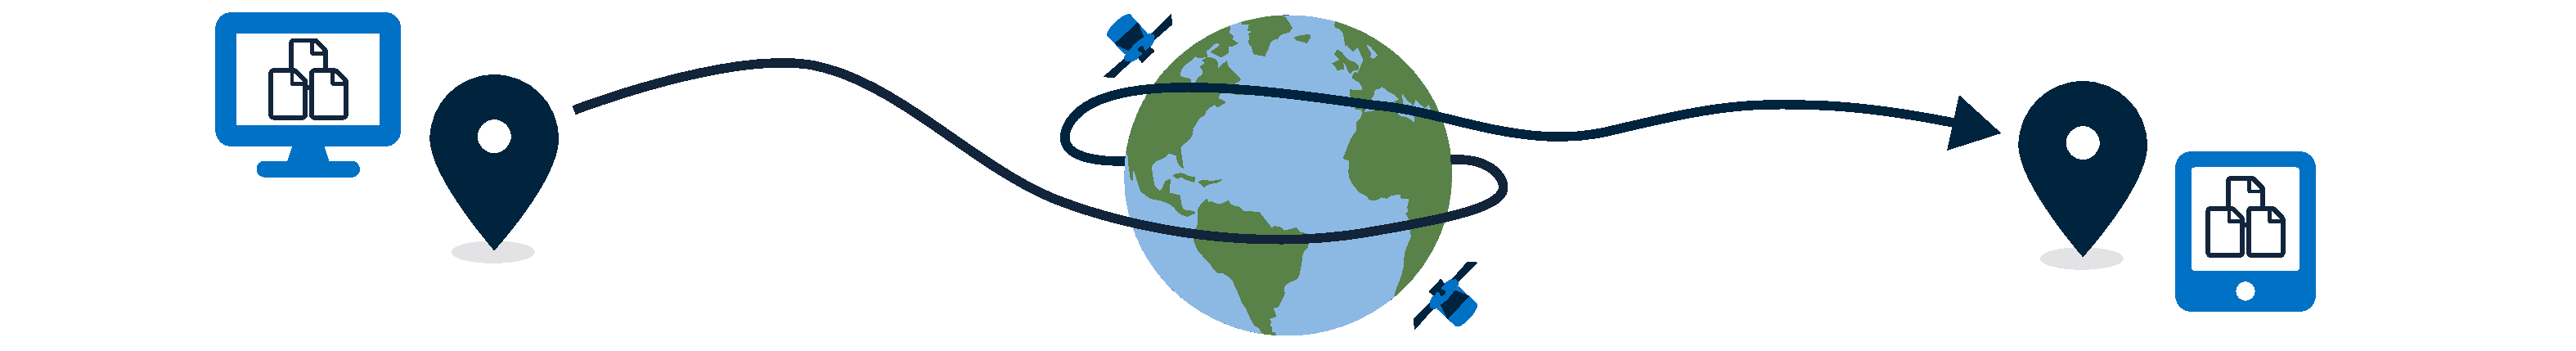
\includegraphics{figures/ch1-earth.pdf}}
    \label{fig:stopsign}
    \vspace{-4mm}
\end{figure}

Sifting through such large volumes of information online to find the elusive and proverbial \emph{needle in the haystack} has been an area of active research and development over a number of decades. Since the early 1990's, the~\gls{acr:www} has emerged as the dominant means of publishing information online over the Internet, replacing obsolete technologies such as the \emph{Gopher} protocol.\footnote{Gopher was designed primarily with a menu-driven interface in mind (i.e. selecting options from a series of choices). The Gopher ecosystem provided the foundations for the~\gls{acr:http} protocol, which the~\gls{acr:www} today utilises.}. As the amount of information available on the~\gls{acr:www} grew\footnote{According to \url{http://www.internetlivestats.com/total-number-of-websites/}, September 2014 saw the point at which 1 billion unique websites were present on the~\gls{acr:www}.\urlaccessed{2018-05-21}}, so too did the paradigms that were employed by those wishing to seek information on it.

Over the course of the \emph{noughties}, the approach demonstrated by \emph{information seekers} for finding information online changed from the concept of \emph{surfing} a particular domain by following a series of set~\glspl{glos:hyperlink} within documents, to explicitly \blueboxbold{searching} the ever increasing universe of documents available at their disposal (refer to Figure~\ref{fig:ch1-surfing}).\footnote{Indeed,~\cite{mcbryan1994taming_tools} considered a search engine as a means of \emph{taming} the considerable number of documents online.} This is not to say that surfing no longer occurs; procrastinators (the author included...) might find solace by surfing the myriad of content available on \emph{Reddit,} billed as the \emph{``front page of the Internet''}\footnote{\url{https://www.reddit.com}\urlaccessed{2018-05-21}}. However, for a task where an individual has a specific \emph{information need,} searching become by far the most dominant paradigm for seeking required information. As such, the development of effective \emph{search engines} has been of paramount importance, with the development of search engines seen as the \emph{raison d'\^{e}tre} of the study of~\gls{acr:ir}.

\begin{figure}[t!]
    \centering
    \resizebox{1\hsize}{!}{
    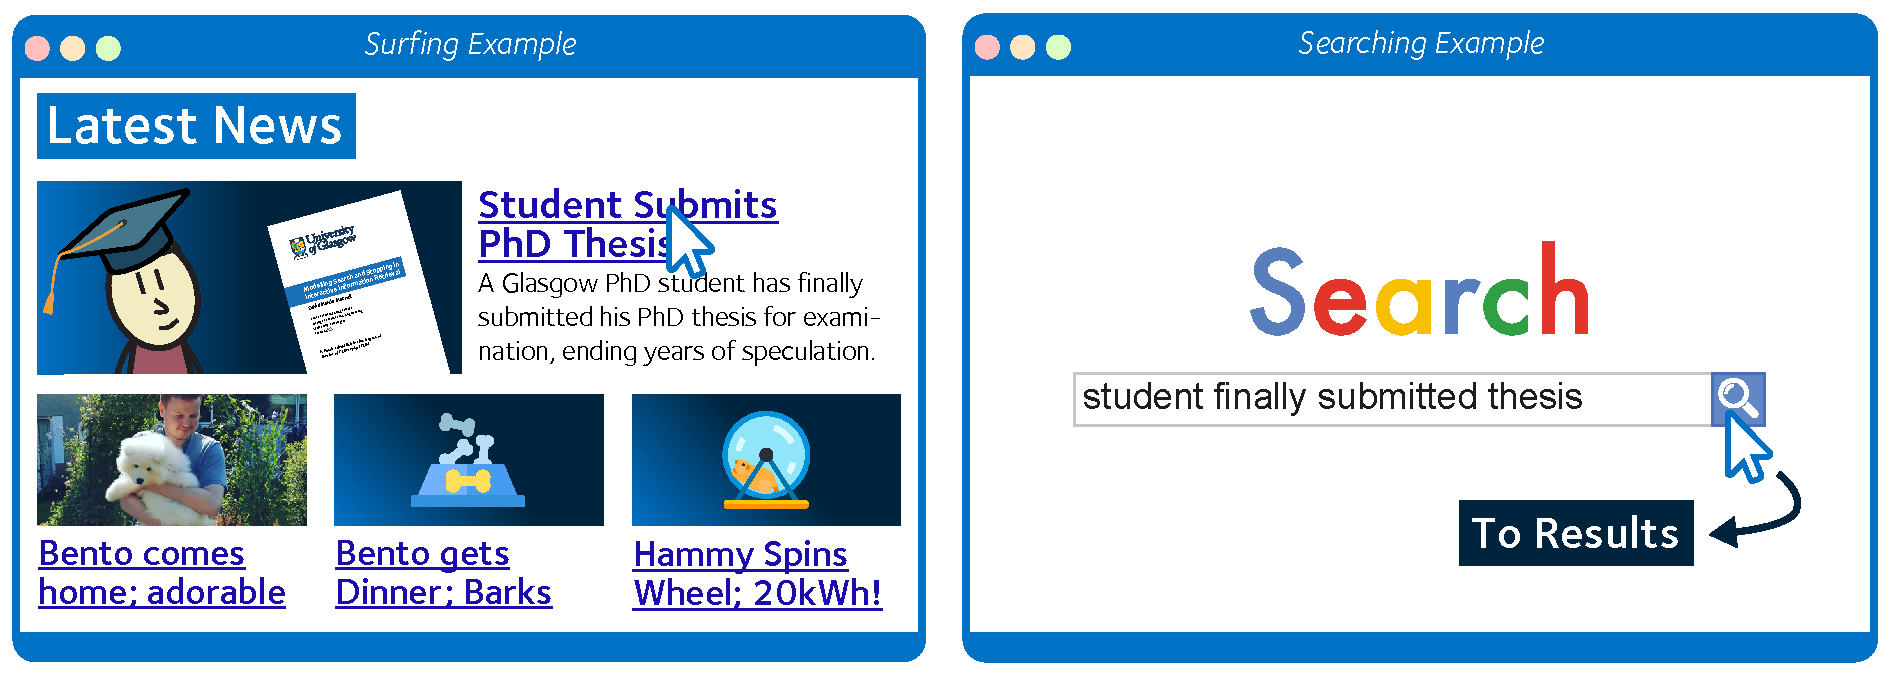
\includegraphics{figures/ch1-surfing.pdf}}
    \caption[Surfing vs. Searching]{The paradigms of surfing and searching. On the left, a seeker will navigate through a series of documents via~\glspl{glos:hyperlink} (perhaps without a specific \emph{information need} in mind), while a searcher (right) will issue a \emph{query} articulating their information need, relying on an underlying \emph{search engine} to \emph{retrieve} documents that it thinks will assist the seeker.}
    \label{fig:ch1-surfing}
\end{figure}

\begin{quote}
    \emph{``...but perhaps the key technology that took the web from a useful supplement of current information practice to become the default communication medium is search.''}
    \attrib{\cite{wilson2010keyword_search}}
\end{quote}

Contemporary search engines such as \emph{Google} and \emph{Bing} are considered to offer an effective means of finding the proverbial needle in the haystack~\citep{wilson2010keyword_search}, where near perfect accuracy is regularly attained for popular \emph{queries}~\citep{vaughan2004new_measurements}. These search engines, along with the many others in existence today under a variety of different contexts\footnote{Google and Bing may be the most popular search engines for \emph{general web queries,} but other contexts can include patent search, enterprise search and multimedia search, as examples.}, are the product of the collective work undertaken in the field of~\gls{acr:ir} -- from early research in the 1970's~\citep{cleverdon1962cranfield_experiments,rijsbergen1979ir}; to the development of various \emph{retrieval models}~\citep{robertson2009probabilistic_models}; to the setting up of \emph{evaluation forums}~\citep{harman1993trec1}; to the development of the \emph{large-scale search engines} (or \emph{retrieval systems}) that are commonplace today~\citep{baezayates1999modern_ir, wang2010language_models}.

The work that the field of~\gls{acr:ir} collectively undertakes is all done in the interests of making it easier for potential users of search engines to satisfy their underlying \emph{information need}. Armed with a preexisting knowledge of the world, an individual will develop an information need from a perceived problem -- either from a knowledge gap, an internal consistency, or a conflict of evidence. This state has been referred to as the \emph{anomalous state of knowledge}~\citep{belkin1980ask}. A searcher then formulates a \emph{query} -- an expression of what they are looking for~\citep{borlund2003iir_model}, typically consisting of a number of different terms -- before being presented with a potentially relevant set of documents. From this set of documents, an individual can then begin the process of examining them for relevance. A number of complex interactions take place between an individual seeking information and the search engine that is being utilised~\citep{ingwersen2005theturn}. This process, where the searcher engages in \emph{dialogue} with the search system, is considered the study of~\glsfirst{acr:iir}~\citep{borlund2003iir_model}. As such, work has been undertaken that attempts to help us better understand these complex interactions, and potentially assist in making the search process a more seamless experience.

\section{Motivation and Context}\label{sec:intro:motivation}
Central to much of the work undertaken in the field of~\gls{acr:ir} over the past 50 years is the so-called \emph{Cranfield paradigm}, a term denoting a standardised approach for the \emph{evaluation} of~\gls{acr:ir} systems. The Cranfield paradigm descends directly from \emph{Cranfield II}~\citep{aslib1966factors}, a set of experiments designed to evaluate the efficiency of \emph{indexing systems}\footnote{The process of indexing, as discussed later in Section~\ref{sec:ir_background:basics:indexing}, involves turning a number of source documents into a form of data structure that can be traversed, or \emph{searched,} in a quick and efficient manner.}. At the time, searching for information on computer systems was achieved through the issuance of queries to a \emph{boolean retrieval system} (refer to Section~\ref{sec:ir_background:basics:models:boolean}), with terms matched against a small set of manually indexed documents~\citep{harman2010cranfield}. Results were compared against a set of \emph{a priori} \emph{relevance judgements} for each of the documents, as judged by humans, allowing one to then ascertain the performance of a given retrieval system.
%We discuss this high-level approach in Section~\ref{sec:ir_background:basics:cranfield}.

While the basic principles of the Cranfield paradigm have remained in place since it was established in the 1960's, components of the approach have evolved over the years to cater for the ever increasing complexity of the tasks at hand~\citep{harman2010cranfield}. Indeed, the approach is still widely used in evaluation forums, such as the~\gls{acr:nist} sponsored~\gls{acr:trec} -- the first of which was held in 1993~\citep{harman1993trec1}. Indeed, many of the relevance judgements and \emph{topics} (i.e. information needs) provided as part of \emph{\gls{acr:trec} Tracks} over a number of years are used as ground truths throughout the work discussed in this thesis.

This approach however can be argued to remain simplistic in terms of consideration of the complex user interactions that take place during the search process~\citep{borlund2000evaluation_iir,ingwersen2005theturn}. In other words, the Cranfield paradigm broadly fails to consider the complexities of the~\gls{acr:iir} process, where, for example, searchers can issue multiple queries during the course of a search session, and adapt their interactions based upon the perceived quality of the presented ranked list of results for each associated query~\citep{moffat2013users_versus_models}. Selecting good terms to use within a query is difficult yet important~\citep{efthimiadis2000query_expansion}; as such, the initial query posed in a search session often acts as an entry to the search system, followed by phases of browsing and query reformulations~\citep{marchionini1993information_seeking}.

Searchers also will typically abide by the principle of least effort, whereby they strive to minimise the probable average rate of work expenditure over time~\citep{zipf1949behaviour}. Cranfield makes a series of assumptions, namely that that a user will: \emph{(i)} issue a single query; \emph{(ii)} examine documents to a great depth (typically $1,000$ documents); and \emph{(iii)} consider all documents to be relevant. This is largely unrealistic, and numerous researchers have proposed alternatives to the Cranfield paradigm --~\cite{borlund2003iir_model}, for example.

Considering alternatives to the Cranfield paradigm,~\cite{keskustalo2008user_simulation} categorised~\gls{acr:iir} research into four different approaches that allow for the consideration of the complex interactions that take place between a human and the search engine being used. The four approaches, as illustrated in Figure~\ref{fig:ch1-options}, can themselves be divided into two categories. The first category considers approaches that utilise \blueboxbold{real-world searchers}, namely:

\begin{itemize}
    \item[]{\blueboxbold{1} the \blueboxbold{observation of real-world searchers} in real world scenarios (e.g. general web search), through the use of \emph{interaction logs;} and}
    \item[]{\blueboxbold{2} the observation of \blueboxbold{real-world searchers undertaking simulated work tasks} in a lab-based environment (i.e. a \emph{user study}).}
\end{itemize}

The final two options \emph{do not explicitly} consider real-world searchers, but rather aim to mimic their behaviours. These approaches are:

\begin{itemize}
    \item[]{\blueboxbold{3} performing \blueboxbold{simulations of interaction} in a lab-based environment, \emph{sans} real-world searchers; and of course}
    \item[]{\blueboxbold{4} the undertaking of \blueboxbold{traditional, Cranfield style lab-based experimentation}.}
\end{itemize}

\begin{figure}[t!]
    \centering
    \resizebox{1\hsize}{!}{
    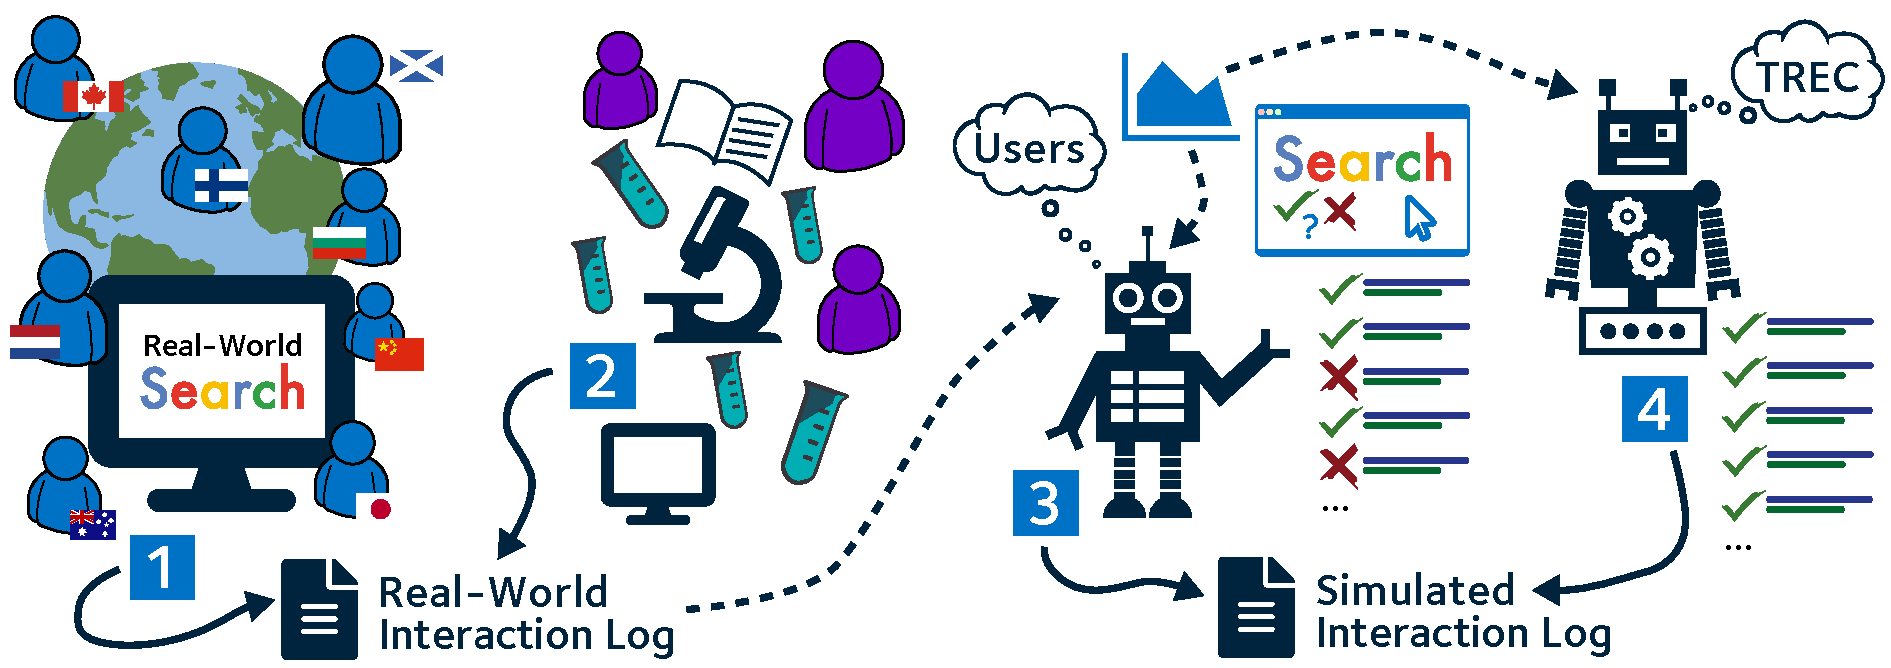
\includegraphics{figures/ch1-options.pdf}}
    \caption[Approaches to~\gls{acr:iir} research]{The four approaches for~\gls{acr:iir} research, as outlined by~\cite{keskustalo2008user_simulation}. Detailed in Section~\ref{sec:intro:motivation}, approaches \blueboxbold{1} \emph{(real-world)} and \blueboxbold{2} \emph{(user studies)} consider log data from real-world searchers, with options \blueboxbold{3} \emph{(simulations of interaction)} and \blueboxbold{4} \emph{(traditional experimentation)} considering log data as generated from \emph{simulations.} Note the \emph{grounding} (dashed line) of log data from either approach \blueboxbold{1} or \blueboxbold{2} to complement approach \blueboxbold{3} (refer to Section~\ref{sec:intro:simulation}).\vspace*{10mm}}
    \label{fig:ch1-options}
\end{figure}

Obtaining interaction data from studies utilising real-world users undertaking search tasks (categories \blueboxbold{1} and \blueboxbold{2}) will of course always be the preferred option. There can never be a better substitute than examining the real thing. However, there are pitfalls with both approaches that must be considered, primarily in terms of \emph{availability} and \emph{cost}. Obtaining data for studies conducted in category \blueboxbold{1} is difficult if the researchers do not work for an organisation offering a large-scale search engine, such as \emph{Google} or \emph{Microsoft.} Working within an academic setting for example may greatly restrict what data can be obtained. Indeed, working with real-world interaction data also leads to major ethical and privacy concerns~\citep{korolova2009aol_query_log_privacy}. The release of the \emph{AOL Query Log} (and subsequent fallout) in August 2006 is testament to that, although this has not stopped researchers from utilising the data in their work (refer to~\cite{brenes2009aol_query_log} for such an example).

This will leave many researchers with category \blueboxbold{2} -- especially those in a non-industrial setting. While this approach also leads to the capturing of real-world interaction data, pitfalls of this approach primarily are the significant costs involved in such an approach -- both financially and in terms of time. Considerations must also be placed into study design to mitigate potential biases. In recent years however, the concept of \emph{crowdsourcing} may alleviate some of these concerns, and open up a potential study to a larger potential audience. A recent study has shown that using crowdsourcing to capture interaction data is no worse than a carefully controlled lab-based user study~\citep{zuccon2013crowdsourcing_comparisons}, although quality control measures must be taken.

While categories \blueboxbold{1} and \blueboxbold{2} provide real-world interaction data, options \blueboxbold{3} and \blueboxbold{4} do not. Such approaches however, if executed correctly, can potentially lead to insights that would not otherwise be possible when involving real-world users. As an example, covering an extensive set of test cases with real-world searchers may simply not be possible~\citep{keskustalo2008user_simulation} -- perhaps due to financial constraints, or a lack of suitable subjects. Category \blueboxbold{4} can be considered as a means of conducting \emph{traditional, TREC-style}~\gls{acr:ir} lab experimentation that is, as previously mentioned, largely na\"{i}ve of the user's complex interactions. This leaves category \blueboxbold{3} as a means of conducting and evaluating user-sided experimentation without the explicit need for real-world users to be present. \blueboxbold{Simulation} is used as a means to conducting such experiments.

\subsection{Considering Simulation}\label{sec:intro:simulation}
Simulation is defined as the \emph{imitation of the operation of a real-world process or system over time}~\citep{banks1996discrete}. Such an approach allows one to gain insight into the functioning of some real-world phenomenon. Simulation has been used in a wide range of areas, including, for example, examining physical processes~\citep{haessig1991physics_modelling}, psychology~\citep{hastie1988human_memory_simulation}, road traffic~\citep{mahmud2016traffic_modelling_electric} and training for various activities, such as piloting an aeroplane~\citep{sparko2010flight_simulators}. Central to contemporary uses of simulation is the idea of \emph{computerised simulation}~\citep{heermann1990computer_simulation}. Thanks to ever increasing computational power in~\glspl{acr:cpu} and~\glspl{acr:gpu} available for such tasks, such as the simulation of racing cars for the purposes of driver development, as shown in Figure~\ref{fig:ch1-mclaren}. With computer simulation, a real-world object can be imitated with varying degrees of realism. Alternatively, individual components that comprise a larger system can be examined and simulated in isolation, allowing researchers to obtain a more detailed understanding of how individual components react to changes in their environment. As such, simulation can provide a rapid means of exploring aspects of a real-world phenomenon, all at a low cost -- all the while permitting repeatable, and therefore reproducible, results~\citep{maxwell2016agents}.

\begin{figure}[t!]
    \centering
    \resizebox{1\hsize}{!}{
    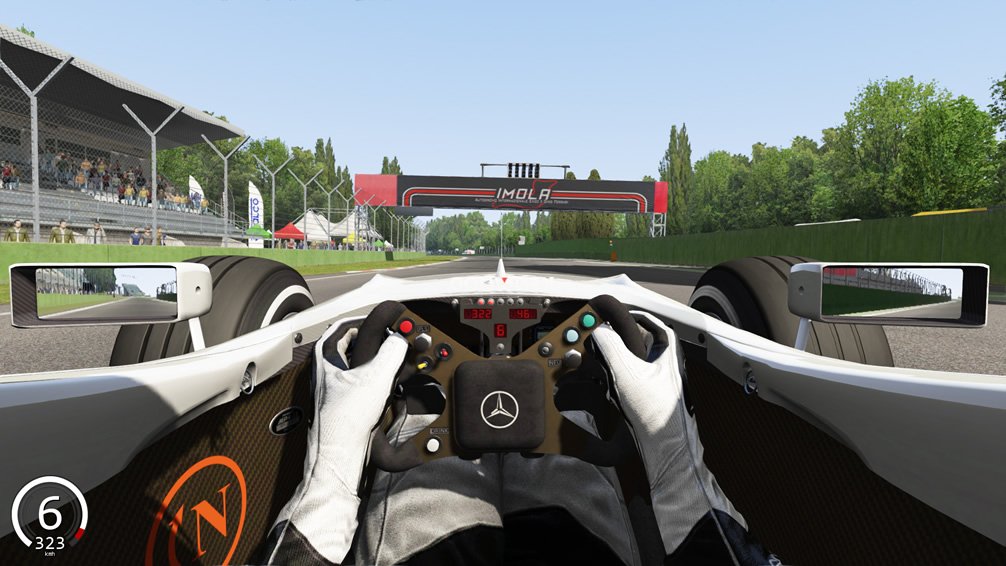
\includegraphics{figures/ch1-mclaren.jpg}}
    \caption[Racing Simulator Example]{An example of a \emph{video game simulation}, \emph{Assetto Corsa}. In this illustration is a model of the \emph{McLaren-Mercedes MP4/13} race car (complete with terrible gear ratios), driving around the \emph{Autodromo Enzo e Dino Ferrari} circuit in northeastern Italy. In the past ten years, increases in~\gls{acr:cpu} and~\gls{acr:gpu} performance has enabled the development of increasingly complex (and \emph{more realistic}) video game simulations, which, for example, are now used in the training of racing drivers.}
    \label{fig:ch1-mclaren}
\end{figure}

One of the key components of any simulation -- regardless of whether it is executed on a computer or not -- is that of an underlying \emph{model} of the real-world phenomenon being simulated~\citep{tocher1963art_of_simulation}. This model defines the various stages, rules and other descriptive components of the phenomenon that simulations must consider. These rules are often high level, and as such, a number of \emph{assumptions} are made~\citep{tocher1963art_of_simulation}. For example, the~\gls{acr:trec} model of search (as detailed in Section~\ref{sec:stopping_background:models}) assumes that a single query is issued by a searcher within a search session, and searchers examine to great depths per query. These assumptions should be made in the face of supporting evidence; evidence in~\gls{acr:iir} studies strongly suggests that searchers do not follow this rigid approach, but rather adapt their behaviour based upon cues that are presented to them.

Why though, use simulation when other alternatives to modelling the search process are available? Alternatives include some form of closed-form system, such as a series of linear equations to describe the complex interactions that take place. However, according to~\cite{fishwick1995simulation}, this approach is not flexible enough, and a number of reasons are linked as to why simulation is essential in complex, dynamic systems:

\begin{itemize}
    \item{the model is very complex, with many variables and interacting components;}
    \item{the underlying variables and relationships are non-linear;}
    \item{the underlying models contains random variates; and}
    \item{the model output is to be visual, as in a three-dimensional computer animation.}
\end{itemize}

In the context of~\gls{acr:iir}, the first three reasons can be considered as acceptable reasons for why simulation is an advantageous methodology to pursue. For example, many state-of-the-art~\gls{acr:iir} models consider a stochastic component when determining the relevancy of a document to a particular information need (or~\gls{acr:trec} topic).

Simulation provides a means of using a uniform model execution technique that can be used to solve a large variety of systems, without resorting to a \emph{``bag of tricks'',} where one must choose special purpose and sometimes arcane solutions to avoid simulation~\citep{fishwick1995simulation}. Simulation provides the freedom and flexibility to permit the implementation of a model that better represents the real-world phenomenon that is being considered. In contrast, with a more closed-form approach, the underlying model that is created is often twisted and altered to suite the closed-form approach, rather than to actually represent the real-world system. This leads to a larger gap between the model and reality, and as such leads to a greater number of assumptions within the model than what would otherwise be required. In other words, the technique used to develop the model constrains just how realistic is can be. Simulation provides the freedom and flexibility to reduce assumptions that may otherwise be included.

As a means of testing better and more flexible models of search, simulation has been extensively used within~\gls{acr:ir}. While we provide an overview of simulation of~\gls{acr:ir} in Section~\ref{sec:ir_background:user:simulation}, one such area that has been studied is \emph{simulated interaction,} where one attempts to mimic the behaviours that a searcher exerts when interacting with a search engine -- and is exactly what we consider in this thesis. While this encapsulates category \blueboxbold{3} of the four categories outlined by~\cite{keskustalo2008user_simulation}, we also argue that in order to run simulations of interaction \emph{`correctly',} they must be \emph{grounded} using real-world observations, which in turn means that the assumptions can be considered to be credible abstractions of the real-world phenomenon. As such, this necessitates access to data obtained through either categories \blueboxbold{1} or \blueboxbold{2} -- or, in other words, data from \emph{real-world searchers.} Without access to a large-scale search engine for this research, this leaves category \blueboxbold{2} as a means for acquiring such data, and provides an explanation between the linking of the real-world interaction log, and simulated users (via the dashed line) in Figure~\ref{fig:ch1-options} on page~\pageref{fig:ch1-options}.

\noindent
\blueboxbold{In a Nutshell – Simulation and this Thesis}
Given all of the above, this thesis proposes a more advanced, realistic model of the search process. In line with the suggestions outlined in the work by~\cite{keskustalo2008user_simulation}, simulations of interaction are trialled (category \blueboxbold{3}), with the underlying components of the model \emph{grounded} using interaction data extracted from two different user studies, also conducted as part of this thesis. One particularly important phenomenon that has been largely overlooked in the~\gls{acr:iir} literature is that of a searcher's \blueboxbold{stopping behaviour} (e.g. \emph{given this list of ranked results, how far down the list should I go before I stop?}). In the next section, we provide a brief introduction on why stopping behaviour is important, before considering this thesis' research statement.

\subsection{Considering Stopping Behaviours}\label{sec:intro:stopping}
\begin{wrapfigure}[7]{r}{0.45\textwidth}
    \begin{center}
    \vspace*{-13mm}
    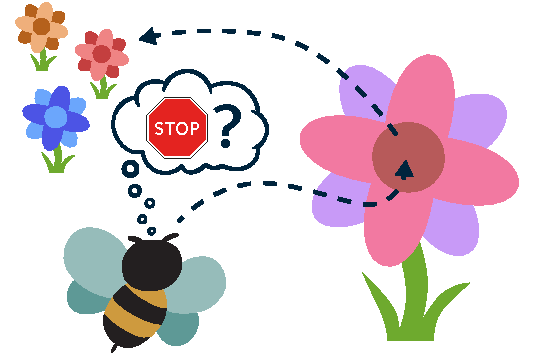
\includegraphics[width=1\textwidth]{figures/ch1-bee.pdf}
    \end{center}
    \vspace*{-4mm}
    \label{fig:bee}
\end{wrapfigure}

With any activity that a creature makes, there has to come a time when it makes a decision to \emph{stop} what it is doing. A honeybee, when collecting pollen on a flowerhead, will eventually stop collecting and fly away to another flower. An exhausted PhD student, when writing his or her thesis, will eventually stop writing for the night once he or she has become too tired -- something the author knows only all too well. Similarly, when applied to the context of search, an individual will also make a decision to eventually stop examining content. These examples demonstrate that knowing when to stop is a fundamental aspect of animal -- and by definition, human -- thinking and behaviour.

But given this, what actually makes us decide when to stop doing something? Obviously, different \emph{external factors} can influence this decision, such as finding no more pollen on a flowerhead, or time pressure that is exerted upon us. Moreover,~\citep{nickles1995judgment} argues that \emph{knowing when to stop} is largely determined by a series of \emph{internally defined, stopping criteria} that the decision maker employs. This makes stopping a phenomenon that is incredibly difficult to model effectively. We discuss this in more detail in Section~\ref{chap:stopping_background:why}.

Given the fact that internal factors are a major drive to determining when to stop, studies have largely been unable to quantify \emph{why} searchers stop, other than what they find gives them the feeling that it is \emph{``good enough''}~\citep{zach2005enough_is_enough}. Researchers have however attempted to create a series of \emph{reasoning} and \emph{judgement} based \blueboxbold{stopping heuristics} that attempt to formally define when a searcher should stop. It is these stopping heuristics that we will primarily consider in this thesis. In conjunction with an updated user model of search, these heuristics can then be integrated into the model, allowing us to determine whether they offer better or worse approximations of actual searcher stopping behaviours.

Examining stopping behaviour during search is important because it considers the judgements of a searcher as part of their interactions. For example, it would be prudent of a searcher examining a list of results that are mostly considered to be non-relevant to a given information need to stop early, and thus save time and effort. In other words, a good stopping heuristic allows a searcher to become \emph{more efficient.} This can be achieved in a number of different places -- or \blueboxbold{stopping decision points} -- during search, such as the depth to which a searcher will examine a list of results.

\section{Overarching Research Questions}\label{sec:intro:rqs}
From the introductory explanations of the problem space above, we can now formulate the four main overarching, high level research questions -- denoted as \blueboxbold{HL-RQ} -- that the work in this thesis addresses. Our first research question considers the concept of user modelling, and how, with an emphasis of examining stopping decision points, we can improve the current model to better reflect actual searcher behaviours.

\begin{itemize}
    \item[]{\blueboxbold{HL-RQ1} How can we improve the current state-of-the-art searcher model to incorporate different points where individuals subscribing to such a model can stop?}
\end{itemize}

As previously stated, being able to improve the current state-of-the-art from a stopping perspective should allow those subscribing to such a model to become more efficient at how they search. Closely related to this advancement in user modelling is the consideration of the various stopping heuristics, as briefly outlined in Section~\ref{sec:intro:stopping}.

\begin{itemize}
    \item[]{\blueboxbold{HL-RQ2} Given the stopping heuristics defined in the literature, how can we encode these heuristics into a series of operationalised, programmable \blueboxbold{stopping strategies} that can be subsequently evaluated?}
\end{itemize}

The heuristics that we detail later in Section~\ref{sec:stopping_background:heuristics} are high level in nature, and no not provide an explanation as to how they can be \emph{operationalised} within a wider system. The challenge that must be addressed in order to answer this question will be how we can operationalise these heuristics within a wider, common framework.

Our final two overarching research questions can be considered similar in nature, and are numbered as such. With a more realistic model of the search process defined by addressing \blueboxbold{HL-RQ1} and a series of stopping strategies defined by addressing \blueboxbold{HL-RQ2}, how well do the combinations of an improved model and different stopping strategies perform?

\begin{itemize}
    \item[]{\blueboxbold{HL-RQ3a} Given these operationalised stopping strategies, how well do simulated searchers using these strategies perform?}
    \item[]{\blueboxbold{HL-RQ3b} How closely do the operationalised stopping strategies compare to the stopping behaviours of real-world searchers?}
\end{itemize}

With the flexibility provided by the approach, simulation is an ideal mechanism for achieving a means to address these two research questions. These questions are of course very broad in nature -- as should be expected for overarching questions -- and it is simply not possible to evaluate them in every conceivable search context. As we discuss in the following section, we will examine these questions in several different contexts which are likely to impact upon the stopping behaviours of searchers.

\section{Thesis Contributions}\label{sec:intro:contribs}
From our four overarching research questions defined above, we identify four major contributions offered by the work presented in this thesis. Listed and detailed below, we consider primary contributions from conceptual, theoretical and empirical standpoints. We also consider the general methodology that we utilise throughout the work in this thesis.

\noindent
\blueboxbold{Conceptual Model}
Our first contribution is that of a searcher model. Taking the current state-of-the-art, we propose an updated, high-level model of the search process. We call this model the \blueboxbold{\gls{acr:csm}}, and this provides us with a solution for addressing \blueboxbold{HL-RQ1}. Outlined in Section~\ref{sec:csm:csm}, the conceptual~\gls{acr:csm} outlines a series of different activities and decision points that searchers undertake throughout the search process, and establishes a flow of interaction based upon established models. Within the~\gls{acr:csm} are a number of innovations, central to the work in this being a new stopping decision point. Combined together, these improvements allow us to ascertain a better understanding of the search process, and the complex interactions between a searcher and search system that take place. Being a conceptual model, we can take the~\gls{acr:csm} and instantiate it in a number of different ways. For example, the stopping decision points (i.e. \emph{should I continue examining this set of results?}) must be instantiated -- and for this, our second contribution provides a solution to this problem.

\noindent
\blueboxbold{Theoretical Examination}
As briefly outlined in Section~\ref{sec:intro:stopping}, there are a range of different stopping heuristics that have been defined in the literature -- some directly applicable to search, some defined in other branches of science (such as ecology, for example). The second major contribution of this thesis is the development of a series of operationalised, programmable stopping strategies that can be subsequently implemented as a stopping decision point of the~\gls{acr:csm}, defined above. These are delivered within a common framework. These operationalised stopping strategies provide a solution to our second overarching research question, \blueboxbold{HL-RQ2}.

\noindent
\blueboxbold{Empirical Studies}
As discussed in Section~\ref{sec:intro:rqs}, the~\gls{acr:csm} and the various stopping strategies that we operationalise need to be evaluated, such that we can then subsequently address \blueboxbold{HL-RQ3a} and \blueboxbold{HL-RQ3b}. To do this, the third major contribution of this thesis is empirical. We conduct two user studies, choosing to examine different factors which are likely to affect stopping behaviours. These factors are:

\begin{itemize}
    \item{varying snippet length (and subsequently snippet quality);}
    \item{varying task goals -- from time-limited to \emph{find $x$ relevant items}; and}
    \item{varying task type, considering \emph{ad-hoc topic retrieval} and \emph{diversifying results.}}
\end{itemize}

These studies are part of the \blueboxbold{general methodology} that we utilise. After the user studies have been completed and stopping behaviours investigated empirically, we then use the data from these studies to ground a series of simulations, as discussed in Section~\ref{sec:intro:simulation}. This improves the credibility of the simulations, which are then examined, and allow us to: address which stopping strategies (under a certain context); offer \blueboxbold{HL-RQ3a} the best overall performance; and \blueboxbold{HL-RQ3b} closest approximations to actual searcher behaviours. Simulations are conducted entirely using a custom built simulation framework, \blueboxbold{SimIIR}.

\section{Thesis Statement}
Given the above, the statement of this thesis is that by considering additional stopping decision points within a model of the interactions between a searcher and a search system, one can run simulations of interaction that offer a greater degree of realism of searcher behaviour. Thus, this leads to us acquiring a more comprehensive understanding of the complex interactions that take place.

%Thus, one should be able to deduce an optimal \emph{stopping strategy} yielding high performance, and a better approximation of the actual behaviours exhibited by real-world searchers than currently employed models.

In particular, incorporating such stopping decision points within a model of the search process will allow a simulated user abiding by it a greater degree of flexibility in the search strategy that they employ. For example, a searcher will be able to abandon a set of results that is judged to be of low relevance to a given information need. This will allow abandonment comparatively earlier than a set of results that are perceived to be of higher quality. In addition, these stopping decision points can be instantiated by operationalising a series of different stopping heuristics that are \emph{believed}~\citep{maxwell2015stopping_strategies} to encapsulate the stopping behaviours exhibited by real-world searchers. By taking this knowledge forward, we can then ground these simulations of interaction over a variety of different search contexts with differing goals, examining how the stopping behaviours of searchers varies under each context. Through simulation, we can then deduce what particular heuristic(s) offer the best performance and best approximations to actual searcher behaviours.

\section{Origins of the Material}
Material presented in this thesis has appeared in several conference papers throughout the duration of the author's PhD programme, from October 2013 to June 2018. All are listed in the front matter of this thesis in chronological order. In this section, we provide narrative, explaining how the developments in the listed publications led to the contributions of this thesis, listed above. Work can be considered over three main strands:

\begin{itemize}
    \item{the development of the conceptual and theoretical contributions to this work;}
    \item{the development of the SimIIR framework; and}
    \item{a series of empirical studies.}
\end{itemize}

\noindent
\blueboxbold{Conceptual and Theoretical}
Work on the~\gls{acr:csm} has been undertaken over a number of years. A number of iterations of the~\gls{acr:csm} were presented in various publications. However, in order to simplify the work reported in this thesis, we consider only the latest iteration. The first version of the~\gls{acr:csm}, essentially analogous to the prior models of search outlined in Section~\ref{sec:stopping_background:models:conceptual:simple}, were outlined and used in simulated analyses, as reported in two publications.

\begin{itemize}
    \item{\bibentry{maxwell2015initial_stopping}}
    \item{\bibentry{maxwell2015stopping_strategies}}
\end{itemize}

These publications are notable for also including a number of operationalised stopping strategies, providing the foundations for the second major contribution of this thesis. The stopping strategies defined in these publications were used in subsequent publications. Further developments to the~\gls{acr:csm} were found in a subsequent publication which experimented with the notion of \emph{intelligent search agents}.

\begin{itemize}
    \item{\bibentry{maxwell2016agents}}
\end{itemize}

The final development of the~\gls{acr:csm} led to the inclusion of a third stopping decision point, complete with a large-scale simulated analysis. This led to the finding that the inclusion of the new decision point within the~\gls{acr:csm} led to improvements in overall search performance, and approximations of actual searcher behaviours.

\begin{itemize}
    \item{\bibentry{maxwell2018serp}}
\end{itemize}

\noindent
\blueboxbold{SimIIR Framework}
One of the major pieces of scientific apparatus utilised throughout all of the aforementioned studies is the SimIIR framework, touched upon in Section~\ref{sec:intro:contribs}. While we do not explicitly discuss the framework in great depth in this thesis, but rather focus on how we implemented the different components, conducting the simulated analyses would not have been possible without it. A publication demonstrating the framework and the various components that could be instantiated was published.

\begin{itemize}
    \item{\bibentry{maxwell2016simiir}}
\end{itemize}

\noindent
\blueboxbold{Empirical Studies}
The general methodology that we employ for the third major contribution of this thesis has been introduced and refined in the publications listed previously. In addition to this, a basic description of the methodology is provided in a Doctoral Consortium paper that the author presented at the first \emph{ACM Conference on Human Information Interaction and Retrieval (CHIIR)} in Chapel Hill, NC, USA.

\begin{itemize}
    \item{\bibentry{maxwell2016dc}}
\end{itemize}

The results of two studies were also published, and are of direct relevance to the work detailed later in this thesis.

\begin{itemize}
    \item{\bibentry{maxwell2014temporal_delays}}
    \item{\bibentry{maxwell2017snippets}}
\end{itemize}

These studies provide the grounding for simulated analyses that we also consider later in this thesis. The data extracted from these user studies provides credibility to our simulations, through the extraction of aspects such as interaction costs and probabilities.

\section{Remaining Thesis Outline}
Now that our motivation, research questions and thesis contributions have been outlined, this section provides a brief summary of the remaining chapters of the thesis. Split into four parts, the chapters are summarised below.

\noindent
\darkblueboxbold{Part I}
The remainder of Part I concerns prior work that has been undertaken in the fields of~\gls{acr:ir} and~\gls{acr:iir}. Two chapters discuss the basics of~\gls{acr:ir} and~\gls{acr:iir}, before we begin to examine prior work that considers search and stopping.

\begin{itemize}
    \item[]{\blueboxbold{Chapter 2}} Beginning on page~\pageref{chap:ir_background}, this chapter provides an overview of the key concepts of the fields of~\gls{acr:ir} and~\gls{acr:iir}. In particular, we focus on basic~\gls{acr:ir} concepts such as the indexing and retrieval processes (including retrieval models), before moving towards a more user-centric examination of various evaluation measures that are commonly deployed in~\gls{acr:iir} research.
    
    \item[]{\blueboxbold{Chapter 3}} We then consider work that has been undertaken in relation to stopping behaviours. In this chapter, we focus on the development of various stopping heuristics, examine previous studies that have examined searcher stopping behaviours, examine key theoretical models of search that provide explanations for when individuals stop, and finally discuss prior models of search -- focusing particularly on the components that consider stopping behaviours. 
\end{itemize}

\noindent
\darkblueboxbold{Part II} Beginning on page~\pageref{part:stopping}, Part II begins to consider the conceptual and theoretical contributions of this thesis, including a discussion of the~\gls{acr:csm}. We also in this part of the thesis provide an outline of the general methodology that is extensively utilised in Part III.

\begin{itemize}
    \item[]{\blueboxbold{Chapter 4} This chapter introduces the~\gls{acr:csm}, discussing the advancements the conceptual model provides over the current state-of-the-art. We discuss the key stopping decision points provided by the~\gls{acr:csm} that are central to this thesis, before discussing the assumptions of the model.}
    
    \item[]{\blueboxbold{Chapter 5} In this chapter, we introduce and discuss the various stopping strategies that we operationalise as part of the contributions of this thesis. Each of the different stopping strategies are discussed in depth, complete with examples of each. The chosen stopping strategies are linked back to their source stopping heuristics, which are detailed in Chapter~\ref{chap:stopping_background}.}
    
    \item[]{\blueboxbold{Chapter 6} The third chapter of this part outlines our general methodology, detailing the high-level structure of the scientific method used in the empirical work discussed in Part III. We also provide in-depth discussion of common approaches that were followed across all subsequent chapters, providing a neat overview of the work that was undertaken.}
\end{itemize}

\noindent
\darkblueboxbold{Part III}
The third part of this thesis considers the empirical contributions that are made. In this part, we discuss the user studies that were undertaken, as well as a number of simulated analyses that allow us to address research questions \blueboxbold{HL-RQ3a} and \blueboxbold{HL-RQ3b}.

\begin{itemize}
    \item[]{\blueboxbold{Chapter 7} This first empirical chapter considers how a searcher's behaviour varies when the length (and subsequently quality) of snippets is varied. We provide a discussion of a user study that examined this phenomenon, before summarising the findings of a simulated analyses that was conducted in order to determine what stopping strategies offered the best performance and approximations under this context.}
    \item[]{\blueboxbold{Chapter 8} A similar approach to the chapter above is followed here, with a variation on the user study discussed and subsequently simulated. In this chapter, we examine how a searcher's stopping behaviour varies when subjected to different constraints and task goals, considering time limits, \emph{find $x$} and diversified and non-diversified tasks.}
    \item[]{\blueboxbold{Chapter 9} This final contributory chapter of the thesis considers the new stopping decision point that is provided by the~\gls{acr:csm}. We empirically test the~\gls{acr:csm}, allowing us to determine whether the inclusion of the new stopping decision point discussed in Chapter~\ref{chap:csm} provides improvements in overall performance and approximations of actual searcher behaviours. Conducted via simulation, we utilise data from user studies discussed in prior chapters to ground these reported simulations.}
\end{itemize}

\noindent
\darkblueboxbold{Part IV} Consists of a single chapter, \blueboxbold{Chapter 10}. This concluding chapter of this thesis provides a summary of the work that was undertaken, and the results that were subsequently found. We then consider the results and discuss what they mean in terms of directions for future work.





% From the introductory explanations of the problem space above, we can now enumerate the three main contributions that this thesis provides to the community.
%
%
% This thesis offers four main contributions to the research community, revolving around the concepts of user modelling and stopping behaviours during search.
%
% \begin{itemize}
%     \item[\blueboxbold{C1}]{We provide a series of contributions on user modelling within the IIR process. Specifically, we focus on the development of accepted user models by incorporating additional \textbf{stopping decision points}, and incorporating the ability for a simulated user to remember what has been examined through the inclusion of some basic \textbf{form of state}.}
%
%     \item[\blueboxbold{C2}]{The second main contribution is the \textbf{SimIIR framework}, developed to allow for the running of \textbf{simulations of interaction}. Within the framework, our proposed user model is encoded, along with the ability to specify and configure various components of the search process. An explanation of the framework is provided in Appendix~\ref{appx:simiir}.}
%
%     \item[\blueboxbold{C3}]{We provide a comprehensive survey on various s\textbf{topping heuristics} that have been proposed over the years in the literature, before providing analysis on how performance and behavioural characteristics vary when considering:}
%
%     \begin{itemize}
%         \item{Snippet-Level stopping and associated strategies;}
%         \item{SERP-Level stopping; and}
%         \item{Session-Level stopping.}
%     \end{itemize}
%
%     \item[\blueboxbold{C4}]{Finally, we provide analysis examining how the \textbf{stopping behaviour of searchers varies under different search contexts}, such as when we vary the overall search goal, or vary presentational aspects of the presented results.}
%
% \end{itemize}

% Moved in May, 2018
%%%

% As previously mentioned, knowing when to stop is a fundamental aspect of human thinking and behaviour. Humans and other animals when interacting with the world will employ some form of \emph{stopping criterion} to decide when they should stop~\citep{nickles1995judgment}. As an example, a shopper who is looking to purchase a new smartphone will stop shopping around once he or she has obtained sufficient information on what new smartphone to purchase. Once their case notes for a patient have been compiled, a medical doctor will then be in a position to diagnose the patient's ailment.
%
% The decision of when to stop is not exclusively due to factors external to the decision maker, but rather from a series of \emph{internal, cognitive factors} of their thinking process~\citep{nickles1995judgment}. An individual who is hungry will stop eating once he or she is no longer hungry, rather than stopping when all of the food presented to him or her has been consumed. Empirical research has over the years demonstrated that individuals, regardless of the task presented to them, will frequently stop prematurely. Indeed, this na\"{i}ve behaviour demonstrates that individuals may be willing to go with what \emph{``sounds right''} to them -- often minimising the cognitive effort that is required at the expense of greater accuracy~\citep{perkins1983difficulties}. However, this lower level of potential accuracy does lead searchers to making a greater number of errors in their decision making~\citep{baron1988heuristics}, with individuals overlooking important elements, and potentially miss out useful information~\citep{fischhoff1977cost_benefit, fischhoff1978fault, shafir1992thinking}, with the individual then failing to consider alternatives~\citep{farquhar1993decision_structuring}.
%
% Based upon prior research into the phenomenon of stopping behaviour, it is clear that this is driven primarily from internal factors. As such, we then consider: \emph{what aspects of the decision maker's thinking processes prompt him or her to stop assessing the information provided?} Knowing when to stop requires that the individual in question makes a \emph{judgement} regarding the sufficiency of the information obtained, and whether or not additional information is required to be obtained~\citep{browne2004stopping_rules}. This judgement is normally characterised by both the completeness and correctness of the information obtained thus far~\citep{smith1991belief}. These claims can be mirrored by qualitative studies on examining stopping behaviour, where researchers have found that searchers stop examining a ranked list of results simply because what they have found previously is \emph{``good enough''}~\citep{zach2005enough_is_enough}, echoing the reasoning that individuals will be happy to stop when what they have found \emph{``sounds right''}~\citep{perkins1983difficulties}.

%%%



% \todo{This is essentially duplicated in Chapter 3.} Knowing when to stop is a fundamental aspect of human thinking, with individuals commonly employing some form of \emph{stopping criterion} to decide when they should stop with their interactions in the world around them~\citep{nickles1995judgment}. As an example, a shopper looking to buy a new smartphone will stop shopping around once he or she has obtained sufficient information on what new device to purchase. A doctor, once their case notes about a patient's condition have been finished, will then diagnose their ailment. In the context of search, stopping may be considered at a variety of different points during the search process. The commonly used example of \emph{search stopping behaviour} is the point at which a searcher should stop examining a list of ranked results, or, in other words, \emph{how far down the ranked list the searcher should go}, for example.
%
% The decision of when to stop is not necessarily due to external factors, but from a series of \emph{internal factors} of the decision maker's thinking process. In the context of informational search, knowing when to stop requires that the individual makes a judgement regarding the sufficiency of the information obtained, and whether or not additional information is required to be obtained~\citep{browne2004stopping_rules}. This is normally characterised by both the completeness and correctness of the information obtained thus far~\citep{smith1991belief}. These claims can be mirrored by qualitative studies on examining stopping behaviour, where researchers have found that searchers stop examining a ranked list of results simply because what they have found previously is \emph{``good enough''}~\citep{wu2014information_scent}.
%
% Considering the above, is there any means by which we can quantify what this feeling of \emph{``good enough''} actually is? Researchers have devised a series of different \emph{stopping heuristics} as a means to try and encapsulate the differing stopping behaviours exhibited by searchers. However, the literature in examining which of these heuristics offers the best approximations to what searchers actually do is somewhat limited. By focusing on stopping behaviour within this thesis, our model provides additional points at which a simulated user can stop interactions with a search engine, and thus save time and effort that might otherwise have been wasted if they continued to examine content.

% End May 2018 move

% \todo{======}
%
%
%
%
% \section{Motivation and Context}
% Central to the~\gls{acr:ir} community is the so-called \emph{Cranfield Paradigm}, which represents a standardised approach for the evaluation of~\gls{acr:ir} systems. The paradigm was designed in the early 1960's, when information access was largely achieved through the issuance of boolean queries against manually indexed documents~\citep{harman2010cranfield}. Initial experiments, known as the \emph{Cranfield Experiments}~\citep{cleverdon1962cranfield_experiments}, focused on a single query and associated relevance judgements.
%
% While explained in more detail in Chapter~\ref{chap:background}, the Cranfield paradigm has remained in use to this day, being the \emph{de facto} approach employed by various~\gls{acr:ir} evaluation forums, such as the \emph{NIST}-sponsored \emph{Text REtrieval Conference (TREC)}. Indeed, many of the \emph{relevance assessments} and \emph{topics} provided as part of \emph{TREC Tracks} over the years are used as ground truths throughout the work discussed in this thesis. While components of the paradigm have evolved over the decades as underlying tasks have become more complex~\citep{harman2010cranfield}, the approach however can be argued to remain simplistic in terms of when considering the complex user interactions that take place during the search process~\citep{ingwersen2005theturn, borlund2000evaluation_iir}. In other words, the Cranfield Paradigm broadly fails to consider the complexities of the~\gls{acr:iir} process, where, for example, searchers adapt their interactions baed upon the perceived quality of the presented rank list of results~\citep{moffat2013users_versus_models}.
%
%
% A searcher approaches an Information Retrieval (IR) system with a need for information derived from an ‘anomalous state of knowledge’ (Belkin et al., 1982). This need is typically transformed into a query statement, submitted to the system and a set of potentially relevant documents is retrieved and presented. The transformation of this need into a search expression, or query, is known as query formulation. Through such transformations and further interaction searchers can conduct Interactive IR (IIR), where they engage in dialogue with the IR system and it dynamically responds to their feedback (Borlund, 2003).
%
%
% ~\citep{borlund2003iir_model}
%
%
%
%
% Central to the Information Retrieval community is the so-called Cranfield Paradigm, having been established since the 1960's. This approach leads to reproducibility of experiments, and sensible approach to providing a means of evaluation for improvements of ranking algorithms, for example. Indeed, this approach is still widely used in IR today. Every year, TREC uses this approach. NTCIR and other TREC-inspired conferences use this approach. The approach provides the community with document assessments, which are difficult to procure, and promotes that reproducibility.
%
% What about the user? In an age where information is expected to be found almost instantaneously, people demand a search engine that works. And indeed, we broadly do have that in \emph{Google} -- as per Max Wilson. But do we really have a solid understanding of the complex interactions that take place between a searcher and a human? The field of IIR tries to address this gap in our knowledge.
%
% a user will typically abide by the principle of least effort -- striving to minimise the probable average rate of work expenditure over time (zipf, 1949)
%
% This need is typically transformed into a query statement, submitted to the system and a set of potentially relevant documents is retrieved and presented. The transformation of this need into a search expression, or query, is known as query formulation. Through such transformations and further interaction searchers can conduct Interactive IR (IIR), where they engage in dialogue with the IR system and it dynamically responds to their feedback (Borlund, 2003).
%
% IIR is a complex process in which people issue a multiple queries in a session (The Turn). One central argument is that the Cranfield Paradigm is essentially na\"{i}ve of the complex interactions that take place. Cranfield can be considered to issue a single query, typically the title of a topic, and examine to a large depth (typically 1000), while assuming that all documents are relevant. We know, as humans, that this is not representative of real-world searchers. We know that searchers adapt their behaviour due to a variety of factors, perhaps most notably due to the perceived quality of the returned list of ranked results. They \emph{adapt}. TREC users do not.
%
% When considering users, a number of different approaches have been considered. Keskustalo
%
% \begin{itemize}
%
%     \item[\blueboxbold{1}]{the analysis of log data collected from real-world scenarios (e.g. from commercial web search engines);}
%     \item[\blueboxbold{2}]{the collection of interaction data from simulated search tasks (e.g. a lab-based user study);}
%     \item[\blueboxbold{3}]{the simulation of interaction, considering the user and the various processes that are undertaken -- sans users -- and}
%     \item[\blueboxbold{4}]{`traditional' lab-based studies, sans users, aka TREC-style experimentation.}
%
% \end{itemize}
%
% IR experiments regarding user simulations may be classified into four classes: (i)
% observing users in real situations (i.e., real users; no simulation), see, e.g., Spink and
% Saracevic (1998); (ii) observing users performing simulated tasks (e.g., Belkin et al. 1995);
% (iii) performing simulations in the lab without users (simulation; no users) (e.g., Keskustalo
% et al. 2006; White et al. 2004); and (iv) traditional lab research (no users and no simulation
% point of view regarding user attributes or user action). Studies on real users performing real
% or simulated RF tasks provide realistic and rich data but it is difficult to cover extensively
% numerous test cases. On the other hand, laboratory studies typically do not model users
% explicitly, though they can be seen as abstractions of user searching (e.g., Rocchio 1971).
% Our goal in this paper is to extend the lab model towards the user point of view and
% perform user simulations in the lab (without users) to explore explicitly the consequences
% of variation in user’s feedback behavior (class (iii) above).
%
% Now we need a thorough explanation of each point.
% Which leaves option (3) as the remaining approach. This thesis considers simulation and user modelling. argue that in order to undertake number (3), you also need to acquire some real-world data, through means described as options (1) or (2). this is exactly what this thesis attempts to address.
%
%
% \subsection{Why Simulation?}
% - from that online thing, why do simulation? why not just make a mathematical model instead?
% - low cost, etc. easy to experiment with.
% - overheads are power consumption, etc.
% - little bit of explanation of simulation, what it can be used for. not just on a computer!
%
% - in the domain of IIR, simulation has been used for a variety of different contexts, such as simulating
%
% - components have been considered in isolation. like query generation. other approaches consider the search session as a whole -- a very complex approach indeed.
%
% - in order to simulate, you need a model of the phenomenon that you are examining.
%
% \subsection{User Modelling}
% - cognitive models etc
%
% - different components in a model.
% - but what about stopping?
%
% \subsection{Why Stopping Behaviour?}
% - fundamental aspect of human thinking.
% - we do it in everything we do -- otherwise we wouldn't stop!
% - search is no exception. how many results should I examine? how many queries should I issue?
%
% - this is hugely dependent upon a variety of factors, such as task type, environmental factors...etc...
% - but the fundamental point is that stopping is a crucial behaviour to help in developing our understanding of \emph{how people search.}
%
% - work in this area has been until recently relatively sparse.
% - user sided and system sided
% - user sided dealing with simply what is ``good enough''. But what is this feeling of good enough?
% - rules since the 1970's in IR journals, ecology journals...
% - can we take these rules and implement them in some way to examine stopping behaviour?
%
% \section{Thesis Statement}
% The statement of this thesis is that by considering the stopping behaviour of searchers, we are able to obtain a better understanding of how people search, through the use of user modelling. Specifically, we can use simulation to enhance our understanding of the behaviours people exhibit under certain conditions. Work in this area leads to the notion of \emph{agency}.
%
%
% \section{Overarching Research Questions}
%
% \section{Origins of the Material}
% Material presented in this thesis has appeared previously in several conference papers. All of these papers were published throughout the duration of this PhD programme (2013-2018). The list below details each of the publications in chronological order.
%
% \begin{itemize}
%     \item{\bibentry{maxwell2014temporal_delays}}
%     \item{\bibentry{maxwell2015initial_stopping}}
%     \item{\bibentry{maxwell2015stopping_strategies}}
%     \item{\bibentry{maxwell2016dc}}
%     \item{\bibentry{maxwell2016simiir}}
%     \item{\bibentry{maxwell2016agents}}
%     \item{\bibentry{maxwell2017snippets}}
% \end{itemize}
%
% \section{Thesis Contributions}
%
% \section{Thesis Outline}
%
% %%%%%%%%%%%%%%%%%%%%%%%%%%%%%%%%%%%%
% %
% % People are often exposed to more information than they can remember~\cite{murayama2016enough_is_enough}. But when do they stop?
% %
% % The volume of information available at our fingertips is ever increasing. Despite the huge advances in the underlying systems that we now rely upon on a daily basis, we still lack a thorough understanding of the \emph{Human-Computer} link. What does it mean when a searcher abandons their query? Does it mean they are satisfied? Maybe it does, maybe it doesn't. Regardless of this, we still have a lot of work to understand the behaviours exhibited by searchers when examining information. This thesis attempts to plug the gap, even just a little bit.
% %
% % \section{Motivation}
% % The \emph{Information Retrieval (IR)} community has centred much of its recent research upon the so-called \emph{Cranfield Paradigm}. The paradigm revolves around the idea of a test collection and associated relevance judgements for documents within said collection. This approach provides a standardised way in which one can evaluate their retrieval system against a given baseline. While the general concepts of the paradigm have remained in place since the 1960s, components have over the years evolved as the associated data and tasks have become ever more complex in nature~\cite{harman2010cranfield}. Examples of use today include the \emph{NIST}-sponsored \emph{Text REtrieval Conference (TREC)} and other evaluation forums.
% %
% % The Cranfield Paradigm today still largely remains the \emph{de facto} means of IR evaluation. Despite this however, the approach possesses a simplistic means of examining the actions with which a real-world searcher undertakes. As such, several different scientific approaches have been developed to better understand the complex sequence of interactions taking place, and are readily used in the study of \emph{Interactive Information Retrieval (IIR)} which deals specifically with the interactions between humans and search engines. As outlined by~\citeauthor{keskustalo2008user_simulation}~\cite{keskustalo2008user_simulation}, the approaches can be split into four distinct categories:
% %
% % \begin{itemize}
% %     \item{obtaining data from searchers in real-world situations (e.g. log data from a commercial search engine);}
% %     \item{observing searchers perform simulated search tasks (e.g. a user study involving a search engine);}
% %     \item{performing simulations in a lab environment (e.g. simulations of interaction, without real-world searchers); and}
% %     \item{traditional lab-based research, sans real-world searchers.}
% % \end{itemize}
% %
% % Experimentation with real-world searchers undertaking either real or simulated search tasks is the preferred way to study IIR (approaches \emph{\textbf{1}} and \emph{\textbf{2}}). However, such experiments require a significant level of effort to organise and setup. They are also laborious to run, and are usually very costly - both for the researcher and subject involved~\cite{azzopardi2010workshop}. Approach \emph{\textbf{4}} can be argued as a simplistic form of \emph{`TREC-style'} simulation, assuming a single query with a fixed number of documents examined in a linear fashion. This approach however is not interactive, and can be considered na\"{i}ve.
% %
% % %Lab-based studies (approach \emph{\textbf{4}}) may be seen as limited-perspective abstractions of user search. However, contrary to the argument by~\citeauthor{keskustalo2008user_simulation}~\cite{keskustalo2008user_simulation}, this particular form of research can be considered a very simplified form of \emph{`TREC-style'} simulation. Here, assumptions include a single query, with up to 100 documents examined in a linear fashion. This approach is not interactive and na\"{i}ve.
% %
% % %Furthermore, if several rounds of experimentation are required, a larger pool of subjects are required due to the effects of fatigue and learning bias
% %
% % This therefore leaves the simulation of real-world searchers, incorporating \emph{interactive} components such as relevance feedback and other interaction components (approach \emph{\textbf{3}}) as a means of exploring IIR. As the main focus of this project, simulation provides a rapid means of exploring the potential limits of real-world searcher interactions at a low cost. Current means of simulation are limited because they assume searchers act in a fixed way, or act stochastically by examining content with fixed probabilities. Research has shown that in reality, searchers tend to adapt their interactions based upon the quality of the presented ranked list~\cite{moffat2013users_versus_models}. Simulations of course would not be effective if the underlying models and assumptions do not adequately represent the actions that real-world searchers would be inclined to undertake~\cite{azzopardi2010workshop}. While the IIR community has recently made advances in user modelling (e.g.~\cite{azzopardi2011economics, azzopardi2014economics, baskaya2013behavioural_factors, thomas2014modelling_behaviour}), a significant amount of work is still required to make simulations of searchers more credible. To this end, this project aims to build more realistic simulations, starting with a \emph{Complex Searcher Model (CSM)}, illustrated as a flowchart in Figure~\ref{fig:csm}. Within the CSM, a complex search process is modelled, where each component (e.g. query generation) and decision point (e.g. deciding when to stop) can be varied and customised. We also instantiate the CSM with components grounded from empirical evidence based upon actual real-world searcher behaviour and interaction data, providing realism to the simulations.
% %
% % This therefore leaves the simulation of real-world searchers, incorporating \emph{interactive} components such as relevance feedback and other interaction components (approach \emph{\textbf{3}}) as a means of exploring IIR. As the main focus of this project, simulation provides a rapid means of exploring the potential limits of real-world searcher interactions at a low cost (i.e. a real-world searcher would be unlikely to examine 100 documents - but this would not be an issue with simulation). Simulations of course would not be effective if the underlying models and assumptions do not adequately represent the actions that real-world searchers would be inclined to undertake~\cite{azzopardi2010workshop}. While the IIR community have recently made advanced in user modelling (e.g.~\cite{azzopardi2011economics, azzopardi2014economics, baskaya2013behavioural_factors, thomas2014modelling_behaviour}), a significant amount of work is still required to make simulations of searchers more credible. To this end, this project aims to build more realistic simulations, using a \emph{Complex Searcher Model (CSM)}, as illustrated in Figure~\ref{fig:csm}. Within the CSM, each component (e.g. query generation) and decision point (e.g. deciding when to stop) can be varied and customised. We also instantiate the CSM with components grounded from empirical evidence based upon actual real-world searcher behaviour and interaction data. This therefore provides the simulations with realism and credibility.
% %
% % \begin{figure}[t!]
% %     \begin{center}
% %     %\vspace{-2mm}
% %     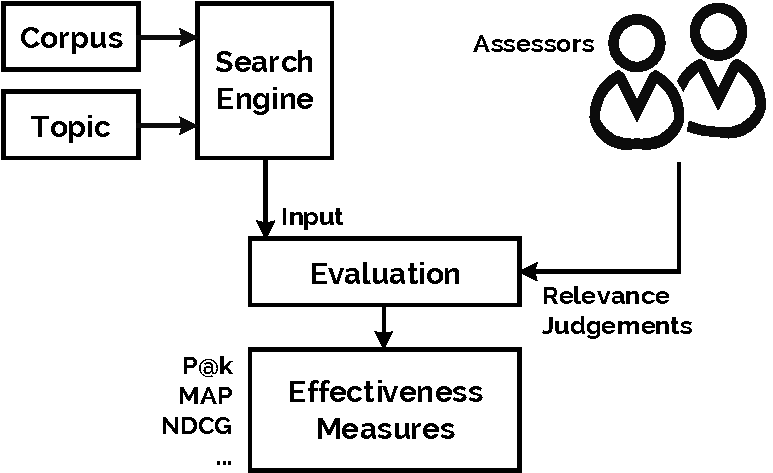
\includegraphics[width=\linewidth]{figures/cranfield.pdf}
% %     \caption{The Cranfield Paradigm. Document collections (corpora) and associated topics are created, and are then passed to assessors to judge the relevancy of documents against the provided topics. These judgements are then provided to researchers as \emph{relevance judgements}, which are then used to evaluate the performance of retrieval components with different \emph{effectiveness measures}, such as \boldmath{$P@k$}.}
% %     \label{fig:cranfield}
% %     \end{center}
% % \end{figure}
% %
% % \subsection{Why Simulation?}
% % A question that readers of this thesis may ask early on is: \emph{why use simulation?} Could the behaviours exhibited by human searchers instead be perhaps modelled through less computationally intensive means? This is a perfectly valid question to ask; indeed, the author tripped up when asked this question at the 1\textsuperscript{st} ACM CHIIR Doctoral Consortium.
% %
% % One of the potential criticisms of this work is: why simulate at all? Why not just plug everything into an equation, and solve it? \url{https://www.cise.ufl.edu/~fishwick/introsim/node2.html}
% %
% %
% % \section{Thesis Statement}
% %
% % - statement of fact: users are complex, and adapt their behaviour due to a variety of different factors, not limited to the ranked list of results presented to them.
% % - statement of fact: many of the models and measures that we use in IR do not assume this.
% % - one thing we do not consider much is stopping behaviour. by incorporating stopping behaviour into our models, we can provide better approximations of searcher behaviour
% %
% % - The statement of this thesis is that incorporating stopping level decision points into a user model will lead to more efficient searching, and better approximations of actual searcher behaviour
% %
% %
% % The statement of this thesis is that we can improve our understanding of the stopping behaviour of searchers through experimentation. This understanding can be further improved through the use of simulation.
% %
% %
% % \section{Overarching Research Questions}
% % From the introductory remarks, thesis statement and motivation as described above, we can now formulate the three main research questions that will be addressed in this thesis.
% %
% % \begin{itemize}
% %
% %     \item[]{\blueboxbold{RQ1} How can we improve upon and make \emph{more realistic models} of the~\gls{acr:iir} search process -- as a whole?}
% %
% %     \item[]{\blueboxbold{RQ2} How can we operationalise and subsequently implement more realistic stopping strategies for use within many of the commonly used~\gls{acr:ir} and~\gls{acr:iir} models and measures that are in use today?}
% %
% %     \item[]{\blueboxbold{RQ3} How do the real-world stopping behaviours of searchers vary under different contexts?}
% %
% % \end{itemize}
% %
% % Each of these research questions will be addressed in parts \blueboxbold{I} and \blueboxbold{II}.
% %
% % \section{Contributions}
% % The work undertaken towards completion of this thesis has led to a number of contributions to the field, many of which have been published in international conference proceedings. The following contributions have been made.
% %
% % \begin{itemize}
% %
% %     \item{An extensible simulator framework, called \emph{SimIIR}, that allows for full-session~\gls{acr:iir} simulation.}
% %
% %     \item{The introduction and evolution of the Complex Searcher Model, a full-session model of the~\gls{acr:iir} process. Note that this model does not attempt to model the brain; rather, it is a model of the overarching steps and decisions that a searcher makes during the search process. We do model state; this does not consider the brain, nor does the model consider other issues such as environmental factors.}
% %
% %     \item{A series of user studies that examine the effects of stopping behaviour on:}
% %
% %     \begin{itemize}
% %         \item{temporal delays;}
% %         \item{snippet lengths; and}
% %         \item{novelty and diversity of results.}
% %     \end{itemize}
% %
% % \end{itemize}
% %
% % \section{Outline}
% % This thesis is split into four logical parts, each of which constitutes a number of chapters.
% %
% % \begin{itemize}
% %
% %     \item{The remainder of \blueboxbold{Part I} provides background of the areas of Information Retrieval and simulation.}
% %
% %     \item{\blueboxbold{Part II} considers the approaches taken to develop the models of IIR further, introducing the Complex Searcher Model.}
% %
% %     \item{\blueboxbold{Part III} examines stopping behaviours, heuristics and strategies in detail, and how the behaviours of searchers is affected by various contexts.}
% %
% %     \item{Finally, \blueboxbold{Part IV} provides conclusions and future work.}
% %
% % \end{itemize}
%
% % --------------------------------
% % -------- NOV 28 BELOW ----------
% % --------------------------------
%
% % We live today in the so-called \emph{Information Age}, an era defined by the creation, transmission, management and \emph{retrieval} of information\footnote{\url{https://en.oxforddictionaries.com/definition/information_age} -- accessed November 26\textsuperscript{th}, 2017.}. With a steady incoming stream of e-mails, articles, and the near-instant reporting of events taking place all around the planet, one would be hard pressed to deny such a claim. Of course, none of this would be possible without the modern-day computer, a now ubiquitous device that can be found in a variety of different shapes and sizes (or \emph{form factors}). Nor would this be possible without the developments of the fundamental technologies that allow for communication between computers, such as the \emph{Internet} -- and associated technologies such as the~\gls{acr:www}~\citep{berners1994www}. Indeed, with technologies today allowing access to the Internet so commonplace, a recent \emph{IBM} technical report estimated that we generate something in the range of \emph{2.5 quintillion bytes} of information \emph{per day}\footnote{$2.5$ quintillion bytes = $2,500,000,000,000,000,000$ bytes, or $2,500,000$ terabytes.}.
% %
% % Sifting through such quantities of information has been a major research challenge, and the field of~\gls{acr:ir}~\citep{rijsbergen1979ir} has existed for several decades. Researchers began with the development
%
%
%
% % explanation of JumpStation~\citep{mcbryan1994taming_tools}
% %
% %
% % We live today in an age of information ubiquity. A constant barrage of e-mails, articles and webpages. A continuous stream of messages on social media platforms. Thanks to the development of the modern computer -- including its various form factors, like the smartphone -- the Internet and the subsequent technologies that have been developed on these key technological advancements -- such as the~\gls{acr:www}~\citep{berners1994www}, we now, according to an IBM technical report\footnote{\url{https://www-01.ibm.com/common/ssi/cgi-bin/ssialias?htmlfid=WRL12345USEN} -- last accessed November 23\textsuperscript{rd}, 2017.}, generate something in the range of 2.5 quintillion bytes\footnote{$2.5$ quintillion bytes = $2,500,000,000,000,000,000$ bytes} of information \emph{per day}.
% %
% % Since the invention of the World Wide Web at CERN in 1989, the \emph{de facto} approach to finding documents within the web of hyperlink documents has been the \emph{search engine}. Search engine technology, although analogous to web search, has been around for much longer -- and contemporary search engines that we use today on a daily basis such as \emph{Google} and \emph{Bing} are considered to offer an effective means of finding the proverbial needle in the haystack.
% %
% % \begin{quote}
% %     ``...but perhaps the key technology that took the Web from a useful supplement of current information practice to become the default communication medium is search.''
% %     \attrib{\citealp{wilson2010keyword_search}}
% % \end{quote}
% %
% % What, however, is the proverbial \emph{needle}? Much work has been undertaken in the field of~\gls{acr:iir} to ascertain and understand the needs of users of search engines. Searchers typically arrive at a search engine in an \emph{Anomalous State of Knowledge (ASK)}~\citep{belkin1980ask}, converting this need into some form of query formulation. The search engine then presents a series of documents to the searcher.
%
%
%
% % \begin{quote}
% %     ``When I first moved into the White House with President Bill Clinton in 1993, there were only 50 existing websites on the World Wide Web.''
% %     \attrib{Al Gore}
% % \end{quote}
%
% % - we live today in an information orientated world.
% % - we need to find information instantly.
% % - volume of information has increased massively.
% % - rate of information generation is remarkable.
% % - thanks to computers and the internet
% % - development of technologies lying upon internet infrastructure, such as the WWW have been key drivers in this development.
% % - 2.5 quintillion bytes of information created on a daily basis.
% %
% % - sifting through all of this information is obviously required.
% % - so the need to search has become paramount and key to our daily lives.
% % - finding the proverbial needle in a haystack is not easy - decades of work have led to this point.
% %
% % - originally, directory-based systems.
% % - but as information grew, so too did the need for search.
% %
% %     \begin{quote}
% %         \Large
% %         ``But perhaps the key technology that took the Web from a useful supplement of current information practice to become the default communication medium is search.''
% %         \attrib{Max Wilson}
% %     \end{quote}
% %
% % - indeed, what is the needle?
% % - searcher arrives in a anomouls state of knowledge.
% % - typically, a searcher will convert this need into some query formulation, and is presented with a series of documents.
% % - this is in essence how a retrieval system works.
% %
% % -
%
%
%
%
% % - as the volume of information that we create has increased, so too has our need to find the information that we need.
% %
% %
% % A searcher approaches an Information Retrieval (IR) system with a need for information derived from an ‘anomalous state of knowledge’ (Belkin et al., 1982). This need is typically transformed into a query statement, submitted to the system and a set of potentially relevant documents is retrieved and presented. The transformation of this need into a search expression, or query, is known as query formulation. Through such transformations and further interaction searchers can conduct Interactive IR (IIR), where they engage in dialogue with the IR system and it dynamically responds to their feedback (Borlund, 2003).
% %
% %
% % Arguably one of the most important developments of the mid-1990's was the introduction of the~\gls{acr:www}.
% %
% % Without it, there is no Google. Without it, there is no Facebook, or any of the other online services that keep the needs of billions satisfied (or perhaps even dissatisfied).
% %
% % The advancement of the~\gls{acr:www}~\citep{berners1994www}...
% %
% %
% % Computers advancement in our age
% % Since the advent of the World Wide Web in the mid-1990's, the amount of information that we generate as humans is estimated to be in the range of 2.5petabytes per day.
% %
% % the rate of information that we generate is remarkable.
% % we create 2.5 quintillion bytes of data per day.
% % 90 percent of all data created by man has been generated in the past few years.
% %
% % \footnote{https://www-01.ibm.com/common/ssi/cgi-bin/ssialias?htmlfid=WRL12345USEN}
% % \footnote{$2.5$ quintillion = $2,500,000,000,000,000,000$ bytes}
    %!TEX TS-program = xelatex
%!TEX root = ../../maxwell2018thesis.tex

% Mention stochastic simulations...

\chapter[Information Retrieval]{Information Retrieval:\\A History and Background}\label{chap:ir_background}
It may be fair to say that \emph{searching for information} is now a commonplace activity within our daily lives. Given the familiarity and near ubiquity of the search box (as shown below) on contemporary human-computer interfaces, one may be forgiven into na\"{i}vely thinking that research and development into the underlying \emph{search engine} that one interacts with when using the search box was focused exclusively upon the domain of \emph{web search}, where names like \emph{Google}, \emph{Bing} and \emph{AltaVista}\footnote{This name might spring to mind for those with more of a historical knowledge of search engines. The author of this thesis has very vague memories using AltaVista when he was around eight years old\dots} spring to mind. Despite potential negatives that these technologies may bring -- turning us into so-called \emph{shallow thinkers}~\citep{carr2008google_stupid}, for example -- search engines today by and large make our lives easier, allowing us to find that proverbial needle in the haystack with relative ease.

\begin{figure}[h]
    \centering
    \vspace{4mm}
    \resizebox{1\hsize}{!}{
    
\includegraphics{figures/ch2-searchbox.pdf}}
    \label{fig:searchbox}
    \vspace{-5mm}
\end{figure}

The research and development that has gone into search and indexing technologies that allow us to find that proverbial needle has been going on for decades, long before the advent of computers and associated communication technologies, such as the~\gls{acr:www}. This research has led to the formation of the study of~\gls{acr:ir} and the development of contemporary~\gls{acr:ir} systems.\footnote{Some within the~\gls{acr:ir} may consider this to be a contentious point: does the~\gls{acr:ir} community embrace those wishing to contribute? One of the most famous research papers associated with~\gls{acr:ir} discussing Google's \emph{PageRank} algorithm~\citep{page1998pagerank}, was rejected from SIGIR. See \url{http://rakaposhi.eas.asu.edu/f08-cse494-mailarchive/msg00037.html} (last accessed March 6\textsuperscript{th}, 2018) for more information.} With this field of study has come with it the development a \emph{de facto} approach to conducting~\gls{acr:ir} research, along with various retrieval models and means with which to evaluate their effectiveness. It is in this vain that we frame this chapter: beginning with a brief history of~\gls{acr:ir} research (Section~\ref{sec:ir_background:history}), we then consider the basic assumptions and approaches used within the field for experimental research (Section~\ref{sec:ir_background:basics}) and how we evaluate these experiments (Section~\ref{sec:ir_background:evaluation}).

\section{A (Brief) History of Information Retrieval}\label{sec:ir_background:history}
It has only been over the last two decades that search engines have become commonplace in our daily lives, primarily for the domain of web search -- as discussed in Section~\ref{sec:ir_background:history:www}. Contemporary search technologies are essentially ubiquitous, integrating seamlessly with computer operating systems (as illustrated in Figure~\ref{fig:search_integration}). Computerised~\gls{acr:ir} systems have however existed as far back as the late 1940's (as demonstrated by~\citealp{holmstrom1948univac}), with more primitive approaches (both mechanised and manual categorisation approaches) to sorting and categorising information being developed even earlier.

\begin{figure}[t!]
    \centering
    \resizebox{1\hsize}{!}{
    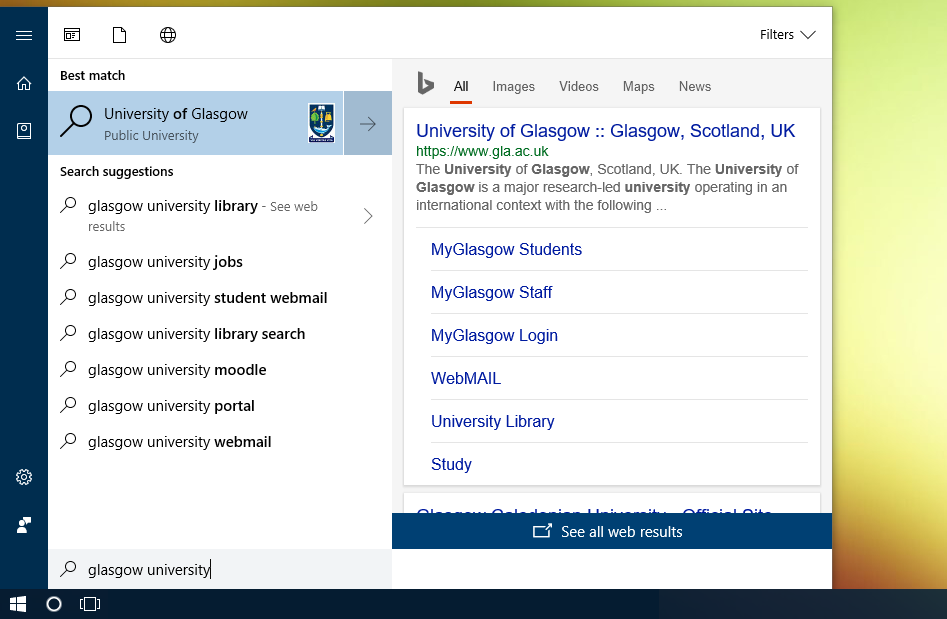
\includegraphics{figures/ch2-search_integration.png}}
    \caption[Search Integration within Windows\textregistered~10]{An example of search integration within the Windows\textregistered~10 operating system. Here, results for the query \texttt{glasgow university} are shown. Results are returned from the \emph{Bing} search engine; one can also search for files on their local computer.}
    \label{fig:search_integration}
\end{figure}

\subsection{Libraries and Mechanisation}
Before the advent of computers and technologies such as the~\gls{acr:www}, one of the first locations in which one would consult when looking for information would be a \emph{library}. Containing a large volume of books discussing a virtually unlimited range of categories, the need for providing a means to organise (and thus locate) information with relative ease was of paramount importance. \emph{Catalogues} provide such a way in which to do this, with ancient Greek poet Callimachus being the first person to create such an item, in the third century BC~\citep{eliot2009companion}. A more recognisable approach to categorising content was devised by~\cite{dewey1891dcs} with the \emph{Dewey Decimal System}. The use of cards as an \emph{indexing system} was also considered by individuals such as~\cite{soper1920patent} who invented a system of providing information on what category a card belonged to based upon a punched hole.

In order to speed up the process of finding useful material, mechanisation was also extensively used. Allowing for searching at the rate of 600 cards per minute, Luhn devised in the early 1950's a mechanised system which utilised punchcards and light. As stated by~\cite{sanderson2012history_of_ir}, this was also around the time that the term~\glsfirst{acr:ir} was used~\citep{mooers1950theory}. It was at this point that computer technology was rapidly developing as a base for a viable, faster alternative to manual and mechanised approaches. This therefore led to the demise of mechanised systems, as highlighted by~\cite{jahoda1961electronic_searching}.

\subsection{The Rise of Computers}
Computers today provide the medium with which we closely associate a typical~\gls{acr:ir} system.~\cite{sanderson2012history_of_ir} state that digital storage capacity (e.g. hard disks) roughly doubles every two years -- similar to the famous \emph{Moore's Law}~\citep{moore1965law}, which observes that the number of transistors in a processor (or integrated circuit) doubles roughly every two years. Indeed, the speed at which contemporary computers can search vast indexes and databases of content is vastly superior to traditional cataloguing approaches.

One of the earliest discussions about the use of computers as the basis for an~\gls{acr:ir} system specifically mentioned the~\gls{acr:univac}.~\cite{holmstrom1948univac} described a (potentially pre-production)~\gls{acr:univac} system that was capable of searching for text with a given \emph{reference code} stored on steel tape.~\cite{mitchell1953univac_million} also showed a~\gls{acr:univac} system capable of searching one million records indexed by six subject codes. It was around this time that computers began to replace the traditional librarian, being able to provide a much more effective and cost effective means of trawling through a library's records.

From this point on, work began to establish~\gls{acr:ir} as a scientific field. Gerard Salton established a large~\gls{acr:ir} research group, initially at Harvard University. Many of the basic constructs which we utilise within~\gls{acr:ir} today were established around this time, in addition to the experiments undertaken by~\cite{cleverdon1962cranfield_experiments} -- known as the \emph{Cranfield Experiments}. These experiments established the concept of using words to index documents within an~\gls{acr:ir} system, providing advancements in indexing technology.~\cite{luhn1957ranking_query} proposed, and~\cite{maron1959probabilistic_indexing} tested, an approach to ranking that scored documents in a collection in relation to a user issued \emph{query} -- a concept that is central to contemporary~\gls{acr:ir} systems. A detailed explanation of these concepts are provided later in this chapter -- refer to Section~\ref{sec:ir_background:basics}.

\begin{figure}[t!]
    \centering
    \resizebox{1\hsize}{!}{
    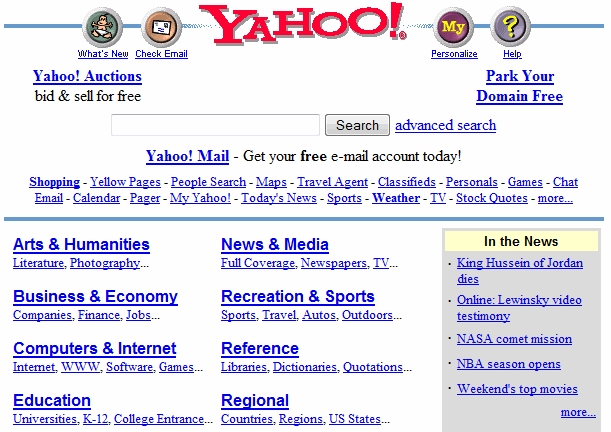
\includegraphics{figures/ch2-yahoo.png}}
    \caption[Screenshot of \emph{Yahoo!} Search, July 1998]{A screenshot of the landing page of \emph{Yahoo!}, as shown on July 5\textsuperscript{th}, 1998. Notice the link for the 1998 \emph{FIFA World Cup} that was taking place at the time the page was created. More central to this thesis is the inclusion of a list of page categories in conjunction with the now ubiquitous search box. Screenshot acquired from the \href{https://web.archive.org/web/19980705003104/http://www.yahoo.com}{\emph{Internet Archive}}.}
    \label{fig:yahoo}
\end{figure}


\subsection{The World Wide Web}\label{sec:ir_background:history:www}
The distribution and ability to search for information over computer networks such as the internet was traditionally undertaken with legacy protocols such as \emph{Gopher}. Gopher would provide a series of options for a user to select (i.e. categorisation), akin to the traditional library cataloguing approaches described above.

The advent of the~\gls{acr:www} in the early 1990's brought about a new type of search engine -- \emph{web search engines}. Regarded as the first experimental web search engine, \emph{JumpStation} was described by~\cite{mcbryan1994taming_tools}. In this system, \emph{anchor text} within \emph{hyperlinks} of~\gls{acr:html} pages could be exploited to aid the ranking of documents. However, popular search engines of the 1990's initially followed the categorisation approach hailing back from libraries, as illustrated in Figure~\ref{fig:yahoo} with a screenshot of \emph{Yahoo!} from 1998. However, as the volume of information on the~\gls{acr:www} began to increase, this approach became impractical. As such, it was not long before a more contemporary search engine took ahold, with the search box, allowing searchers to pose their own \emph{queries}, becoming the dominant (and defining) symbol of search. Algorithms such as Google's PageRank~\citep{page1998pagerank} took hold, with this algorithm credited for cementing Google's dominance of the search market. Over the past two decades, there have been many advances from these initial approaches to developing~\gls{acr:ir} systems. For example, the exploitation of interaction logs have become commonplace in search engines to assist in providing higher quality results, and a more personable experience for searchers.

\section{Information Retrieval Basics}\label{sec:ir_background:basics}
As already has been explained in Chapter~\ref{chap:intro}, the key purpose of an~\gls{acr:ir} system is to locate information that is relevant to a searcher's \emph{information need.}\footnote{To recap, an information need can be considered as a desire to locate and obtain information that satisfies some conscious or unconscious need~\citep{hjorland1997information}.} Such a system would search through collection(s) of \emph{unstructured} or \emph{semi-structured} data (such as a collection of web pages, documents, images, videos, etc.), before returning potential matches to the searcher. 

\blueboxheader{Unstructured vs. (Semi-)Structured Data}
A key difference between~\gls{acr:rdbms} and~\gls{acr:ir} systems is the type of data that they both consider. While  a~\gls{acr:rdbms} considers \emph{structured data,} an~\gls{acr:ir} system in contrast considers \emph{(semi-)structured data} (refer to Figure~\ref{fig:structured_data}). With an~\gls{acr:ir} system, such a premise for structured data does not exist.\footnote{This may be a slight misnomer; schemas can be used for an~\gls{acr:ir} system index when considering \emph{fielded retrieval}. For example, a collection of newspaper articles may contain a title and body -- but within the fields, the data is unstructured.} Semi-structured data such as an~\gls{acr:html} page contains a series of \emph{elements} (e.g. \texttt{<h1>} for headers), but the text within these tags is largely of an unstructured nature. The unstructured data can contain information such as dates or entities (terms describing a real-world object and/or location, such as \texttt{canberra} or \texttt{dropbear}, and can be -- as it is probably written in a natural language -- ambiguous. As such, unstructured data presents a major challenge to address, and is the cornerstone of~\gls{acr:ir} research.

\begin{figure}[t!]
    \centering
    \resizebox{1\hsize}{!}{
    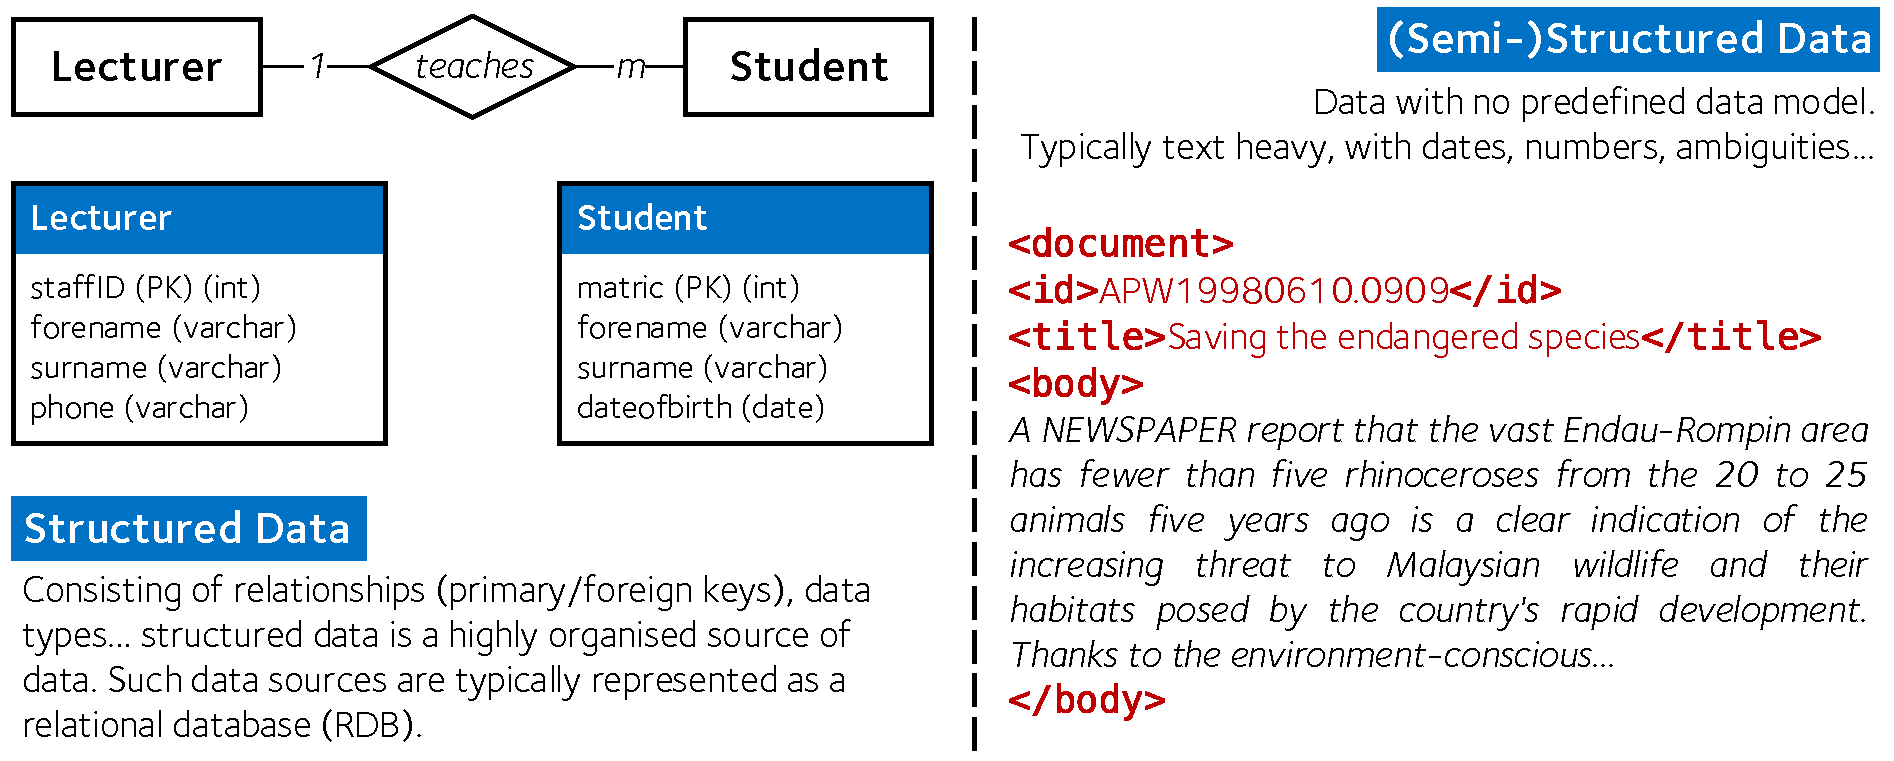
\includegraphics{figures/ch2-structured.pdf}}
    \caption[Structured and (semi-)structured data]{Examples of structured and (semi-)structured data. On the left is a structured~\gls{acr:rdbms} schema, represented in compressed Chen notation. Different types can be specified for each field, representing data in a structured way. On the right, semi-structured data, using a document from the \emph{TREC AQUAINT} newswire collection. Note the semi-structured component at the top of the document (containing an identifier and title), and the unstructured body text.}
    \label{fig:structured_data}
\end{figure}

To complement this challenge, a contemporary~\gls{acr:ir} system is also expected by its users to return results that can be considered \emph{useful} to addressing the searcher's information need, as hypothesised by~\cite{luhn1957ranking_query}, and succinctly expressed by~\cite{robertson1977prp}.

\begin{quote}
    ``A [reference] retrieval system should rank references in the collection in order of their probability of relevance to the request, or of usefulness to the user, or of satisfying the user.''
    \attrib{\cite{robertson1977prp}}
\end{quote}

\blueboxheader{Search Queries}
A searcher's information need is represented as a \emph{query}. which is in turn comprised of one or more salient \emph{query terms}. The process of converting an information need to a query is known as \emph{query formulation}~\citep{hiemstra2009ir_models}. Depending upon the search domain, the query language used may be artificial. For example, reserved keywords may be utilised to express a \emph{boolean query} (e.g. use of \texttt{AND} or \texttt{NOT} preceding terms -- refer to Section~\ref{sec:ir_background:basics:models:boolean} for more information). Natural language however is considered to be the preferred choice within an~\gls{acr:ir} context~\citep{rijsbergen1979ir}. Given the claim by~\cite{robertson1977prp} above, an~\gls{acr:ir} system then typically returns a series of documents.

\blueboxheader{Results}
Depending upon the type of retrieval system used, these results may be ranked in order of decreasing perceived relevance via some form of \emph{retrieval model.} We discuss the basic families of retrieval model in Section~\ref{sec:ir_background:basics:models}. On contemporary~\gls{acr:ir} systems, results are typically presented on a~\glsfirst{acr:serp}, complete with the \emph{ten blue links}~\citep{hearst2009_search}. This name is given to the way in which retrieval systems typically present results to searchers. If none of the results returned to the searcher can be considered useful in addressing his or her information, the underlying~\gls{acr:ir} system can be said to have failed the searcher~\citep{rijsbergen1979ir}. Of course, this is something commercial retrieval engines attempt to avoid -- perhaps through the use of strategies such as \emph{diversification} of results -- producing a series of unsatisfactory results will simply mean searchers move elsewhere, costing the business revenue.

\begin{figure}[t!]
    \centering
    \resizebox{1\hsize}{!}{
    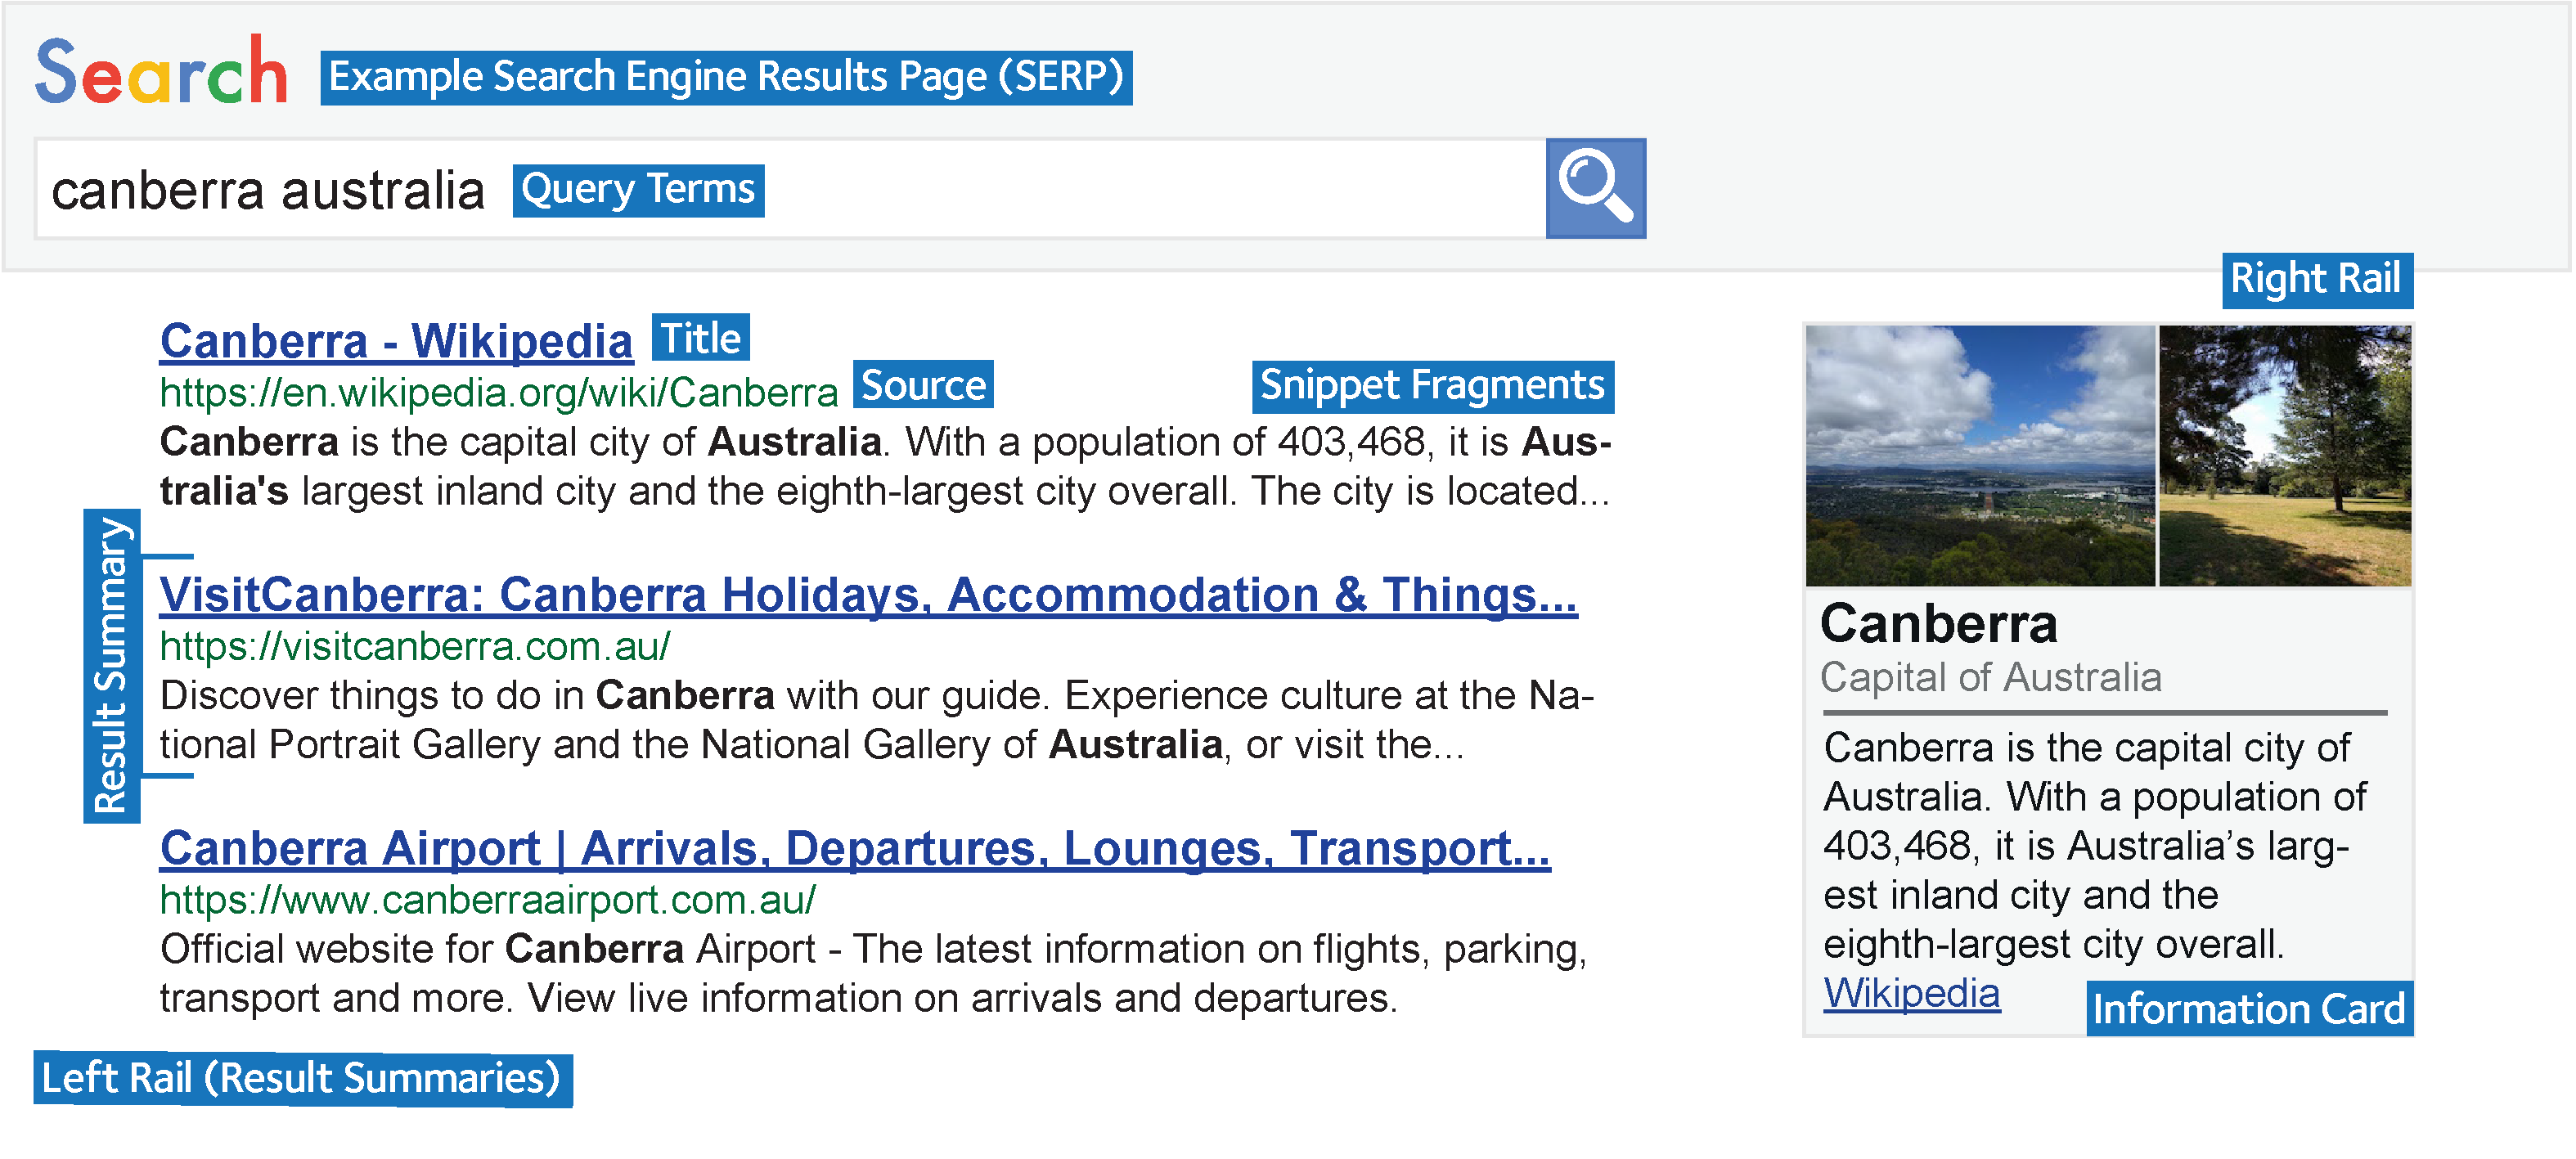
\includegraphics{figures/ch2-example.pdf}}
    \caption[Example of a~\gls{acr:serp}]{An example of a~\glsfirst{acr:serp} for the query \texttt{canberra australia}. \blueboxbold{Labels} illustrate the names of the key components of a~\gls{acr:serp} -- of particular relevance for the work in this thesis are the \emph{verticals,} consisting of one or more \emph{result summaries.}}
    \label{fig:serp_example}
\end{figure}

\blueboxheader{Presenting the~\gls{acr:serp}}
As previously mentioned, results are typically presented on the so-called~\glsfirst{acr:serp}. Figure~\ref{fig:serp_example} depicts an example~\gls{acr:serp} of fictional retrieval system, \searchlogo.\footnote{We utilise \searchlogo~throughout this thesis to illustrate various techniques and approaches.} The illustration highlights several key areas of~\gls{acr:serp} components that we briefly discuss here. At the top of the~\gls{acr:serp} is the \blueboxbold{query box}, allowing for a searcher to enter a new query if he or she desires. This is typically referred to as \emph{query (re)formulation} in the literature. The main body of the~\gls{acr:serp} is then divided up into the \blueboxbold{left rail} and \blueboxbold{right rail}.

\begin{itemize}
    
    \item{The \blueboxbold{left rail} of the~\gls{acr:serp} contains the traditional \emph{ten blue links}~\citep{hearst2009_search}, or \emph{verticals.} While contemporary~\glsplural{acr:serp} contain different types of media (e.g. images), we assume for the work in this thesis that the verticals consists purely of traditional, textual \blueboxbold{result summaries}. In this work, a result summary, as illustrated in Figure~\ref{fig:serp_example}, consists of three main components:}
    
    \begin{itemize}
        \item{a \blueboxbold{title} that represents the title, or headline, or a source object;}
        \item{one or more \blueboxbold{textual snippets}, providing a summary of the source object such that searchers can determine whether it is worth examining the result in more detail or not; and}
        \item{a \blueboxbold{source} for the object, typically an~\gls{acr:url} if the object is~\gls{acr:www}-based.}
    \end{itemize}
    
    \item[]{Snippets are of particular interest to the work in this thesis; we explore the effect of their length on stopping behaviour in Chapter~\ref{chap:snippets}. Snippets are typically presented in contemporary retrieval systems as \emph{query-biased}~\citep{tombros1998query_biased}. This means that the snippet text relates to terms that were present in the searcher's query. Figure~\ref{fig:serp_example} demonstrates this with the use of \textbf{bolded} terms in example snippet text.}
    
    \item{The \blueboxbold{right rail} is relatively recent development in~\gls{acr:serp} presentation, typically containing information to supplement the presented verticals on the left rail. The example illustrated in Figure~\ref{fig:serp_example} provides an \emph{information card,} presenting images and basic facts about the city of Canberra, ACT, Australia. Work has been undertaken examining the effects on searchers that these additional, contemporary components bring to the table -- refer to~\cite{bota2016information_cards} for an example of such work.}
    
\end{itemize}

While the introduction of the~\gls{acr:serp} deviates slightly from the narrative of this chapter, it is nevertheless important to introduce the names of the various~\gls{acr:serp} components used. We make extensive use of these terms throughout the remainder of this chapter, and indeed throughout the remainder of this thesis. For the purposes of this work, we consider~\glsplural{acr:serp} to be presented \emph{without} contemporary right rail components, such as the information card. As such, a~\gls{acr:serp} consists purely of the left rail verticals, containing one or more result summaries for the searcher to examine for relevance.

\blueboxheader{Operational and Experimental Systems}
\cite{rijsbergen1979ir} defines a difference between \emph{operational} and \emph{experimental}~\gls{acr:ir} systems. While a majority of individuals will only ever interact with an operational, probably commercial~\gls{acr:ir} system (e.g. Google), the work described in this thesis considers purely experimental systems. In order for one to determine how well a particular experimental~\gls{acr:ir} system performs compared to others, a rigid scientific methodology must be employed to allow for fair comparisons. As such, the remainder of this chapter discusses the \emph{de facto} approach that is considered for~\gls{acr:ir} experimentation -- from the setup of such an~\gls{acr:ir} system to the ways in which they can be evaluated.

\subsection{The Cranfield Model}\label{sec:ir_background:basics:cranfield}
The methodology behind the majority of contemporary~\gls{acr:ir} research has centred around the concept of the so-called \emph{Cranfield Model}. Devised, unsurprisingly, at Cranfield University in Bedfordshire, England, the model is based upon the \emph{Cranfield II} experiments~\citep{aslib1966factors}. As highlighted by~\cite{borlund2003iir_model}, the experiments revolve around the notion of \emph{test collections}, with the basic components of the experimental setup illustrated in Figure~\ref{fig:ir_cranfield}. Essentially, the concept of test collections is comprised of three main components.

\begin{itemize}
    \item{A collection of \emph{documents} is provided, which is typically converted to an inverted index before experimentation can begin (refer to Section~\ref{sec:ir_background:basics:indexing}).}
    \item{A collection of \emph{topics} provide a means of simulating different information needs -- and with each topic are one or more \emph{queries} that can be issued to an experimental~\gls{acr:ir} system.}
    \item{Finally, a collection of \emph{relevance assessments} are provided as part of the collection.}
\end{itemize}

\begin{figure}[t!]
    \centering
    \resizebox{1\hsize}{!}{
    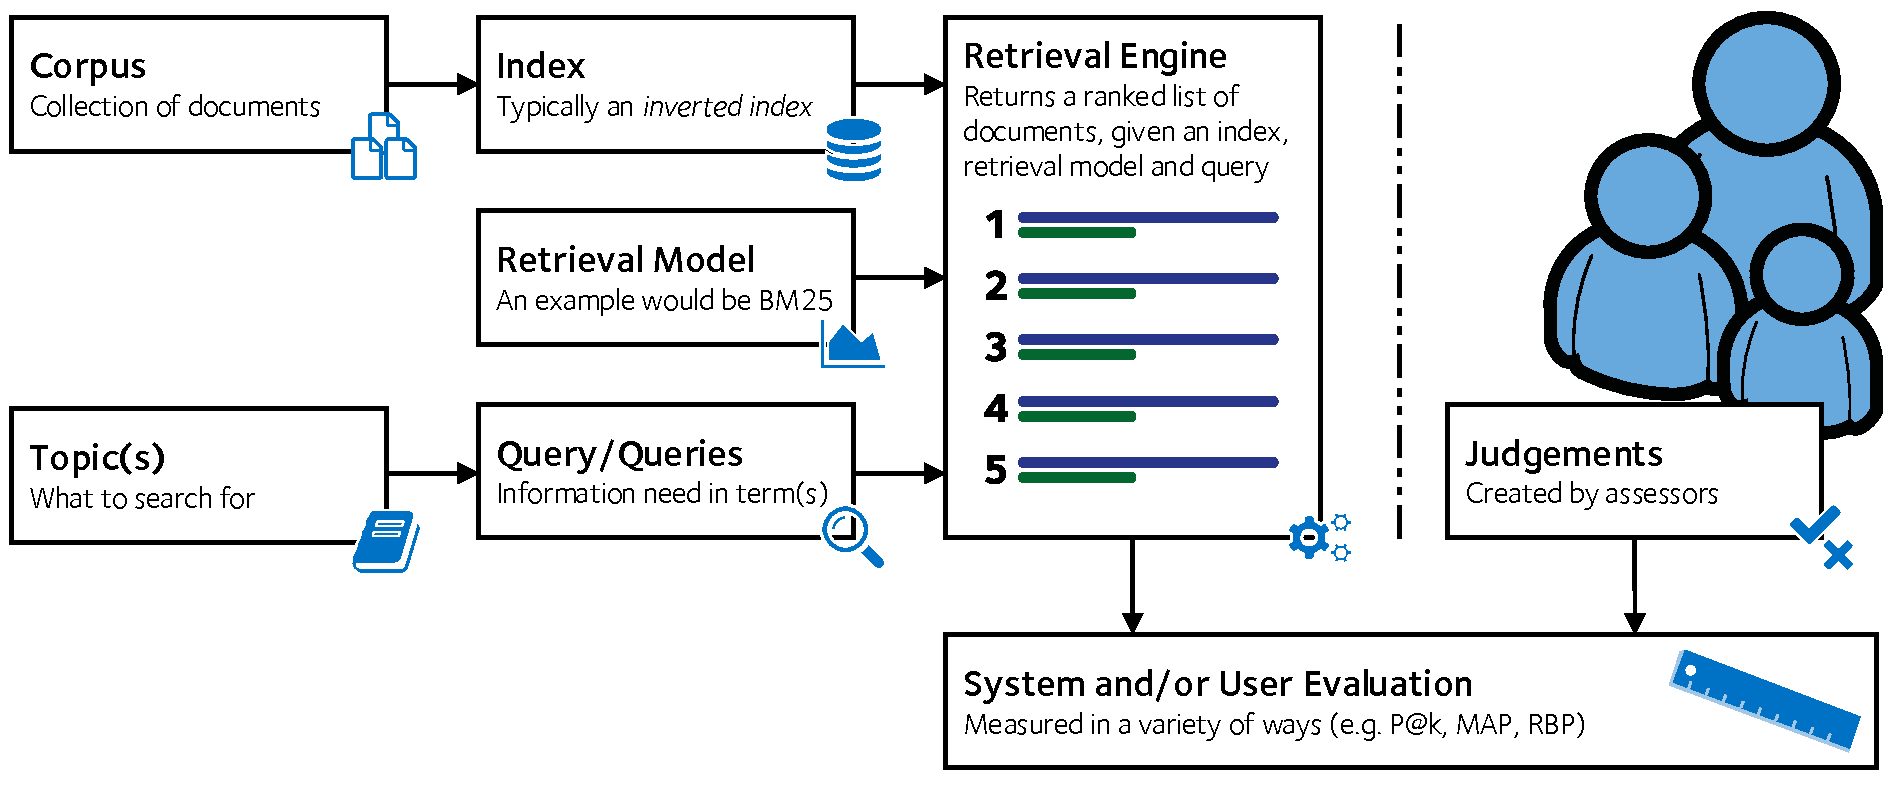
\includegraphics{figures/ch2-cranfield.pdf}}
    \caption[The \emph{Cranfield Model}]{Illustration of the Cranfield Model, the \emph{de facto} approach experimental methodology used for~\gls{acr:ir} research. Given a corpus, topic(s) and document judgements (created by assessors), one can compute various evaluation measures for a given retrieval model and search engine.}
    \label{fig:ir_cranfield}
\end{figure}

In conjunction with the documents and topics, a \emph{retrieval model} is employed (refer to Section~\ref{sec:ir_background:basics:models}), which encapsulates our beliefs about the nature of what constitutes \emph{useful} content. When instantiated, these components are in turn used by the \emph{retrieval engine} to produce a list of potentially useful documents -- called the \emph{matching process}. Many experimental retrieval engines exist, with a non-exhaustive list including: the \emph{Terrier~\gls{acr:ir} platform}\footnote{\url{http://terrier.org/}}; \emph{Apache Lucene}\footnote{\url{https://lucene.apache.org/}}; and \emph{Whoosh}\footnote{\url{https://pypi.python.org/pypi/Whoosh/} -- all URLs mentioned in this footnote were last accessed on March 8\textsuperscript{th}, 2018. \todo{Check they are all on the same page.}}. A specific retrieval engine can be selected based upon the requirements and existing infrastructure available for the particular experiment. In this thesis, for example, we rely upon the Whoosh retrieval engine for all experimental work. Output from the experimental system can then be evaluated using an \emph{evaluation tool} to produce a series of measures to examine the performance of the system (refer to Section~\ref{sec:ir_background:evaluation}).

Relevance assessments are created for each topic of the collection. Assessors examine a series of documents that are extracted from the document collection using a simple query (called \emph{pooling}). For example, given a topic \texttt{wildlife extinction}, a query typically issued to retrieve documents will also be \texttt{wildlife extinction}. The returned documents are then assessed for relevance to the given topic, and a judgement is assigned to each. Typically, such a judgement has been binary, with \texttt{0} denoting non-relevant, and \texttt{1} denoting relevant. The effects of pooling can mean that documents that are potentially relevant can be missed by assessors, and thus will receive no judgement~\citep{keenan2001effect}.

\subsubsection{The Text REtrieval Conference}\label{sec:ir_background:basics:cranfield:trec}
A number of different evaluation forums have been borne out of the Cranfield model. Perhaps most notably is~\gls{acr:trec}, as sponsored by the U.S. Government funded \emph{National Institute for Standards and Technology (NIST)}. Other efforts which have been inspired by~\gls{acr:trec} include \emph{NTCIR}, \emph{CLEF} and \emph{INEX}. Experimentation following the original~\gls{acr:trec} approach is named\emph{~\gls{acr:trec}-style} in this thesis.

Originally organised by Donna Harman and Ellen Voorhees,~\gls{acr:trec} provides a platform for annual collaboration between research groups interested in different aspects of~\gls{acr:ir} research. Each year, a series of~\gls{acr:trec} \emph{tracks} are defined, with each consisting of a collection of documents, topics and relevance judgements. Those who provide the judgements are assessors, usually employees of NIST~\citep{robertson2008history_ir_evaluation}, who were in turn previously employed as news analysts by various U.S. security agencies. Each team wishing to participate in a track receives the collection, and runs them through their experimental search system, following the approach illustrated in Figure~\ref{fig:ir_cranfield}.

Output from the experiments should then be produced in a standardised format. Results can then be used in conjunction with the judgements (termed \emph{Query RELevance judgements}, or \emph{QRELs}), again, as illustrated in Figure~\ref{fig:ir_cranfield}, and fed into a standardised program called \texttt{trec\_eval}\footnote{\texttt{trec\_eval} is downloadable from \url{http://trec.nist.gov/trec_eval/} -- URL last accessed on March 8\textsuperscript{th}, 2018. Version 8.1 of the software was used for computing most of the evaluation measures reported in this thesis.} to perform evaluation of the runs that are undertaken. The application returns the values for a number of common system-sided evaluation measures, some of which are discussed in Section~\ref{sec:ir_background:evaluation}. 

The collaborative (and perhaps competitive) atmosphere that TREC has fostered has broadly been accepted to be good for the~\gls{acr:ir} community. As discussed by~\cite{robertson2008history_ir_evaluation}, some of the main advantages of~\gls{acr:trec} is that it has encouraged a good, formalised scientific methodology for~\gls{acr:ir}. In addition, the provision of providing the community with a large volume of standardised test materials of the quality and quantity in which~\gls{acr:trec} has done is nothing like what was previously available.~\cite{robertson2008history_ir_evaluation} goes on to claim that simply examining the number of research papers published in the field employing some form of~\gls{acr:trec} data is substantial, and that alone is enough to justify the existence of the forum. Standardised sets should also aid reproducibility of research, although we acknowledge that there are other factors at play in order to achieve that goal. 

As previously mentioned,~\gls{acr:trec} is comprised of a series of different tracks, each with its own set of tasks. Some of the tasks, such as those in the \emph{Interactive Track}, as what as known as \emph{ad-hoc}. This type of task can be considered as one of the most obvious for search, when a searcher develops a need for information, and then issues a query to an underlying search engine. Tasks like ad-hoc essentially provide a form of \emph{user model}, one that has been extensively used within~\gls{acr:ir} research for a number of decades. Section~\ref{sec:stopping_background:models:conceptual:trec} provides more information on the steps involved in the model, and what it assumes.

\noindent
\blueboxbold{A Less Critical Eye} Of course, the work in this thesis cast a critical light over the underlying user model proposed by~\gls{acr:trec}. We understand and appreciate that~\gls{acr:trec} did not necessarily consider the \emph{user} from the beginning, but rather to instantiate a solid evaluation framework. Without the efforts of those who have been involved with~\gls{acr:trec} over the decades, we would not have the test collections, relevance judgements and other infrastructure with which much of the work in this thesis is based upon. To that end, we, along with the entire~\gls{acr:ir} community, owe those who made~\gls{acr:trec} possible a huge debt of gratitude for making \emph{our work possible.}

\subsection{Indexing Documents}\label{sec:ir_background:basics:indexing}
As previously discussed, the conversion of a series of documents (corpus) into a data structure facilitating fast, full-text search -- as required of an~\gls{acr:ir} system -- is known as \emph{indexing}. This full-text searching is undertaken, usually in milliseconds, in aid of finding useful documents for a given query. Without an index, a retrieval engine would have to manually examine each and every document within a corpus. This would require significant computational power -- and is indeed infeasible for a large scale index, such as the index used in a contemporary commercial web search engine. The additional storage space and management required to maintain an index of documents is considered to be a necessary tradeoff to guarantee timely responses to queries.

\begin{figure}[t!]
    \centering
    \resizebox{1\hsize}{!}{
    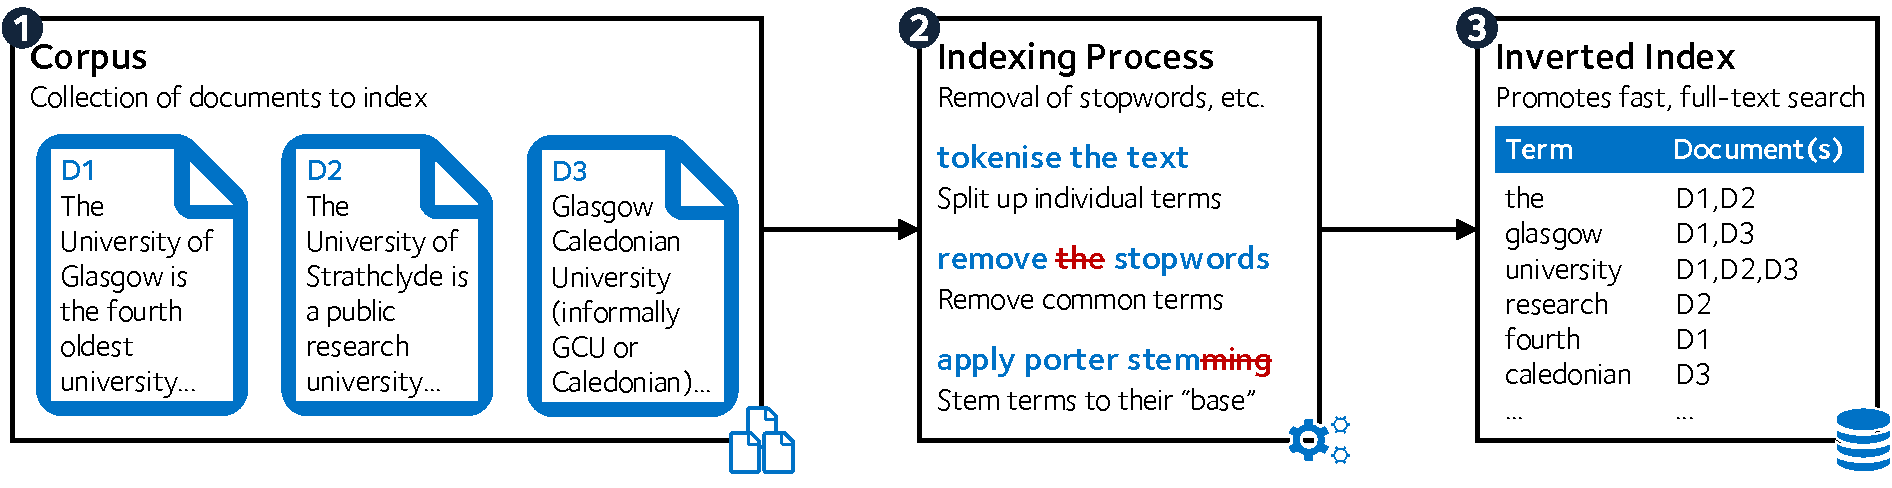
\includegraphics{figures/ch2-inverted.pdf}}
    \caption[Illustration of an \emph{Inverted index}]{A demonstration of an \emph{inverted index}, with three source documents for comparison. Depending upon the requirements of the~\gls{acr:ir} system, the indexing process may vary; all classical~\gls{acr:ir} systems however rely upon some form of inverted index.}
    \label{fig:inverted}
\end{figure}

As illustrated in Figure~\ref{fig:inverted}, the indexing process can be split into three main steps: 

\begin{itemize}
    \item{gathering the corpus of documents to be indexed;}
    \item{performing pre-indexing data preparation; and}
    \item{creating the inverted index.}
\end{itemize}

For the purposes of IR experimentation, most corpora are provided in from the evaluation forum providing the raw materials. As an example, at the time of writing, the University of Glasgow provides the TREC \emph{W2Tg}, \emph{WT10g}, \emph{.GOV} and \emph{.GOV2} document collections.\footnote{Refer to \url{http://ir.dcs.gla.ac.uk/test_collections/} -- URL last accessed March 10\textsuperscript{th}, 2018.}

Running~\gls{acr:ir} experiments with provided test collections is the case for~\gls{acr:ir} experiments following the Cranfield model -- including, of course, TREC experimentation (refer to Section~\ref{sec:ir_background:basics:cranfield:trec}), and the work presented in this thesis. For operational~\gls{acr:ir} systems, data is collated by other means. For example, web search engines employ a \emph{crawler} to examine pages on the~\gls{acr:www} and accumulates more content by following the web's hyperlink structure. Google's crawler for example is called the \emph{Googlebot}, and regularly crawls high impact websites (e.g. popular news sites, such as \emph{BBC News}) to ensure that the associated index is continually refreshed with up to date information. The enormous size of an index that would be employed by Google for web search -- as well as the need for it to be continually updated -- is itself a major engineering challenge, and is not covered in this chapter.

With the indexing process examining each document within the corpora under consideration, a complete \emph{index} will contain an entry for each processed document along with a \emph{vector} of terms that are present within said document. This is known as the \emph{forward index}. An~\gls{acr:ir} system however needs to support fast full-text search, matching terms from a searcher's query to one or more documents within the corpora. To support faster query matching, the most simplistic approach is to \emph{invert} the index, such that the lookup of the index then corresponds to an individual term. A vector of \emph{documents} is then provided for each term, allowing the system much faster access to a potential list of documents. An example of the so-called \emph{inverted index} is provided in Figure~\ref{fig:inverted}. The source corpora in this example illustration contains three documents, and the resultant inverted index is shown. The set of documents retrieved can then be sent to a retrieval model for ranking.

Before a document is indexed however, a number of pre-indexing processes take place on the raw document data as previously mentioned. We now discuss three of the most common processes involved within such a pipeline, including: \emph{tokenisation}, \emph{stopword removal} and \emph{stemming}.

\subsubsection{Tokenisation}
Put simply, tokenisation is the process of \emph{parsing} a source document, and splitting the data within the document into a number of individual \emph{tokens} that may be subsequently indexed. A token is considered a sequence of characters, grouped together to be semantically useful for processing its given document. While we do not go into greater deeper about the process of tokenisation, there are many challenges to this process -- such as \emph{word boundary ambiguity}. While parsing an English or Latin-based document may be relatively straightforward (with spaces representing \emph{word boundaries}), what about other languages, such as Chinese or Japanese? A goal for solving this problem may be to consider what words a potential searcher of an~\gls{acr:ir} system may use to search with in their query.

\subsubsection{Stopword Removal}\label{sec:ir_background:basics:indexing:stopwords}
Stopword removal is another popular choice for indexing document collections for an experimental~\gls{acr:ir} system. Extremely common words which would appear to have little value in selecting documents matching a searcher's query (that is, \emph{non-discriminative} words) can simply be removed from a document's vocabulary entirely. Examples of such words could be \emph{the}, \emph{a}, or \emph{did}. Such words are regarded as \emph{stopwords}. Some experiments consider a small list of stopwords, while others consider a larger list, with larger lists often significantly reducing the size of an indexed corpus~\citep{manning2008ir}. Indeed, it was argued by~\cite{fox1992stopwords} that larger lists ``are advisable''. This was aptly demonstrated by~\cite{dolamic2010stopword}, showing that indexing a with a longer stopword list resulted in significantly improved performance when compared to a much smaller list.

The simplest strategy for producing a list of stopwords would be to count the \emph{term frequency} for each term within a corpus, and sort the list in descending order, selecting some top $k$ of the most frequently occurring terms. Others have produced stopword lists for use in~\gls{acr:ir} research --~\cite{rijsbergen1979ir} produced a list of 250 terms, with~\cite{francis1985stopwords} demonstrating a list of 425 stopwords from the \emph{Brown corpus}\footnote{The \emph{Brown corpus} was a collection of documents representing (then) contemporary American English, compiled by William Francis and Henry Ku\v{c}era -- refer to~\cite{francis1979brown_manual} for more information.}. For the experiments detailed in this thesis, \emph{Fox's classical stopword list}~\citep{fox1992stopwords} is used, consisting of 421 terms. Such an approach may be considered fine, but stopwords lists do vary from collection to collection, as stated by~\cite{lo2005automatically}.

Of course, issues also exist with removing stopwords. For example, what if a searcher issued the query \texttt{to be or not to be}, a phrase from the famous soliloquy of William Shakespeare's \emph{Hamlet?} Such a term could be forgiven to be consisted \emph{entirely} of stopwords. If stopword removal were to be employed, the resultant query to the underlying search engine would contain a grand total of zero terms! As such, commercial search systems are less likely to employ stopword removal~\citep{manning2008ir, dolamic2010stopword} to counter such an issue, employing techniques such as compression to keep the size of the index down. Queries like the one above do contain some meaning -- like tokenisation, there is often more to this problem than meets the eye.

\subsubsection{Stemming}
The final pre-indexing process we consider is \emph{stemming} (also called \emph{lemmatisation}). This is the process of reducing inflected -- or sometimes derived -- words from their \emph{word stem}, \emph{base} or \emph{root}. For example, given the terms \texttt{fisher}, \texttt{fished} and \texttt{fishing}, reducing each of these terms to their respective word stem would result in \texttt{fish}. Essentially, stemming allows one to group words together with a similar, basic meaning. This provides the advantage of reducing the size of an index, and can potentially increase the number of possible matches that can be found with a stemmed set of query terms.

The concept of stemming has been studied since the 1960's, with the \emph{Porter stemmer}~\citep{porter1980algorithm} emerging over time as empirically the most effective.\footnote{The Porter stemming algorithm is not provided in this thesis; refer to~\cite{porter1980algorithm} for an in-depth explanation of the algorithm.} Comprised of a series of linguistic rules, the \emph{measure} of a word can be considered, where \emph{``loosely checking the number of syllables to see whether a word is long enough that it is reasonable to regard the matching portion of a rule as a suffix rather than as part of the stem of the word.''}~\citep{manning2008ir}. Porter stemming is utilised in the indexing process for the work reported in this thesis; other stemmers do exist, such as the original single pass stemmer devised by~\cite{lovins1968development}.

However, issues again exist that must be considered. \emph{Overstemming} is a potential issue, where a word is reduced too far to the point that it loses meaning -- and thus can negatively effect the search results returned. Terms like \texttt{universe}, \texttt{university} and \texttt{universal} when stemmed will be reduced to \texttt{univers}. The three terms are etymologically linked; their modern meanings are however very different. To counter potential issues like this, techniques such as \emph{$n$-grams} may be employed.


\subsection{Retrieval Models}\label{sec:ir_background:basics:models}
In order to achieve the goal of satisfying a searcher's underlying information need, we must have an understanding of how humans comprehend and assess information provided to them. In order to do this, it is argued by~\cite{whiting2015phd} that this requires an intricate knowledge and understanding of the cognitive structures and processes that are responsible for information processing and decision making within the human brain. Much work remains for us to realise this -- our understanding of these processes is limited. Instead,~\gls{acr:ir} researchers have proposed over the decades a series of different mathematically based \emph{retrieval models} that attempt to operationalise the notion of relevance and/or usefulness.

Retrieval models provide us with a means for discussion and further refinement; they provide us with the blueprint from which we operationalise an~\gls{acr:ir} system~\citep{hiemstra2009ir_models}. A retrieval model predicts and explains what a searcher will find, given a query formulated from their underlying information need. The correctness of such a model can then be subsequently tested via experimentation and evaluation. Mathematically defining these key models of an~\gls{acr:ir} system is important as they provide consistency, and ensure that such models can be implemented in the real world.

As previously mentioned, several retrieval models have been defined by different~\gls{acr:ir} researchers over a number of decades, ranging from relatively simplistic to more complex. The more complex approaches not only define a notion of what documents would be considered relevant/useful, but also to what \emph{degree} that is so. This section considers four main retrieval model families in chronological order, with high level summaries of each. We consider: \emph{(i)} the \emph{boolean model}; \emph{(ii)} the \emph{vector space model}; \emph{(iii)} \emph{probabilistic models}; and \emph{(iv)} more recent \emph{language models.} While not totally exhaustive, this broad overview should provide a solid understanding of the developments in developing such models, and the benefits and disadvantages of each approach.


\subsubsection{Boolean Model}\label{sec:ir_background:basics:models:boolean}
Cited as the first formally defined~\gls{acr:ir} retrieval model, the boolean model is also most likely the one to be criticised~\citep{hiemstra2009ir_models}. Introduced originally by~\cite{rijsbergen1979ir}, the model employs operators of mathematic logic as defined by George Boole~\citep{boole1847mathematical} \emph{(set theory)}. Boole defined three basic operators: \texttt{AND}, yielding a logical product between two sets; \texttt{OR}, yielding the logical sum between two sets; and \texttt{NOT}, yielding the logical difference.

\begin{figure}[t!]
    \centering
    \resizebox{1\hsize}{!}{
    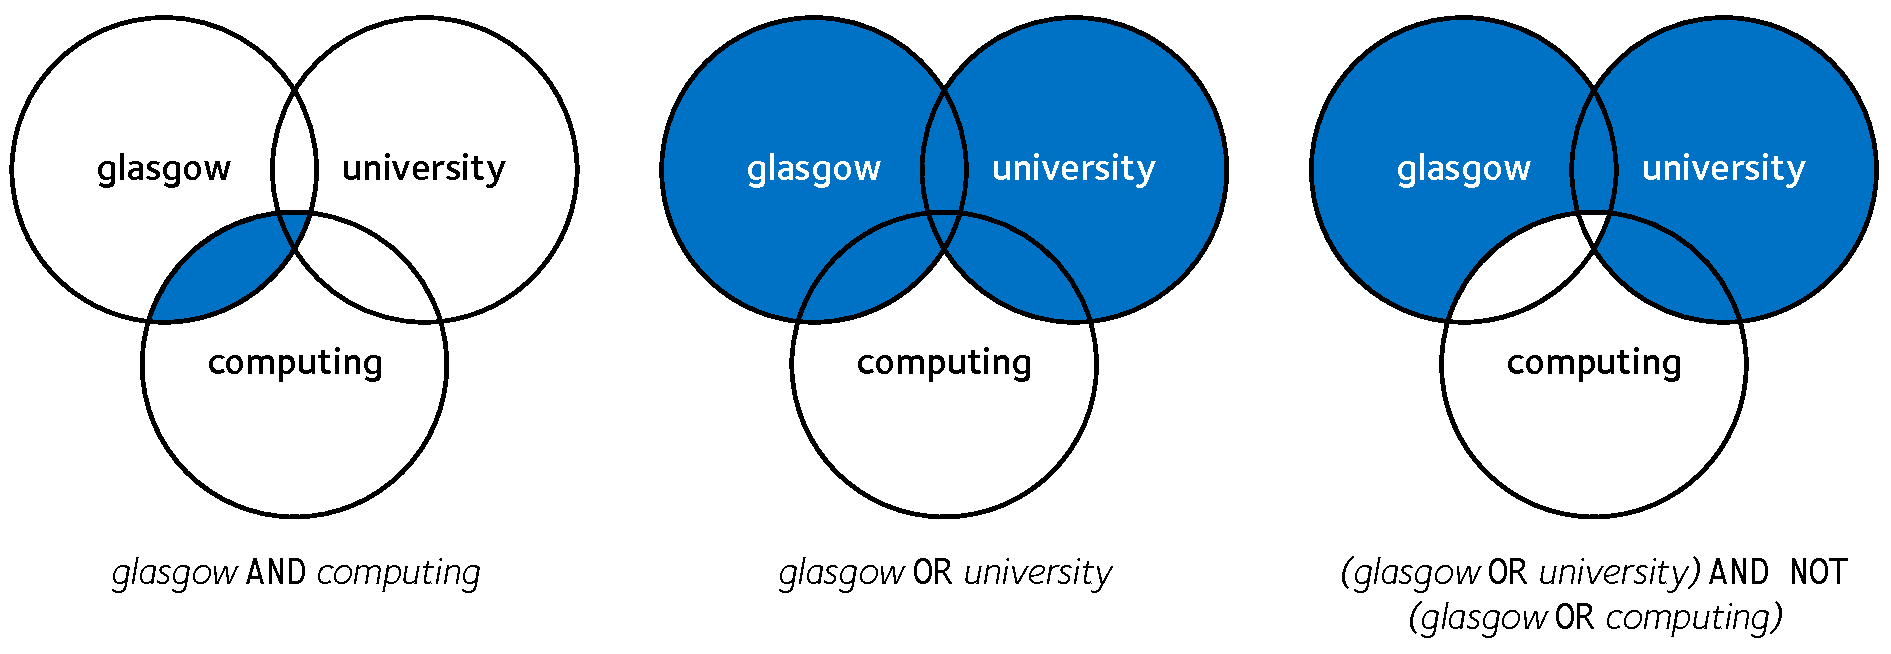
\includegraphics{figures/ch2-boolean.pdf}}
    \caption[Venn diagrams illustrating boolean retrieval]{An example illustration of the boolean retrieval model, using the query terms \texttt{glasgow}, \texttt{university} and \texttt{computing}. Each disc represents the set of documents containing that particular term. In the figure, three Venn diagram examples are provided, demonstrating the key logical operators used (\texttt{AND}, \texttt{OR} and \texttt{NOT}). Areas in blue are returned in the example boolean query provided underneath each Venn diagram.}
    \label{fig:boolean}
\end{figure}

By considering an individual query term as an unambiguous set of documents, logical operations can be applied to retrieve a set of documents. For example, the query term \texttt{glasgow} will yield a set of all documents containing the term \texttt{glasgow}, yet the query \texttt{NOT glasgow} will retrieve the set of documents that \emph{does not} contain any mention of the term \texttt{glasgow}. The results of applying logical operators between different sets can be illustrated through a Venn diagram, where each set of documents is represented as a disc. Figure~\ref{fig:boolean} provides an example of such diagrams.

Despite the relative simplicity of this approach, there are major limitations. First, when considering the query, there is no notion of term importance -- every term has equal weighting. Queries utilising logic rules also appear to be relatively unnatural representations of an information need. Indeed, as the information need become more complex, the boolean query can grow to be disproportionally large and cumbersome to interpret (refer to the right Venn diagram of Figure~\ref{fig:boolean}). This would be especially true when a complex information need is represented as a boolean query. As documents either belong to a set or they don't, a document is either useful (\texttt{TRUE}) or not (\texttt{FALSE}). As such, one cannot estimate a degree to how relevant a document would be to the searcher's query, and thus results are provided to the searcher unranked.

Returning an unranked set of documents would appear as an alien concept to users of~\gls{acr:ir} systems today -- one would assume that the document presented first would be the document considered most likely to be useful as per the underlying retrieval model. This would make it difficult for a searcher to obtain some notion of how many results he or she should examine before stopping, as all terms and documents are considered equal. Despite not being required in contemporary~\gls{acr:ir} systems, many do still provide support for crafting a boolean query for when returning a good set of results is difficult. This may for example be useful when there is ambiguity in the searcher's information need, and clarification is required to eliminate a set of unhelpful documents. Boolean queries also find traction in patent searching, where \emph{recall} rather than \emph{precision} is preferred (refer to Section~\ref{sec:ir_background:evaluation}).

\subsubsection{Vector Space Model}
With major weaknesses present in the boolean retrieval model, work then progressed to develop more advanced approaches that mitigated the issues raised above.~\cite{luhn1957ranking_query} hypothesised that a searcher, when wishing to search for documents addressing their information need, should prepare a document that is similar to the documents that were sought after. By comparing documents against this \emph{representative} document, a system could begin to deduce what other documents would be useful, and by what margin.

The vector space model proposed by~\cite{salton1975vsm} incorporates the principles as outlined by~\cite{luhn1957ranking_query}. These basic principles are operationalised by representing queries and documents within Euclidean geometry, where both are represented as vectors in multi-dimensional space. The notion of how close documents appear to each other denotes the usefulness of a document.

The vector space model is popular, as it provides an intuitive means for addressing the overarching problem of an~\gls{acr:ir} system, and can incorporate methods such as term weighting which have been shown to improve retrieval effectiveness~\citep{croft2010search}. Furthermore, as queries and terms are represented in Euclidean space, vector similarity methods can be employed to determine relevance/usefulness. While many approaches have been trialled, empirical evidence has favoured \emph{cosine similarity}~\citep{croft2010search}. This is aptly illustrated in Figure~\ref{fig:vector_space}. Using such an approach allows one to then compute the degrees of relevance/usefulness, meaning that matched documents can be returned in a ranked order. This ranking than then be potentially utilised by a searcher to determine a cutoff point at which he or she should stop examining results.

\begin{wrapfigure}[13]{r}{0.45\textwidth}
    \begin{center}
    \vspace*{-10mm}
    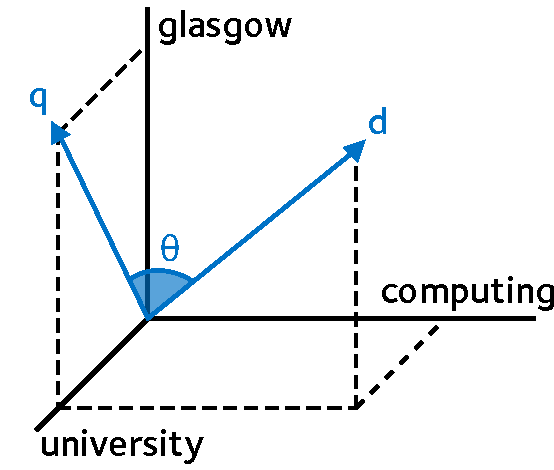
\includegraphics[width=1\textwidth]{figures/ch2-vector.pdf}
    \end{center}
    \vspace*{-4mm}
    \caption[Vector Space Model (Cosine similarity)]{An illustration of the Vector Space Model in Euclidean space, with each term representing a dimension. Here, the cosine similarity between query \emph{q} and document \emph{d} is shown.}
    \label{fig:vector_space}
\end{wrapfigure}

In order to understand the basic workings of the vector space approach, let us consider a query, $Q$, with each of its constituent terms placed within a term vector in $t$-dimensional space, leading to $Q = (q_1, q_2, q_3,\dotsc, q_{it})$. Consider also a document, $D_i$, with terms from the document again represented in $t$-dimensional space, yielding $D_i = (d_{i1}, d_{i2}, d_{i3},\dotsc, d_{it})$. From this notation, $d_{ij}$ represents the \emph{term frequency (TF)} of term $j$ appearing in document $i$. With each term represented as a separate dimension within Euclidean space, a weighting scheme can be subsequently applied to emphasise or understate more discriminative or less discriminative terms, respectively. An example of less discriminative terms would for example be stopwords, as described in Section~\ref{sec:ir_background:basics:indexing:stopwords}. By applying weighting schemes, the vector space model at a stroke overcomes a previously discussed limitation of the boolean model in that all terms are weighted equally.

Term frequency is one of many different term weighting schemes that have been trialled over the years in~\gls{acr:ir} research. Perhaps one of the best and widely used schemes is \emph{inverse document frequency (IDF)}, proposed by~\cite{sparck1972statistical}. Here, the frequency of a term is normalised against the length of a given document. In the words of its creator, IDF allows for one to define the specificity of a term as \emph{``an inverse function of the number of documents in which it occurs.''}~\citep{sparck1972statistical}. This is useful as non-discriminative terms that occur frequently within an index (e.g. \texttt{the}) would have its weight diminished, with the inverse happening for more discriminative terms, better able to describe a given document.

TF and IDF are typically combined together as a measure of both term appearance and importance, under an approach called \emph{TF-IDF}. For a given term $k$, one can calculate a TF-IDF score with the following equation: $ 2 3 4 $

\begin{equation*}
tf_{i,k} \cdot idf_{k} = \frac{f_{i,k}}{\sum_{j=1}^{t} f_{i,j}} \cdot log \frac{N}{n_k}.
\end{equation*}

Above, $f_{i,k}$ is the frequency of term $k$, $N$ is the number of documents in the collection used, and $n_k$ is the number of documents in which term $k$ appears at least once.

\subsubsection{Probabilistic Models}
From boolean to vector space retrieval models, a further model emerged based upon \emph{probability theory}. Probability theory allows one to define a means to formally model the relevance and/or usefulness of a document to a searcher's query, given \emph{uncertainty} about their precise information need. One of the most widely referred to ranking principles, known as the \emph{Probability Ranking Principle (PRP)} (defined by~\cite{robertson1977prp} -- who in turn attributed the development to~\cite{cooper1971relevance}), states the following.

\begin{quote}
\emph{``If a reference retrieval system's response to each request is ranking of the documents in the collections in order of decreasing probability of usefulness to the user who submitted the request, where the probabilities are estimated as accurately as possible on the basis of whatever data has been made available to the system for this purpose, then the overall effectiveness of the system to its users will be the best that is obtainable on the basis of that data.''}
\attrib{\cite{robertson1977prp}}
\end{quote}

Essentially, this states that documents that are considered more likely to be relevant than non-relevant should be retrieved -- or where $P(R|D) < P(\overline{R}|D)$. However, while the PRP lays much of the foundation from which probabilistic retrieval models have been derived, it does not itself provide a concrete implementation of such a model. The framework provided by the PRP in order to score a document to a searcher's query is:

\begin{equation*}
score(d,q) = P(rel|q,d) \approx \sum_{t \in q}wt_{t,d}.
\end{equation*}

Above, $rel$ is defined as the relevance probability of document $d$, given query $q$. Early approaches following this framework utilised Bayes' theorem to define the probability of a document being relevant to the associated query, based upon the likelihood of drawing query terms from relevant and non-relevant documents. This was considered as a classification problem, where documents were considered as either relevant or non-relevant to said query. The aforementioned likelihood has been computed by many models -- perhaps the most important being \emph{Okapi BM25}~\citep{robertson1995trec3}. Indeed, this retrieval model has had considerable impact upon the~\gls{acr:ir} community and is still used extensively today, providing a solid baseline for contemporary research. This model is employed as the basic retrieval model for experimentation in this thesis due to its effectiveness and popularity.

\subsubsection{Language Models}\label{sec:ir_background:basics:models:language}
The final retrieval model family that we discuss are language models, closely related to the probabilistic model we define above. Indeed, while such probabilistic models have been demonstrated to perform well empirically, adapting the PRP and subsequent developments to more advanced approaches has been difficult and is generally not intuitive~\citep{hiemstra2000language_modelling} -- the interpretation offered by probabilistic models may be considered loose, and is not always theoretically principled~\citep{whiting2015phd}. This has led to the development of more formalised statistical language modelling approaches, as defined in the fields of \emph{Natural Language Processing (NLP)}, for example~\citep{lavrenko2001language_models}.

Given the strong rooting in the principles of language and associated fields, language models provide a solution to the so-called \emph{bag of words}~\citep{harris1954distributional} concept that a majority of preceding retrieval models subscribe to. Put simply, this concept considers each document and query as a bag of words, meaning that the ordering of terms loses any significance. While a simplifying assumption, losing the ordering of terms means that semantic meaning and grammar rules are lost -- and thus a retrieval engine employing a model using this simplifying assumption may lose key meanings, and subsequently retrieval effectiveness will suffer.

Essentially, a language model is a probability distribution over strings of text. Given a string of text (i.e. a searcher's query), how likely is it that the given query appears in a given \emph{language}? Each document provides its own language, where we consider all possible phrases that the author of a document could have written when creating said document. Of course, some phrases are more likely than others. For example, the phrase \texttt{rain in glasgow} is more likely to appear in a document (in that order) than the seemingly random assortment of terms \texttt{purple monkey dishwasher}\footnote{If you ever watched \emph{The Simpsons}, you might disagree with this statement.}. Given this, and conceptualising a searcher's query in much the same fashion, we can produce a probability distribution $P(Q|D)$, concerning the probability of observing query $Q$ during some form of sampling within the language model of document $D$.

The most simplistic approach to language modelling is undoubtedly the \emph{unigram} approach, where each term within a document and/or query are considered in isolation, which subscribes to the aforementioned simplifying bag of words concept. Essentially, such an approach provides a probability distribution over the words appearing in the language. Higher order \emph{grams} such as \emph{bi-grams} and \emph{tri-grams} begin to consider more the place in which terms appear with respect to others, and thus the semantic meaning defined by this positioning begins to be taken into account within the probability distribution. When considering a document, the more a document discusses a particular topic, the more likely one would begin to observe terms about that topic in said document. When a term is not mentioned in a document, smoothing can be applied (given the wider collection the document is part of) to avoid a zero probability when calculating the probability of terms permitting the partial matching of queries where not all terms appear within a target document.

\subsection{System-Based Evaluation}\label{sec:ir_background:evaluation}
Given the \emph{de facto} architecture of an experimental~\gls{acr:ir} system (Section~\ref{sec:ir_background:basics:cranfield}) and the numerous retrieval models that one can employ (Section~\ref{sec:ir_background:basics:models}), how can we then begin to evaluate a given retrieval system? Recalling that the \emph{modus operandi} of such a system is to satisfy the needs of the searchers who utilise it,~\cite{lancaster1968information} provides three criteria by which an~\gls{acr:ir} system can be evaluated:

\begin{itemize}
    \item[\emph{(i)}]{the suitability of an~\gls{acr:ir} system in terms of the specific tasks for which it will be used;}
    \item[\emph{(ii)}]{the~\gls{acr:ir} system's task performance \emph{efficiency}; and}
    \item[\emph{(iii)}]{the extent to which the system satisfies the information needs of its \emph{users.}}
\end{itemize}

These three criteria can themselves be subsequently split into two separate categories: approaches that consider how well the \emph{system} performs (i.e. criterion \emph{(i)} and \emph{(ii)}); and with regards to the individual who is using the~\gls{acr:ir} system at the time (\emph{user-orientated}, criterion \emph{(iii)})~\citep{voorhees2005trec_book}. Given the title of this section, we subsequently only consider system-orientated evaluation approaches here; a more detailed explanation of a user's role and how we can evaluate their performance is provided in Section~\ref{sec:ir_background:user:evaluation}.

Considering system-orientated measures of evaluation, one can consider a system's \emph{efficiency} or \emph{effectiveness}. Efficiency concerns some form of operational metric, such as the speed of the~\gls{acr:ir} system. This example is important (especially in commercial web search engines) as even a fractional increase of the time taken to return results to a searcher can reduce the number of returning searchers, and impacts search engine revenue~\citep{brutlag2009speed}.

However, when one thinks of~\gls{acr:ir} evaluation, they usually think about how \emph{effective} the system is. Of course, the definition of what defines an~\gls{acr:ir} system to be effective hugely depends upon the type of search task being undertaken. A patent searcher would for example expect an~\gls{acr:ir} system to return \emph{all} relevant patents to avoid missing a related patent (and thus incurring penalties) -- whereas a casual web searcher curious about a topic they know little about (i.e. ad-hoc) would be satisfied with a single, relevant result.

As such, this section provides a brief overview of the basic effectiveness measures widely used within~\gls{acr:ir} today. We consider four different measures. It should be noted that such measures are usually computed from \emph{batch-style} experimentation with up to $1,000$ results available to obtain the best approximation possible.

\blueboxheader{Other Evaluation Measures}
We acknowledge that the measures discussed in this section are only a subset of the wider, full range of measures that have been developed and trialled in~\gls{acr:ir} research. Examples include the \emph{F-Measure,} the harmonic mean between precision and recall. Measures that we discuss are those that we report in the empirical work of this thesis.

\begin{figure}[t!]
    \centering
    \resizebox{1\hsize}{!}{
    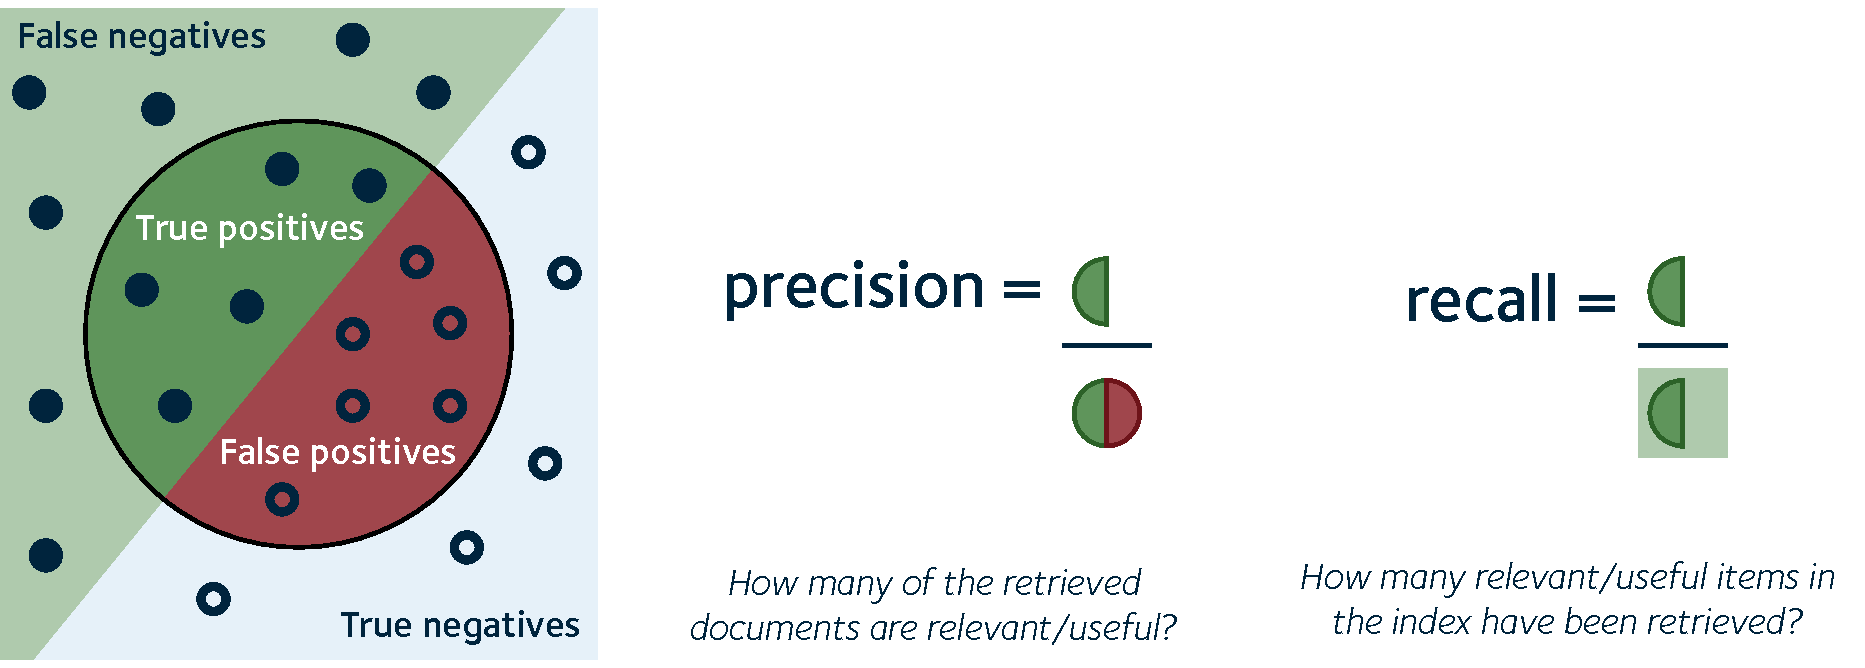
\includegraphics{figures/ch2-pr.pdf}}
    \caption[Precision and recall]{An illustration of precision and recall. On the left is an illustrated example of an index, containing many documents. The large circle represents the set of documents retrieved for a query. Documents that are relevant to the query are represented as~
\includegraphics[height=\fontcharht\font`\d]{figures/ch2-pr-r.pdf}, with non-relevant documents represented as~
\includegraphics[height=\fontcharht\font`\d]{figures/ch2-pr-nr.pdf}. Note that not all relevant documents are retrieved; doing so would mean that the retrieval engine used would have produced perfect results. From the illustration on the left, definitions of \emph{precision} and \emph{recall} are also provided.}
    \label{fig:pr}
\end{figure}

\subsubsection{Precision}\label{sec:ir_background:evaluation:precision}
The \emph{precision} ($P$) of an~\gls{acr:ir} system considers the fraction of documents that have been retrieved that are considered to be relevant or useful to the searcher's given query, information need. An~\gls{acr:ir} system that yields high precision is regarded as one that performs well.

Figure~\ref{fig:pr} provides a visual illustration of what precision entails (as well as its counterpart, \emph{recall}, which is discussed below). Given the set of all documents within an index, an~\gls{acr:ir} system will retrieve a number of these documents that satisfy the criteria set out in the retrieval model employed. Of the documents retrieved, some will be considered relevant to the searcher's information need; others will be considered non-relevant. As such, prior knowledge of the relevance of particular documents to given topics is therefore required (e.g. TREC QRELs, as defined in Section~\ref{sec:ir_background:basics:cranfield:trec}).

Precision can therefore be defined as:

\begin{equation*}
precision = \frac{|~\text{\emph{relevant documents}}~\cap~\text{\emph{retrieved documents}}~|}{|~\text{\emph{retrieved documents}}~|}.
\end{equation*}

Research in~\gls{acr:ir} typically reports precision up to a particular rank, i.e. $P@k$. For example, $P@10$ will provide a fractional value for the number of relevant documents that appeared within the top $10$ results of a query. Herein lies one of the most elementary and basic \emph{stopping models} that we find encoded within various measures and models defined by~\gls{acr:ir} researchers over the years -- stopping at $10$\footnote{The value of $k=10$ is often chosen in~\gls{acr:ir} research as it has been shown that this is typically the depth to which searchers would look through web search results~\citep{jansen2006www}.}, or $k$, denotes that a system or searcher need not bother examining any further documents.

\subsubsection{Recall}
While precision considers the fraction of documents retrieved that are relevant, \emph{recall} ($R$) considers the fraction of documents that were retrieved and relevant to a query against \emph{all known relevant documents for a query}. Recall can formally be defined as:

\begin{equation*}
recall = \frac{|~\text{\emph{relevant documents retrieved}}~|}{|~\text{\emph{relevant documents}}~|}
\end{equation*}

Considering the patent searching example defined above, high recall would be desirable in this type of task -- high recall means more patents matching the searcher's query will be returned, thus reducing the possibility of missing important prior filings.

Given more modern retrieval models, the notion of ranking would lead a searcher to assume (as per the PRP~\citep{robertson1977prp}) that relevant documents pertaining to their query will be the first results presented. Non-relevant documents will also of course appear, typically leading to some form of tradeoff between precision and recall, as discussed below. The tradeoff considers the notion that as you increase recall, the number of non-relevant items will undoubtedly also increase, thus reducing the~\gls{acr:ir} system's overall precision.

% \subsubsection{F-Measure}
% Considering the aforementioned tradeoff between precision and recall, the \emph{F-measure}, which represents a \emph{weighted, harmonic mean} between the two. Originally proposed by~\cite{rijsbergen1979ir}, the measure was provided to \emph{``measure the effectiveness of retrieval with respect to a user who attaches $\beta$ times as much importance to recall as precision.''} The F-measure, along with its $\beta$ parameter, is defined by~\cite{chinchor1992f_measure} as:
%
% \begin{equation*}
% F_\beta = \frac{(\beta^2 + 1)\cdot PR}{\beta^2 \cdot P + R}\hspace{10mm}(0\leqslant\beta\leqslant+\infty).
% \end{equation*}
%
% Above, $P$ and $R$ denote precision and recall respectively. $\beta$ is simply used as a parameter for controlling the balance between the two. When $\beta = 1$, $F_1$ is equivalent to the harmonic mean of precision and recall. Since the terms F-Measure and harmonic mean are ubiquitously linked (somewhat \emph{harmoniously}\dots), the two terms are used interchangeably within the literature. As $\beta$ tends towards $0$, the score becomes more precision orientated.

\begin{figure}[t!]
    \centering
    \resizebox{1\hsize}{!}{
    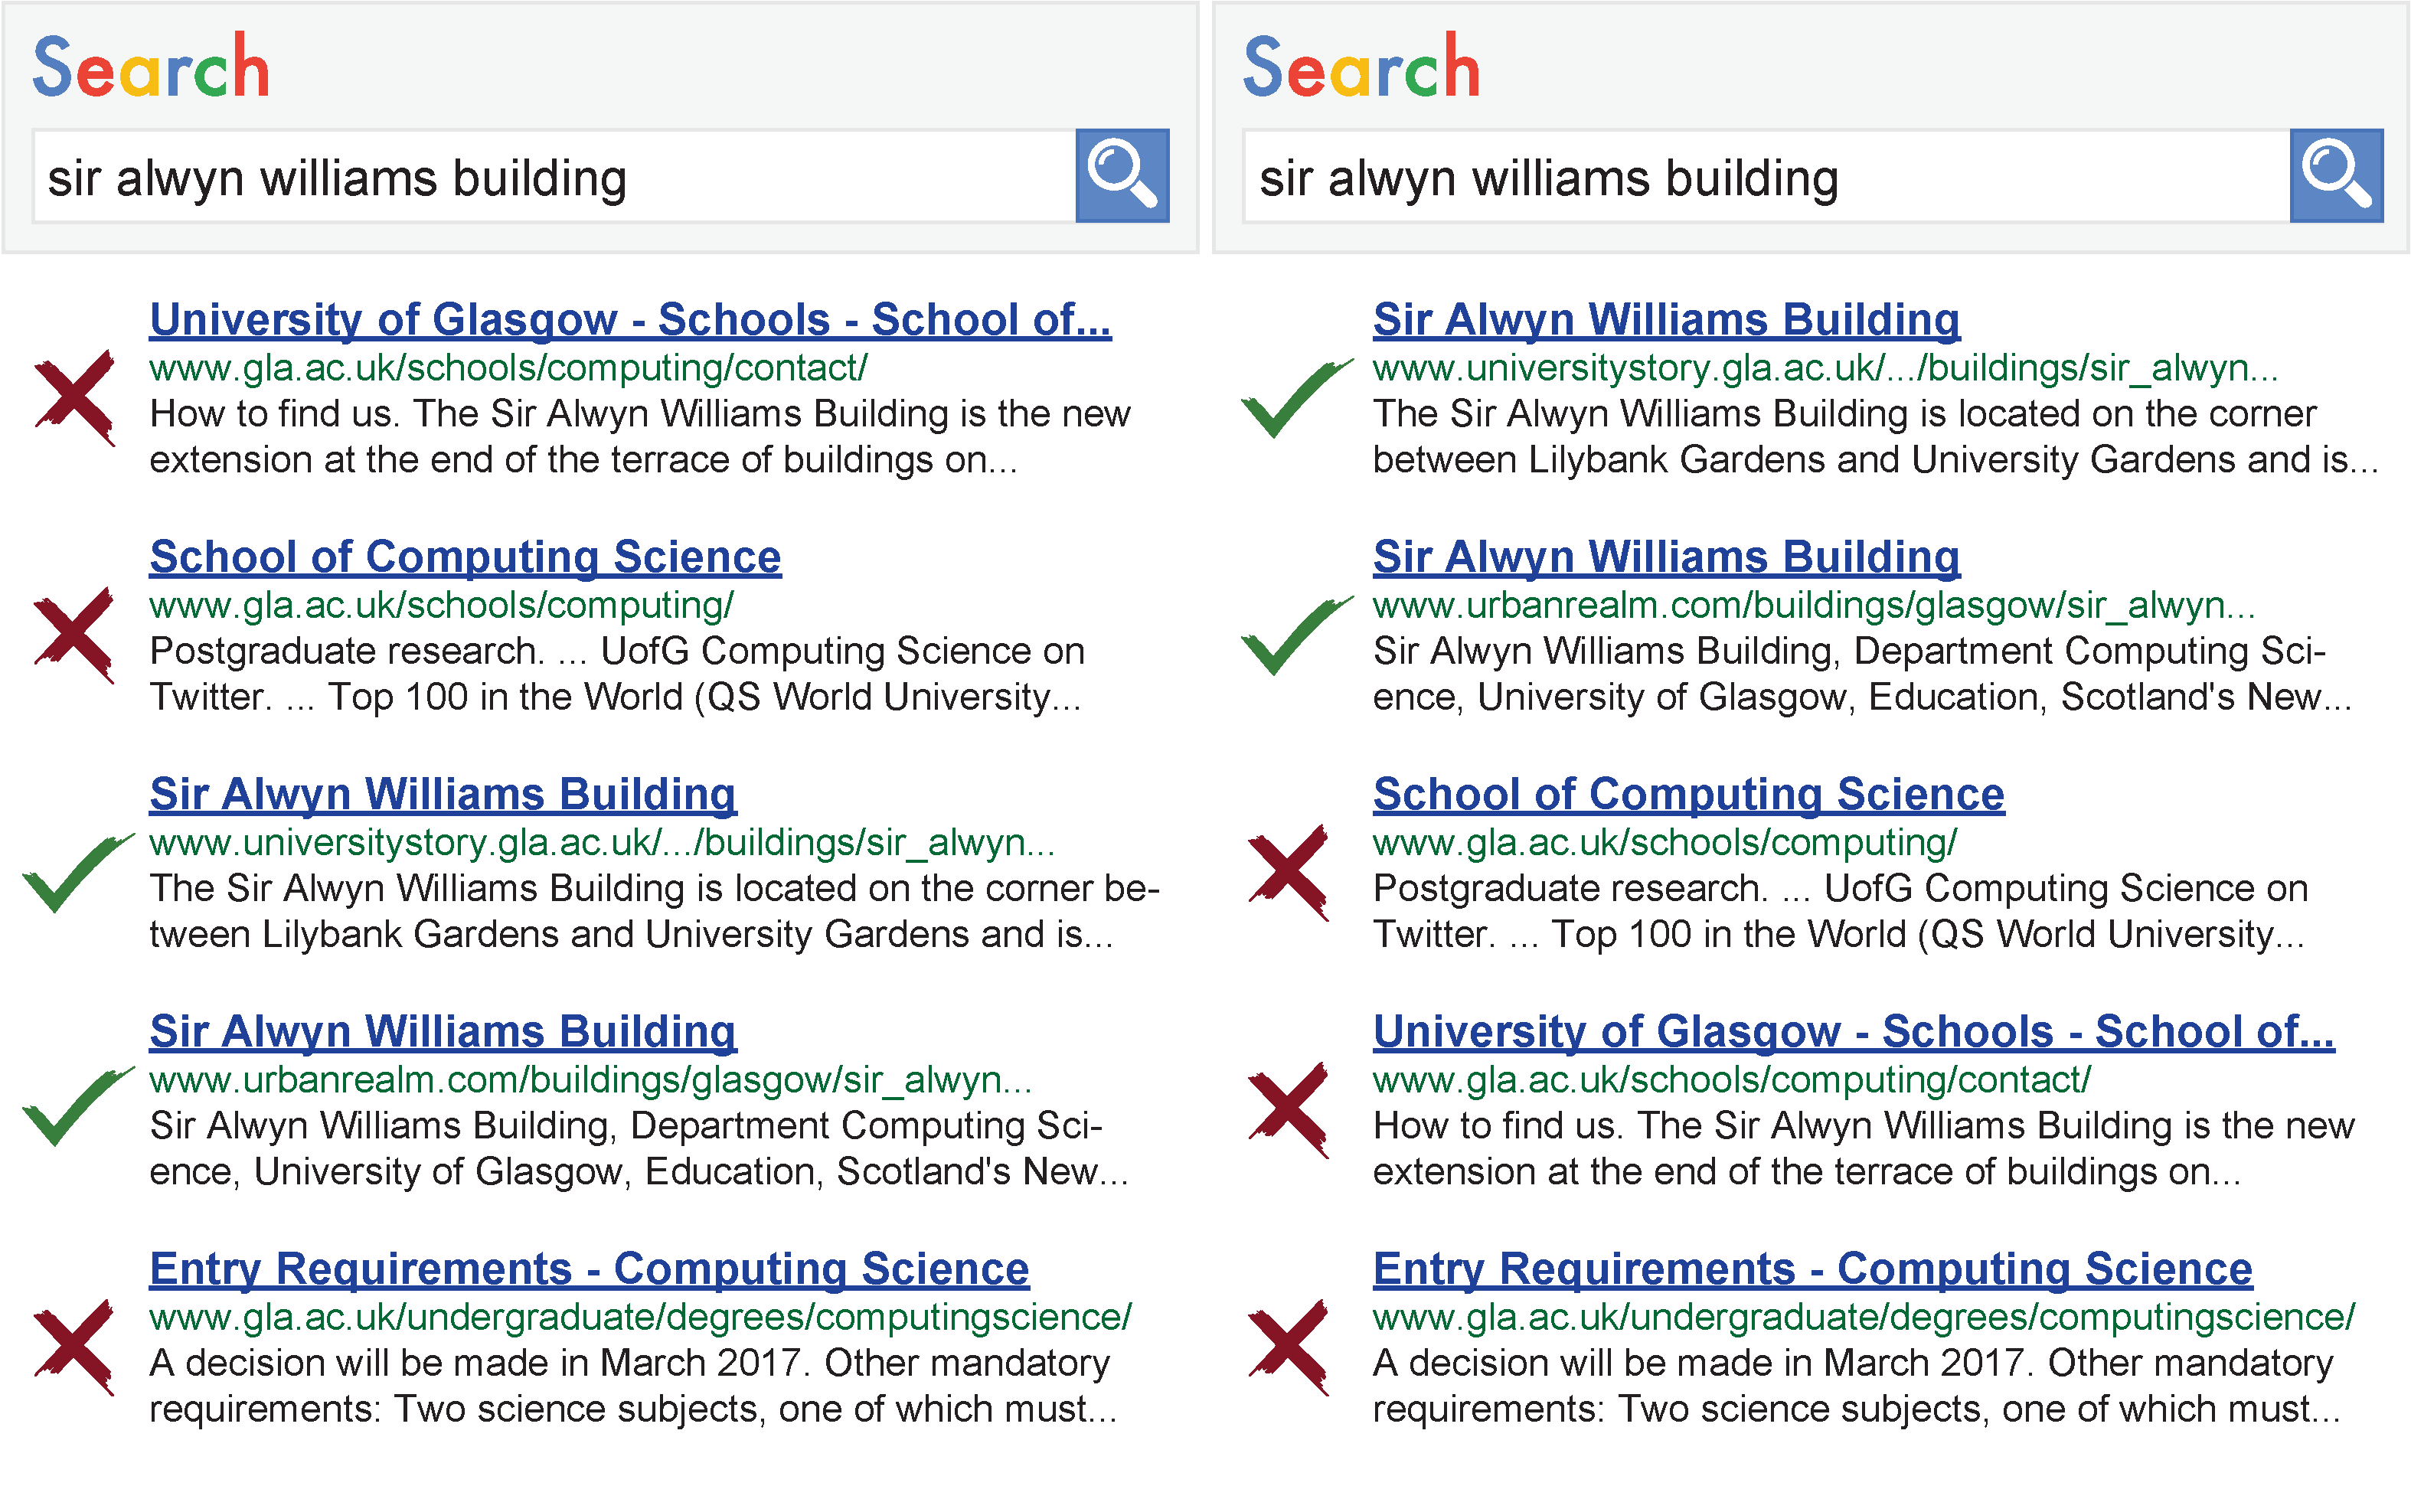
\includegraphics{figures/ch2-ranking.pdf}}
    \caption[The importance of ranking]{Given an information need to find out information about the \emph{Sir Alwyn Williams Building} (part of the University of Glasgow's estate portfolio), which ranked list of results would you prefer to make use of?}
    \label{fig:ranking}
\end{figure}

\subsubsection{Mean Average Precision}
One of the major limitations of the previously examined measures is that the \emph{ranking} of results is not specifically taken into consideration. For example, consider Figure~\ref{fig:ranking}. Looking at the {\color{dmax_green}ticks} and {\color{dmax_red}crosses} (denoting relevant and non-relevant content, respectively) within the figure, would it be desirable to be presented with the list of results ranked in order shown on the left, or on the right? Despite apparent differences in the ranking of results, precision for example would show no difference -- both ranked lists contain two relevant documents, and three non-relevant. A simple calculation would show that the $P@5$ score for both lists would therefore be $2 / 5 = 0.4$ -- there is no discernible difference between them.

One of the most widely used measures that addresses this issue -- and provides a means of quantifying the all-round effectiveness of a retrieval system for a representative set of test topics -- is \emph{Mean Average Precision (MAP)}~\cite{voorhees2005trec_book}. Rather than considering a single set of results, MAP can consider multiple queries -- and, as alluded to above, considers the ranking in which results for each query are provided.

As the name might imply, MAP provides a mean over the \emph{Average Precision (AP)} for each topic that is examined. AP provides the rank sensitive component of MAP up to some cutoff $k$, as defined below:

\begin{equation*}
AP = \frac{\sum^{n}_{k=1}(P(k) \cdot rel(k))}{|~\text{\emph{relevant documents}}~|}.
\end{equation*}

Above, $P(K)$ is the precision cutoff at rank $k$ (i.e. $P@k$), and $rel(k)$ is a function to denote the relevance of a particular document at rank $k$. This is assumed to be binary, with $1$ denoting a relevant document, and $0$ denoting a non-relevant document. AP is then computed for each sample query, $q$, over the set of topics $T$ to produce a final MAP score for the~\gls{acr:ir} system:

\begin{equation*}
MAP = \frac{\sum^{T}_{q=1} AP(q)}{|~Q~|}.
\end{equation*}

\subsubsection{Expected Search Length}\label{sec:ir_background:evaluation:esl}
Given a series of well established measures, we now consider the so-called \emph{Expected Search Length (ESL)}~\citep{cooper1968expected_search_length} of a searcher. Put simply, the expected search length is the number of non-relevant documents that a searcher will have to search through to obtain a \emph{desired number of relevant documents.} Therefore, systems demonstrating a shorter expected search length are considered to be more effective than systems with a comparatively longer expected search length. In other words, the measure indicates how much wasted search effort one would expect using a given retrieval system, as opposed to randomly searching until the needed relevant documents are found.

From~\cite{cooper1968expected_search_length}, the expected search length can be computed thus:

\begin{equation*}
ESL(q) = j + \frac{i \cdot s}{r + 1}
\end{equation*}

\noindent
where $q$ represents some query, and $j$ represents the number of non-relevant documents when considered to query $q$. This is the minimum number of documents that must be found in order to satisfy the searcher's information need -- this is the minimum number before $s$ of the $r$ total relevant documents are found by the searcher.

\section{Considering the User}\label{sec:ir_background:user}
So far in this chapter, we have provided a background on several key developments in the area of~\gls{acr:ir} research. However, these aforementioned developments all purely consider the \emph{system} that is being evaluated (i.e \emph{system-sided} research). To reiterate once more, the overall goal of an~\gls{acr:ir} system is to satisfy some information need that a searcher, or \emph{user}, acquires. In short, satisfying the user is key to~\gls{acr:ir}. Central to this is our understanding and incorporation of a user's search behaviours and interactions into the evaluation of~\gls{acr:ir} systems~\citep{callan2007minds}.

The study of~\glsfirst{acr:iir} attempts to address this gap in our collective knowledge.~\gls{acr:iir} studies can include aspects from user-sided and system-sided research. For example, one might present results of a user study examining a particular phenomenon of a user's behaviour, and also provided details of a system-sided evaluation. As discussed by~\cite{kelly2009iir},~\gls{acr:iir} can trace its roots back to a variety of different disciplines, including: traditional~\gls{acr:ir}; library and information science; psychology; and~\gls{acr:hci}. Typically presented as branch of~\gls{acr:ir} and/or~\gls{acr:hci}, arguments also exist to consider~\gls{acr:iir} as a distinct area of research~\citep{ruthven2008iir}.

\begin{quote}
\emph{``In~\gls{acr:iir}, users are typically studied along with their interactions with systems and information. While classic~\gls{acr:ir} studies abstract humans out of the evaluation model,~\gls{acr:iir} focuses on users' behaviors [sic] and experiences -- including physical, cognitive and affective -- and the interactions that occur between users and systems, and users and information. In simple terms, classic~\gls{acr:ir} evaluation asks the question, does this system retrieve relevant documents?~\gls{acr:iir} evaluation asks the question, can people use this system to retrieve relevant documents?''}
\attrib{\cite{kelly2009iir}}
\end{quote}

In order to aptly describe where~\gls{acr:iir} fits into the system-sided vs. user-sided space,~\cite{kelly2009iir} also provided an intuitive spectrum of work in this area, comprised of eight types of study -- as shown in Figure~\ref{fig:spectrum}. Below, we provide a brief explanation of the key types of study as shown in the spectrum.

\begin{figure}[t!]
    \centering
    \resizebox{1\hsize}{!}{
    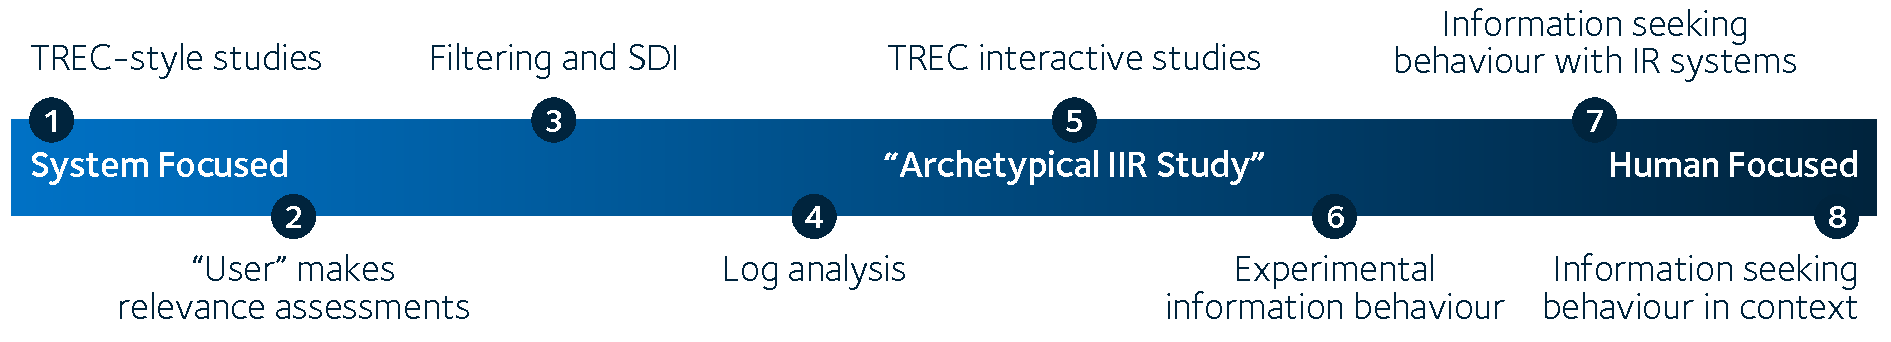
\includegraphics{figures/ch2-spectrum.pdf}}
    \caption[Spectrum IIR research~\citep{kelly2009iir}]{The spectrum of conceptualising IIR research. Methods on the left consider a more system-focused approach, with those on the right considering a more user-focused approach. The fifth step within the spectrum considering TREC interactive studies is considered to be an \emph{"archetypical~\gls{acr:iir} study"}. Figure adapted, with permission, from~\cite{kelly2009iir}.}
    \label{fig:spectrum}
\end{figure}

\begin{itemize}
    
    \item[\emph{(1)}]{\blueboxbold{TREC-style studies} focus on the development and evaluation of system-sided research, such as retrieval models and indexing methods. These would be considered akin to most of the studies undertaken in TREC tracks over the years (excluding tracks such as the Interactive Track, for example). No real users are utilised using this approach, although we do argue that there is a simplistic \todo{\emph{user model}} encoded within this approach. Human assessors however create judgements used for evaluation, but they do not function as searchers as such. Assessors are the only humans \emph{in the loop} for this type of study -- the rest is fully automated on computers.}
    
    \item[\emph{(2)}]{\blueboxbold{'User' relevance assessment studies} do consider humans \emph{in the loop}, but this time for exceptionally limited purposes. As the name for these studies may suggest, humans are employed for generating relevance assessments as part of the study, and as such, no searching takes place.~\cite{bota2016information_cards} undertook a study of this nature, where they examined search behaviour for predefined queries when presented with a series of \emph{information cards}\footnote{An \emph{information card} is a contemporary feature of a~\gls{acr:serp}, typically presented on the right rail of the page. They provide additional information to the topic in question, such as images and basic statistics of the entity.}}.
    
    \item[\emph{(5)}]{Moving along the spectrum,~\cite{kelly2009iir} cites~\blueboxbold{TREC interactive studies} in which typically a system and/or interface feature is evaluated. Typically, the feature is related to the human, such as examining their behaviour, cognition or information seeking context. These studies usually aim to assist in aiding our understanding of the search process, and to aid in the development of more intuitive and user-friendly search interfaces.}
    
\end{itemize}

The studies complying with point \emph{(5)}, called \emph{archetypical~\gls{acr:iir} studies}~\citep{kelly2009iir}, are the studies which we largely consider in this thesis -- indeed, later on in this thesis, we consider a variety of aspects that can influence the behaviour and performance of searchers. Moving further along the spectrum, the study of users becomes ever more prominent, until we reach:

\begin{itemize}
    
    \item[\emph{(8)}]{\blueboxbold{information seeking behaviour in context studies} which considers research that (almost) exclusively focuses on users. Here, we consider the information needs of the individuals~\gls{acr:ir} systems aim to satisfy -- searchers. Researchers typically would examine a user search, while collating qualitative data about their experiences.}
    
\end{itemize}

Of course, a more detailed explanation of these different types of study can be found in the work by~\cite{kelly2009iir} that illustrate the more user-centric approaches in detail. We now however turn our attention back to the idea of employing simulation and a form of \emph{user model} in order to better understand a searcher's complex interactions during the search process.

\subsection{Considering User Models}\label{sec:ir_background:user:models}
Models of the search process attempt to capture the high level, cognitive processes that a searcher undertakes during a search session -- such as issuing a query, or examining a document for relevance. User models of the search process have been present in more system sided~\gls{acr:ir} research for a number of decades (as discussed in Section~\ref{sec:ir_background:user}), as well as implicitly encoded within the variety of measures that have been used.

\cite{carterette2011models} argues that the measures widely used within the~\gls{acr:ir} community are themselves typically comprised of three, distinct underlying models:

\begin{enumerate}
    \item{a \emph{browsing model}, describing how a searcher interacts with a search engine and the subsequent~\glsplural{acr:serp} that are presented to them;}
    \item{a model encoding some form of \emph{document utility} that provides a description for how utility can be derived from relevant documents; and}
    \item{a \emph{utility accumulation model} that describes how a searcher accumulates utility over the course of a search session.}
\end{enumerate}

Of particular interest to the work in this thesis are the \emph{browsing models} that attempt to capture the broad interactions that take place between the searcher and the search engine. One of the most well developed browsing models highlighted by~\cite{carterette2011models} is that of a searcher, after issuing a query, examines a series of documents presented to him or her on the resultant~\gls{acr:serp} one by one (in a linear fashion), and at some depth, $k$, stops. This is the basic model followed by measures such as $P@k$, for example. (refer to Section~\ref{sec:ir_background:evaluation:precision}). This process is illustrated with a flowchart in Figure~\ref{fig:basic_model}.

\begin{figure}[t!]
    \centering
    \resizebox{1\hsize}{!}{
    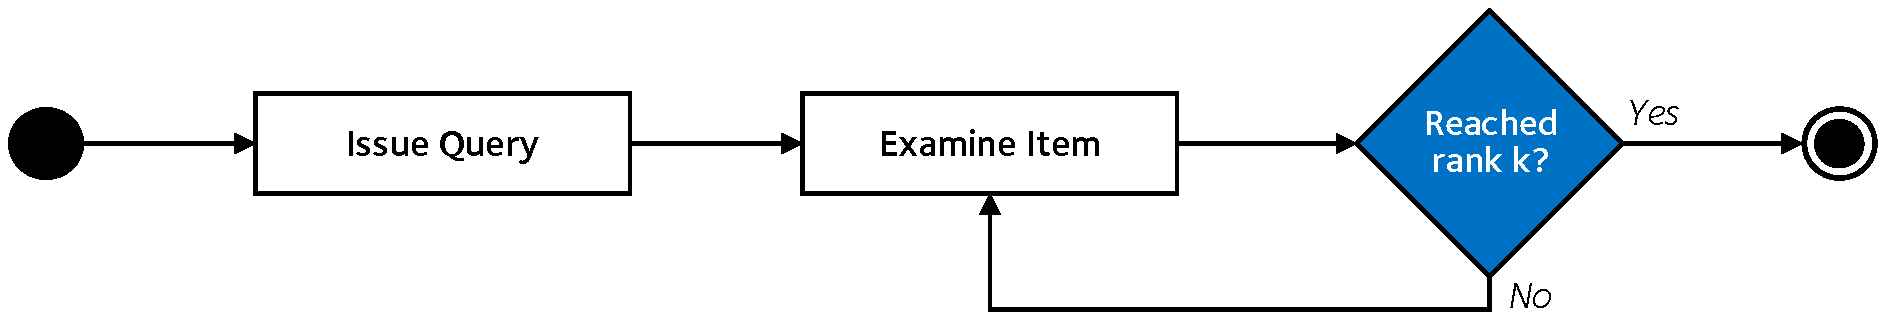
\includegraphics{figures/ch2-basic_model.pdf}}
    \caption[A basic user model of search]{A basic model of the search process. Here, a searcher, after issuing a query to the underlying search engine, examines a number of different items presented to him or her before deciding to stop at some rank \emph{k}. This basic approach is widely used in many measures of~\gls{acr:ir} effectiveness, and is considered by~\cite{carterette2011models} as a form of \emph{browsing model}, capturing the interactions that take place between the searcher and search engine.}
    \label{fig:basic_model}
\end{figure}

While perhaps deficient in terms of representing a real-world searcher's behaviours, this basic model has served the~\gls{acr:ir} community well for a number of decades, and works well in batch-style experimentation that is common in the community. While more advanced models of the search process have been developed, we leave these to Section~\ref{sec:stopping_background:models:conceptual}. Instead, we now consider the notion that with a user model of the search process, we can then take this model to provide a \emph{simulation} of the interactions that take place.

\subsection{Simulation in~\gls{acr:ir} and~\gls{acr:iir}}\label{sec:ir_background:user:simulation}
As outlined in Section~\ref{sec:intro:simulation}, simulation provides a powerful tool for conducing low-cost, reproducible research~\citep{azzopardi2010workshop}. As discussed by~\cite{fishwick1995simulation}, simulation allows one to solve a large variety of systems, without the need to resort to a \emph{``bag of tricks'',} whereby one must choose special purpose and sometimes arcane solutions.

Simulation has of course been extensively used within~\gls{acr:ir} and~\gls{acr:iir}. As discussed by~\cite{gordon1990evaluating}, much of the classical work in~\gls{acr:ir} employing simulation addressed issues such of \emph{retrieval efficiency}, such as response time or throughput, rather than \emph{retrieval effectiveness.}\footnote{For an in-depth discussion of various classical~\gls{acr:ir} simulation works, refer to~\cite{heine1981simulation}. In this section, we provide a more in-depth summary of more relevant, contemporary work.}

To address retrieval effectiveness,~\cite{cooper1973simulation} generated representations of simulated documents. The author studied the effects of differently constructed queries through use of simulation, and how many documents each of the queries retrieved. Results from this study showed that the more terms that were present in a query, the greater the number of terms the query tended to have in common with the matched document descriptions. With the retrieval approach based upon \emph{simple term matching}, a greater number of documents were retrieved by queries comprised of more terms. Other studies that consider the concept of synthetic and simulated data collection include works by~\cite{tague1980simulation_bibliographic}, ~\cite{jordan2006cqg}, ~\cite{azzopardi2007languages} and~\cite{azzopardi2009query_side}.

Of particular relevance to this thesis however is the notion of the \emph{simulation of interaction,} where one attempts to mimic behaviours that a searcher exerts when interacting with a retrieval system. Given the above, simulation provides a means in which to explore different searcher behaviours, methods and techniques to better understand how searchers do, could, or are likely to behave~\citep{azzopardi2010workshop}. As discussed earlier in Section~\ref{sec:intro:simulation} however, results from such simulations can be deemed questionable if they are not properly motivated, grounded and validated. Thus, there is a pertinent need to ensure that the models developed are credible abstractions of the search process, and that they are seeded with data based on actual human interaction data~\citep{azzopardi2010workshop}. One exception to this rule would be the exploration of \emph{what-if} scenarios, as demonstrated, for example, by~\cite{azzopardi2011economics}.

Considering the simulation of interaction (as part of the~\gls{acr:iir} process), a variety of different factors have been examined. These have been often examined independently from one another~\citep{azzopardi2010workshop}, with examples including: query formulation and suggestions; browsing behaviours; the influences of cost and time; and performance over search sessions. The various simulation components that we utilise for the work in this thesis are discussed in the general methodology, in Section~\ref{chap:csm:method:simulation}. \todo{mention stochastic simulations}

% As outlined in Section~\ref{sec:intro:motivation}, employing simulation for~\gls{acr:iir} studies in conjunction with a model of the search process allows for consistent and reproducible results. Several user models exist; one of the most widely used and simplistic approaches considered is the TREC-style user model, as detailed in Section~\ref{sec:stopping_background:models:conceptual:trec}. Simulation however is not exclusively used for modelling searcher behaviours -- in traditional~\gls{acr:ir}, simulation has been used for example in simulated work tasks~\citep{borlund2003iir_model, voorhees2005trec_book}, simulated and synthetic data collection~\citep{azzopardi2009query_side, azzopardi2007languages, jordan2006cqg, tague1980simulation_bibliographic}, and the simulation of interaction~\citep{azzopardi2010workshop, carterette2011effectiveness_evaluation, clarke2013mube,  leuski2000relevance_reinforcement, white2004simulated_feedback_models}.
%
% There has also been a growing interest with the simulation of interaction, and in particular how to model searcher behaviour~\citep{azzopardi2010workshop, clarke2013mube}. This is for a variety of reasons. Firstly, simulation provides a cost effective means of evaluation which is reliable, repeatable and therefore reproducible. Secondly, most, if not all evaluation measures either implicitly or explicitly encode some form of user model (typically a stopping model) in order to make measurements. Simulation also provides a means in which to explore different searcher behaviours, methods and techniques to better understand how searchers do, could, or are likely to behave. However, if simulations are not properly grounded, motivated and validated, the findings from such simulations can be considered questionable. Thus, there is a pertinent need to ensure that the models developed are credible abstractions of the search process, and that they are seeded with data based on actual human interaction data~\citep{azzopardi2010workshop}\footnote{\scriptsize{The exception being when exploratory simulations are conducted to examine \emph{`what-if'} scenarios.}}.
%
% Simulation has been used to examine a range of factors within the~\gls{acr:iir} process, usually independently, such as: query formulation and suggestions~\citep{azzopardi2009query_side, azzopardi2007languages, baskaya2013behavioural_factors, carterette2015test_collections, jordan2006cqg, keskustalo2008user_simulation, verberne2015personalised_queries}; browsing behaviours~\citep{carterette2015test_collections, chuklin2015click_models, guo2009click_chain, pakkonen2015behavioural_dimensions, smucker2011user_strategies}; relevance feedback~\citep{harman1992rf, jarvelin2009graded_relevance, keskustalo2006rf, keskustalo2008user_simulation, ruthven2003interactive_query_expansion}; the influence of costs and time~\cite{azzopardi2011economics, baskaya2012simulating_sessions}; stopping strategies and stopping models~\cite{carterette2011effectiveness_evaluation, carterette2015test_collections, maxwell2015initial_stopping, maxwell2015stopping_strategies, thomas2014modelling_behaviour}; and performance over sessions~\citep{luo2014winwin,luo2015pomdp}.
%
% To undertake the aforementioned simulated studies, either \emph{(i)} the simulated component itself is considered in isolation (e.g. evaluating the performance of individual query generation techniques~\citep{azzopardi2007languages, jordan2006cqg}), or \emph{(ii)} a simulation of the entire search process is performed. Here, a simulated user is instantiated and undertakes a series of interactions, typically based upon a predefined search process until they reach a certain level of gain, reach a time limit, or meet some other stopping condition~\citep{baskaya2013behavioural_factors, maxwell2015initial_stopping, maxwell2015stopping_strategies, moffat2013users_versus_models, thomas2014modelling_behaviour}.
%
% So, how do individuals actually interact with a ranked list? When, for example, do they stop examining results? In thesis, we address this question by employing a hybrid approach of conducting user studies to assist in the development of a more advanced, realistic user model that considers the search process. This model is thus guided by the findings of the user studies, as discussed in subsequent chapters~\ref{chap:temporal},~\ref{chap:snippets}, and~\ref{chap:diversity}. This model can then be tested by simulating a more complex user with weaker assumptions, thus moving the area of user modelling forward.



% %%%
%
% \newcolumntype{Y}{>{\raggedleft\arraybackslash}X}
%
% \tcbset{tab1/.style={fonttitle=\bfseries\large,fontupper=\normalsize\sffamily,
% colback=dmax_lightblue!10!white,colframe=red!75!black,colbacktitle=dmax_lightblue!40!white,
% coltitle=black,center title,freelance,frame code={
% \foreach \n in {north east,north west,south east,south west}
% {\path [fill=red!75!black] (interior.\n) circle (3mm); };},}}
%
% \begin{tcolorbox}[tab1,tabularx={X||XYYY||Y}]
% Group & \cellcolor{dmax_lightblue}One     & Two     & Three    & Four     & Sum      \\\hline\hline
% Red   & 1000.00 & 2000.00 &  3000.00 &  4000.00 & 10000.00 \\
% Green & \cellcolor{dmax_lightblue} 2000.00 & 3000.00 &  4000.00 &  5000.00 & 14000.00 \\
% Blue  & \cellcolor{dmax_lightblue} 3000.00 & 4000.00 &  5000.00 &  6000.00 & 18000.00 \\\hline\hline
% Sum   & 6000.00 & 9000.00 & 12000.00 & 15000.00 & 42000.00
% \end{tcolorbox}
%
%
% %%%


% \newcommand\markup[1]{\leavevmode{\color{white}#1}}
%
% \begin{table}[t]
%     \caption{Table illustrating a summary of interaction probabilities over each of the four interfaces evaluated. Note the increasing trends for each probability from \textbf{\emph{T0}} $\rightarrow$ \textbf{\emph{T4}} (short to long snippets). Refer to Section~\ref{sec:results:behaviours} for an explanation of what each probability represents.}
%     \label{tbl_probs}
%     \renewcommand{\arraystretch}{1.9}
%     \begin{center}
%     \begin{tabulary}{\textwidth}{>{\columncolor{dmax_lightblue}}L{2.5cm}|D{3cm}|D{3cm}|D{3cm}|D{3cm}}
%     %\hline
%     \rowcolor{dmax_lightblue} & \markup{\textbf{Col 1}} & \markup{\textbf{Col 2}} & \markup{\textbf{Col 3}} & \markup{\textbf{Col 4}}  \\
%     % OUTPUT FROM script
%
%      & \multicolumn{2}{c}{\cellcolor{dmax_lightblue}\textbf{\markup A}} & \multicolumn{2}{|c}{\cellcolor{dmax_lightblue}\textbf{\markup B}} \\ \hline
%     \markup{\textbf{Row 2}} & 0.28$\pm$ 0.03 & 0.34$\pm$ 0.03 & 0.35$\pm$ 0.03 & 0.40$\pm$ 0.04 \\ \hline
%     \markup{\textbf{Row 3}} & 0.18$\pm$ 0.02 & 0.23$\pm$ 0.02 & 0.25$\pm$ 0.03 & 0.24$\pm$ 0.03 \\ \hline
%     \markup{\textbf{Row 4}} & 0.61$\pm$ 0.04 & 0.68$\pm$ 0.04 & 0.65$\pm$ 0.03 & 0.71$\pm$ 0.03 \\ \hline
%     \markup{\textbf{Row 5}} & 0.66$\pm$ 0.06 & 0.69$\pm$ 0.05 & 0.67$\pm$ 0.05 & 0.66$\pm$ 0.05 \\ \hline
%     \markup{\textbf{Row 6}} & 0.55$\pm$ 0.04 & 0.65$\pm$ 0.04 & 0.58$\pm$ 0.04 & 0.67$\pm$ 0.04 \\
%     \end{tabulary}
%     \end{center}
% \end{table}

\subsection{Evaluating User Performance}\label{sec:ir_background:user:evaluation}
With the basic~\gls{acr:ir} measures described in Section~\ref{sec:ir_background:evaluation} consider system-sided aspects, we must also consider a number of key measures used within~\gls{acr:iir} studies. This section discusses six different measures, each with a short description of each. It may be interesting to note that a large number of measures for~\gls{acr:iir} have been proposed over the years (and indeed, over the experimental spectrum as shown in Figure~\ref{fig:spectrum}); however, only a small number of measures have been consistently used. For a more in-depth summary of measures that are available, consult~\cite{su1992iir_measures}, and more recently,~\cite{kelly2009iir}.

In addition to the spectrum of~\gls{acr:ir}/\gls{acr:iir} experimentation,~\cite{kelly2009iir} also provides a taxonomy of the different types of measures used within~\gls{acr:iir} experimentation. The taxonomy consists of four main categories that are enumerated below.

\begin{itemize}
    
    \item{The first category considers \blueboxbold{contextual} factors related to a subject of an~\gls{acr:iir} experiment. Factors include those commonly gathered from some form of demographics survey, such as the subject's age, sex, and prior search experience. In an information seeking context, one may also be able to gather information about a subject's prior knowledge, for example, on the topic they are asked to find information for.}
    
    \item{\blueboxbold{Interactions} are the second category. These measures characterise the interactions that take place between the system and the user -- including their behavioural characteristics. Examples of such interactions include: the number of queries that the user issues; the number of documents they examine; the depth to which they examine results; and the mean length (in terms) of the queries that they issue. Time-based measures are also included in this category -- both at a gross level (i.e. the total session time) and at a more specific level (i.e. the mean time spent entering queries). These measures can usually be computed by extracting and parsing interaction \emph{log data}\footnote{By \emph{log data}, we refer to the file that is created by an experimental system as a subject conducts a search task. Typically, a series of different actions (i.e. issuing a query, clicking a document link) are logged, and post-hoc log parsing can then extract this data.}.}
    
    \item{The third category considers \blueboxbold{performance} factors. As the name suggests, these measures are related to the outcome of the interactions that take place between the user and the system. These measures can be considered analogous to the system-sided measures that we examined previously in Section~\ref{sec:ir_background:evaluation}. Typically, such measures can again be extracted from interaction log data.}
    
    \item{Finally, \blueboxbold{usability} measures are typically a series of qualitative and quantitative approaches for capturing a subject's feelings and attitudes towards a search system that they have just used. Common measures in this category include the subject's view of the system's \emph{effectiveness} and their overall \emph{satisfaction} with how they performed when undertaking the search task in question~\citep{hornbaek2006usability}.}
    
\end{itemize}

When considering the work in this thesis, we employ measures from \emph{all four} of the above taxonomy's categories -- including extracting interaction data from user studies, which is subsequently employed to \emph{ground} simulations of interaction (as described in Section~\ref{sec:ir_background:user:simulation}). While contextual, interaction and usability measures are relatively straightforward to explain, we discuss in the remainder of this section a number of \emph{performance} measures that are employed in work discussed later on in this thesis.

\subsubsection{Interactive Precision and Recall}\label{sec:ir_background:user:evaluation:interactive_pr}
In Section~\ref{sec:ir_background:evaluation}, we discussed the notion that many of the system-sided evaluation measures highlighted typically are evaluated with up to $1,000$ results per query. In the real world, users of commercial web search engines have typically shown to examine to approximately only $10$ results~\citep{jansen2006www} -- perhaps due to the effects of pagination. Indeed, the notion of a subject taking part of an~\gls{acr:iir} experiment examining up to $1,000$ results for each query issued is particularly unrealistic.

Subjects of~\gls{acr:iir} experimentation also typically instructed to save documents that they consider relevant to the given information need. As such, the judgements created by subjects of~\gls{acr:iir} studies may not match with those made by the assessors of the collections that the subject is using. Indeed, some TREC topics that are widely used contain hundreds of documents marked as relevant by assessors -- it is unlikely (especially in a time-limited experiment) that a subject would be able to find \emph{all} of these documents.

To counter these issues, \emph{interactive precision and recall} and \emph{interactive TREC precision} were defined by~\cite{veerasamy1996iir} and~\cite{veerasamy1997graphical_display}. Instead of purely considering precision and recall as measures exclusively utilising the relevance assessments provided as part of a collection, one would also consider the number of documents considered relevant by a subject of an~\gls{acr:iir} study that were also \blueboxbold{TREC relevant}. This therefore means the scenario where a document judged to be relevant by an assessor may or may not be retrieved, viewed and subsequently judged by the subject of an~\gls{acr:iir} study.

% \subsubsection{Relative Relevance}
% Leading on from the notion of two sets of relevance assessments introduced above, \emph{relative relevance} provides a means of comparing the two sets~\citep{borlund1997iir_evaluation}. This measure typically attempts to accommodate the subjective nature of relevance, and provides a neat measurement that considers the overlap between two sets of judgements.

\subsubsection{Cumulative Gain Measures}
With the notion of relevance being a subjective issue, arguments also exist for the notion of relevance being non-binary -- i.e. not simply relevant or non-relevant. Indeed, some TREC tracks (such as the tracks described by~\cite{sormunen2002relevance} and~\cite{voorhees2004trec}) have in the past provided \emph{graded} assessments, typically considering a three-point scale:

\vspace{5mm}
\begin{figure}[h!]
    \centering
    \resizebox{1\hsize}{!}{
    
\includegraphics{figures/ch2-graded.pdf}}
    \label{fig:graded}
\end{figure}

Furthermore, like traditional precision and recall, the \emph{ordering} of the presented list is not taken into account -- as shown in Figure~\ref{fig:ranking}, two lists containing the same results yet presented in a different order will yield the same results.

An important suite of measures that address these issues concern the notion of a searcher's \emph{gain} as he or she proceeds examines results. Put simply, as a searcher examines content for relevance, knowledge will be gained as he or she continues to do so. This gain is accumulated to produce the first measure,~\glsfirst{acr:cg}, as defined by~\cite{jarvelin2000cg, jarvelin2002cg}. Up to a given cutoff point $k$,~\gls{acr:cg} is measured as the cumulation of all relevance values for all documents up to rank $k$. A visual illustration of this is shown in Figure~\ref{fig:cg}. As used in prior experimentation,~\gls{acr:cg} has often been used in~\gls{acr:iir} simulation as the TREC assessor's document judgement values. For an example of this, refer to~\cite{maxwell2016agents}. Similar to~\gls{acr:cg} is the \emph{ranked half-life}, the point in a list of documents at where half of the total relevance of that set is achieved. Essentially, the ranked half-life is the formula for computing the median of a continuous set of data.

\begin{wrapfigure}[14]{r}{0.45\textwidth}
    \begin{center}
    \vspace*{-10mm}
    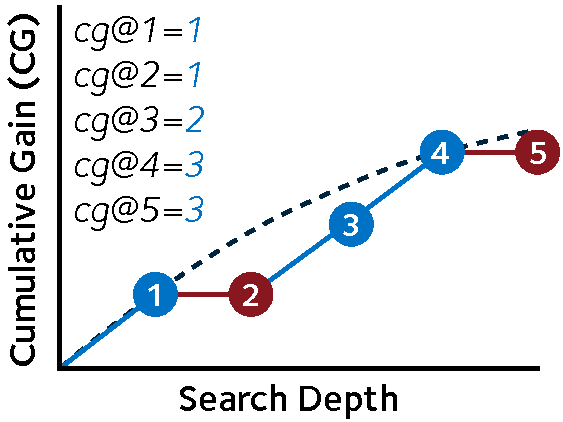
\includegraphics[width=1\textwidth]{figures/ch2-cg.pdf}
    \end{center}
    \vspace*{-4mm}
    \caption[Cumulative Gain]{An illustration of the~\glsfirst{acr:cg} as defined by~\cite{jarvelin2000cg, jarvelin2002cg}. In the example, the first five documents from a list are shown – 1, 3 and 4 contain information, from which the user gains information from. Also pictured is the fitted \emph{gain curve}.}
    \label{fig:cg}
\end{wrapfigure}

Considering the notion of positions within a list of results, a development to~\gls{acr:cg} is~\gls{acr:dcg}. Here, the gain obtained by a new document is discounted according to the rank of that document (i.e. \emph{weighted precision}). A new relevance score is therefore computed for each document by dividing the relevance score by the $log$ of its rank. These discounted scores are then summed, again to a similar cutoff value as described above. This provides an answer to the argument that a document at rank $55$ is less likely to be examined than a document at rank $5$. Even though both may contain relevant information, the perceived worth of the information contained in the document at rank $55$ is reduced to account for its depth in the results. Other measures that are inspired by~\gls{acr:cg} include \emph{Time-Biased Gain (TBG)}~\citep{smucker2012tbg}, a measure that aims to predict the distribution of the number of relevant documents a searcher will save when processing a list of results. 

\subsubsection{Rank-Biased Precision}
Considering on a similar vain to the notion of \emph{weighted precision models}~\gls{acr:rbp}~\citep{moffat2008rbp} is a more contemporary measure that is derived from a simple model of user behaviour. It considers the notion that searchers are not willing to examine every result presented to them. Illustrated in Figure~\ref{fig:rbp}, the underlying user model assumes that a searcher, when presented with a list of results, will always examine the first result, and will examine subsequent documents with a decreasing likelihood (probability $p$), called the \emph{patience} or \emph{persistence} parameter. The searcher's examination of a list will then end with probability $1-p$. Including the patience parameter allows for a very flexible measure to be defined. For example, one can model both persistent (where $p$ tends towards $1.0$) and impatient searchers (where $p\approx0.5$)~\citep{moffat2008rbp}. Indeed, with this flexibility, one can also model the \emph{I'm Feeling Lucky}\texttrademark~button on a Google search, with $p=0.0$ (equivalent to $P@1$).

\begin{figure}[t!]
    \centering
    \resizebox{1\hsize}{!}{
    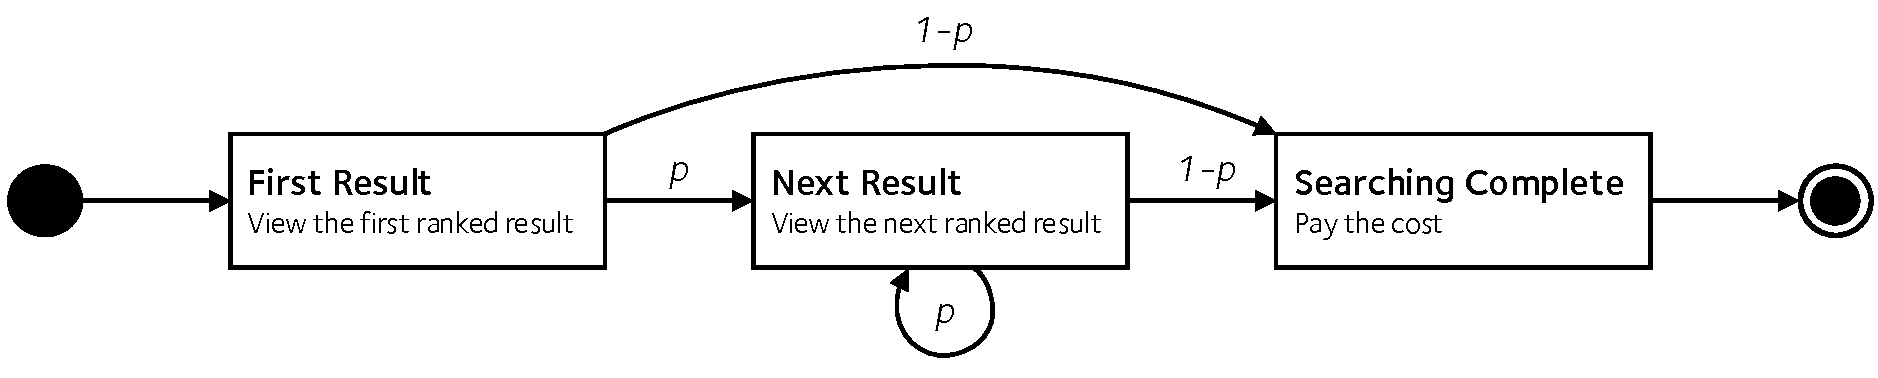
\includegraphics{figures/ch2-rbp.pdf}}
    \caption[Rank-Biased Precision]{An illustration of the simple user model encoded within the~\gls{acr:rbp} measure. A user following this model will \emph{always} examine the first result presented, and will examine subsequent results with decreasing probability (from \emph{p}, the \emph{patience} or \emph{persistence} parameter). Stopping is determined with probability \emph{p-1}. Figure adapted, with permission, from~\cite{moffat2008rbp}.}
    \label{fig:rbp}
\end{figure}

Given a list of documents, $d$,~\gls{acr:rbp} is defined by~\cite{moffat2008rbp} as:

\begin{equation*}
RBP = (1 - p) \cdot \sum_{i=0}^{d}r_i \cdot p^{i-1}.
\end{equation*}

Above, $p$ denotes the patience parameter, with $r_i$ denoting the relevance judgement for a document at rank $i$.~\gls{acr:rbp} has been shown to fit well with actual user data extracted from click logs, as demonstrated in works by~\cite{chapelle2009rbp} and~\cite{zhang2010click_rbp}. Indeed,~\gls{acr:rbp} is used within this thesis as a means for attempting to decide when a simulated user is to stop. By incorporating an additional probability in conjunction with the calculated score at rank $i$, one can then determine, by incorporating some cutoff value $k$, whether a simulated user should stop or continue. Given the success that~\gls{acr:rbp} has had in the literature over the past decade since it was first derived, such a stopping model would be expected to yield good approximations of actual searcher stopping behaviour.

\subsubsection{INST}
The final measure that we consider is the more recently defined \emph{INST} measure, as described by~\cite{bailey2015inst, moffat2015inst}. INST considers the \emph{conditional probability} that a searcher, having examined a document at rank $i$, will examine the next document, at rank $i+1$.


\section{Chapter Summary}
In this chapter, we have introduced some of the key constructs of traditional~\gls{acr:ir}: from indexing documents, to retrieval models, to the ways in which such systems are evaluated. We have also briefly touched on the history of the field, examining some of the manually operated systems that we can today regard as an~\gls{acr:ir} system.

With the focus of this thesis very much on the interactions of users with~\gls{acr:ir} systems, we then turned our attention to the study of~\gls{acr:iir}, detailing a variety of different types of study that can be undertaken in the area. Specifically, we have looked at the basic, underlying user model that are encoded within the Cranfield model (Figure~\ref{fig:trec_model}), and have examined a number of different evaluation measures to help us understand how well users perform. Considering the strong assumptions that the underlying user model poses, the following chapter discusses some of the more complex user models that have been subsequently published in the literature that attempt to carefully deconstruct these assumptions to produce more advanced, realistic means of encapsulating the various processes that take place between a user and system during search.


% Basic concepts -- given a query, tries to satisfy that query.
% Follows a system-orientated methodology
%
% From Leif:
% - indexing
%     tokenizers, etc
% - retrieval models
%     - these models have some notion of how much someone should retrieve/stop.
%     - boolean, look at whole set of documents
%     - other models, there's a cutoff... e.g. cosine similarity, angle gets too large, so you stop.
%     - probabilistic ranking principle
%
%         \begin{quote}
%             ``If a reference retrieval system's response to each request is a ranking of the documents in the collections in order of decreasing probability of usefulness to the user who submitted the request, where the probabilities are estimated as accurately as possible on the basis of whatever data has been made available to the system for this purpose, then the overall effectiveness of the system to its users will be the best that is obtainable on the basis of that data.''
%             \attrib{W.S. Cooper, in private correspondence to~\cite{robertson1977prp}.}
%         \end{quote}
%
%
%         - decreasing probbaility of relevance
%         - get odds of rel over non-rels, so there is some idea of a cut-off.
%         - why would you look at a document that is less relevant?
%         - nobody uses it, just make this observation.
% - evaluation
%     - effects of pooling in judgements?
%     - system orientated (cranfield)
%         - precision
%         - recall
%     - user orientated
%
%     - diane kelly's spectrum of system to user orientated
%         - TREC/Cranfield is a very basic approach to simulation
%             a model of how user performs
%         - user orientated approach looks at how users interact with the system
%         - models of how users search... to show how we develop models.
%
%         - at the end of chapter



% how do people actually interact with a ranked list?
% when do they stop, for example?
%
% we can employ a hybrid approach of conducting user studies to develop a more advanced, TREC++ user model of search.
%
% this model is guided and informed by actual user studies (as discussed in chapters x, y and z).
%
% and then we can test these models out to see whether they are any good by simulating a more advance user, with weaker assumptions, thus moving the area of user modelling forward.







% \subsection{Simulating the User}\label{sec:ir_background:user:simulation}
%
%
% For the purposes of this thesis, we focus upon the studies delineated by categories x and y.
%
%
% central to all of this is the user.
% talk about diane's spectrum of IR experimentation, from system to user focused.
% consider a variety of more user-centric evaluation approaches.
% here, you can also bring in the notion of simulation
% mention that this is IIR.
%
%     - diane kelly's spectrum of system to user orientated
%         - TREC/Cranfield is a very basic approach to simulation
%             a model of how user performs
%         - user orientated approach looks at how users interact with the system
%         - models of how users search... to show how we develop models.
%
%         - at the end of chapter
%
% Look at Kelly (2009) -- Methods for Evaluating Interactive Information Retrieval Systems with Users
%
% these measures/evaluations are thining about the way people go and search
% of relevance to this thesis are stopping strats
% diff. measures encoe different stopping models. different ways of evaluating this.
% in the next chapter, provide an overview of the different types of models of search, and how searching has been conceptualised with respect to stopping strategies.
%
%
%
% \subsection{TREC Ad-Hoc}\label{sec:ir_background:user:trec}
% \todo{does this bit need to be moved to the next chapter?}
% - searcher acquires an information need, sits down, and conducts a search against an existing collection of documents over a set period of time. Known as ad-hoc retrieval, or retrospective searching in older literature.
%
% - this is lifted from Robertson (2008), rephrasing required, and probably needs to be moved to the user model part.
%
% - The user model invoked here is what has now become the most obvious one for search: user has an
% information need, sits down in front of a system and conducts a search against an existing collection of
% documents, over a limited time period. This is known in TREC jargon as an ‘ad-hoc’ search – an earlier more-orless
% equivalent term was ‘retrospective searching’. System produces a ranked list of items, which the user consults
% in rank order. Users may judge documents good or bad, but in principle there may be any number of good
% documents in the collection. (The one significant change in this model from the Cranfield view is that there is now
% an assumption that each system will rank its results list.) It is often asserted that there is also an assumption that
% requests are topical or subject-based (documents about X); indeed the TREC jargon, which is to call requests
% ‘topics’, encourages that view18. However, although most of the requests used in TREC (all of those in early
% TRECs) are indeed topical, there is no necessary requirement of the model that this should be so, or that they
% should be purely topical. In some sense the nature of the requests is determined by the relevance judgements; if
% the judgements depend on other criteria than pure topicality, then that is the nature of the task.
% However, it is fundamental to the model that the judge or assessor should indeed be able to make a judgement
% on each document, actually a binary one for most of the TREC ad-hoc tasks, and should be able to make the
% judgement irrespective of the order of presentation of the documents. This last precludes, for example, embedding
% a criterion of novelty in the usual ad-hoc task relevance judgements (although one track did investigate novelty by
% making judgements of novelty separated from the relevance judgements). A typical TREC ‘topic’ has a short title (which might be used directly as a query), and additional information about the
% supposed information need under the headings ‘description’ and ‘narrative’. The narrative contains explicit rules for
% judging the relevance of documents. An example title and description are: Hydroponics—Document will discuss the
% science of growing plants in water or some substance other than soil.
    %!TEX TS-program = xelatex
%!TEX root = ../../maxwell2018thesis.tex

\chapter[A Background of Stopping in IIR]{Stopping in Interactive\\Information Retrieval}\label{chap:stopping_background}
Towards the end of Chapter~\ref{chap:ir_background}, we examined a number of different evaluation measures typically employed in~\gls{acr:ir} and~\gls{acr:iir} studies. In particular, we emphasised the notion of different \emph{stopping models} that are implicitly encoded within these measures, ranging from the na\"{i}ve to representative approaches encapsulating a real-world searcher's \emph{stopping behaviours.}

\begin{figure}[h]
    \centering
    \vspace{4mm}
    \resizebox{1\hsize}{!}{
    
\includegraphics{figures/ch3-stopsign.pdf}}
    \label{fig:stopsign}
    \vspace{-5mm}
\end{figure}

In this chapter, we provide an overview of work undertaken in the field of~\gls{acr:iir} that examines the stopping behaviours of searchers. We enumerate on a number of different \emph{stopping heuristics} that attempt to quantify when searchers should stop examining results, before examining \emph{theoretical frameworks} that provide insight and explanation into why and when searchers stop. We then examine a number of different \emph{user studies} that have examined stopping behaviour. Before examining these prior works, we first consider why examining the stopping behaviour of searchers is important to the field, and to the future development of the retrieval systems and their interfaces that we use extensively today.

\section{Why Stopping?}\label{sec:stopping_background:why}
Knowing when to stop is a fundamental aspect of human thinking and behaviour. Humans and other animals when interacting with the world will employ some form of \emph{stopping criterion} to decide when they should stop~\citep{nickles1995judgment}. As an example, a shopper who is looking to purchase a new smartphone will stop shopping around once he or she has obtained sufficient information on what new smartphone to purchase. Once their case notes for a patient have been compiled, a medical doctor will then be in a position to diagnose the patient's ailment. In the context of search, numerous reasons exist why searchers stop -- perhaps because they have satisfied their information need, have become frustrated with the lack of potentially relevant information, or because of some external factor, such as a time constraint that has been imposed upon them.

The decision of when to stop is not exclusively due to such external factors to the decision maker, but rather from a series of \emph{internal, cognitive factors} of their thinking process~\citep{nickles1995judgment}. For example, an individual who is hungry will stop eating once he or she is no longer hungry, rather than stopping when all of the food presented to him or her has been consumed. Empirical research has over the years demonstrated that individuals, regardless of the task presented to them, will frequently stop prematurely. Indeed, this na\"{i}ve behaviour demonstrates that individuals may be willing to go with what \emph{``sounds right''} to them -- often minimising the cognitive effort that is required at the expense of greater accuracy~\citep{perkins1983difficulties}. However, when searching, this lower level of potential accuracy does lead to individuals making a greater number of errors in their decision making~\citep{baron1988heuristics}. Searchers overlook important elements, and potentially miss out useful information~\citep{fischhoff1977cost_benefit, fischhoff1978fault, shafir1992thinking}, with the individual then failing to consider alternatives~\citep{farquhar1993decision_structuring}.

Based upon prior research into stopping behaviour, it is clear that such a decision is driven primarily from internal factors. As such, we then consider: \emph{what aspects of the decision maker's thinking processes prompt him or her to stop assessing the information provided?} Knowing when to stop requires that the individual in question makes a \emph{judgement} regarding the sufficiency of the information obtained, and whether or not additional information is required to be obtained~\citep{browne2004stopping_rules}. This judgement is normally characterised by both the completeness and correctness of the information obtained thus far~\citep{smith1991belief}. These claims can be mirrored by qualitative studies on examining stopping behaviour. Here, researchers have found that searchers stop examining search results simply because what they have found previously is \emph{``good enough''}~\citep{zach2005enough_is_enough} to satisfy their underlying information need. This finding echoes the reasoning that individuals would be happy to stop when what they have found \emph{``sounds right''}~\citep{perkins1983difficulties}.

\begin{figure}[t!]
    \centering
    \resizebox{1\hsize}{!}{
    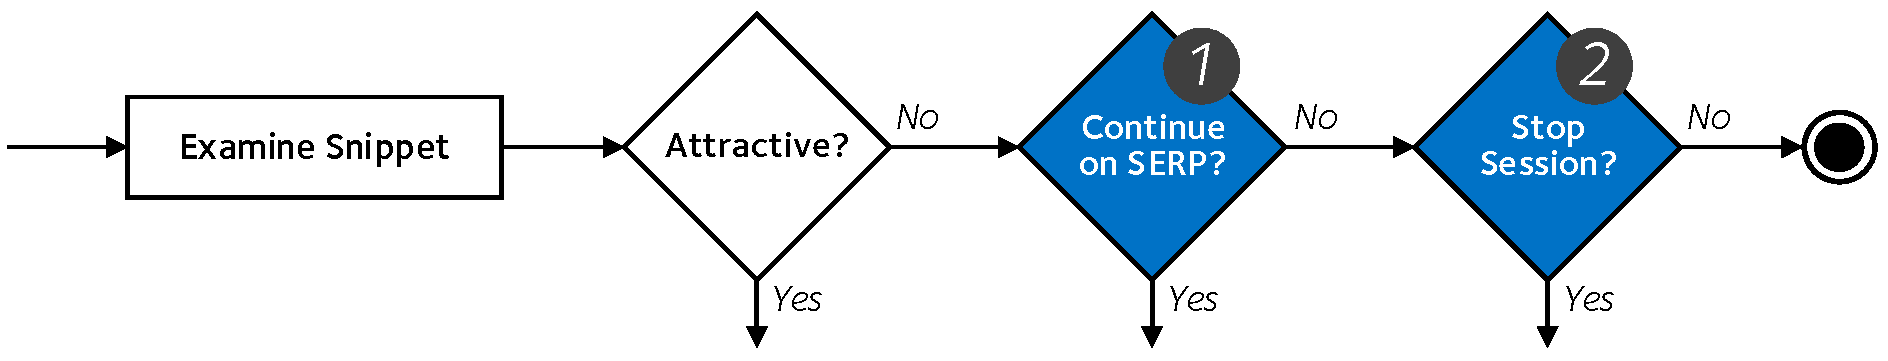
\includegraphics{figures/ch3-two_points.pdf}}
    \caption[Two established \emph{stopping decision points}]{Excerpts from various searcher models, highlighting two established \emph{stopping decision points.} These are modelled as points at which searchers can stop performing a given action. These are illustrated as blue diamonds. The two points consider \blueboxbold{1} \emph{result summary level stopping} (often called \emph{snippet level} or \emph{query level stopping}), and \blueboxbold{2} \emph{session level stopping}.}
    \label{fig:model_two_points}
\end{figure}

\subsection{Stopping Decision Points}\label{sec:stopping_background:why:points}
In Section~\ref{sec:ir_background:user:models}, we discussed a number of searcher models that are considered an improvement over the traditional~\gls{acr:trec}-style searcher model, a model that is agnostic of a searcher's interactions. These more advanced models considered two distinct \emph{stopping decision points} that capture specific points during the interaction process where a searcher can stop their current activity, and move onto the next step in the process.

These stopping decision points are illustrated in an excerpt of a typical searcher model flowchart, as shown in Figure~\ref{fig:model_two_points}. Below, each of the stopping decision points are enumerated.

\vspace*{-4mm}
\begin{itemize}
    \item[\blueboxbold{1}]{\blueboxbold{Result Summary Level Stopping} Traditionally called \emph{snippet level stopping} or \emph{query level stopping} in the literature\footnote{The phrase \emph{result summary level stopping} is used in this thesis to avoid confusion with a new~\gls{acr:serp} level stopping decision point, discussed in more depth in Section~\ref{sec:csm:advancements:stopping}.}, this stopping decision point concerns the depth at which a searcher will stop examining a list of ranked results. After stopping at this point, the searcher can continue the search session by issuing a further query.}
    \item[\blueboxbold{2}]{\blueboxbold{Session Level Stopping} This final stopping decision point considers the point where a searcher will stop their search session in its entirety. As such, this stopping decision point is regarded as \emph{terminal} to the search session.}
\end{itemize}
\vspace*{-4mm}

In particular, session level stopping is considered when a searcher must decide, for example, if they have met their overall search goal, have run out of time or queries, or simply have become so frustrated with a lack of relevant content that they would rather abandon the search. These stopping decision points can be operationalised in a variety of different ways, as we explore in the remainder of this chapter. Chapter~\ref{chap:csm} also proposes an additional, third stopping decision point that we will consider in later contributory chapters of this thesis.

\section{Stopping Heuristics}\label{sec:stopping_background:heuristics}
Considering the above, researchers have over a number of decades devised a number of different high level \emph{stopping rules} -- hereafter referred to as \blueboxbold{stopping heuristics} -- as a means of encoding a searcher's aforementioned sense of what is \emph{``good enough''}~\citep{zach2005enough_is_enough} -- or, indeed, what can be considered to be \emph{not good enough,} too.

Stopping heuristics have been investigated in \emph{decision making} research. A number of normative stopping heuristics have been identified. As examples of such heuristics,~\cite{busemeyer1988deferred_decision_making} considered the expected loss from terminating information acquisition.~\cite{kogut1990sunk_costs} examined the expected value of additional information. Other examples of normative stopping heuristics are demonstrated by~\cite{pitz1969information_seeking} and~\cite{busemeyer1988deferred_decision_making}.

However, as outlined by~\cite{browne2004stopping_rules}, these heuristics usually fail to describe the actual cognitive behaviours of the decision makers. Such heuristics often assume that the decision maker must \emph{think ahead} to the final decision of when to stop, enabling them to assess the value of additional information~\citep{busemeyer1988deferred_decision_making}. This is however an inherently difficult task for decision makers to undertake, due to the limited working memory capacity of a human. We are simply unable to hold and evaluate all of the information attained to make a decision considering all possible outcomes~\citep{browne2004stopping_rules}.~\cite{nickles1995judgment} agreed, stating that normative stopping heuristics made implicit assumptions about the mental activities of the decision maker, especially in terms of mental scaling and weighting. No clear cognitive perspective is provided to address the assumptions of the decision maker's thinking.

With these inherent limitations in mind, seminal work in this area was undertaken by~\cite{nickles1995judgment} who provided a broad classification for different explicitly defined stopping heuristics in the literature. These heuristics consider a searcher's cognitive processes, and are considered as either \emph{judgement-based heuristics} and \emph{reasoning-based heuristics.} The heuristics we consider are enumerated below, split across the two aforementioned classifications.

\begin{itemize}
    \item{\darkblueboxbold{Judgement-based Heuristics} These heuristics are defined as when a decision maker maintains some mental threshold along a key dimension, and a running total of the number of occurrences of this measure. More details are provided in Section~\ref{sec:stopping_background:heuristics:judgement}.}
    \begin{itemize}
        \item{\blueboxbold{Satisfaction and Frustration} These heuristics consider a decision maker's satisfaction with what they have found during the course of their search \emph{(satisfaction),} or their tolerance to non-relevance \emph{(frustration).}}
        \item{\blueboxbold{Magnitude Threshold} This heuristic concerns a decision maker's belief that the information that they have found provides sufficient evidence to prompt him or her to stop searching for further information.}
        \item{\blueboxbold{Difference Criterion} This heuristic concerns the notion of whether a decision maker is learning anything new with more documents.}
        \item{\blueboxbold{Single Criterion} A \emph{single criterion} to the decision maker's information need is considered in this stopping heuristic.}
    \end{itemize}
    
    \item{\darkblueboxbold{Reasoning-based Heuristics} This classification of heuristic concerns the \emph{mental representation} of the given topic that a searcher is examining information for.}
    \begin{itemize}
        \item{\blueboxbold{Representational Stability} This stopping heuristic concerns the notion of the decision maker's mental model of the topic, and the \emph{stabilisation point.}}
        \item{\blueboxbold{Propositional Stability} Here, a series of potential conclusions regarding the underlying information need are formed, with these arguments needing to be satisfied to stop.}
        \item{\blueboxbold{The Mental List} A mental list of aspects is constructed, with each item on the list needing to be addressed by the decision maker before stopping occurs.}
    \end{itemize}
\end{itemize}

These were devised largely as ways of modelling the~\glsfirst{acr:esl}~\citep{cooper1968expected_search_length}, as briefly discussed in Section~\ref{sec:ir_background:evaluation:system:esl}.~\cite{nickles1995judgment} also proposed a number of stopping heuristics that are discussed in subsequent sections, with discussion expanded to included additional heuristics defined by other researchers. We now address each of the two classifications, explaining each of the different heuristics enumerated above in detail.

\subsection{Judgement-Based Heuristics}\label{sec:stopping_background:heuristics:judgement}
As discussed previously, a judgement-based stopping heuristic is defined as when a decision maker is assumed to set and consistently maintain a mental threshold along some form of key dimension (e.g. determining the seemingly relevant from non-relevant), and to keep a running total of measure relative to the dimension in question~\citep{gettys1979hypothesis, nickles1995judgment}. When the measure is met or exceeded this set threshold, the searcher will then stop their searching activity. Each of the judgement-based heuristics we consider in this thesis are discussed in turn below.

\subsubsection{Satisfaction and Frustration}\label{sec:stopping_background:heuristics:frustration}
Two of the earliest stopping heuristics defined in the literature are by~\cite{cooper1973retrieval_effectiveness_ii} which consider a searcher's tolerance to relevant and non-relevant material. The heuristics were originally defined as a means for estimating the utility a searcher can attain when interacting with a retrieval system. While the means of which~\cite{cooper1973retrieval_effectiveness_ii} estimated the utility of search are not of key relevance to this thesis, the work on stopping heuristics are. The \emph{satisfaction point} and \emph{frustration point} stopping heuristics are considered to be judgement-based heuristics as they rely solely on the searcher's notion of what constitutes a relevant document -- and both consider counts of the number of (non-)relevant documents observed.

\blueboxheader{Satisfaction Point}
Given the name, it is not surprising that the \emph{satisfaction point} heuristic considers the point at which a searcher has found enough perceived relevant material to consider his or her search a success. It can be easily imagined that such a heuristic would apply directly to both result summary level stopping (i.e. \emph{find $x$ relevant documents on this SERP}) and session level stopping (i.e. \emph{find $x$ relevant documents}). This heuristic is also called the \emph{satiation heuristic}~\citep{simon1955satiation} (see below). This heuristic can be considered as a decision making process...

\begin{quote}
    \emph{``[...]through which an individual decides when an alternative approach or solution is sufficient to meet the individuals' desired goals rather than a perfect approach.''}
    \attrib{\cite{simon1971decision}}
\end{quote}

This essentially suggests that a searcher employing this particular heuristic would stop searching as soon as certain conditions arise, instead of after they have exhaustively considered all available information~\citep{march1994primer}. Conditions could include acceptance of the results, discomfort, boredom, time limits and the \emph{snowballing} of information~\citep{mansourian2007search}.

\blueboxheader{Frustration Point}
In a converse fashion to the satisfaction point heuristic, the \emph{frustration point} heuristic considers a searcher's overall \emph{tolerance to non-relevance} by stopping after being sufficiently frustrated by the results presented to the searcher. This heuristic is also called the \emph{disgust heuristic} in the literature (see below).

The two relatively straightforward heuristics defined above makes a searcher's interactions with a ranked list of results \emph{inherently adaptive.} In other words, given a set of results, his or her behaviour will change with respect to the perceived quality of the ranked list. As a reminder, this would not necessarily mean considering the system's effectiveness measures, but rather user-focused measures such as interactive precision and recall, as discussed previously in Section~\ref{sec:ir_background:evaluation:user:ipr}.

\blueboxheader{Combining Satisfaction and Frustration}
Perhaps due to the relative simplicity of two aforementioned heuristics, identical approaches have also been defined elsewhere in the literature.~\cite{kraft1979stopping_rules} later defined three further stopping heuristics, two of which are the \emph{satiation} (as per~\cite{simon1955satiation}) and the somewhat loaded \emph{disgust} heuristics. In essence, the rules defined by~\cite{kraft1979stopping_rules} are the same satisfaction and disgust heuristics as previously defined by~\cite{cooper1973retrieval_effectiveness_ii}. Within the satiation rule, a searcher will stop after been \emph{satiated} by finding a number of documents considered to be relevant, while the disgust rule considers a searcher's disgust at finding a number of non-relevant documents.

\cite{kraft1979stopping_rules} also proposed a third heuristic that \emph{combines} both the satisfaction/satiation and frustration/disgust rules together into a single heuristic. Here, a searcher following such an approach would be inclined to stop examining content if they were either satisfied with what had been found, or frustrated by having to trawl through a number of material judged to be non-relevant. The stopping point would be whatever of the two conditions are met first. Indeed,~\cite{kraft1979stopping_rules} demonstrated that the~\gls{acr:esl} of a searcher could be approximated using each of the two stopping heuristics by considering the size of the retrieval set, the number of relevant documents a searcher wished to obtain, and the number of non-relevant documents a searcher would be willing to tolerate. The number of documents required to consider a search as successful is dependent upon whether the search task is high precision (where one would stop comparatively early) or high recall (where one would stop comparatively later), as hypothesised by~\cite{bates1984thirty_items}.

\subsubsection{Magnitude Threshold}\label{sec:stopping_background:heuristics:magnitude}
\begin{wrapfigure}[11]{r}{0.45\textwidth}
    \begin{center}
    \vspace*{-10mm}
    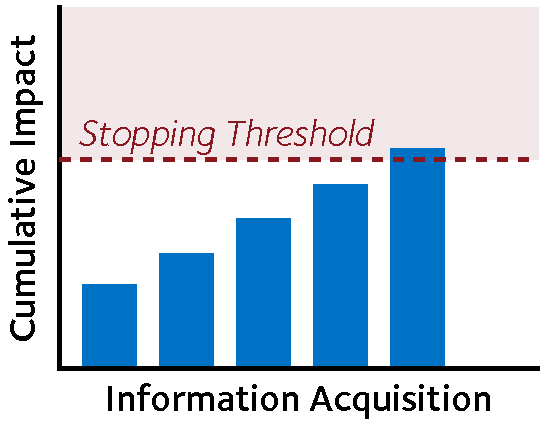
\includegraphics[width=1\textwidth]{figures/ch3-threshold.pdf}
    \end{center}
    \vspace*{-6mm}
    \caption[The magnitude threshold stopping heuristic]{The magnitude threshold heuristic. Once a searcher accrues a predetermined level of impact, he or she stops. Adapted from~\cite{browne2004stopping_rules}.}
    \label{fig:threshold}
\end{wrapfigure}

The magnitude threshold heuristic~\citep{nickles1995judgment} considers an individual's belief that the information accrued during the search process provides \emph{sufficient evidence} to prompt him or her to stop searching for further information. The point at which the searcher would decide to stop is determined by some predetermined, internal threshold that must be reached, which acts as the stopping criterion~\citep{wald1948sequential_analysis, nickles1995judgment}.~\cite{gettys1979hypothesis} hypothesise that the searcher \emph{`mentally tabulates'} the cumulative impact of the evidence that he or she has uncovered, and when the internal tabulation crosses the specified threshold, he or she stops.

Determining what exactly this threshold should be before commencing a task has attracted research from several perspectives. Indeed, this decision can be left open to interpretation by the individuals who choose to operationalise such a heuristic. However, research has shown that under different tasks, varying the criteria by which an individual bases their initial threshold value varies. For example,~\cite{busemeyer1982choice_behaviour} demonstrated this for decision making under uncertainty.~\cite{saad1996stopping} demonstrated the usefulness of this heuristic under common choice tasks.

An abstract representation of the stopping heuristic is provided in Figure~\ref{fig:threshold}. From the figure, we can see that a searcher accrues information through each document that is examined. This is combined together to form a \emph{cumulative impact} of the information. For each document examined, the current cumulative impact value is compared against a predetermined threshold value. If the cumulative impact is above this threshold, the searcher then assumes that enough supporting evidence has been collected, and stops.

\subsubsection{Difference Threshold}\label{sec:stopping_background:heuristics:difference}
The \emph{difference threshold heuristic}~\citep{nickles1995judgment} concerns whether a new document is teaching a searcher anything new about their information need, or the marginal value of the latest document. Here, the searcher is assumed to keep an internal record of the information that has been consumed along some key dimension. The searcher is also assumed to use this internal record of what has been assessed to compare a new document with previously examined content. When the difference between the new and existing information falls below some internal difference threshold, the searcher stops as nothing new is being learnt.

\begin{figure}[t!]
    \centering
    \resizebox{1\hsize}{!}{
    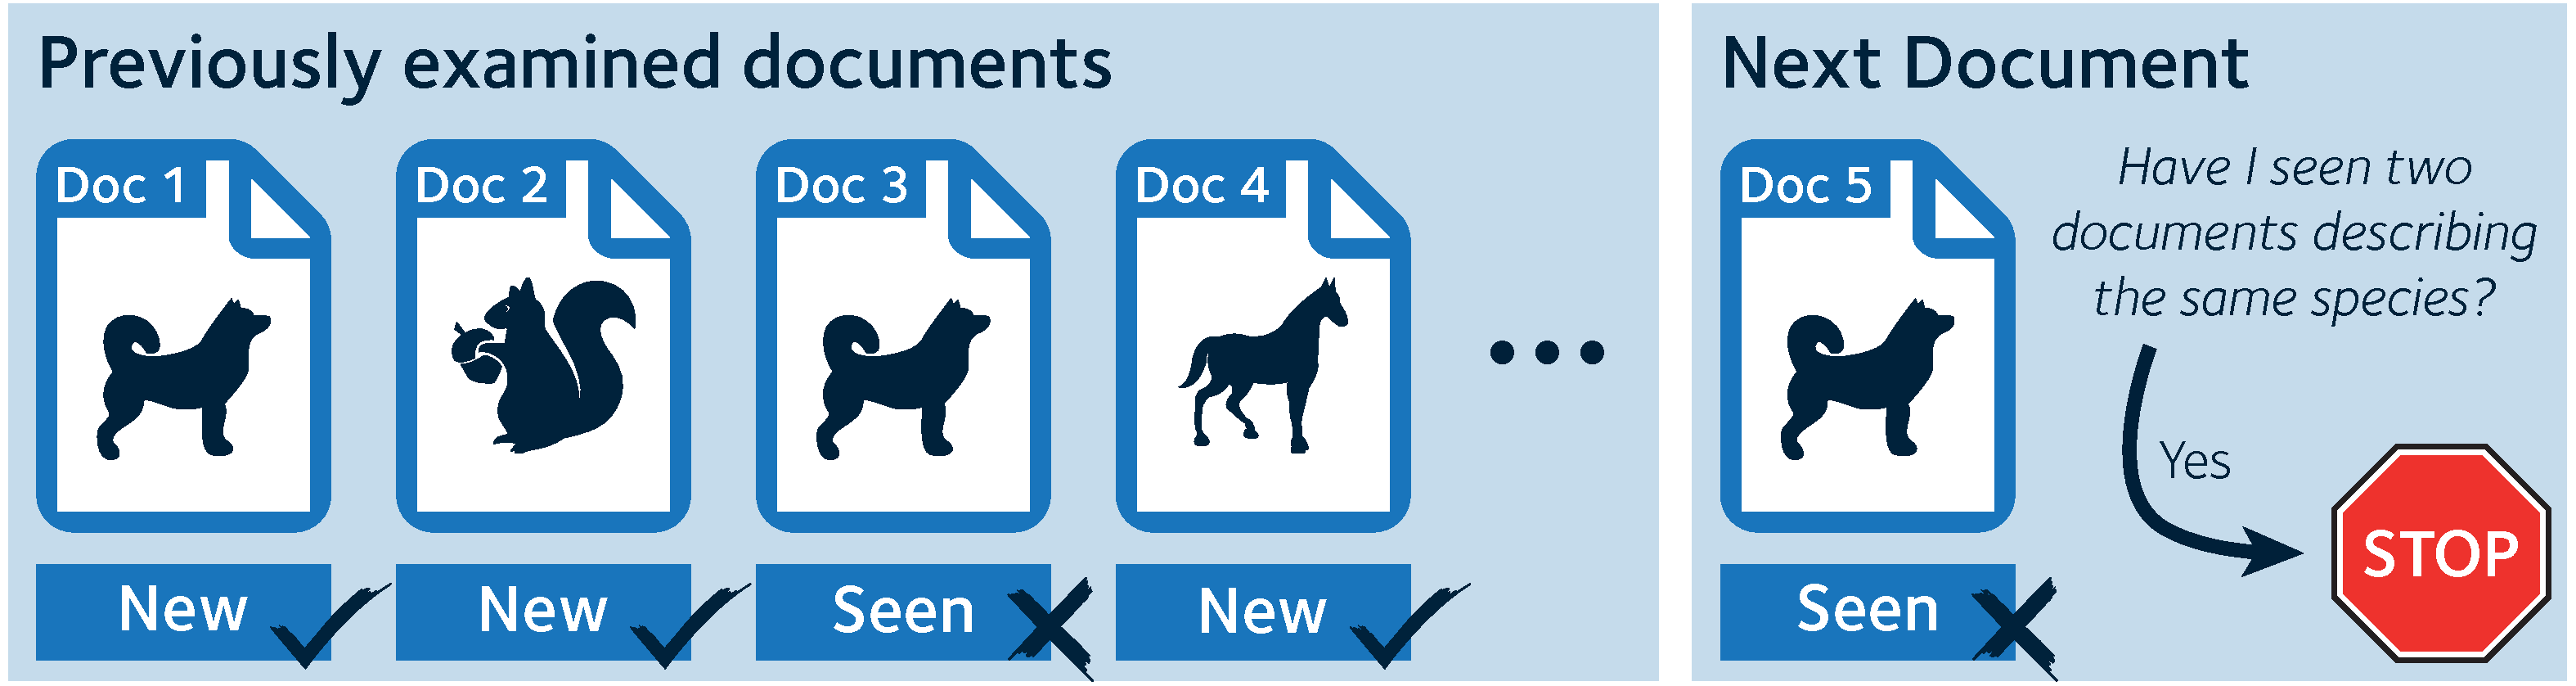
\includegraphics{figures/ch3-difference.pdf}}
    \caption[Difference threshold heuristic]{A simplified, visual example of the difference threshold heuristic. Given the information need of finding different species of animal, a searcher issues a query, and examined a number of documents. The third document offers information on dogs, which has been already observed in \emph{Doc 1.} Using the stopping criterion that once the same species has been observed twice, \emph{Doc 5} satisfies it. This then means that the threshold has been met, and the searcher then stops.}
    \label{fig:difference_heuristic}
\end{figure}

As a crude example of this heuristic, a searcher is provided with an information need to find as many different species of animal as possible. Once a query has been issued, the searcher begins to examine documents on the SERP. This is illustrated in Figure~\ref{fig:difference_heuristic}, where the first document considers dogs. A simple criterion is employed whereby the searcher stops after encountering the same animal twice, illustrating that nothing new is being learnt from the list of results presented. Once this is met, the searcher abandons the SERP, and can then perform a query reformulation to discover different species of animal.

\subsubsection{Single Criterion}\label{sec:stopping_background:heuristics:single}
The \emph{single criterion heuristic} was later defined by~\cite{browne2005stopping_rules}. As the name suggests, this heuristic considers a searcher examining information for a \emph{single criterion} related to their information need, typically assumed to be the most important one. The searcher then stops examining content once he or she has deduced that enough information about said criterion has been accumulated for them to be satisfied. The concept of a stopping threshold can be borrowed from the magnitude threshold heuristic, discussed in Section~\ref{sec:stopping_background:heuristics:magnitude}. This considers that a searcher will stop once they have accumulated enough impactful information.

\cite{browne2005stopping_rules} go on to provide an example search task where the single criterion threshold would be directly applicable. When purchasing a mortgage for a new house, a searcher will explore the websites of various mortgage lenders in order to find the best deal for them. Given a mortgage deal, the most obvious criterion that an individual would look for would be interest rates, with the lower the rate, the more attractive the deal. Of course, other factors may influence the decision, but this example ultimately demonstrates how the heuristic works in simple terms.

\subsection{Reasoning-Based Heuristics}\label{sec:stopping_background:heuristics:reasoning}
The second category of stopping heuristics as defined by~\cite{nickles1995judgment} are \emph{reasoning based}. While searching and accruing information about a particular topic, a searcher is essentially developing a mental representation of the topic~\citep{yates1990decision_making}. As argued by~\cite{nickles1995judgment}, these elements can include arguments constructed during informal reasoning, previously constructed arguments, or information evoked from the searcher's long term memory. As such,~\cite{nickles1995judgment} devised a category of stopping heuristics that are dominated by the searcher's reasoning processes.

\subsubsection{Representational Stability}\label{sec:stopping_background:heuristics:representational}
\begin{wrapfigure}[8]{r}{0.45\textwidth}
    \begin{center}
    \vspace*{-11mm}
    
\includegraphics[width=1\textwidth]{figures/ch3-representational.pdf}
    \end{center}
    \vspace*{-5mm}
    \caption[Representational stability stopping heuristic]{A crude illustration of the representational stability stopping heuristic. The searcher's model of the given information need begins to stabilise at \emph{t-1}, meaning that a searcher would stop at \emph{t}.}
    \label{fig:representational_heuristic}
\end{wrapfigure}

The representational stability heuristic~\citep{nickles1995judgment} (with the phenomenon initially discussed by~\cite{yates1982toward}) concerns the notion that as a searcher acquires new information, his or her mental model of the underlying information need shifts and develops -- but only up to a certain point. From this point onwards, their mental model stabilises and the searcher is said to have accrued enough information to satisfy or understand the (sub)topic.

It is stated by~\cite{nickles1995judgment} that while a searcher examines content, he or she generates arguments that serve to develop and elaborate his or her conception of the decision(s) that they are tasked to make. As the searcher continues to reason, certain arguments may be relegated to long term memory due to the limited size of the searcher's working memory. Searchers will accrue new information, with some perhaps returning to the original subset of arguments. As mentioned previously, it is at this point that can be interpreted as a form of stability regarding the information need. This is depicted in Figure~\ref{fig:representational_heuristic}, where given a vague information need, a searcher will trawl a series of documents in order to develop their mental model of the given problem, turning their understanding of the topic from an initial \emph{fuzzy} state to \emph{crystal clear.}

\subsubsection{Propositional Stability}\label{sec:stopping_background:heuristics:propositional}
Similar to the representational stability heuristic,~\cite{nickles1995judgment} also defined the \emph{propositional stability} heuristic which again focuses on the concept of a stabilising mental model of the given information need. Here, a searcher when examining content will form a series of arguments from the information he or she is observing. These arguments can lead to \emph{tentative conclusions}, from which at some point stability is achieved, and the conclusion does not change. This heuristic therefore suggests that the stabilised nature of the decision maker's conclusion from the information observed prompts him or her to stop.

\subsubsection{The Mental List}\label{sec:stopping_background:heuristics:mental}
The mental list stopping heuristic considers a mental list of aspects of some phenomenon. Each of the different aspects within the mental list must be \emph{`checked off'} to a satisfactory level before the searcher then decides to stop examining content. This mental list can typically be constructed from a searcher's long term memory, meaning that they will likely have \emph{a priori} knowledge of the particular information need. So-called belief structures such as \emph{schemas}~\citep{bartlett1933remembering} or \emph{scripts}~\citep{schank1977scripts} may assist the searcher in organising the construction of the mental list that forms the set of criteria that determines when they stop.

Figure~\ref{fig:mental_list} provides a graphical illustration of the mental list heuristic. When looking for a new car, a searcher will construct a mental list of different aspects of a car which are essentially the minimum requirements (e.g. a minimum engine displacement of 1.8 litres). Searching is then conducted, with the searcher narrowing down the potential choices available to them to those that satisfy their mental list.

\begin{figure}[t!]
    \centering
    \resizebox{1\hsize}{!}{
    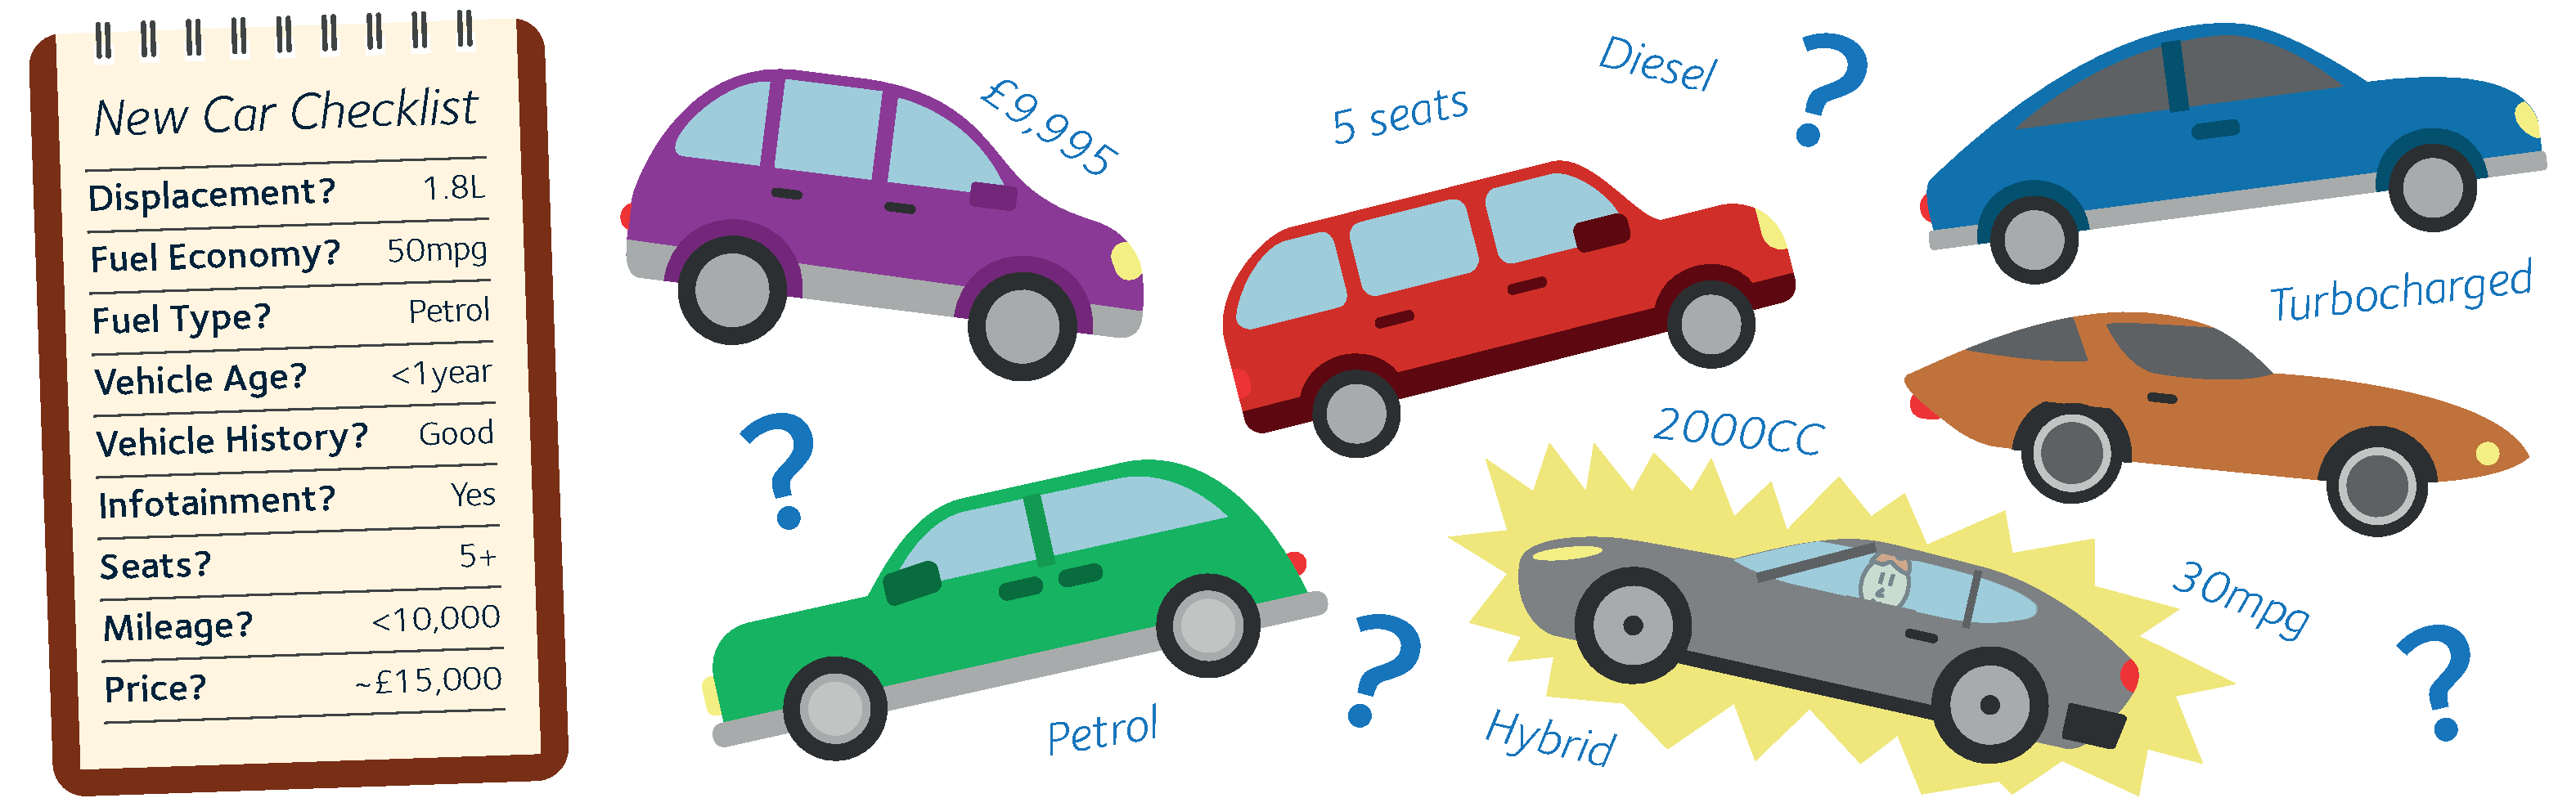
\includegraphics{figures/ch3-mental_list.pdf}}
    \caption[The mental list stopping heuristic]{Given a well defined information need,~\cite{nickles1995judgment} defined the mental list heuristic – where a number of different criteria must be satisfied before stopping. In the illustration above, car shopping is used as an example. Here, certain criteria for a new car (as shown on the notepad) must be met before a searcher is satisfied with what they have found.}
    \label{fig:mental_list}
\end{figure}

\subsection{Summary of Heuristics}
In this section, a number of different stopping heuristics have been discussed from a number of seminal papers in the literature. While a much larger of number of normative stopping heuristics have been defined in prior works, these have been omitted from the review as they do not adequately describe the cognitive behaviours of a searcher, often assuming a searcher has to \emph{think ahead} to make a decision to stop or continue~\citep{browne2004stopping_rules}. In contrast, the heuristics that are enumerated above do not make this assumption, making more realistic assumptions about the searcher's cognitive abilities.

Of course, the different stopping heuristics discussed above are likely to behave differently under different search contexts. As an example, the mental list heuristic might be impossible to use given a searcher with a very limited knowledge of a topic. He or she simply would not know enough information to ascertain key aspects of the topic, and construct a set of criteria that must be met~\citep{browne2005stopping_rules} --~\cite{gigerenzer1999betting} also discuss this reasoning for the single criterion heuristic. As such, it is hypothesised that the aforementioned stopping heuristics would be likely to work better with a searcher who is more knowledgeable.

%Indeed,~\cite{browne2005stopping_rules} hypothesises that magnitude threshold and mental list heuristics would be best applied to searchers with a greater degree of understanding of the topic.

\cite{browne2005stopping_rules} also discuss the so-called \emph{``structuredness''} of a given search task. If the task has well defined inputs and outputs -- or the goals and operations are clear and easily understood~\citep{simon1996sciences} -- then it it hypothesised that searchers will employ more precise stopping heuristics for deducing when to stop. For example, the mental list and single criterion stopping heuristics might offer greater degrees of precision than for example the frustration and satisfaction heuristics, although the frustration and satisfaction heuristics may perform well for any given search task. Altogether however, the heuristics discussed in this section would be applicable for informational search tasks~\citep{browne2005stopping_rules}, such as ad-hoc retrieval (refer to Section~\ref{sec:ir_background:paradigms:trec}).

With the heuristics now enumerated, we later in this thesis discuss how we take these stopping heuristics, and consider how to \emph{operationalise} them, such that they can be subsequently implemented and compared against each other empirically. This also involves which of the three stopping decision points we discussed in Section~\ref{sec:stopping_background:why:points} these operationalised heuristics can be used in. Chapter~\ref{chap:strategies} provides a complete set of the twelve \emph{stopping strategies} that we employ in the contributory work in this thesis.

\section{Theoretical Models}\label{sec:stopping_background:theoretical}
In addition to the stopping heuristics above, mathematically grounded, theoretical models have been defined that allow us to describe, predict and explain \emph{how} and \emph{why} searchers behave in the way they do. Crucially for this thesis, such models provide an explanation of their stopping behaviour. As discussed in Section~\ref{sec:ir_background:user:simulation} however, such models also have limitations, ranging from the low level assumptions engaged by the different models, the variables that are considered or excluded from the models, and the difficulties arising from the complexities of human behaviour~\citep{fishwick1995simulation, azzopardi2015theories}.

Despite the limitations of such an approach, such \emph{formal models} also permit the generation of different hypotheses regarding search behaviours. These can subsequently empirically tested and validated -- with examples including~\cite{azzopardi2013query_cost} and~\cite{pirolli1996scatter_techniques}. Three examples of such theories include~\glsfirst{acr:ift}~\citep{pirolli1999ift},~\glsfirst{acr:set}~\citep{azzopardi2011economics} and the~\glsfirst{acr:iprp}~\citep{fuhr2008iprp}. Central to the work in this thesis is~\gls{acr:ift} that we discuss in detail in the following subsection. As shown by~\cite{azzopardi2015theories} however, the three theories are all mathematically equivalent, with all demonstrating the same understanding. As such, we do not discuss~\gls{acr:set} and~\gls{acr:iprp} in detail.

%As such, this section focuses on a discussion of~\glsfirst{acr:ift} as a means for explaining a searcher's \emph{optimal stopping behaviour.} We also briefly acknowledge two other competing theoretical models of search.

\subsection{Information Foraging Theory}\label{sec:stopping_background:theoretical:ift}
A well known conceptual model in the field of information seeking is the \emph{berry picking model}, as proposed by~\cite{bates1989berry_picking}. As shown in Figure~\ref{fig:berry_picking}, this model considers searchers looking for information to be analogous to \emph{foragers} scavenging for food in the wild. In the model, foragers are looking for the juiciest and ripest berries on a number of different \emph{patches}, or bushes. The juiciest and ripest berries offer the highest levels of gain. Picking these berries helps the forager maximise their level of gain. Applied to search, this construct means that a searcher \emph{forages for information,} picking the most relevant (or juiciest) documents that help them maximise their level of gain.

While the berry picking model is an intuitive and simple model to understand, its highly descriptive nature does not provide an explanation regarding the behaviour of the forager. \emph{How long should a forager spend examining this berry bush?} This question cannot be answered as such by the model, but~\cite{bates1989alluding} in a later publication does allude to the fact that searchers could weigh up the costs and benefits in order to decide what to do next.

Theories do however exist that attempt to explain the behaviour of a searcher when \emph{foraging} for information. Initial attempts by~\cite{russell1993sense_making} and~\cite{sandstrom1994optimal_foraging} demonstrated that~\glsfirst{acr:oft}~\citep{stephens1986foraging_theory} could be potentially used to model the search process. This led to the development of~\glsfirst{acr:ift}, proposed by~\cite{pirolli1999ift}. The theory provides an explanation as to how information foragers will behave, and as such, also provides a rationale as to how they will \emph{stop.}~\gls{acr:ift} is extensively used in this thesis as a theoretical underpinning to several hypotheses. We also outline an optimal stopping heuristic, as well as several other time-based heuristics that derive from~\gls{acr:oft}.

\begin{figure}[t!]
    \centering
    \resizebox{1\hsize}{!}{
    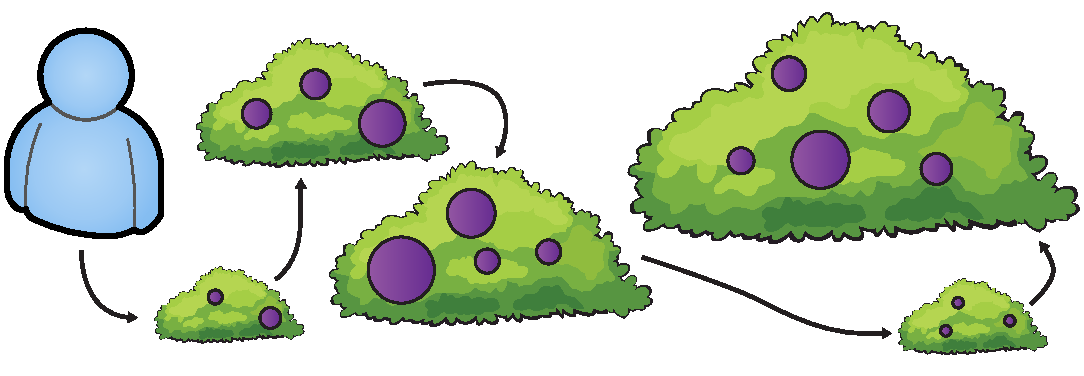
\includegraphics{figures/ch3-berry_picking.pdf}}
    \caption[The Berry Picking Model~\cite{bates1989berry_picking}]{The \emph{Berry Picking Model,} defined by~\cite{bates1989berry_picking}. A forager traverses through numerous bushes to pick the juiciest berries for his or her consumption. The model is high level and conceptual in nature, and thus does not provide any justification for \emph{how} or \emph{why} foragers search for the juiciest berries.}
    \label{fig:berry_picking}
\end{figure}

\subsubsection{Patches and Scent}\label{sec:stopping_background:theoretical:ift:patch}
\gls{acr:ift} is comprised of three main models: the \emph{information diet model}, concerning \emph{what} information is consumed; the \emph{information patch model}; and the \emph{information scent model.} With the information diet model not considered in this thesis, we focus in this section on discussing the information patch and information scent models.

Central to~\gls{acr:ift} is the notion of a \emph{patch}, as per the patch model. In the wild, a patch is modelled as an area of land with a degree of potential gain (food) that can be acquired by foraging through said patch. The \emph{between patch time} is the amount of time a forager spends moving towards a patch, and the \emph{within patch time} is the time spent within the patch, examining its contents for potential gain.

With~\gls{acr:ift}, a patch can be modelled in a variety of ways. However, as outlined by~\cite{azzopardi2015theories}, the generally agreed approach to model a patch in terms of information seeking is to consider it as a~\gls{acr:serp}. With this representation, moving between a patch is akin to \emph{issuing a query,} and thus incurs a cost (between patch time), and staying within a patch is the same as assessing result summaries on the presented~\gls{acr:serp} and their associated documents, with each summary and/or document taking a certain amount of time to process (the within patch time). The patch model essentially predicts how long an information forager should stay in a patch before abandoning it and moving to the next patch.

However, given a series of patches, how does a forager deduce which one he or she should \emph{enter} next, and examine in closer detail? This is described by the information scent model, and encapsulates a currently active area of research. Figure~\ref{fig:patch_model} graphically illustrates the scent of a patch in action -- given two patches as depicted in the illustration, what patch will the forager travel to next? Following the scent, or \emph{cues} on the ground next to him, the forager observes that the paw prints to the first patch are more prevalent, and thus will venture to that patch first. Like foragers in the wild, information foragers will observe a series of \emph{proximal cues} presented to them on a~\gls{acr:serp}, such as hypertext links, document titles, snippet text and thumbnails to locate information~\citep{pirolli1995ift, pirolli1999ift, chi2001information_scent, oltston2003scenttrails, pirolli2007ift}. In the context of news search, cues were examined by~\cite{sundar2007news_scent}. Here, cues such as the source of an article were shown to have a powerful effect on the perception of said article.

If these cues provide a rationale as to what leads to a promising scent trail, it follows that scent, in combination with patches, provides a rationale as to when a searcher will stop examining a set of results~\citep{pirolli1999ift, wu2012dc, wu2014information_scent}. For example, a user study by~\cite{wu2014information_scent} demonstrated that a searcher would forage to greater depths if the~\gls{acr:serp} appeared to contain many relevant items. This trend was also observed by~\cite{card2001scent_graphs}, who found that when navigating through webpages, searchers were more likely to leave when the information scent began to decline. Section~\ref{sec:stopping_background:user_studies} provides more details on these user studies, along with others considering stopping behaviours.

\begin{figure}[t!]
    \centering
    \resizebox{1\hsize}{!}{
    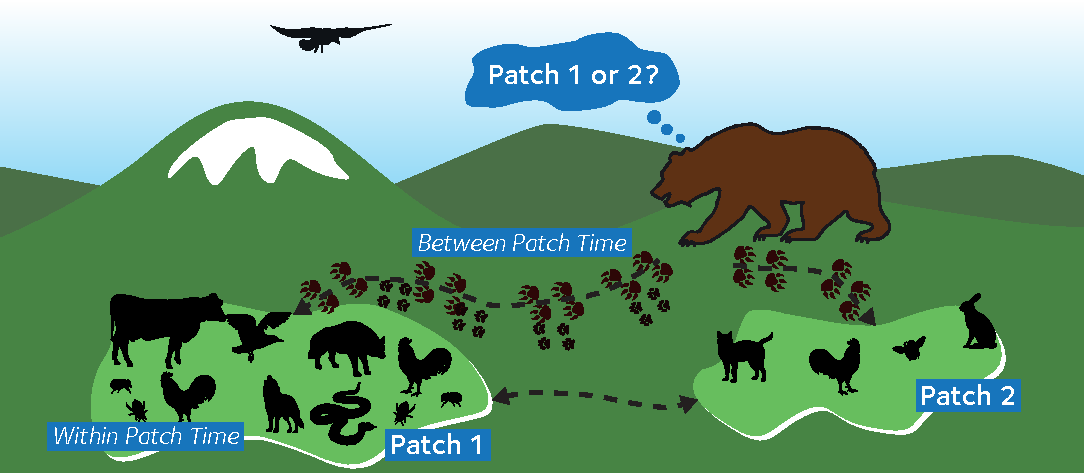
\includegraphics{figures/ch3-patch.pdf}}
    \caption[The patch model]{A graphical depiction of the \emph{Patch Model}, part of ~\glsfirst{acr:ift}. When presented with two patches, each containing food that can be represented as gain, what patch should our forager choose first — patch \raisebox{-.2\height}{
\includegraphics[height=5mm]{figures/ch2-point1.pdf}} or \raisebox{-.2\height}{
\includegraphics[height=5mm]{figures/ch2-point2.pdf}}?}
    \label{fig:patch_model}
\end{figure}

\subsubsection{Stopping Heuristics}\label{sec:stopping_background:theoretical:ift:stopping}
Given a patch with a scent, how can one deduce \emph{when they should stop?} Like all theories,~\gls{acr:ift} makes some key assumptions from which we can deduce behavioural characteristics of a forager. The assumptions are that a forager will:

\begin{itemize}
    \item{enter a patch with what appears to be the highest yield first; and}
    \item{attempt to maximise their gain per unit of time.}
\end{itemize}

Given these assumptions, one would now be able to answer the question posed in the graphical illustration of patches in Figure~\ref{fig:patch_model}. With the better scent, and greater volume of potential energy to be gained, the first patch is the obvious answer that a forager would answer to the question: \emph{which patch should I explore first?}

In addition, the assumptions provided above allow us to begin formulating a stopping heuristic based upon the \emph{optimal behaviour} of a forager. The~\gls{acr:mvt} by~\cite{charnov1976mvt} states...

\begin{quote}
    \emph{``...that a forager should remain in a patch so long as the slope of the gain function is greater than the average rate of gain in the environment.''}
    \attrib{\cite{pirolli1999ift}}
\end{quote}

\begin{wrapfigure}[12]{r}{0.45\textwidth}
    \begin{center}
    \vspace*{-7mm}
    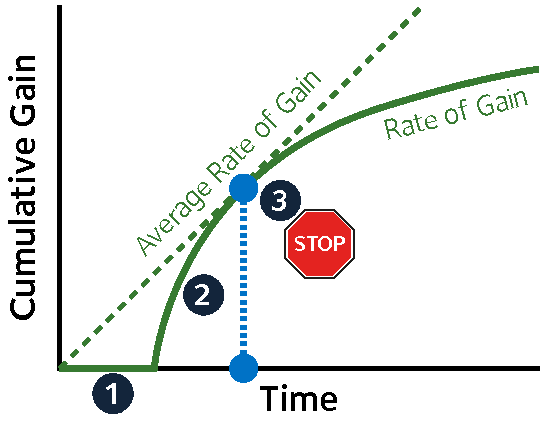
\includegraphics[width=1\textwidth]{figures/ch3-ift_stop.pdf}
    \end{center}
    \vspace*{-4mm}
    \caption[Optimal \gls{acr:ift} stopping heuristic]{The~\gls{acr:ift} stopping heuristic. The searcher should stop when the rate of gain (solid {\color{dmax_green}green} line) no longer outperforms the average rate of gain (dotted {\color{dmax_green}green} line).}
    \label{fig:ift_stopping}
\end{wrapfigure}

The~\gls{acr:mvt} implies that is a forager is within a patch that initially looked promising, yet is yielding a rate of gain less than the \emph{average rate of gain,} he or she should abandon the patch and then move to another one. This phenomenon is often called the \emph{instantaneous intake} theorem~\cite{stephens1986foraging_theory}. In the context of information seeking, this would imply a query reformulation. Conversely however, a forager who has found himself or herself in a patch yielding gain at a rate \emph{greater} than the average rate of gain would be best advised to stay within said patch. This is graphically illustrated in Figure~\ref{fig:ift_stopping}, where the \emph{gain curve} for a forager is highlighted in {\color{dmax_green}green.} In addition, the plot illustrates: \raisebox{-.2\height}{
\includegraphics[height=5mm]{figures/ch2-point1.pdf}} the between patch time, where the forager is not acquiring any gain; \raisebox{-.2\height}{
\includegraphics[height=5mm]{figures/ch2-point2.pdf}} the within patch time, where the forager is examining the~\gls{acr:serp} and associated documents; and \raisebox{-.2\height}{
\includegraphics[height=5mm]{figures/ch2-point3.pdf}} the optimal stopping point, based upon the~\gls{acr:mvt}. Graphically, this is best described as the point at which the tangent to the curve (from the origin) touches the gain curve. From this point onwards, the rate of gain decreases, meaning that the forager receives diminishing returns for the investment in examining content on the current patch.

\begin{figure}[t!]
    \centering
    \resizebox{1\hsize}{!}{
    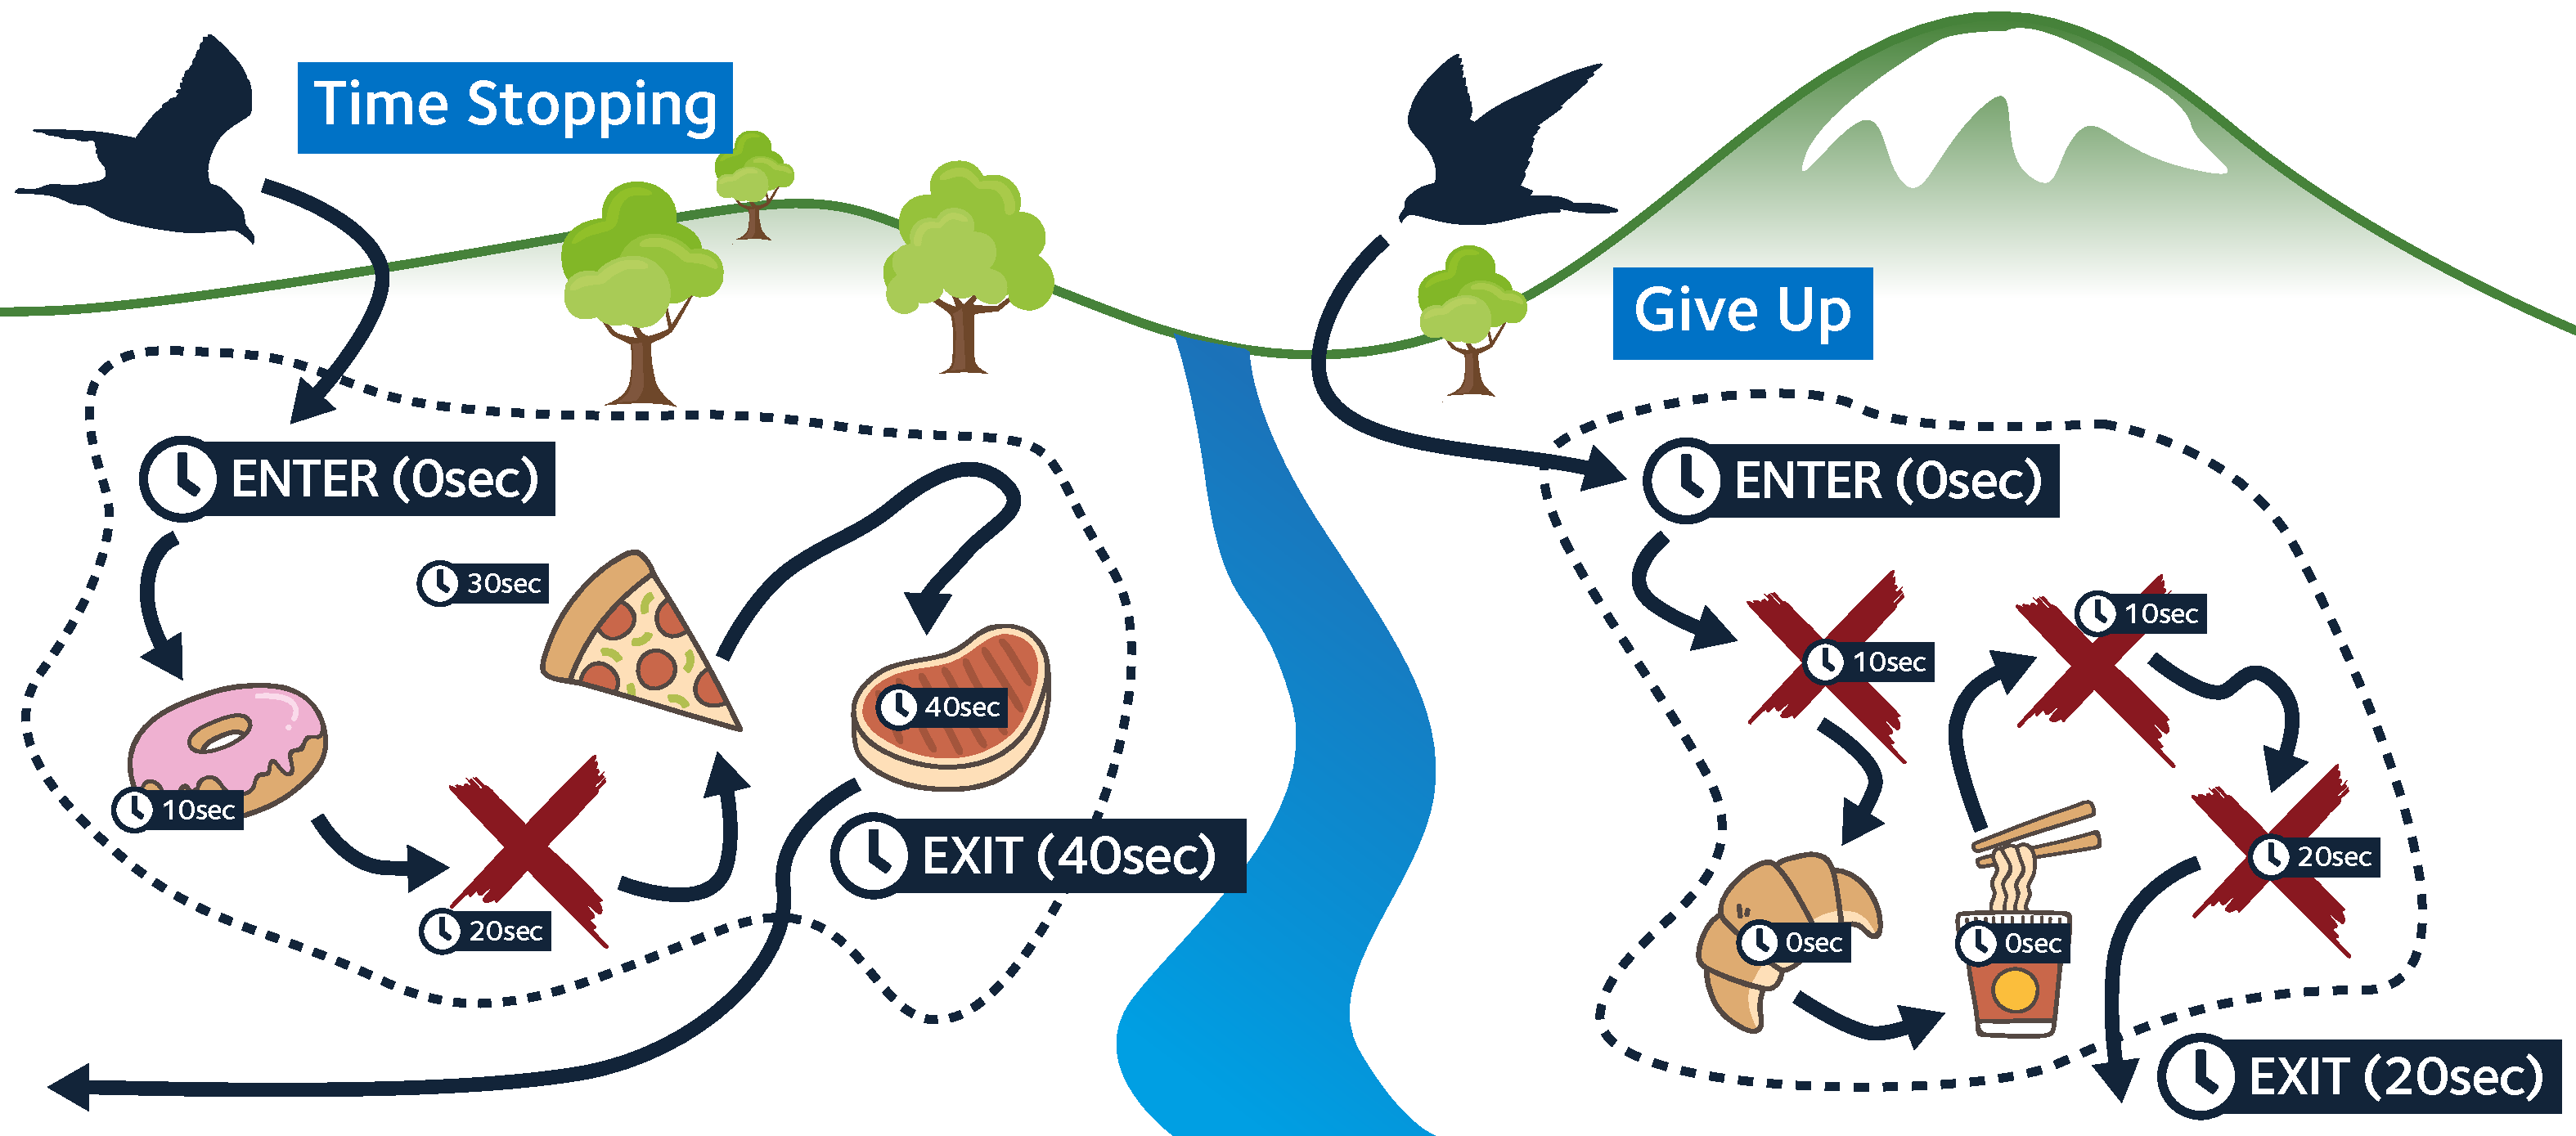
\includegraphics{figures/ch3-gut.pdf}}
    \caption[Time-based stopping heuristics]{Graphical illustrations of the \emph{time stopping heuristic} (left), and the \emph{give up heuristic} (right). On the left, a forager will stop after a time limit has been reached (40 seconds in this example) from the point at which they enter a patch. On the right, a forager will \emph{reset} their timer when they encounter something gainful, but will grow increasingly impatient the poorer the results of their foraging, and eventually stop too (a 20 second limit is shown here).}
    \label{fig:gut}
\end{figure}

Operationalising the instantaneous intake theorem is often difficult to do in practice. How would one measure, for example, the expected rate of gain? Instead, several other stopping heuristics that influence patch leaving have been developed as part of~\gls{acr:oft}~\citep{stephens1986foraging_theory}. These attempt to approximate the instantaneous intake theorem. Such heuristics include, but are not limited to:

\begin{itemize}
    \item{the so-called \blueboxbold{number heuristic}~\citep{gibb1958number_rule}, where a forager would leave a patch after finding $n$ prey;\footnote{This stopping heuristic is analogous to the satisfaction and satiation stopping heuristics, defined by~\cite{cooper1973retrieval_effectiveness} and~\cite{simon1955satiation} respectively.}}
    
    \item{the \blueboxbold{time heuristic}~\citep{charles1972behaviour, krebs1973time_rule}, where a forager stops after spending $x$ seconds within a patch; and}
    
    \item{the \blueboxbold{give up} heuristic~\citep{krebs1974leave_after_rule}, where a forager would stop and leave a patch after $x$ seconds have elapsed since last finding something of use.}
\end{itemize}

The time based stopping heuristics are illustrated in Figure~\ref{fig:gut}. A further study of different \emph{patch types} (i.e. where the density of prey varies) was also undertaken by~\cite{mcnair1982gut_mvt}. They found that across different patch types, different stopping heuristics worked better in different environments -- also demonstrated in works by~\cite{iwasa1981prey_distribution},~\cite{mcnair1982gut_mvt} and~\cite{green1984oft_stopping}. Consequently, a further \blueboxbold{combination heuristic} was devised where in a patch that that is fruitful early on, a satisfaction based heuristic would perform well; otherwise, employing the give up time-based heuristic~\citep{krebs1974leave_after_rule} would work best. This intuitively makes sense: a searcher, when presented with a~\gls{acr:serp} of high quality, would do well to continue to examine it for more content if the initial results are promising. If initial results however are not promising, the searcher should be more sceptical about the results, and be prepared to abandon it if, after examination, relevant content was not forthcoming.

%In other words, a searcher should stop when the marginal gain equals the marginal cost of examining the results.

% \subsection{Other Theoretical Models of Search}\label{sec:stopping_background:theoretical:other}
% It is important to acknowledge that apart from~\gls{acr:ift}, other competing theoretical models of search exist and are being actively developed. The two competing models are~\glsfirst{acr:set}~\citep{azzopardi2011economics} and the~\glsfirst{acr:iprp}~\citep{fuhr2008iprp}. These models have both been shown to be mathematically similar to~\gls{acr:ift} in terms of explaining searcher behaviours -- as shown by~\cite{azzopardi2015theories} -- and as such we limit discussion of these two theoretical models to a brief overview.
%
% As the name suggests,~\gls{acr:set} concerns the modelling of the search process by addressing it as an economics problem, using \emph{production theory}~\citep{varian1987intermediate}. In production theory, a \emph{output} is produced by a firm (goods or services), but requires \emph{input} (capital or labour). The intermediary process employs some form of \emph{technology} to produce the given goods, or to provide the service. In the context of the search process, this maps to the following two inputs:
%
% \begin{itemize}
%     \item{$Q$, the number of \emph{queries} that a searcher will issue; and}
%     \item{$E$, the number of documents that the searcher will \emph{examine} per query.}
% \end{itemize}
%
% Output is considered as the amount of gain that a searcher extracts from the relevant documents that are found. These can be then combined to create \emph{gain functions} (i.e. $g(Q,E)$) and \emph{cost functions} (i.e. $c(Q,E)$). From these, different hypotheses can be generated, as used by~\cite{azzopardi2013query_cost}, and demonstrated in Section~\ref{sec:stopping_background:user_studies:depths}.
%
% The second theoretical model is the~\gls{acr:iprp}. Essentially, the~\gls{acr:iprp} forms an extension to the~\glsfirst{acr:prp}~\citep{robertson1977prp}, but relaxed a number of modelling assumptions made by the~\gls{acr:prp}, namely:
%
% \begin{itemize}
%     \item{the notion of a fixed information need; and}
%     \item{the relevance of a document is independent of previously seen documents.}
% \end{itemize}
%
% While these approximations do offer reasonable assumptions, they have been shown to break down in the past~\citep{gordon1991utility_theory}. The high level, generalisable~\gls{acr:iprp} accounts for different costs and benefits that are associated with particular \emph{situations} and \emph{choices} when ranking a series of documents.

\section{User Studies}\label{sec:stopping_background:user_studies}
While stopping heuristics provide a means for quantitatively characterising and predicting stopping behaviour~\citep{wu2014information_scent}, only a handful of user studies have been undertaken that attempt to understand when enough information is enough~\citep{zach2005enough_is_enough}. As we have already discussed, stopping is an inherently difficult phenomenon to model effectively -- this is because it is instrumented by a series of internal factors to the decision maker's thinking~\citep{nickles1995judgment}. In this section, we detail a number of different user studies that have attempted to provide an explanation for a searcher's stopping behaviour.

\subsection{Understanding Stopping Behaviours}
Two user studies by~\cite{zach2005enough_is_enough} and~\cite{berryman2006defines} have reported on an of stopping behaviours through a series of interviews with subjects. These studies primarily focused on the notion of \emph{why} searchers stopped when they did, both considering subjects seeking information in an academic work environment.

\cite{zach2005enough_is_enough} considered how senior art administrators determined when to stop searching in their daily jobs, and found that they mostly stopped either because they either:

\begin{itemize}
    \item{felt satisfaction with the information that they had obtained during their search;}
    \item{stopped because of time constraints.}
\end{itemize}

The study by~\cite{berryman2006defines} was conducted in a similar vain, where public sector policy workers reported finding it difficult to work out how much information would be enough to satisfy their tasks when initiating them. However, once the structure of what they needed to find has been established, the point at which they felt they should stop became clearer. The findings from this second study provide evidence that the assessments of what constitutes as \emph{enough} can be difficult and complex to deduce. This finding also provides evidence of the development of an underlying mental model of the given information need, and provides justification for the representational stability, propositional stability, and mental list stopping heuristics (as discussed in Section~\ref{sec:stopping_background:heuristics:reasoning}).

A number of user studies have also examined stopping behaviour in relation to the concept of satisfaction or satiation~\citep{simon1955satiation}. As previously discussed in Section~\ref{sec:stopping_background:heuristics:frustration}, this concept suggests that a searcher will cease searching as soon as conditions arise, instead of after they have exhaustively considered all available information~\citep{march1994primer}.

Considering this approach,~\cite{agosto2002satisficing} examined the decision making of young people when searching on the~\gls{acr:www}. In this study, 22 9\textsuperscript{th} and 10\textsuperscript{th} grade students from a U.S. high school demonstrated limitations which affected their decision making, including time constraints that were imposed externally and internally, information overload and other physical constraints. In order to find websites to help in satisfying their information need, the students used reductive approaches to decrease the amount of information presented on the~\gls{acr:www}, and used this to work out when to stop. How students perceived the websites was also largely down to personal preference.

With a completely different set of subjects,~\cite{mansourian2007search} conducted a study where they analysed the stopping behaviours of 37 staff and students from four university biology departments, and classified their stopping behaviours by search depth and search impact. Qualitative results showed that subjects indicated that missing potentially important information in the course of their searching was a matter of concern. The authors reported that the estimations and importance of information missed likely would affect their stopping behaviour. From this, classifications of the perceptions of missing information ranged from \emph{inconsequential} to \emph{disastrous}, and search strategies classified as \emph{perfunctory} to \emph{extensive}, with the information need dictating what category the searcher would have considered appropriate.

A similar study by~\cite{prabha2007enough} considered searchers in a further academic library setting, with one key finding from their study showing that time constraints led to a decrease in the number of documents that searchers examined. Again, the specific information need and the searcher's role in academia affects every stage of their search processes -- which includes affecting what they have found to be enough.

These findings were further demonstrated by~\cite{wu2014information_scent}, who undertook a study where subjects performed a series of different search tasks. Subjects were then interviewed about their query stopping and task stopping behaviours. Results from this study showed that query stopping decisions were taken primarily on the face of search results, queries and search tasks. Task stopping decisions were determined by the subject's overall goal for each task, the content examined -- and their subjective perceptions of the examined content -- and the study constraints imposed upon them, such as time constraints and search interface restrictions. Further empirical evidence to this study was later provided by~\cite{wu2014stopping_query_abandonment}. They reported that some subjects discussed \emph{``forced stopping''} (stopping when no more information could be found), and \emph{``voluntary''} stopping that stemmed from the feeling of securing enough (or a necessary amount of) information.

\cite{wu2014information_scent} also discussed how the \emph{information scent}, defined in Section~\ref{sec:stopping_background:theoretical:ift:patch}, affects the stopping behaviour of a searcher. Constituting part of~\glsfirst{acr:ift} that we discuss in Section~\ref{sec:stopping_background:theoretical:ift}, it is important to note that user studies have been conducted using this model. For example,~\cite{card2001scent_graphs} observed that if a person started with a high information scent web page, he or she would visit more web pages at the site. They also found that as the information scent of web pages declined, there was a tendency for the person to leave the site or return to a previously visited page.~\cite{loumakis2011image_smells} examined scent that was associated with images presented on~\glsplural{acr:serp} impacted with the evaluation behaviour of searchers. They found that when images were added to text snippets, participants reported increased confidence that they could find an answer.

Central to the findings of all of the above studies -- regardless of the group of subjects or contexts in which they found themselves to search in -- is the idea that searchers stop when they are \emph{satisfied.} Even though subjects of these studies were acutely aware of the fact they had not found \emph{all} relevant information to their given information need, they were nevertheless satisfied with what they had found, and subsequently decided to stop. While the results from these studies may be underwhelming in terms of concrete explanations as to why people do stop, they do provide invaluable insights -- and demonstrates just how difficult it is to encapsulate such behaviour. Indeed, factors such as time constrains, a searcher's information seeking ability and other factors all influence the internal stopping rules of a searcher, as was discussed by~\cite{marchionini1995information_seeking}. 

\subsection{Quantifying Stopping Behaviours}
With the above studies examining \emph{why} people decide to stop, a very limited number of studies have attempted to quantify \emph{when} a searcher should stop searching -- somewhat akin to the stopping heuristics defined in Section~\ref{sec:stopping_background:heuristics}.~\cite{toms2009predicting_stopping} studied the actions preceding the endpoints in information, seeking to predict what actions would lead a searcher to stop. The most prevalent patten they observed -- that matches the searcher models outlined in Section~\ref{sec:ir_background:user:models} -- consisted of a searcher:

\vspace{-5mm}
\begin{itemize}
    \item{issuing a query;}
    \item{examining results presented to them on a~\gls{acr:serp}; and}
    \item{viewing a document.}
\end{itemize}
\vspace{-5mm}

Interestingly, the authors observed that searchers appeared to be more engaged in page content and in revisiting and assessing pages that had already been found. They hypothesised that this again may be due to the satiation heuristic, where the searchers would purposefully go back to reassess if what they had found was \emph{enough.}

A further study by~\cite{dostert2009satisficing} examined the stopping behaviours of 23 undergraduate students. Subjects, like in other studies, reported that the primary factor for deciding to stop was their intuition. Again, subjects were time constrained.~\cite{dostert2009satisficing} reasoned that subjects could not adequately articulate this intuition, but hypothesised that they simply felt that given their perception of how much time had elapsed, the number of documents that they had located felt sufficient. The authors however report a number of additional reasons (as shown in Figure~\ref{fig:stopping_respondents}) why subjects decided to stop, with the reasons providing links back to the stopping heuristics defined in Section~\ref{sec:stopping_background:heuristics}.

Indeed, the unarticulated notion of finding \emph{``enough''}~\citep{zach2005enough_is_enough} information links neatly back to the idea of the magnitude threshold stopping heuristic, proposed by~\cite{nickles1995judgment} and detailed in Section~\ref{sec:stopping_background:heuristics:magnitude}. With this heuristic, a searcher would stop once they have accumulated a certain predetermined amount of information. From the results of their study,~\cite{dostert2009satisficing} hypothesised that the threshold was reached once they felt they had correctly identified \emph{half} of the relevant documents available to them. In reality however, the searchers had on average only managed to correctly identify $7.35\%$. In addition to comparisons to the magnitude threshold stopping heuristic,~\cite{dostert2009satisficing} also drew comparisons from their results to the difference threshold stopping heuristic, as outlined in Section~\ref{sec:stopping_background:heuristics:difference}. Recapping, this heuristic considered a searcher's tolerance to not learning anything new -- this is argued by the authors as a reason for respondents citing repetition in the documents found, or a lack of new documents. Lastly, the representational stability stopping heuristic as detailed in Section~\ref{sec:stopping_background:heuristics:representational} was also noted by the authors. With this heuristic concerned with the searcher's underlying mental model of the topic stabilising, the authors noted that evidence for this was shown from subjects responding that a decreasing in relevant documents and an increase in non-relevant documents.

\begin{wrapfigure}[12]{r}{0.45\textwidth}
    \begin{center}
    \vspace*{-10mm}
    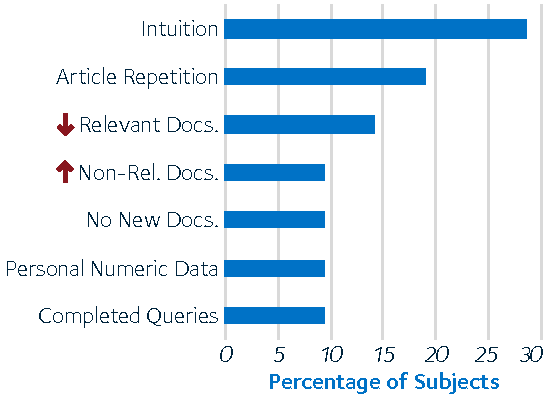
\includegraphics[width=1\textwidth]{figures/ch3-respondents.pdf}
    \end{center}
    \vspace*{-4mm}
    \caption[Responses of a survey by~\cite{dostert2009satisficing}]{Responses of the survey on why subjects stopped by~\cite{dostert2009satisficing}. Like most studies examining stopping behaviour, most subjects stopped because of their \emph{intuition.}}
    \label{fig:stopping_respondents}
\end{wrapfigure}

These stopping heuristics were also investigated by~\cite{browne2004stopping_rules} and~\cite{pitts2004stopping_rules} with systems analysts during the process of information requirements determination. The analysts were tasked to gather a series of requirements until they had acquired enough information to draw diagrams of an online grocery shopping system. It was found by~\cite{browne2004stopping_rules} that more experienced analysts tended to use the mental list and magnitude threshold stopping heuristics, with less experienced analysts employing the difference threshold and representational stability stopping heuristics. In addition to these findings, the authors noted that the applicability of different stopping heuristics resulted in varying degrees of quantity, depth and the quality of information obtained.

\subsection{Considering Search Depths}\label{sec:stopping_background:user_studies:depths}
\begin{wrapfigure}[9]{r}{0.45\textwidth}
    \begin{center}
    \vspace*{-7mm}
    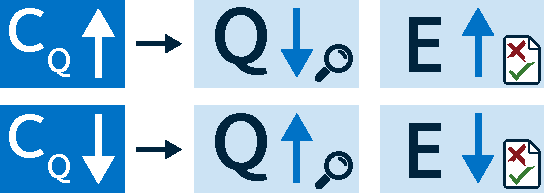
\includegraphics[width=1\textwidth]{figures/ch3-query-cost.pdf}
    \end{center}
    \vspace*{-4mm}
    \caption[The cost-interaction hypothesis]{The \emph{cost-interaction hypothesis}~\citep{azzopardi2011economics}. As the cost of querying increases (\emph{C\textsubscript{Q}}), searchers will issue fewer \textbf{Q}ueries and \textbf{E}xamine more documents per query.}
    \label{fig:query_cost}
\end{wrapfigure}

A number of additional user studies have also considered the so-called \emph{search depth} -- that is, the depth on a list of ranked results that searchers stop clicking (the \emph{click depth}). Studies such as the seminal work by~\cite{cutrell2007eye_tracking} undertook an eye tracking study, and reported that subjects examined the first eight results before deciding to carry out a query reformulation.~\cite{lorigo2008eye_tracking} also examined their subjects' scan paths as they undertook search tasks. On average, subjects scanned only $3.2$ distinct search results per query. This work was supplemented by~\cite{huang2011no_clicks}, where they found that subjects proceeded to issue a new query after inspecting the top four results of the presented~\gls{acr:serp}.

A study by~\cite{azzopardi2013query_cost} also found that the depth to which subjects examined content was affected by the \emph{cost} of entering a query. With a search interface where subjects were required to invest more effort to enter a query, significantly fewer queries were issued, with the results for these queries examined to greater depths. This was in contrast to subjects who used a standard search interface, where more queries were issued, with subjects examining content to shallower depths. These findings comply with the \emph{query-cost hypothesis}~\citep{azzopardi2011economics}, that states that:

\begin{quote}
    \emph{as the cost of querying increases, searchers will pose fewer queries and examine more documents per query.}
\end{quote}

This is illustrated in Figure~\ref{fig:query_cost}. Evidence from this study also demonstrated that the search interface searchers are subjected to impacts upon their stopping decision making.

\section{Chapter Summary}
This chapter has provided an extensive overview of how stopping has been examined in the context of~\gls{acr:iir}. In particular, we have detailed a number of different \emph{stopping heuristics} that have been proposed in the literature. These heuristics are the attempts of researchers to capture a searcher's feeling of what is \emph{``good enough''}~\citep{zach2005enough_is_enough}. We also discussed theoretical models of search, examining in particular~\glsfirst{acr:ift}. This theory provides an explanation as to why and when searchers should stop, and extensive work in the literature based upon~\glsfirst{acr:oft} has also yielded a series of additional stopping heuristics.

We also provided an overview of the literature concerning user studies and searcher stopping behaviours. Many of these studies showed that searchers are simply unable to articulate why they stopped when they did, with internal heuristics causing them to stop when they simply felt satisfied, perhaps complying with the \emph{satisfaction stopping heuristic.} However, these different internal stopping heuristics vary from person to person, with factors such as domain knowledge -- and external factors such as time constraints -- affecting their behaviours~\citep{marchionini1995information_seeking}. As such, this does make stopping behaviours an intrinsically difficult phenomenon to capture and understand effectively.

With the scope and background of this thesis now outlined, we now move towards Part~\ref{part:stopping}. In this following part, we begin to introduce the contributions that this thesis provides, beginning with an updated searcher model. We will also discuss how we operationalised the \emph{stopping heuristics} outlined in this chapter, turning them into a series of programmable \emph{stopping strategies.}

    %!TEX TS-program = xelatex
%!TEX root = ../../maxwell2018thesis.tex

\part[Stopping and IIR Modelling]{In this part of the thesis, we lay out the different stopping strategies that we will consider, as well as demonstrating advancements to user modelling within the IIR process. We also lay out the basic mixed methodology used within this thesis.}{Stopping and IIR Modelling}\label{part:stopping}
    %!TEX TS-program = xelatex
%!TEX root = ../../maxwell2018thesis.tex

\chapter[The Complex Searcher Model and Stopping Strategies]{The Complex Searcher Model\\and Stopping Strategies}\label{chap:csm}
In Part~\ref{part:intro}, we provided a comprehensive overview of the current state-of-the-art of user modelling within the field of~\gls{acr:iir} -- and stopping within search. In this chapter, we present an improvement on the current state-of-the-art, providing an outline of the main conceptual and theoretical contributions of this thesis, which include proposals of:

\vspace*{-2mm}
\begin{itemize}
    \item[\blueboxbold{(i)}]{a more complex and realistic user model -- the~\glsfirst{acr:csm} -- that captures the key interactions that take place during an~\gls{acr:iir} session (Section~\ref{sec:csm:csm}); and}
    \item[\blueboxbold{(ii)}]{an enumeration of a number of \emph{stopping strategies} that we will be evaluating (Section~\ref{sec:csm:stopping}).}
\end{itemize}
\vspace*{-2mm}

These outlines provide the foundations for the subsequent contributory chapters of this thesis that aim to both evaluate the quality of the proposed~\gls{acr:csm}, and the effectiveness of the proposed stopping strategies. Each of the stopping strategies that are proposed in this chapter are operationalised from a number of stopping heuristics defined in the literature, reviewed previously in Chapter~\ref{chap:stopping_background}. To complement the above, we also provide in this chapter \blueboxbold{(iii)} a high level description of the basic methodology we employ in subsequent chapters of this thesis (Section~\ref{sec:csm:methodology}).

\section{The Complex Searcher Model}\label{sec:csm:csm}
The~\glsfirst{acr:csm} is a high level, conceptual model of the search process that captures the key processes and decisions that are taken by a searcher during the information seeking process. Illustrated in Figure~\ref{fig:csm}, the~\gls{acr:csm} is an amalgamation and further development of prior, established models that capture the information seeking process. Discussed previously in Section~\ref{sec:stopping_background:models:conceptual}, prime examples of prior models include the Markov-based approach by~\cite{baskaya2013behavioural_factors}, and the searcher model proposed by~\cite{thomas2014modelling_behaviour}. These models (along with others) are in broad agreement with the general sequence of events that searchers undertake -- from issuing a query to examining documents for relevance. Refer to Figures~\ref{fig:baskaya_model_flow} and~\ref{fig:thomas_model} on pages~\pageref{fig:baskaya_model_flow} and~\pageref{fig:thomas_model} respectively for illustrations of the two aforementioned models.

Given the \emph{baseline models} outlined above and in Section~\ref{sec:stopping_background:models:conceptual}, the~\gls{acr:csm} offers a number of advancements in modelling the information seeking process. In this section, we outline:

\begin{itemize}
    \item{the \emph{flow} of the model, explaining the different steps and decisions that a searcher undertakes (Section~\ref{sec:csm:csm:flow});}
    \item{the different \emph{stopping decision points} of the model (Section~\ref{sec:csm:csm:stopping}); and}
    \item{the \emph{assumptions} that are made as part of the~\gls{acr:csm} (Section~\ref{sec:csm:csm:assumptions}).}
\end{itemize}

We begin however with an overview of the key advancements that the~\gls{acr:csm} provides over existing models of the information seeking process.

\begin{figure}[t!]
    \centering
    \resizebox{1\hsize}{!}{
    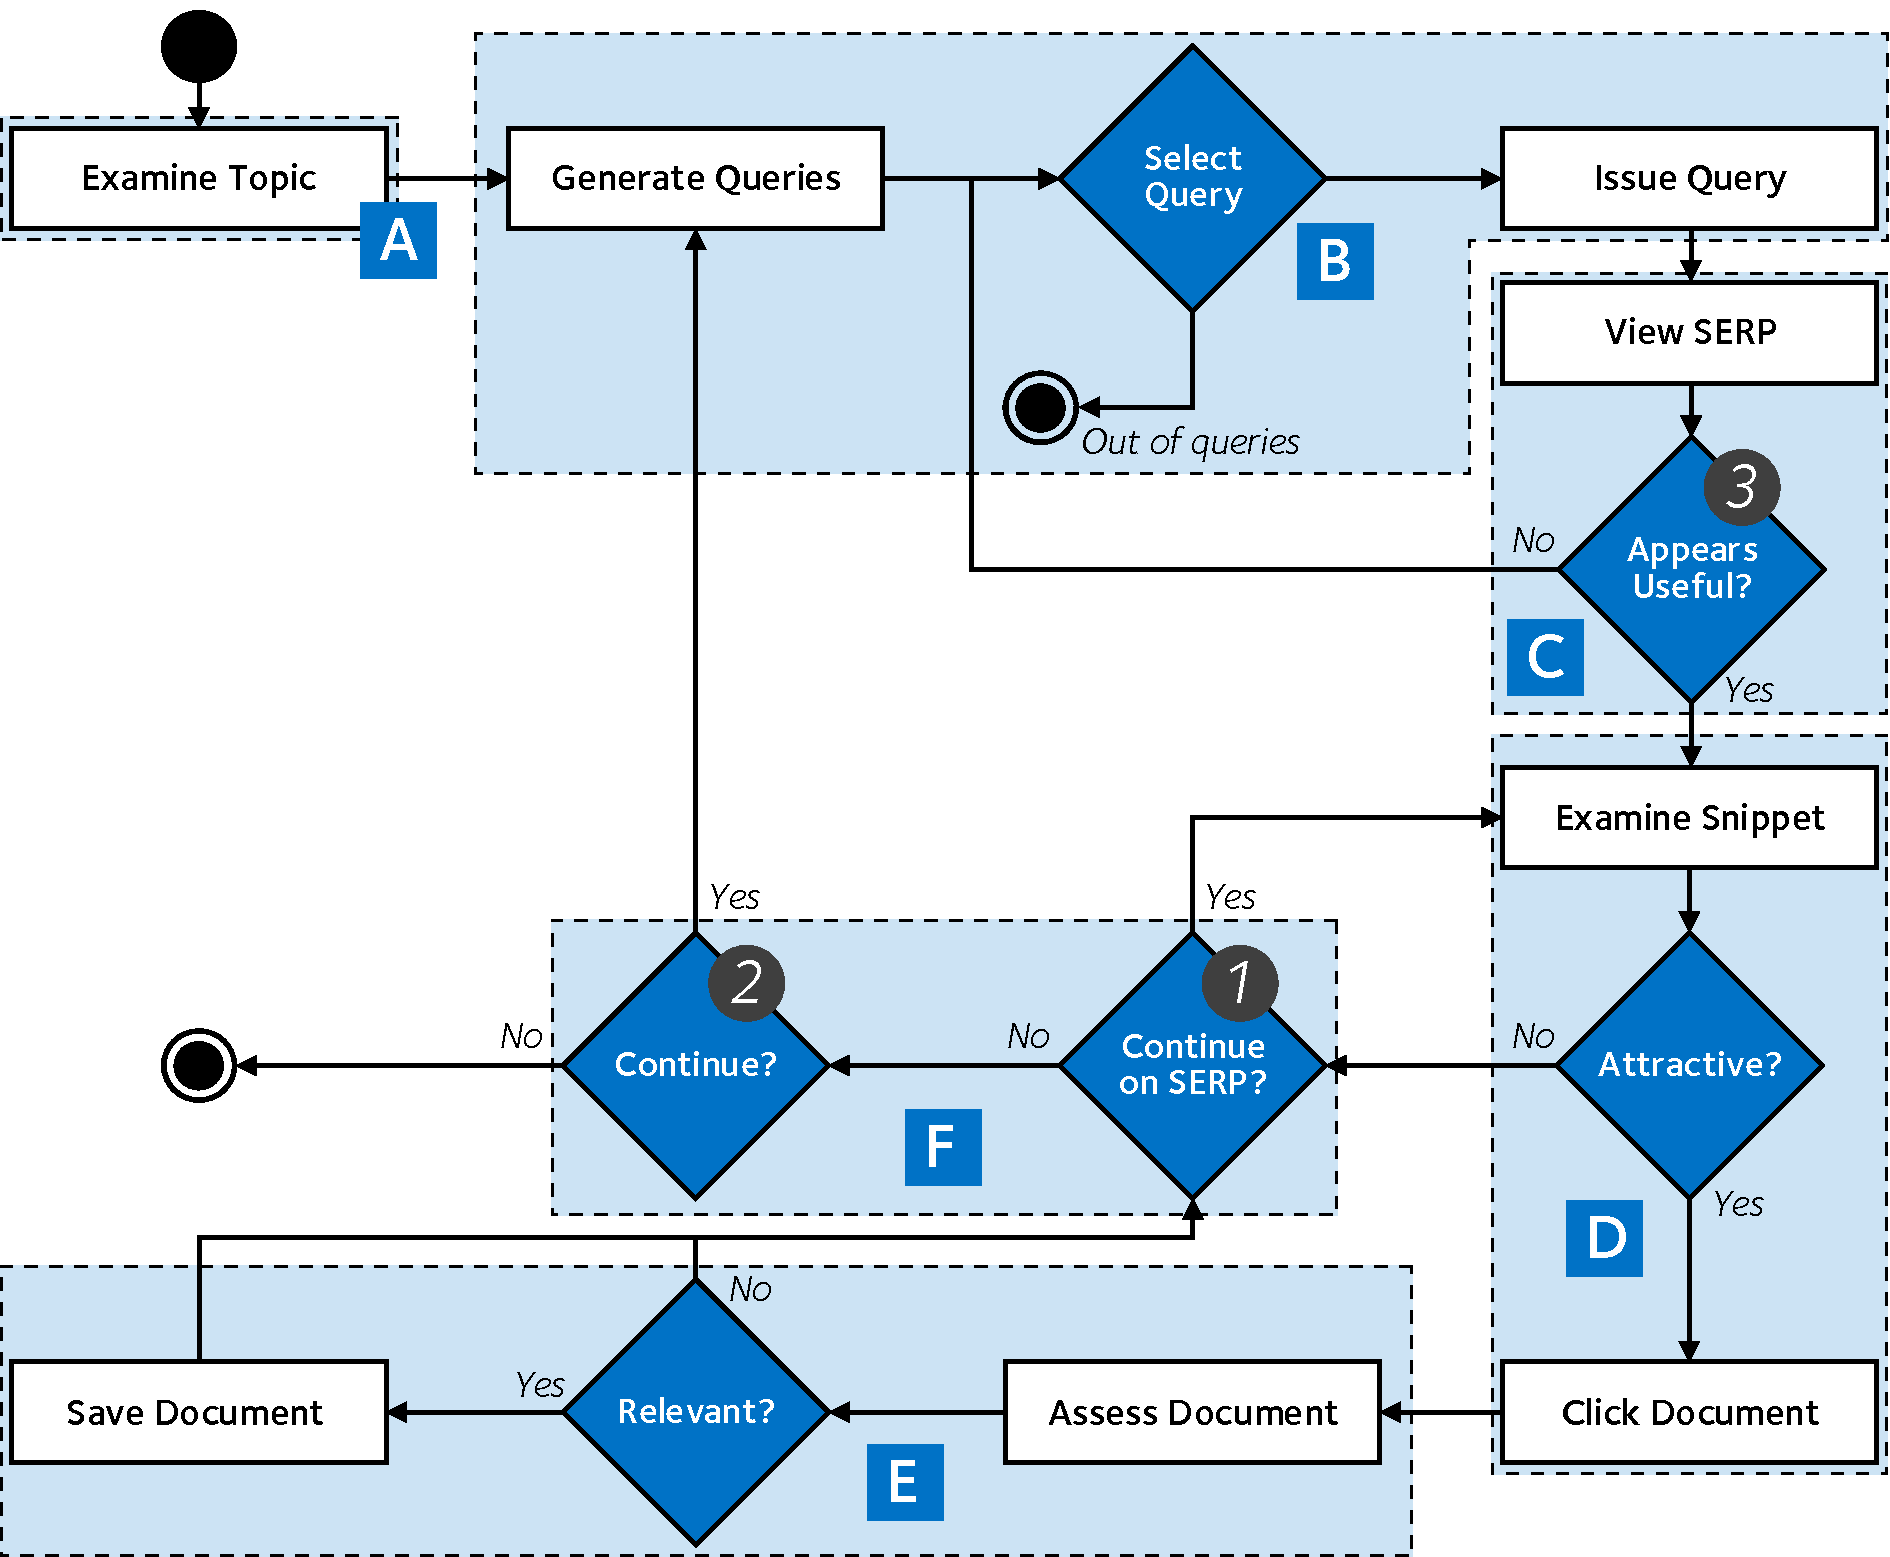
\includegraphics{figures/ch4-csm.pdf}}
    \caption[Flowchart of the~\glsfirst{acr:csm}]{A flowchart of the proposed~\glsfirst{acr:csm}, as used in experimental work discussed later in this thesis. Novel components that the work this thesis provides are highlighted by boxes \blueboxbold{A} and \blueboxbold{B}. The \emph{three} stopping decision points are highlighted with \blueboxbold{1}, \blueboxbold{2} and \blueboxbold{3} (refer to Section~\ref{sec:csm:stopping}). Refer to Section~\ref{sec:csm:csm:flow} for an in-depth explanation of the model.}
    \label{fig:csm}
\end{figure}

\subsection{Model Advancements}\label{sec:csm:csm:advancements}
The~\gls{acr:csm} provides two novel contributions to modelling the information seeking process. The contributions are highlighted as blocks \blueboxbold{A} and \blueboxbold{B} in the~\gls{acr:csm} flowchart provided in Figure~\ref{fig:csm}, and concerns:

\begin{itemize}
    \item[\blueboxbold{A}]{the advancement of modelling the \blueboxbold{querying} aspects of the searcher model; and}
    \item[\blueboxbold{B}]{the introduction of a \blueboxbold{third stopping decision} point concerning the \emph{overall impression} attained of a~\gls{acr:serp} by the searcher.}
\end{itemize}

In the remainder of this section, we discuss these two developments in more detail. While the querying advancements highlighted in block \blueboxbold{A} are novel and intuitive, they are not the core focus of this thesis -- the work detailed in block \blueboxbold{B} is of high relevance, and thus our discussion will be more in depth.

\subsubsection{Modelling the Querying Process}
\begin{publications_box}{Associated Publication}
Work on this advancement of the~\gls{acr:csm} can be found in the following publication.
\vspace*{-2mm}
\begin{itemize}
    \item{\bibentry{maxwell2016agents}}
\end{itemize}
\end{publications_box}

With a search session an inherently interactive process~\citep{ingwersen2005theturn}, a searcher is able to \emph{learn} and develop their mental model of the given information need as they examine information presented to them. As such, during a search task, a searcher may decide to reformulate their query as they obtain a better appreciation of the topic, and are able to formulate a better query, perhaps with descriptive key terms.

As such, the~\gls{acr:csm} provides the mechanism for a searcher subscribing to such a model to update the list of potential queries that could be issued once he or she has finished examining a set of results from the previous~\gls{acr:serp} (labelled as \blueboxbold{Generate Queries} in Figure~\ref{fig:csm}). This is in direct contrast to prior models of search, where queries were selected from a list generated at the start of the search session. This improvement in the modelling process permits a better representation of a searcher's so-called \emph{dynamic information needs}~\citep{borlund2003iir_model}.~\cite{maxwell2016agents} provides an in-depth discussion on this issue.

Once an updated list of queries has been generated, a searcher subscribing to the~\gls{acr:csm} will then make a decision as to \emph{what} query they should issue to the underlying search engine (labelled \blueboxbold{Select Query} in Figure~\ref{fig:csm}). Of course, at this point, a searcher may have exhausted all possible queries, and this is would therefore be a natural stopping point for the searcher. However, as previously discussed, we do not examine this particular component of the~\ref{fig:csm} in any great depth; we do however utilise \emph{querying strategies} that have been previously employed in the literature. Refer to \todo{Section~\ref{}} for more information on these strategies.


\subsubsection{\gls{acr:serp} Level Stopping}
\begin{publications_box}{Associated Publication}
Work on this advancement of the~\gls{acr:csm} can be found in the following publication.
\vspace*{-2mm}
\begin{itemize}
    \item{\bibentry{maxwell2018serp}}
\end{itemize}
\end{publications_box}

As previously mentioned in this section, the second major development, highlighted as block \blueboxbold{B} in Figure~\ref{fig:csm}, is the inclusion of an additional, third stopping decision point. This stopping decision point complements the two established stopping decision points, as discussed in Section~\ref{sec:stopping_background:models:conceptual:simple}.

As outlined by~\cite{maxwell2018serp}, this additional stopping decision point is motivated by the idea of the \emph{information scent} present on a given~\gls{acr:serp}. This was briefly discussed in Sections~\ref{sec:stopping_background:user_studies:understanding} and~\ref{sec:stopping_background:models:theoretical:ift}, and in these sections we highlighted the concept of \emph{proximal cues} providing insights into whether the presented page will yield information that will aid the searcher in satisfying their underlying information need. This has been previously demonstrated in prior studies~\citep{wu2014information_scent, ong2017scent_behaviour, maxwell2017snippets}. By operationalising the notion of information scent as the perceived performance of a given~\gls{acr:serp}, we argue that incorporating this additional activity and stopping decision point allows a searcher to obtain an \emph{impression} of the~\gls{acr:serp} before deciding to \emph{enter} the~\gls{acr:serp} and examine content in detail, or \emph{abandon} the~\gls{acr:serp} and move to the next activity. In other words, when a poor query is issued, the searcher will not expend effort examining content which will have a high probability of not being relevant to their information need. The notion of forming an impression is similar to the summary impressions formed by searchers subscribing to the model defined by~\cite{thomas2014modelling_behaviour}, as detailed in Section~\ref{sec:stopping_background:models:conceptual:simple}. However, in this model, the searcher does not form an overview of the~\gls{acr:serp}, but rather an impression of each summary. This allows him or her to then deduce whether it is enticing enough to examine in more detail.

This is analogous to the well-studied phenomenon of \emph{\gls{acr:serp} abandonment} in which limited interaction occurs with the searcher. This has been typically assumed to provide an indication of the searcher's \emph{dissatisfaction} with the presented results~\citep{dassarma2008serp_abandonment, chuklin2012serp_abandonment}. Thus, we provide, to the best of our knowledge, a model of the search process incorporating a path for a searcher to abandon a~\gls{acr:serp} that appears to be of poor quality (or a \emph{low scent}).

\subsection{Model Flow}\label{sec:csm:csm:flow}
With the underlying assumptions and developments of the~\gls{acr:csm} now outlined, we next provide a high-level description of the various stages of the model. The~\gls{acr:csm} is illustrated as a flowchart in Figure~\ref{fig:csm} on page~\pageref{fig:csm}. Here, the model is described, with an explanation of the different processes involved, and the associated stopping decision points.

When subscribing to the~\gls{acr:csm}, a searcher, once he or she has attained a form of information need, will begin by performing an \blueboxbold{examination of the topic}. This is typically considered to be provided by an experimenter in the form of a \emph{TREC topic}, where a searcher will be provided with a predefined \emph{topic description} of what will constitute as a relevant document (refer to Section~\ref{sec:csm:methodology:collection} for examples). The searcher will then begin to formulate an initial mental model of the topic, identifying key terms and phrases that could be potentially used to translate this information need into a query formulation~\citep{borlund2003iir_model}.

Once a model of the information need has been established, the searcher will then move onto the \blueboxbold{query generation}, \blueboxbold{query selection} and \blueboxbold{query issuance} stages. At this point, the searcher will employ some form of \emph{querying strategy} in order to formulate one or more queries from the underlying model of the information need, and then make a decision, \emph{selecting} one of the candidate queries to take forward and issue to the underlying search engine. As previously discussed, if all candidate queries have been exhausted, the searcher will then stop their search session at this point.

Once a query has been submitted the search engine, the searcher is then presented with the~\gls{acr:serp}. From here, the searcher is able to \blueboxbold{view the~\gls{acr:serp}} -- that is, obtain an \emph{initial impression} from examining the proximal cues presented to him or her. If the~\gls{acr:serp} does not appear to \emph{look good,} or offers a poor information scent, the searcher will abandon the~\gls{acr:serp} and proceed to then issue a further query from the list of candidate queries discussed previously.

If the~\gls{acr:serp} however appears to offer a high information scent, the searcher will then proceed to \blueboxbold{enter the~\gls{acr:serp}}. From here, individual \blueboxbold{snippets will be examined} in detail. As per the assumptions listed above, these are examined in a linear fashion. For each snippet, a judgement is made as to whether the searcher considers it to be sufficiently \blueboxbold{attractive} to click. If deemed sufficiently attractive, the link is clicked, and the searcher is then presented with the \blueboxbold{document} examined in full for an \blueboxbold{assessment}. Once complete, the searcher then makes a further decision with regards to the \blueboxbold{relevancy} of the document to the given information need (or topic, using~\gls{acr:trec} terminology). If deemed relevant, the document is then \blueboxbold{marked} as such, providing a simplistic means for determining what documents have been considered relevant and those that weren't -- refer to Section~\ref{sec:ir_background:user:evaluation:interactive_pr}.

Once the searcher has marked a document as relevant, he or she is returned to the~\gls{acr:serp}. At this point, the searcher must make a decision: \emph{should I continue to examine snippets on this current~\gls{acr:serp}?} This point is also reached by the searcher if he or she judges a snippet to have insufficient attractiveness to pursue further. If the answer is \emph{yes,} the next snippet is examined -- if the answer is \emph{no,} the searcher must then make a further decision. \emph{Given my overall search goals, have I met them? Should I continue my search session?} Search goals will vary between task type -- for ad-hoc retrieval, searchers will often attempt to find a predetermined number of relevant documents before a time limit expires. If the criteria have or criterion has not been met, the searcher will continue his or her search session by jumping back to the near start of the process, and undertake \blueboxbold{query generation} once more. If the stopping criteria have or criterion has been met, then the searcher will then abandon the search session, hopefully satisfied with what he or she has found.

Note that at each process -- whether it be issuing a query or examining a document for relevance -- a searcher will pay some form of \blueboxbold{cost} for the effort that they need to expend performing the aforementioned activity. All of the different components of the~\gls{acr:csm} -- whether they are activities or decision points -- can be instantiated in a number of different ways. For example, stopping strategies that we discuss below in Section~\ref{sec:csm:stopping} can be used to instantiate the different stopping decision points within the model. \todo{What about other bits?}

\subsection{Stopping Decision Points}\label{sec:csm:csm:stopping}
Of central focus to the work in this thesis are the \emph{stopping decision points} of the~\gls{acr:csm}. As previously discussed, the~\gls{acr:csm} contains an additional, third stopping decision point. This is in combination with the two established stopping decision points, as previously highlighted in Section~\ref{sec:stopping_background:models:conceptual:simple} on page~\pageref{sec:stopping_background:models:conceptual:simple}.

The three stopping decision points that the~\gls{acr:csm} considers are listed below. While these are explained in Section~\ref{sec:csm:csm:flow}, it is nevertheless good practice to enumerate them.

\begin{itemize}
    
    \item{\blueboxbold{\gls{acr:serp} Level Stopping} considers the point at which a searcher can abandon a~\gls{acr:serp} after attaining an \emph{initial impression} of the presented~\gls{acr:serp}, thus saving a searcher from examining summaries in depth if the~\gls{acr:serp} appears to be of poor quality.}
    
    \item{\blueboxbold{Snippet Level Stopping} As previously mentioned, this is sometimes labelled as \emph{query level stopping} in the literature. We name this decision point snippet level stopping to remove any ambiguity between~\gls{acr:serp} level stopping and this point. Snippet level stopping considers the depth to which a searcher will traverse a list of results, before deciding to stop their examination.}
    
    \item{\blueboxbold{Session Level Stopping} Finally, session level stopping concerns the notion of when a searcher will decide to terminate their search session altogether. This could be constrained by time limits, or some predetermined notion of how many relevant items they have found.}
    
\end{itemize}

Figure~\ref{fig:csm} on page~\pageref{fig:csm} also provides a visual illustration of the stopping decision points within the wider~\gls{acr:csm} flowchart. Decision points \blueboxbold{1}, \blueboxbold{2} and \blueboxbold{3} represent snippet level stopping, session level stopping and~\gls{acr:serp} level stopping respectively.

How these stopping decision points are operationalised is dependent upon a variety of different factors. For example, the task type is highly likely to influence the overall session stopping strategy that is employed. The literature, as overviewed in Section~\ref{sec:stopping_background:heuristics} provides a number of heuristics to potentially operationalise stopping. These are primarily geared towards the concept of snippet level stopping.

\subsection{Clarifications and Assumptions}\label{sec:csm:csm:assumptions}
As with any model of a real-world phenomenon, the~\gls{acr:csm} also makes a number of key assumptions. Along with clarifications of the model, we list and detail these assumptions below.

\noindent
\blueboxbold{Considering Ad-Hoc Retrieval} The~\gls{acr:csm} considers \emph{ad-hoc retrieval,} a type of search task previously discussed earlier in Section~\ref{sec:ir_background:basics:cranfield:trec}.\footnote{This clarification is included at the request of Distinguished Professor Nicholas Belkin (Rutgers University, NJ, USA), who discussed that the task type the~\gls{acr:csm} models should be clearly defined. This was done at the first \emph{ACM CHIIR} Doctoral Consortium in Chapel Hill, NC, USA -- refer to~\cite{maxwell2016dc} for the associated publication.} Of course, many other different types of search task exist, such as, for example, navigational and patent searching. Ad-hoc retrieval is foundational to many areas of~\gls{acr:ir}\footnote{Referring to \emph{Microsoft} Senior Applied Scientist Peter Bailey's \emph{SIGIR} paper writing tips (available at~\url{https://www.microsoft.com/en-us/research/people/pbailey/} -- last accessed May 1\textsuperscript{st}, 2018), \emph{``there is more to life than ad-hoc''} (tip 10). We agree with this statement, but also argue in the main narrative that the similarities between ad-hoc and other search tasks are similar in nature, making it a sensible choice to consider.} -- but the similarities between ad-hoc and other types of search task provide motivation for selecting such a task to model.

Take, for example, a navigational task. A searcher, wishing to find the electronic commerce site \emph{Amazon}, may issue a query to a commercial web search engine. The query, \texttt{amazon}, yields a series of results presented to him or her on a~\gls{acr:serp}. Typically, if the intent is correctly understood by the search engine, the first result in the verticals links the searcher to Amazon, satisfying his or her information need. This process is largely the same of the~\gls{acr:csm}, as illustrated in Figure~\ref{fig:csm}. Unlike the~\gls{acr:csm} however, the searcher will not complete later stages of the model, such as marking the identified document as relevant -- the searcher will simply abandon the search session.

The argument for using ad-hoc retrieval as the underpinning of the~\gls{acr:csm} is therefore simple. By modelling ad-hoc retrieval, this essentially guarantees that the entire search process -- from query formulation to identifying relevant documents -- is repeated a number of times. As we are modelling the search process in its entirety -- not individual components in isolation -- this makes ad-hoc retrieval a sensible choice.

\noindent
\blueboxbold{Choosing a Search Engine} A searcher, when subscribing to the~\gls{acr:csm}, is assumed to have already undertaken the necessary steps in selecting the search engine most likely to satisfy his or her information need. This is important to clarify, as certain models of information seeking proposed in the literature -- such as the model proposed by~\cite{thomas2014modelling_behaviour} -- include the notion of selecting a search engine within the wider information seeking model. Of course, this is an important step -- selecting a patent search engine\footnote{As opposed to general purpose, commercial web search engines such as \emph{Google} or \emph{Bing,} agencies such as the European Patent Office provide bespoke patent search engines -- refer to \url{https://worldwide.espacenet.com/} for an example (last accessed May 1\textsuperscript{st}, 2018).} for a patent search task would be a prudent choice. We however consider this step superfluous to the requirements of the~\gls{acr:csm} -- the model purely considers the interactions between the user and the search engine, not decisions made before or after.

\noindent
\blueboxbold{Bad and Good~\gls{acr:serp} Abandonment} When considering whether the~\gls{acr:serp} should be abandoned (via the new stopping decision point, summarised in Section~\ref{sec:csm:csm:stopping}), we assume that this is under the pretence of \blueboxbold{bad abandonment} (i.e. a dissatisfaction of the presented results). This is in contrast to the notion of \emph{good abandonment}~\citep{khabsa2016good_abandonment}, which we do not consider in the presented~\gls{acr:csm}. However, future refinement of the model may lead to the ability for the~\gls{acr:csm} to discern between the two -- refer to Figure~\ref{fig:csm_bad_good} for a potential solution to this issue. Indeed, this may be more applicable in future research -- good abandonment is typically prevalent in contemporary~\gls{acr:ir} research (especially on small-screen devices such as smartphones). Furthermore, with the addition of contemporary~\gls{acr:serp} components such as the information card~\citep{bota2016information_cards}, certain information needs can be satisfied by examining the~\gls{acr:serp} without needing to click on any results.

\begin{figure}[t!]
    \centering
    \resizebox{1\hsize}{!}{
    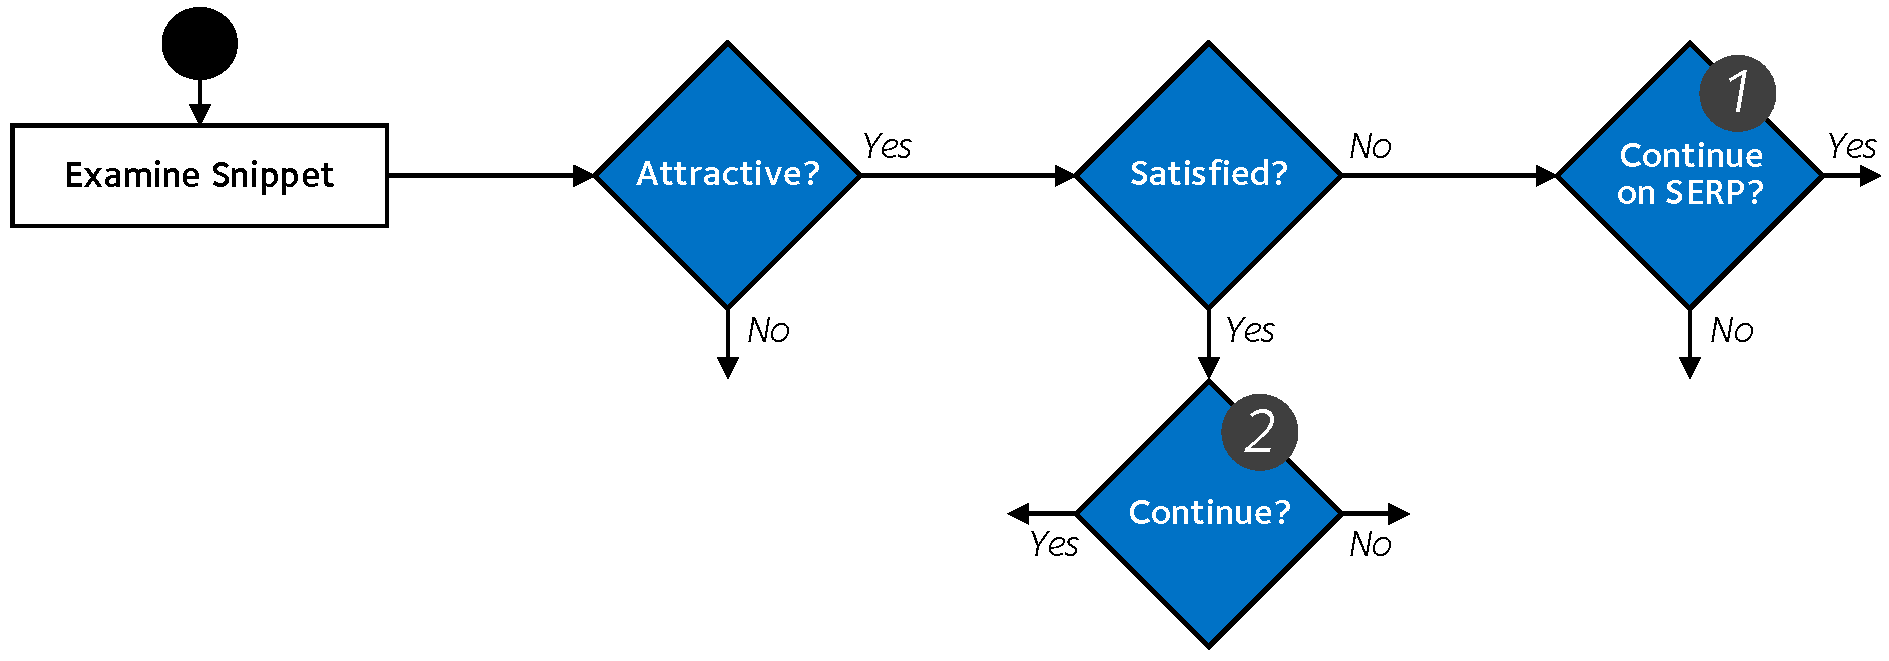
\includegraphics{figures/ch4-good.pdf}}
    \caption[Flowchart considering good abandonment]{A potential solution to also considering good abandonment. After examining a snippet for attractiveness, an additional decision point could allow a searcher to determine that examining the snippet itself satisfies their information need, and thus provide a means by which the searcher could then stop examining results, or stop their search session altogether.}
    \label{fig:csm_bad_good}
\end{figure}

\noindent
\blueboxbold{Simple~\glsplural{acr:serp}} When considering the~\gls{acr:serp} presented to a searcher as a whole, we make three simplifying assumptions within the~\gls{acr:csm}. These are listed and detailed below.

\begin{itemize}
    \item{\blueboxbold{Ten Blue Links} Under the~\gls{acr:csm}, a~\gls{acr:serp} will consist only of one set of \emph{verticals,} i.e. the traditional \emph{ten blue links} that are still present in contemporary~\glsplural{acr:serp}. Of course, we acknowledge that additional components are present in contemporary~\glsplural{acr:serp}, such as multimedia content in federated search~\citep{chen2012federated_search_click_model}.}
    \item{\blueboxbold{Linear Examination Order} Once a searcher has decided to examine a~\gls{acr:serp} in detail, the result summaries presented to the searcher will be examined in the order in which they appear. There is evidence to suggest that real-world searchers examine results from top to bottom, as demonstrated by~\cite{joachims2002click_model} and~\cite{joachims2005click_model}, for example. Click models, such as the \emph{cascade model}~\citep{craswell2008click_models}, have been developed that employ this assumption. Such approaches are subject to \emph{position bias,} where the searcher trusts the results of the retrieval algorithm, assuming that the first result presented in the verticals is the most relevant to their information need.}
    \item{\blueboxbold{No Pagination} The~\gls{acr:csm} also assumes that the~\gls{acr:serp} presented to a searcher is of a single page, and no pagination of results exists. This does simplify the modelling process somewhat, with pagination not considered in prior information seeking models that consider the search session as a whole.}
\end{itemize}

\subsection{Stochastic and Deterministic}
\begin{publications_box}{Associated Publication}
Work discussing the notion of incorporating state and agency into the~\gls{acr:csm} can be found in the following publication.
\vspace*{-2mm}
\begin{itemize}
    \item{\bibentry{maxwell2016agents}}
\end{itemize}
\end{publications_box}

In this section, should I explain the difference between stochastic models of search, and deterministic models of search?
So, in a previous section, we detailed different approaches to simulation.

Stochastic considers a `roll of the dice' to determine whether a searcher will click on a link, for example $P(C)$. And that can be drilled down even more, to consider probability of a click given that it is relevant to some gold standard $P(C|R)$.

Other alternative is to instantiate the model using deterministic components.
So that the searcher is able to deduce, without grounding, what is relevant and not. Dependent upon various components like language models, and is much more complex. This is more in tune with attempting to model the cognitive functions going on inside someone's brain, and is not really the focus of this thesis.

However, we have explored this in detail. In~\cite{maxwell2016agents}, we looked at the notion of developing intelligent search agents with the~\gls{acr:csm}. (Short explanation of paper).

These are dependent upon the state of a user. We argue that even a simple implementation of the CSM itself has some form of state, because it needs to remember things like: what documents it has clicked on, what documents it has marked, and so forth. It needs to keep track of queries it has issued, so it does not issue duplicates. Basic things. In this agency paper, we took it further, so the searcher was able to `learn' and make informed decisions (i.e. training a language model) at each iteration of the search process.

So... in this thesis, we consider only stochastic models of search, where the simulations are grounded with some prior probabilities extracted from interaction data. The approach is discussed more in Section~\ref{sec:csm:methodology}.


\section{Operationalised Stopping Strategies}\label{sec:csm:stopping}
In Section~\ref{sec:stopping_background:heuristics}, we discussed a number of different \emph{stopping heuristics} that have been previously defined in the literature. A majority of these heuristics were derived from the concept of \emph{satiation}~\citep{simon1955satiation} -- that is, the searcher abandons their search when they feel satisfied with what they have found. These heuristics were conceptual in nature, being derived from a number of underlying theories and assumptions.

In this section, we take a number of these stopping heuristics forward to produce a number of different~\glsplural{glos:stopping_strategy}. These strategies are operationalised versions of the corresponding heuristics, which mean we can subsequently implement and test them. The stopping strategies are enumerated, and split into five main categories, as listed below:

\begin{itemize}
    \item{a baseline, \blueboxbold{fixed depth} stopping strategy;}
    \item{a stopping strategy based upon the \blueboxbold{frustration} stopping heuristic;}
    \item{\blueboxbold{satisfaction} based stopping strategies;}
    \item{stopping strategies based upon the \blueboxbold{difference} threshold stopping heuristic;}
    \item{several stopping strategies based upon~\blueboxbold{\gls{acr:ift}}; and}
    \item{two stopping strategies based upon established~\gls{acr:ir} evaluation measures.}
\end{itemize}

Although each of these stopping strategies could in theory be applied to any of the three stopping decision points summarised in Section~\ref{sec:csm:csm:stopping}, we consider them only from a snippet level in this thesis. This does not mean to say we do not explore the additional two stopping decision points -- Chapter~\ref{chap:serp} explores the~\gls{acr:serp} level stopping decision point, and Chapter~\ref{chap:diversity} considers the session level stopping decision point.

In addition to this, not all stopping heuristics outlined in Section~\ref{sec:stopping_background:heuristics} are considered. This is because several of the stopping heuristics are not trivial to implement, and would require considerable effort to model effectively. Furthermore, a number of these heuristics do not necessarily comply with the search task we will be simulating -- the mental list heuristic may not be directly applicable to ad-hoc retrieval, for example.

\todo{The following stopping strategies have been catalogued in Section~\ref{sec:stopping_background:heuristics}. It should be noted that we have not selected rules which are based upon satisfaction or satiation because the task we are investigating is ad-hoc topic retrieval, where the goal is to find as many relevant documents as possible in a given period of time. The satisfaction/satiation rules therefore do not seem particularly applicable in this context. Furthermore, rules such as the mental list rule seem to be more topic specific, requiring a searcher to know in advance all the criteria that they need to check off in their head \emph{a priori}. However, these criteria are largely unknown in ad-hoc circumstances.}

\noindent\blueboxbold{A Note on Usefulness} In this section, we refer to the concept of a result summary being \emph{useful} and \emph{unhelpful}. By this, we mean that a summary appears to be of use for a searcher to satisfy his or her information need. In the context of simulation, this notion of relevance does not necessarily correspond to the judgement made in a gold standard that is being compared to: the notion of usefulness in this context represents the decisions that are taken by a searcher as to what constitutes a useful or unhelpful document/result summary.

\begin{publications_box}{Associated Publications}
A number of the stopping strategies listed below have been previously defined in the following publications.
\vspace*{-2mm}
\begin{itemize}
    \item{\bibentry{maxwell2015initial_stopping}}
    \item{\bibentry{maxwell2015stopping_strategies}}
\end{itemize}
\end{publications_box}

\subsection{Fixed Depth}
The fixed depth stopping strategy is based upon an assumption held across many of the models and measures that are widely used throughout the~\gls{acr:ir} community. This assumption is that a searcher, when examining a list of ranked results for their query, will browse to a \emph{fixed depth} before stopping -- the roots of which can be traced back to the Cranfield Paradigm as discussed in Section~\ref{chap:intro}. Examples of use include the basic stopping model encoded within~\gls{acr:patk}. The assumption is also widely used in the simulation of interaction. For example,~\cite{azzopardi2011economics} conducted a large-scale simulated analysis, where simulated users examined content to depths ranging from $5$ to $1,000$ ($1,000$ is typically assumed in TREC style experimentation, where a single query is issued). Given the wide use of this fixed depth approach in historical and contemporary~\gls{acr:ir} research, we consider this stopping strategy as the baseline approach to which we will be comparing the more advanced, \emph{adaptive} stopping strategies.

\begin{itemize}
    
    \item[]{\blueboxbold{SS1}} Using this stopping strategy, a searcher will stop once they have observed $x_1$ result summaries (i.e. \blueboxbold{SS1} @ $x_1$), regardless of their relevance to the given topic.
    
\end{itemize}

\begin{figure}[t!]
    \centering
    \resizebox{1\hsize}{!}{
    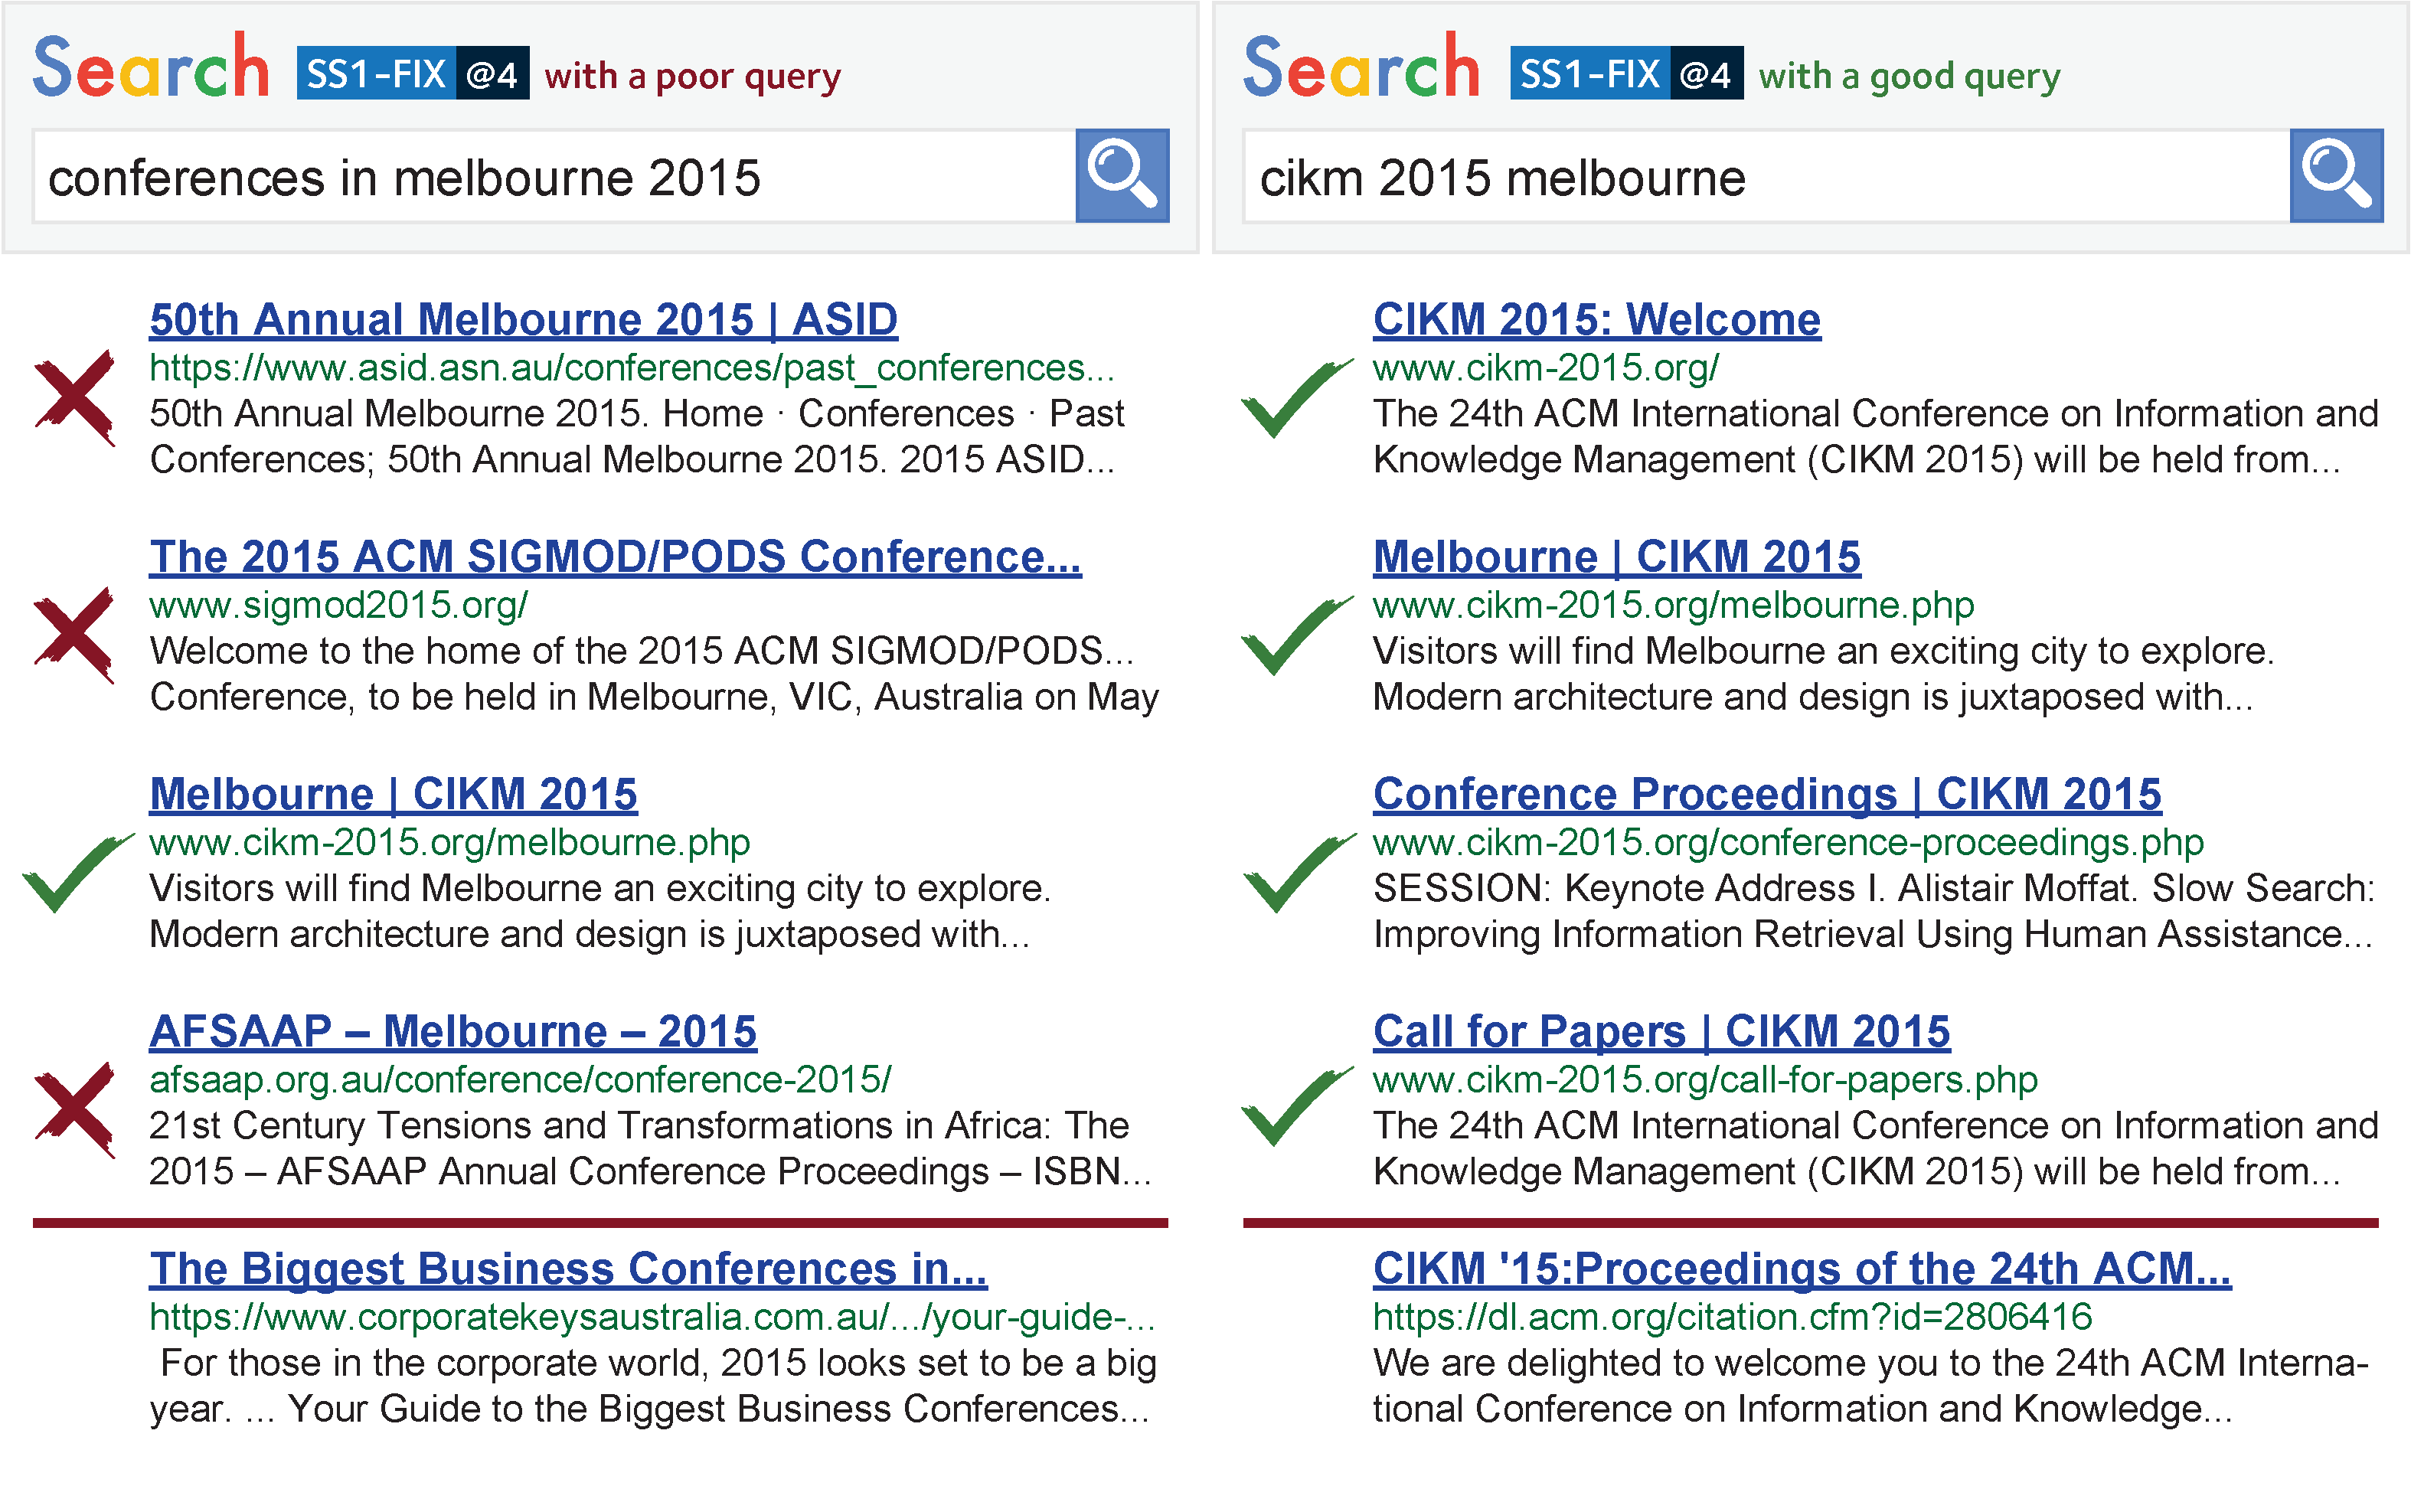
\includegraphics{figures/ch4-ss1.pdf}}
    \caption[Examples of the fixed depth stopping strategy, \blueboxbold{SS1}]{An example of the fixed depth stopping strategy, stylised in this thesis as \blueboxbold{SS1}. Here, a searcher has an information need for the conference \emph{CIKM 2015} in Melbourne, Australia. The left example shows the top five results for poor performing query query, with few useful results (denoted by {\color{dmax_red}crosses}); conversely, the right shows results for a query performing well, with many useful results (denoted by {\color{dmax_green}ticks}). With \blueboxbold{SS1} @4, the searcher will stop at a depth of 4, regardless of the usefulness of the content provided.}
    \label{fig:ss1}
\end{figure}

Given the description of the stopping strategy above, we note that the fixed depth approach is na\"{i}ve in the sense that documents up to rank $x_1$ are useful to the searcher's given information need. On average, such a rule does make sense, but when individual result lists are considered, the approach would not be considered to be a sensible strategy to follow.

Despite the na\"{i}evty of the approach, the other main drawback of such an approach is exposed when a searcher complying with such a strategy issues a poor performing query. This is demonstrated in Figure~\ref{fig:ss1}, with two~\glsplural{acr:serp} presented side by side. Given a searcher's desire to find pages that provide information regarding \emph{CIKM 2015}\footnote{CIKM 2015 was a conference held in Melbourne, Australia, in October 2015. The paper that initially proposed many of these stopping strategies~\cite{maxwell2015stopping_strategies} was indeed presented at this conference.}, two queries are issued: the query on the left yielding poorer results than the query on the right, as denoted by the ticks and crosses, for useful and unhelpful result summaries, respectively. With \blueboxbold{SS1} @4 set, four result summaries are always examined before stopping, regardless of their perceived usefulness. As a result of this, na\"{i}vely examining four documents for the query on the left is by and large a waste of the searcher's time.

\subsubsection{Considering Searcher Frustration and Satisfaction}
In this section, we propose three further stopping strategies, based upon a searcher's tolerance to non-relevance (frustration) and a simple goal-based strategy (satisfaction).

\subsubsection{Searcher Frustration}
he second category of stopping strategies that we propose in this thesis are those that consider a searcher's \emph{tolerance to non-relevance}. Given a set of result summaries presented on a~\gls{acr:serp}, how many would a searcher be prepared to judge to be of no use before they become frustrated, and subsequently abandon their query?

As detailed in Section~\ref{sec:stopping_background:heuristics}, a number of researchers have proposed stopping heuristics that consider non-usefulness (or \emph{non-relevance}, as defined in the literature). The rule intrinsically makes sense for exhaustive searches~\cite{kraft1979stopping_rules}. As an example, when tasked to find as many documents as possible related to different species of animals that are endangered, becoming disgusted with the presented~\gls{acr:serp} when a lack of new species are shown would be a suitable point at which to break and reformulate a new query, or abandon the search session altogether.

From the heuristics defined by~\citealt{cooper1973retrieval_effectiveness_ii} and~\citealt{kraft1979stopping_rules}, we propose two variants of the disgust rules, \blueboxbold{SS2} and \blueboxbold{SS3}.

\begin{itemize}
    
    \item[]{\blueboxbold{SS2}} Under this stopping strategy, the searcher will stop once they have observed $x_2$ unhelpful result summaries. If a result summary has been previously seen in the search session and was considered non-relevant, it is included in the count.
    
    \item[]{\blueboxbold{SS3}} Similar to the stopping strategy defined above above, a searcher employing this stopping strategy will stop once they have observed $x_3$ unhelpful result summaries \emph{in a row (contiguously)}. Previously observed unhelpful result summaries within the search session are included in the count.
    
\end{itemize}

\begin{figure}[t!]
    \centering
    \resizebox{1\hsize}{!}{
    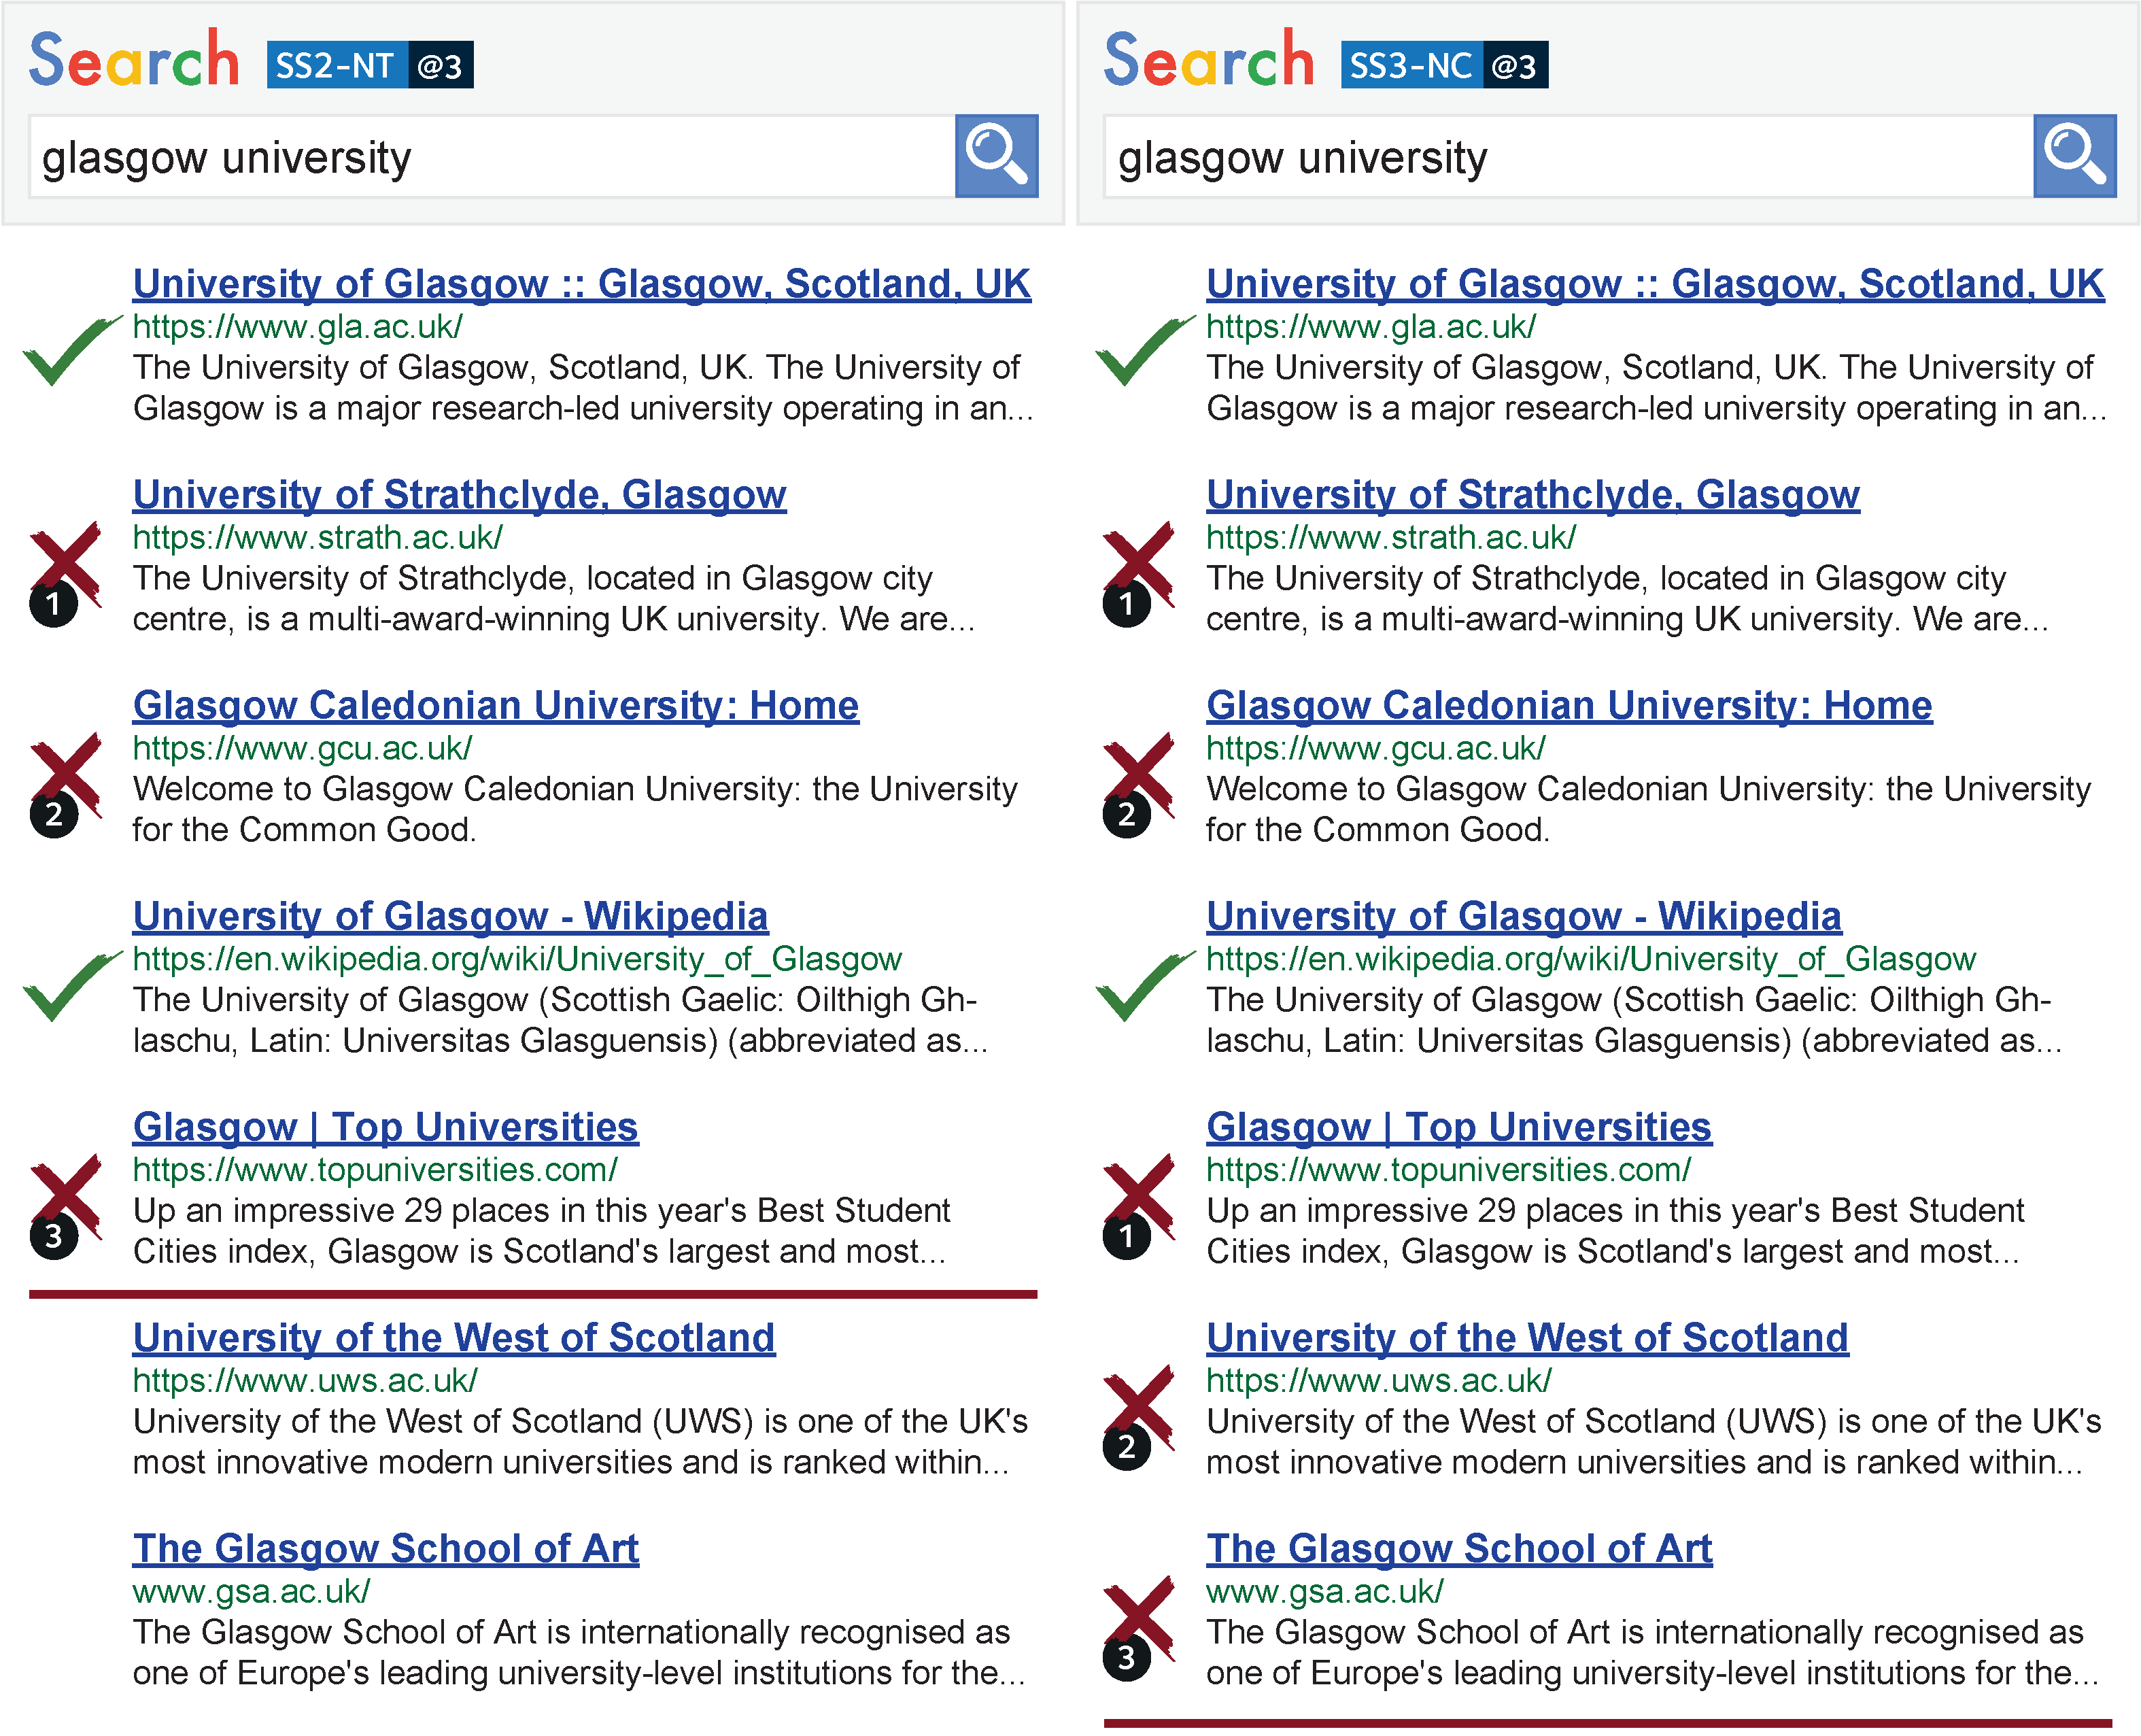
\includegraphics{figures/ch4-ss23.pdf}}
    \caption[Examples of frustration rules \blueboxbold{SS2} and \blueboxbold{SS3}]{An example of the two frustration rules, \blueboxbold{SS2} (left) and \blueboxbold{SS3} (right), both using a parameter of 3 unhelpful result summaries, and under the same query and results. Given that \blueboxbold{SS2} considers the \textbf{total} number of result summaries judged to be unhelpful, a searcher employing this stopping strategy would stop at rank 5 in the example above. Considering a set of contiguous unhelpful summaries, a searcher using \blueboxbold{SS3} would stop at rank 7.}
    \label{fig:ss23}
\end{figure}

As mentioned previously, these two stopping strategies are the first that we enumerate where a searcher would begin to \emph{adapt} their interactions with a ranked list of results, depending upon the performance of the underlying query that was issued. As such, this behaviour inherently makes these stopping strategies more realistic~\cite{moffat2013users_versus_models}. Figure~\ref{fig:ss23} illustrates this adaption in action, with the same query and associated results. On the left of the figure is an illustration of when a searcher employing \blueboxbold{SS2} would stop, and on the right, an example of \blueboxbold{SS3}. We use $x_2 = x_3 = 3$. Under \blueboxbold{SS2}, a searcher would stop at rank 5, while a searcher would stop at rank 7 when employing \blueboxbold{SS3}.

\cite{cooper1973retrieval_effectiveness_ii} highlights the above as one way of operationalising such a stopping strategy: by providing a pre-determined number of documents to stop at. The other approach, which we do not consider in this thesis, would be to allow a searcher to find a series of documents, then go back and count. Such an approach seems unnatural, with the former approach simulating a form of goal-based task. By varying the number of non-relevant documents to stop at, one will be able to attain a better understanding of how performance and other behaviours differ.

\subsubsection{Goal/Satisfaction Based}
Analogous to the frustration rule are the satiation-based stopping heuristics. Here, rather than focus on the frustration or disgust that a searcher might experience when confronted with unhelpful result summaries, satisfaction based rules -- explained in Section~\ref{sec:stopping_background:heuristics:judgement:satisfaction_frustration} -- consider a searcher encountering a number of \emph{useful} result summaries (or documents) before deciding to stop.

\begin{itemize}
    \item[\blueboxbold{SS4}] A searcher using this stopping strategy will stop examining content after encountering $x_4$ useful result summaries.
\end{itemize}

While demonstrated above in the context of snippet level stopping, such a strategy, depending upon the search task, may not be particularly useful when operationalised at this stopping decision point. For example, consider the scenario where a searcher issues a poor query, yielding next to no summaries deemed to be worthy of further examination. In this scenario, a searcher fully complying with \blueboxbold{SS4} may struggle to find enough documents to reach their goal, and this will waste time examining poor results. Such a stopping strategy may be better suited to an overall search goal (i.e. a session level stopping strategy), and deploying a more suitable stopping strategy for snippet level stopping decisions.


\subsubsection{Combining Frustration and Satisfaction}
Considering satisfaction and frustration based stopping heuristics,~\citealt{kraft1979stopping_rules} also proposed a \emph{combination heuristic} that combined both approaches together. Employing this heuristic, a searcher would stop when they became frustrated, or were satisfied by what they saw -- whatever comes first. As such, we can convert this into a stopping strategy, as described below.

\begin{itemize}
    \item[\blueboxbold{SS5}] A searcher utilising this stopping strategy will employ \blueboxbold{SS2} and \blueboxbold{SS4} to determine when to stop, ceasing their search on the~\gls{acr:serp} for the first stopping strategy whose criterion is met.
\end{itemize}

Note that we consider only a searcher's total tolerance to non-relevance (i.e. \blueboxbold{SS2}), not \blueboxbold{SS3}.


\subsection{Considering the Difference}
\todo{rewrite}
The next two stopping strategies are based upon the difference threshold heuristic. To operationalise this rule, we consider the difference between the text of the current snip- pet and the text of previously examined snippets. Here, the idea is that as simulated searchers examine snippets, they may encounter a snippet that is not sufficiently different from what they already have observed, meaning that they are unlikely to find new information. The searcher therefore stops and issues a new query. From this rule, we devised two separate stopping strategies where we computed the difference based upon term overlap and KL-Divergence scores.

\begin{itemize}
    \item[\blueboxbold{SS6}] This stopping strategy compares the occurrences of terms in a given snippet against all terms in previously examined snippets. The more terms that overlap, the greater the chance that the new snippet does not contain any new information. If $\frac{|s_{curr} \cup s_{prev}|}{|s_{curr}|} > x_6$, the new snippet is considered too similar to previously examined content. The searcher will then move to the next query. Here, $s_{curr}$ denotes the terms of the current snippet, $s_{prev}$ denotes terms from all previously observed snippets, and $x_6$ is the threshold at which the searcher will stop.
\end{itemize}

\begin{itemize}
    \item[\blueboxbold{SS7}] This stopping strategy considers KL-Divergence as a means for comparing a given snippet against previously observed snippets. If the resulting value is less than threshold $x_7$, then the snippet is considered too similar to previously seen content, and the searcher stops, moving to the next query.
\end{itemize}

When implementing \textbf{\emph{SS4}} and \textbf{\emph{SS5}}, we considered the \emph{per-query difference} and the \emph{per-session difference}. For the per-query variant, previously observed text consisted of the first snippet, thus meaning that the simulated searcher always considers at least two snippets before stopping. For the per-session variant, all previously seen snippets over the simulated search session are used. In this paper, we will only report the per-query variants of \textbf{\emph{SS4}} and \textbf{\emph{SS5}}, as both performed somewhat better than their per-session variants in a pilot study. A number of other variants were also considered but not explored, such as using the document and snippet text, and using only text from snippets considered relevant. To compute the KL-Divergence, we used a \emph{Maximum Likelihood Estimate (MLE)} of the term distribution given the new snippet, and all the previously examined snippets. We also explored smoothing the distribution with the probabilities of each collection used. However, this approach was not used; performance was not increased, only complexity.

\subsection{Considering Information Foraging Theory}
We look at IFT now -- so we have the optimal stopping rule, as previously discussed in Section~\ref{} and a number of rules borrowed from ecology that consider the time a searcher will spend examining a \emph{patch} before moving on.

\subsubsection{Optimal Foraging}

\begin{itemize}
    \item[\blueboxbold{SS8}] With this stopping strategy, a searcher is assumed to have some idea of the average rate of gain (denoted as $x_6$). If the rate of gain from the observed documents thus far does not exceed $x_6$, the searcher then stops and proceeds to issue the next query.
\end{itemize}

To determine the rate of gain at the current snippet, we first computed the \emph{Discounted Cumulative Gain (DCG)} $g$ received from the observed documents up to that point in the ranked list at position $i$. We then divided $g$ by the total time taken, i.e. $i*t_d +t_q$, where $i$ represents the rank, $t_d$ is the time taken to examine a document, and $t_q$ is the time taken to issue a query. This estimate is very dependent upon the first document. For example, if the first document is non-relevant, then the gain is zero, and thus the simulated searcher would immediately stop when $x_6>0$. We also included another parameter which specifies how many snippets they should first consider before making their decision based on the rate of gain\footnote{\scriptsize{This parameter was set to 2 for this study - refer to Section~\ref{sec:method:stopping}.}}. This would essentially mean that the simulated searcher would look at $y_6$ snippets/documents, and then decide to continue with the current query.

\subsubsection{Time-Based Strategies}
More directly connected to stopping is the Information Patch Model~\cite{pirolli1999ift} which is derived from Optimal Foraging Theory. The stopping rule from Foraging Theory is based on Charnov's Maximal Marginal Theorem~\cite{charnov1976mvt}, which states that when the rate of gain within the patch falls below the average rate of gain in the environment then the forager will stop (see Figure~\ref{fig:ift_patch}). This lead to the \emph{instantaneous intake} rule, where a forager will leave when their rate of gain falls below a given threshold (refer to Figure~\ref{fig:ift_patch}). However, it is often difficult to operationalize this rule/theorem in practice. Instead several other stopping rules that influence patch leaving decisions have been developed in Foraging Theory ~\citet{stephens1986foraging_theory}, which approximate the theorem. These  include: the \emph{number rule}~\cite{gibbs1958number_rule}, where a forager stops after finding $n$ prey (similar to the satisfaction~\cite{cooper1973retrieval_effectiveness} and satiation rules~\cite{kraft1979stopping_rules}); the \emph{time rule}~\cite{krebs1973time_rule}~\cite{charles1972behaviour}, where a forager stops after $x$ seconds; the \emph{leave after an $x$} rule~\cite{krebs1974leave_after_rule}, where a forager would stop after $x$ seconds of unsuccessfully finding anything. A study of different \emph{patch types} (i.e. where the density of prey varies), was conducted by~\citet{mcnair1982gut_mvt} who found that across different patch types, different stopping rules worked better in different environments~\cite{mcnair1982gut_mvt, green1984oft_stopping, iwasa1981prey_distribution}. Consequently, a combination rule was devised where in a patch that is fruitful early on, a satisfaction/satisficing rule would perform well; otherwise employing the leave after $x$ rule would work best. In this paper, we develop several new stopping strategies based on these rules from Optimal Foraging Theory and also introduce a SERP level stopping decision component that considers the information scent of the page before examining the snippets in detail.

\begin{figure}[t!]
    \centering
    \resizebox{1\hsize}{!}{
    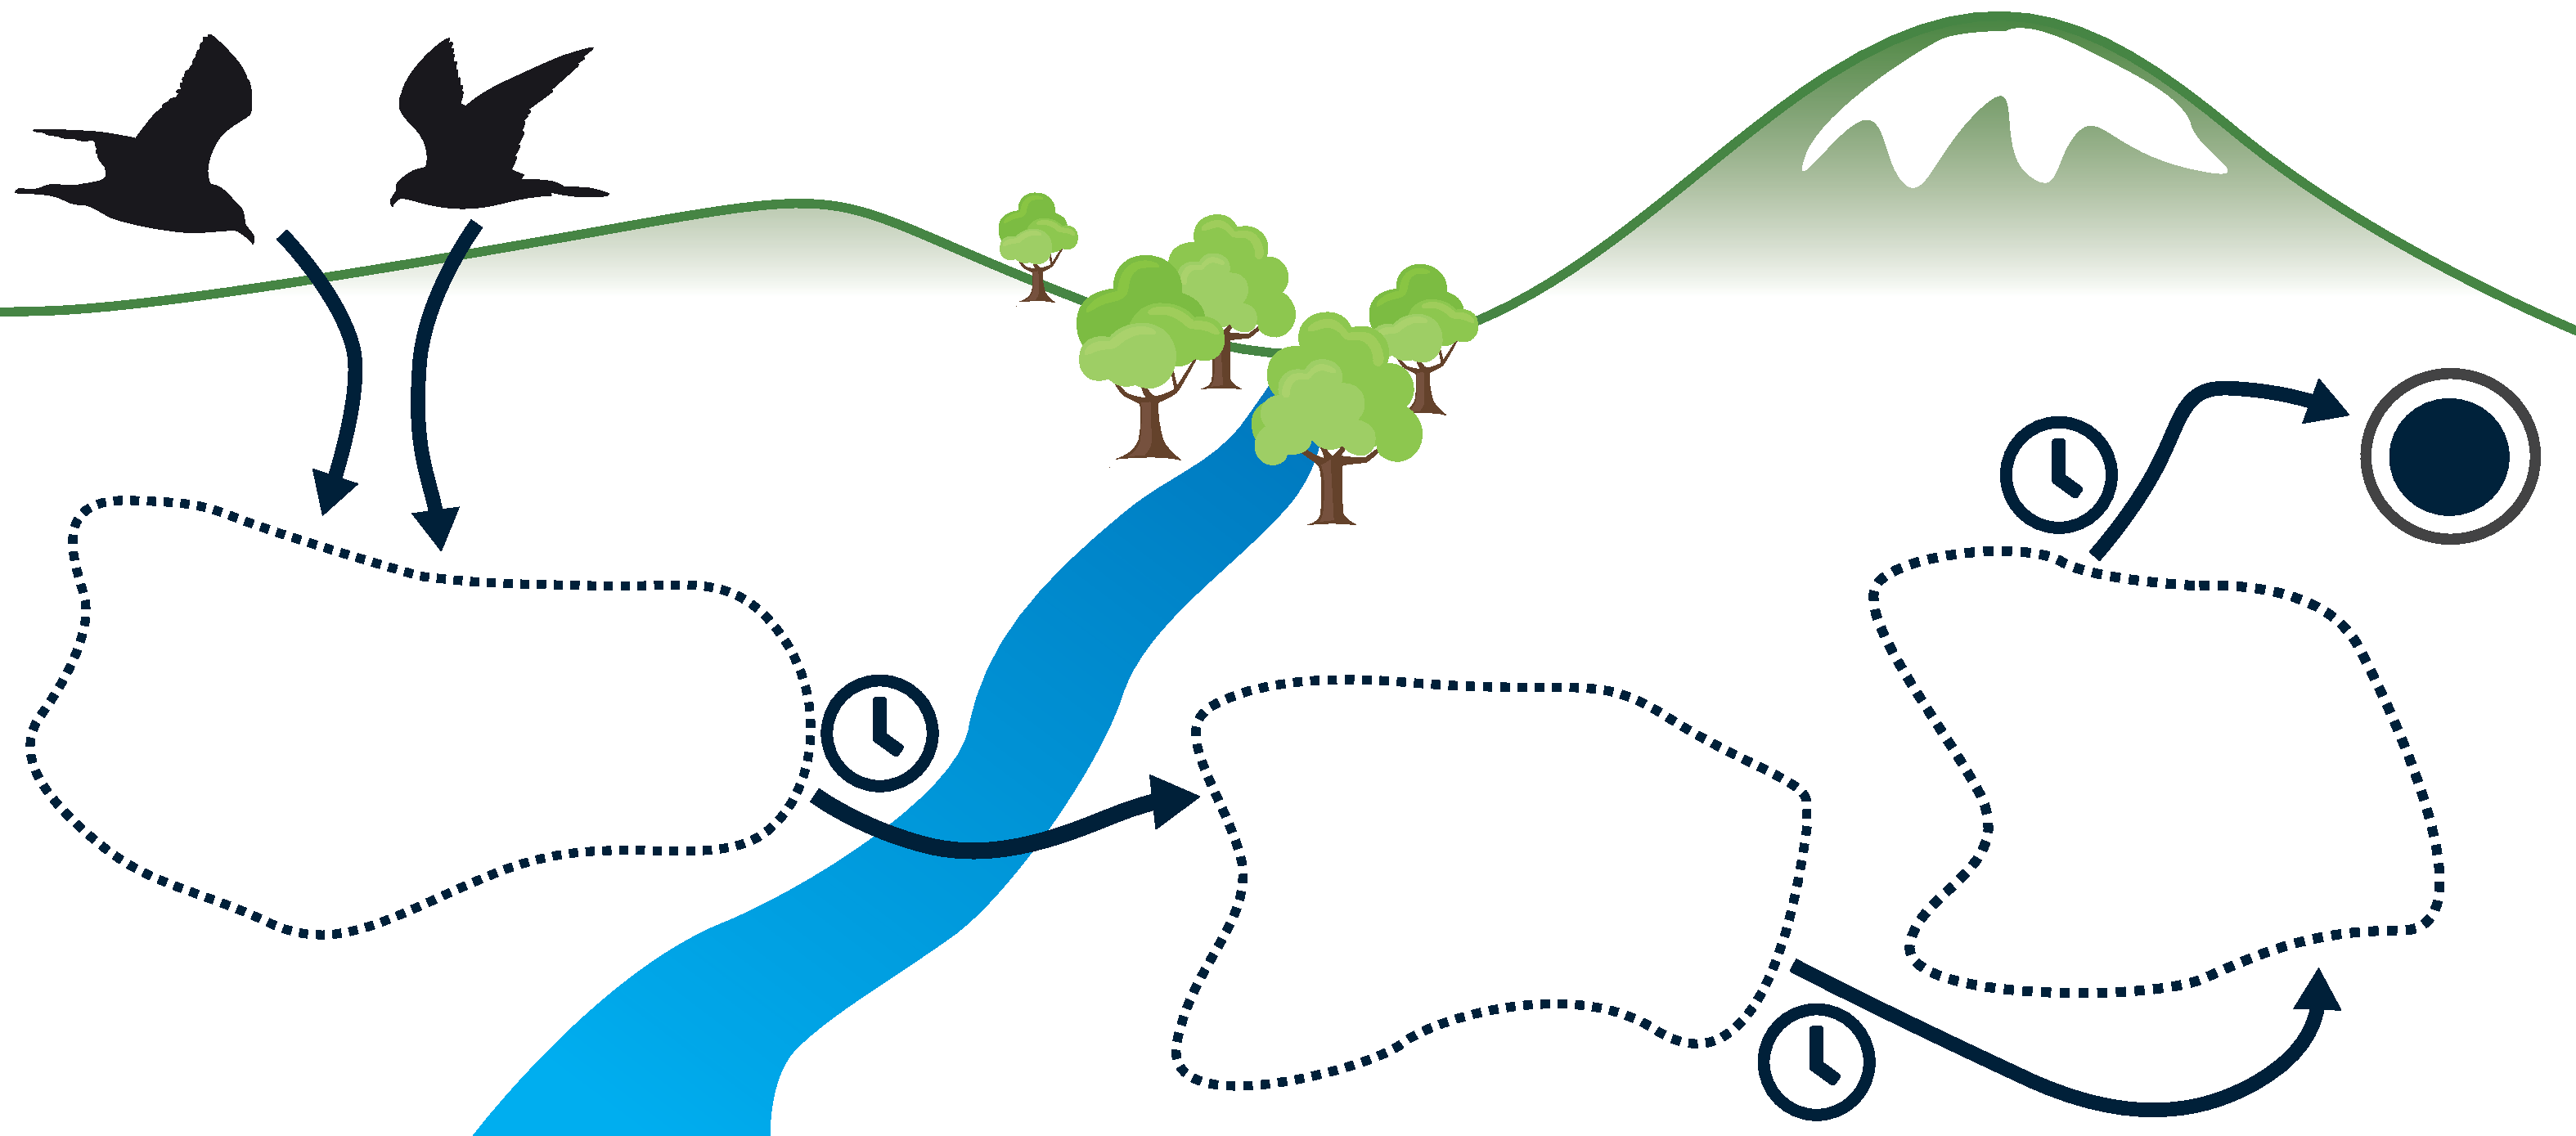
\includegraphics{figures/ch4-gut.pdf}}
    \caption[Give Up Time]{The give up time}
    \label{fig:gut}
\end{figure}

The next two strategies are based on the \emph{time} rule and the \emph{Giving Up} rule~\cite{gibbs1958number_rule}:

\begin{itemize}
    \item[\blueboxbold{SS9}] Employing this stopping strategy, a searcher will leave a SERP after $x_9$ seconds have elapsed from first entering it.
\end{itemize}

\begin{itemize}
    \item[\blueboxbold{SS10}] A searcher employing this strategy will stop after $x_10$ seconds have elapsed since a snippet judged to be relevant was found. If no relevant items have been encountered on the given SERP, then the searcher will stop after $x_9$ seconds have elapsed since arriving at the SERP.
\end{itemize}

These stopping strategies are similar to the frustration based strategies previously proposed (i.e. \textbf{SS2} and \textbf{SS3}) except bound by time~\cite{gibbs1958number_rule}. As mentioned earlier ~\citet{mcnair1982gut_mvt} studied how animals would change their stopping strategies based on their initial evaluation  of the patch, where his suggested combination rule would be as follows.

\begin{itemize}
    \item[\blueboxbold{SS11}] When encountering a SERP expected to yield a high volume of relevant content early on (high scent), the searcher will employ the satisfaction stopping strategy \textbf{SS8S}. If the SERP however yields relevant items over greater depths, or is judged to be of poor quality (low scent), the giving-up stopping strategy, \textbf{SS10G}, is used instead.
\end{itemize}

The combination rule tries to ensure that searcher avoids wasting time on patches with a low yield, but capitalize on patches with a high yield. In the following section, we shall describe the simulated analysis to compare the existing and proposed stopping strategies.

\subsection{\gls{acr:ir} Evaluation Measures}
As previously mentioned most evaluation measures implicitly encode some stopping model (e.g. P$@$10 encodes SS1$@$10). Two measures that have been recently proposed that explicitly encode a stopping model are \textbf{RBP}~\cite{moffat2008rbp} and \textbf{INST}~\cite{bailey2015inst, moffat2015inst}. 
Under \textbf{RBP}, the decision to continue to the next results is based on the patience parameter (e.g. the probability of continuing), while under \textbf{INST} the probability of continuing is based on how many the documents the searcher expects to encounter, how many they have encountered and their current rank - essentially the probability of continuing decreases as they encounter more relevant information, and as they progress further down the ranking.

\begin{itemize}
    \item[\blueboxbold{SS12}] RBP
\end{itemize}

\begin{itemize}
    \item[\blueboxbold{SS13}] INST
\end{itemize}

The satisfaction stopping strategy \textbf{SS8S} was set to consider $1$ to $7$ (hence providing values for $x_8$). A maximum of seven was chosen as this was closest integer to the mean number of documents marked by subjects in the log data. With our \textbf{INST} stopping strategy employing a similar approach, considering the ``number of useful pages that the searcher expects they will need''~\cite{moffat2015inst}, we subsequently set $T$ in INST to the same range. For our other baseline, \textbf{RBP} considers a \emph{patience factor} that influences the depth to which a searcher is prepared to tolerate examining to. Using the log data we estimated the patience of users to be approximately $p=0.9087$. In this study, examined patience from $0.8$ to $0.95$ in steps of $0.05$, and also $0.99$.

\section{General Methodology Overview}\label{sec:csm:methodology}
In Chapters~\ref{chap:snippets} and~\ref{chap:diversity}, we will be exploring how an individual's searching behaviours (particularly their stopping behaviours) vary under differing contexts. This section provides a high level overview of the \emph{general methodology} that we will employ in these two chapters, focusing on four main tasks:

\begin{itemize}
    \item{conducting a \blueboxbold{user study} to examine real-world searcher behaviours;}
    \item{extracting the \blueboxbold{interaction data and performance measures} from the user study;}
    \item{using the aforementioned data to ground a series of \blueboxbold{simulations} that attempt to replicate the user studies; and}
    \item{\blueboxbold{evaluating} the performance of the simulated users, and \blueboxbold{comparing} the simulated user behaviours against those of their real-world counterparts.}
\end{itemize}

We now discuss each of these different tasks in greater depth, highlighting the key decisions and \todo{assumptions} that we have made. Note that this section is directly applicable to contributory Chapters~\ref{chap:snippets} and~\ref{chap:diversity}; Chapter~\ref{chap:serp} provides an in-depth examination on the realism of the~\gls{acr:csm} before we employ it in the following two contributory chapters. Indeed, given that this chapter relies solely on simulations, we follow the approach followed in Section~\ref{chap:csm:method:simulation} and~\ref{chap:csm:method:evaluation}. However, we do ground our experimentation in Chapter~\gls{acr:csm} with user study interaction data from a following chapter.

% Now that we have outlined the~\gls{acr:csm} and the various stopping strategies that we will operationalise, this section provides a high level explanation of the \emph{general methodology} that we will employ in subsequent contributory chapters of this thesis.
%
%
%
% Now that we have outlined the~\gls{acr:csm} and the various stopping strategies that we will operationalise, this section provides a high level explanation of the general methodology of the subsequent contributory chapters. Chapters~\ref{chap:snippets} and~\ref{chap:diversity} will follow this approach, along with the work detailed in Chapter~\ref{chap:serp}.
%
% In essence, the main aim of the following contributory chapters is to examine what happens to a searcher's behaviours (in particular, their stopping behaviours)
%
%
% ground the data
% ground the simulation
% evaluate it later on
% explore influence of these decision points and stopping strategies under different contexts
%
% We want to examine what happens to a searcher's behaviour when different stopping rules are employed under certain contexts.
% How can we do this? Here, we provide a broad overview of the methodology that was employed in the later chapters of this thesis. Broadly split across two main sections.

\subsection{Test Collection, Topics and Search Engine}\label{sec:csm:methodology:collection}
Central to any~\gls{acr:ir} experiment is a corpus of documents (refer to Section~\ref{sec:ir_background:basics:indexing}) with which subjects participating in the experiment can issue queries against. In conjunction with the document corpus, a number of topics are also used to provide simulated information needs.

For the contributory chapters of this thesis, all work detailed uses the TREC AQUAINT corpus, consisting of over one million news articles from the period ranging 1996 to 2000. All of the news articles were collected from three newswires, namely: the \emph{Associated Press (AP);} the \emph{New York Times (NYT);} and \emph{Xinhua}. More contemporary collections could have been used; the reasons for selecting an older were twofold: \emph{(i)} using such a collection enabled us to easily evaluate the performance of subjects; and \emph{(ii)} employing the AQUAINT corpus provides continuity with a prior line of research using this collection, as shown by~\cite{azzopardi2013query_cost}, for example.

Five topics were also selected from the 50 provided in the \emph{TREC 2005 Robust Track,} as outlined by~\cite{voorhees2006trec_robust}. These topics were selected based upon evidence from a previous user study (of similar nature) conducted by~\cite{kelly2015serp_size}. Evidence showed that the topics offered similar levels of difficulty. The five topics, along with a short description of what constitutes a relevant document, are listed below. These summaries are derived from the TREC topic descriptions that are provided as part of the TREC 2005 Robust Track -- Figure~\ref{fig:topics} illustrates three examples of topic descriptions.

\begin{figure}[t!]
    \centering
    \resizebox{1\hsize}{!}{
    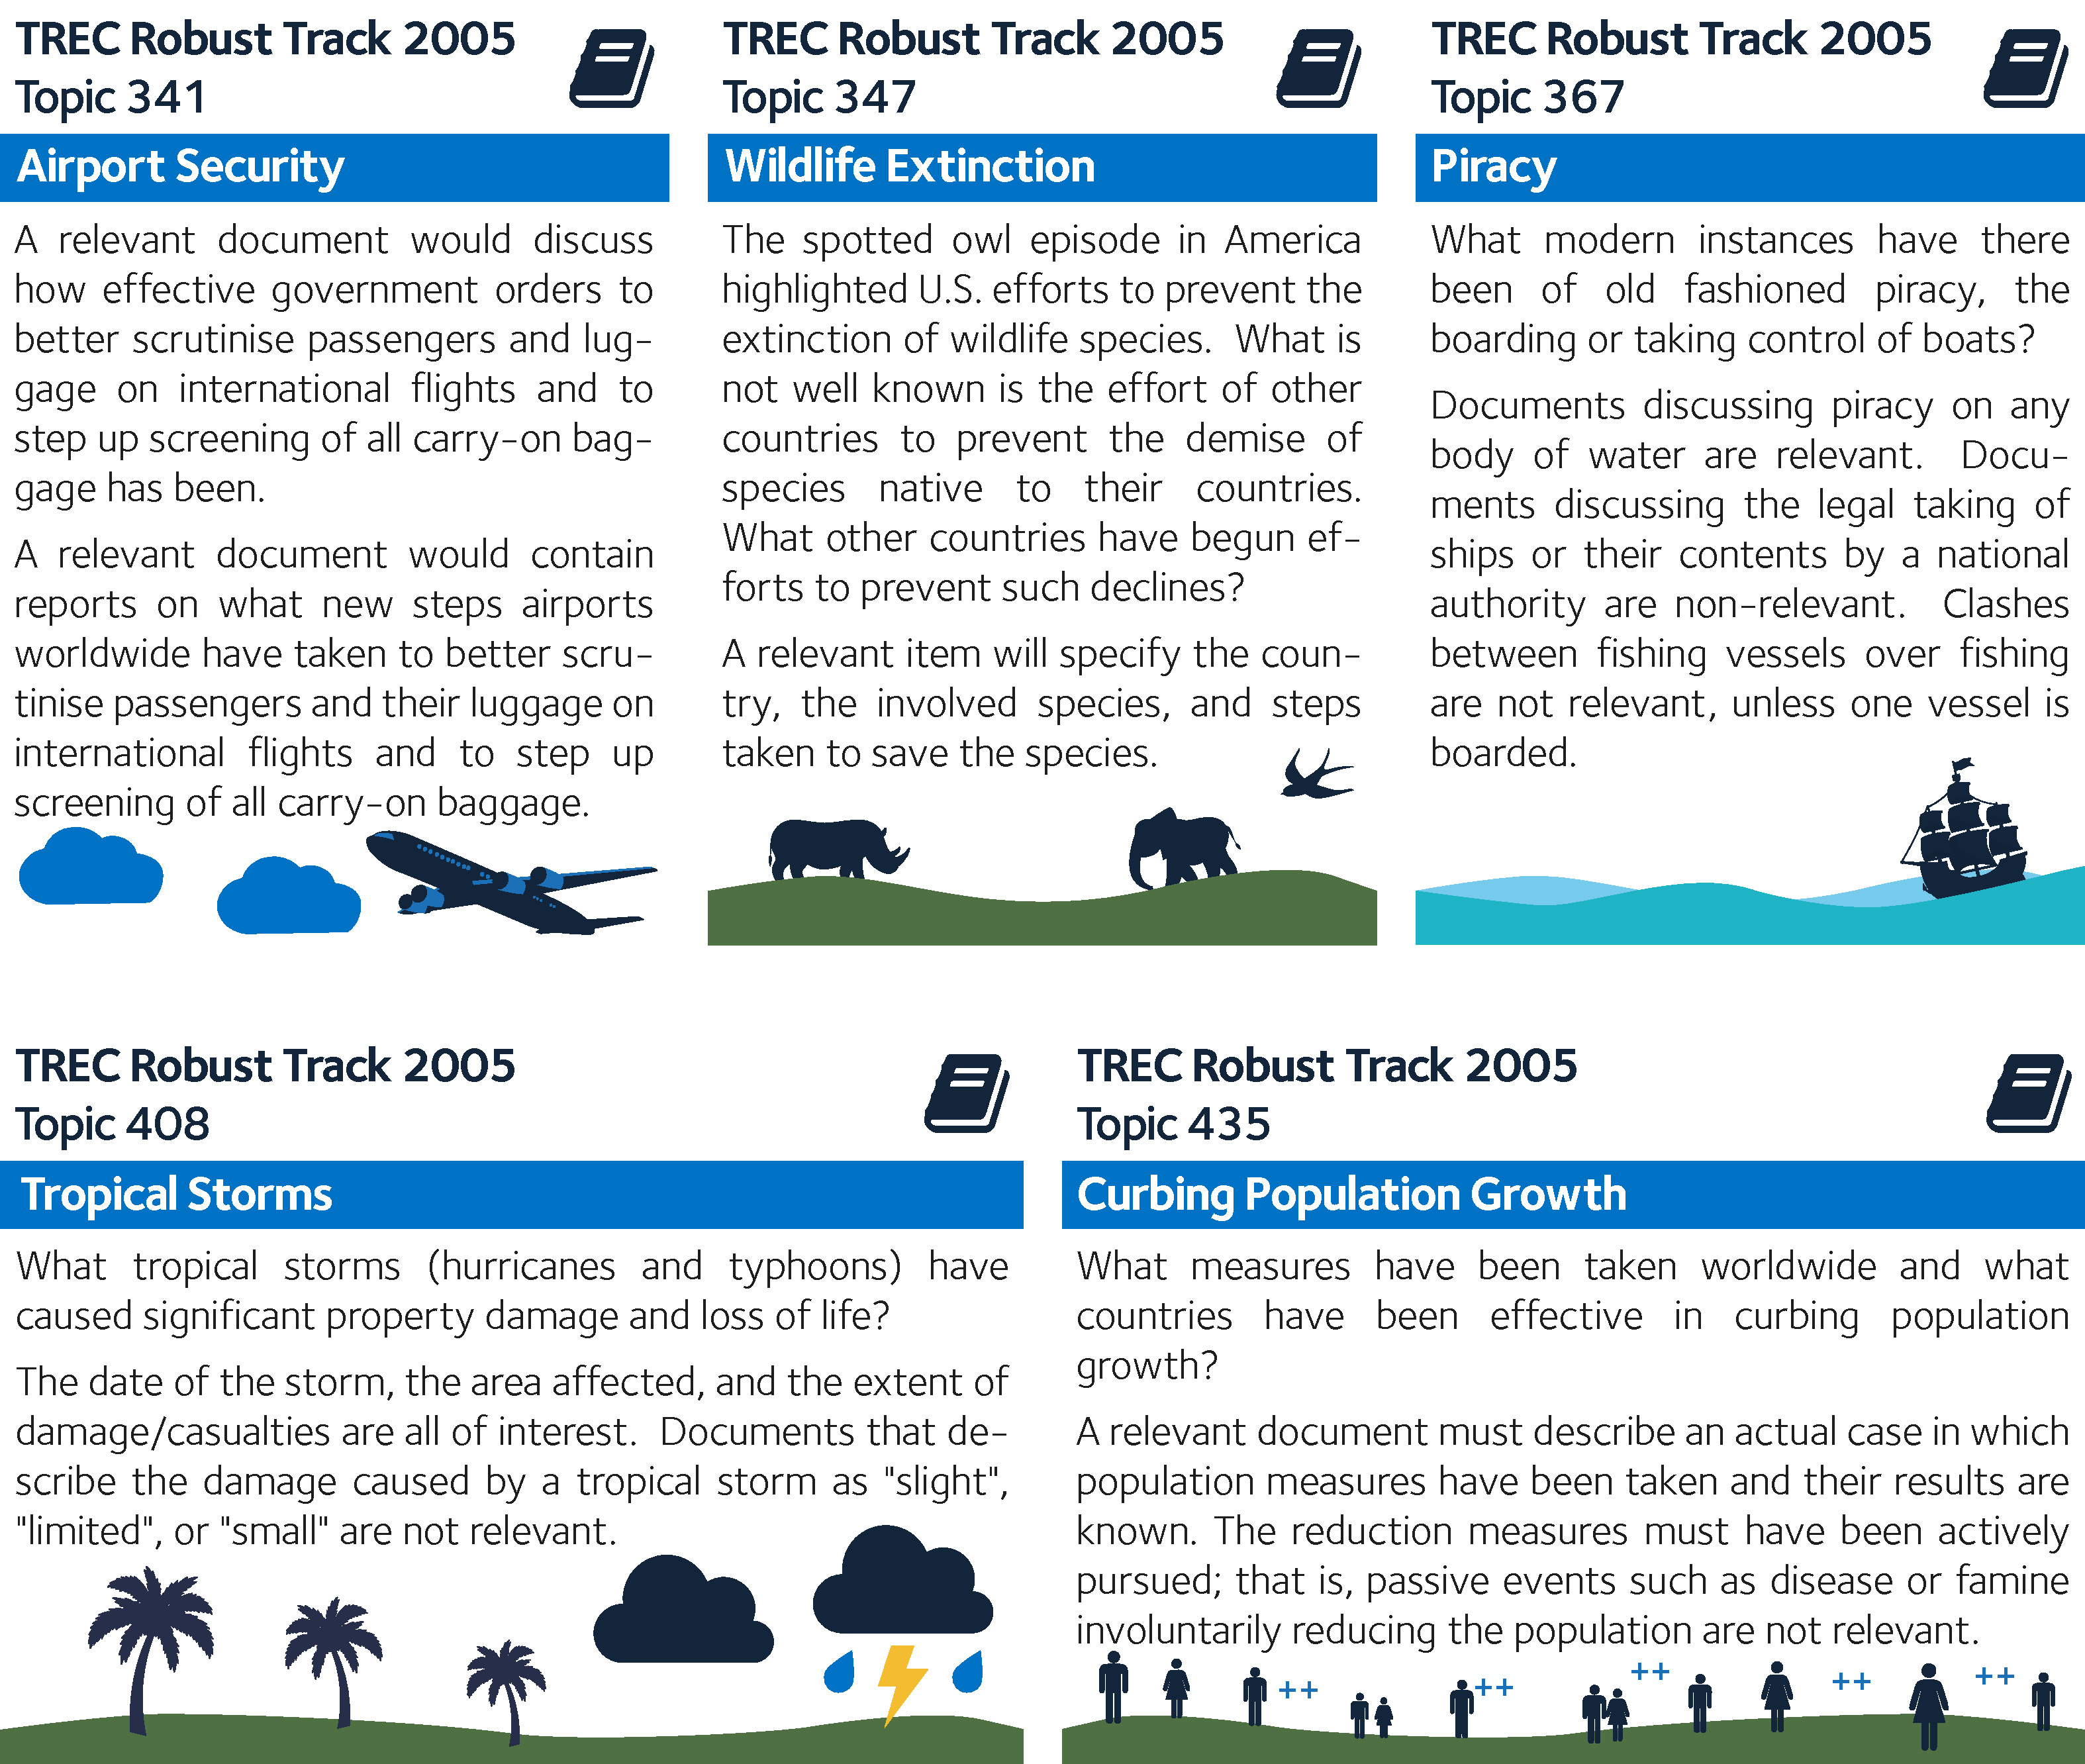
\includegraphics{figures/ch4-topics.pdf}}
    \caption[Examples of TREC Topics]{Three examples of \emph{TREC topic descriptions}, as outlined in Section~\ref{sec:csm:csm:flow}. Topics are extracted from the \emph{TREC 2005 Robust Track,} as outlined by~\cite{voorhees2006trec_robust}. Descriptions provide an explanation as to what constitutes a relevant (and often non-relevant) document.}
    \label{fig:topics}
\end{figure}

\begin{itemize}
    
    \item[]{\blueboxbold{Topic 341 – Airport Security} This topic considers relevant documents as those that discuss additional security measures that were taken by international airports around the world. Relevance is only denoted when a document discusses measures that go beyond the basic passenger and carry-on luggage screening. For example, AQUAINT document \texttt{NYT19980616.0123} discusses \emph{San Francisco International Airport's} attempts at introducing a \emph{robot sniffer,} attempting to look for nitroglycerine in luggage.}
    
    \item[]{\blueboxbold{Topic 347 – Wildlife Extinction} As the title of the topic suggests, this topic concerns wildlife extinction, and what efforts have been taken by countries other than the United States to counter the decline in endangered wildlife. Relevant documents explicitly mention the country, the species of animal, and the efforts the state or other governmental agency took to prevent decline in numbers. For example, document \texttt{XIE20000531.0205} discusses the breeding programme undertaken by China to bolster the number of Siberian Tigers in its jurisdiction.}
    
    \item[]{\blueboxbold{Topic 367 – Piracy} Instances of modern piracy are considered relevant to this topic -- not in the sense of software piracy, but the act of a water going vessel being boarded by individuals wishing to hijack it. Document \texttt{APW19980601.1065} provides an example of this -- the \emph{Petro Ranger}, a large fuel tanker, was boarded by pirates in 1998 in the South China Sea. To be relevant to the topic, the name of the vessel and the body of water it was hijacked on must be mentioned -- those discussing instances of when states intercepted vessels are not relevant.}
    
    \item[]{\blueboxbold{Topic 408 – Tropical Storms} Documents discussing major tropical storms are to be considered relevant, where the storm is reported to have caused significant damage and a large number of casualties. This is a particularly timely topic for the document corpus considered, as the 1998 hurricane season in the Caribbean has been reported to be one of the most costly -- both in terms of damage caused and lives lost -- in history.\footnote{This is reported by the US \emph{National Oceanic and Atmospheric Administration (NOAA),} as seen at \url{http://www.outlook.noaa.gov/98hurricanes/} -- last accessed May 15\textsuperscript{th}, 2018.} Document \texttt{APW19980921.1265} for example discusses the effects on Puerto Rico of Hurricane Georges in September 1998, leaving -- at the time of reporting -- three dead, many houses damaged, and thousands homeless.}
    
    \item[]{\blueboxbold{Topic 435 – Curbing Population Growth} The final topic considers efforts that have been made by countries around the world to control the ever increasing human population. Documents discussing this issue are only relevant to the topic if the results to a case have been made public, and a reduction in population has been actively pursued. The document must mention the country, the As such, events like famines are not relevant. A perhaps well known example of such a phenomenon is the one child policy that was pursued by China in the late 20\textsuperscript{th} century. Document \texttt{NYT19981031.0070} discusses the Chinese government's efforts to curb its expanding population at the time, with sexual education and heavy financial penalties for additional children. These efforts were shown to lead to a reduction in population, although whether this actually occurred is open to debate.}
    
\end{itemize}

For all user studies reported in this thesis, we selected topic \blueboxbold{367} as a \emph{practice topic,} permitting the participating subjects to familiarise themselves with the experimental system used. As such, we do not report any results from interactions that took place with this topic -- comparisons between simulated and actual searcher behaviours are also omitted. 

All queries submitted during experiments were also handled with the \emph{Whoosh~\gls{acr:ir} Toolkit}.\footnote{\emph{Whoosh} can be freely acquired using the \texttt{pip} \emph{Python} package manager -- documentation for Whoosh is available online at \url{http://whoosh.readthedocs.io/en/latest/intro.html} (last accessed May 15\textsuperscript{th}, 2018). The corpus was indexed with Whoosh \texttt{2.7.4}.} Using the toolkit, we indexed the AQUAINT document collection, applying Porter stemming. Stopwords -- from Fox's classical stopword list -- were also removed (refer to Section~\ref{sec:ir_background:basics:indexing} for more information on the indexing process). For this index, we also removed documents with \todo{duplicate titles}. This is an issue, especially with documents originating from a newswire. A document discussing an ongoing event may be continually revised as new information arises, leading to multiple revisions. \todo{For documents with duplicate titles, we retained the document with the latest timestamp.}

With an index weighing in at 800MB, consisting of $128,894$ documents. \todo{What else did we do to reduce this number?} We could then issue queries against the index. All ranked results from queries were computed with the BM25 algorithm, where $\beta=0.75$. Terms in the queries issues were implicitly \texttt{AND}ed together to restrict the set of retrieved documents to those that only contained all of the query terms. This was chosen to reduce the size of the returned set -- most search systems employ such an implicit approach.

\subsection{Conducting a User Study}

- conducted two large scale user studies for the work reported in this thesis.
- chapter x looks at temporal delays
- chapter y looks at the effects of task goals (session level stopping) and the diversification of results
- both examine searcher behaviours.

- using the document collection and topics defined above, we task subjects to find documents 

X
X
X
X

- conditions are explained in more detail in the relevant chapters; refer to Chapters X and Y for more details about the precise setup.

- both user studies were crowdsourced, explain the crowdsourcing stuff.
- using a custom built framework called Treconomics, which has also been used in prior works, such as Azz2013, Max2014.

- framework allows for flexible study design.

- within subjects design, trialled a range of different interfaces and experimental conditions.
- for each interface/condition trialled, we were able to record a variety of information that we discuss below.


\subsection{Extracting User Study Interaction Data}\label{sec:csm:methodology:extracting}
The TREConomics framework provides the necessary infrastructure allowing us to capture a variety of different aspects to how

- framework provided the necessary infrastructure to allow us to capture various aspects relating the how the searchers: behaved, performed, and what their overall experience judgement was.

- the various data sources that we derived our information from are illustrated in Figure~\ref{fig:evaluation_methodology},


- here, we discuss the basic behavioural and performance measures that we obtained, along with a basic overview of the user experience involved. as the components of the user experience component varied considerably between the two studies, we leave detailed explanation of these components until Chapters X and Y.

- in all, behavioural measures can then be used as the \emph{grounding} for our user simulations, which we discuss in Section~\ref{chap:csm:method:simulation}. these were extracted across all different experimental conditions or interfaces trialled, depending upon the considered user study.

% - from the log file, ascertain key data points across the different experimental conditions or interfaces trialled.
% - link back to the complex searcher model section to show where each of the probabilities and costs are used/employed.
% - then, these costs can be fed into simulations, which can then be run (see Section~\ref{sec:proposal:method:simulations} below).

\begin{figure}[t!]
    \centering
    \resizebox{1\hsize}{!}{
    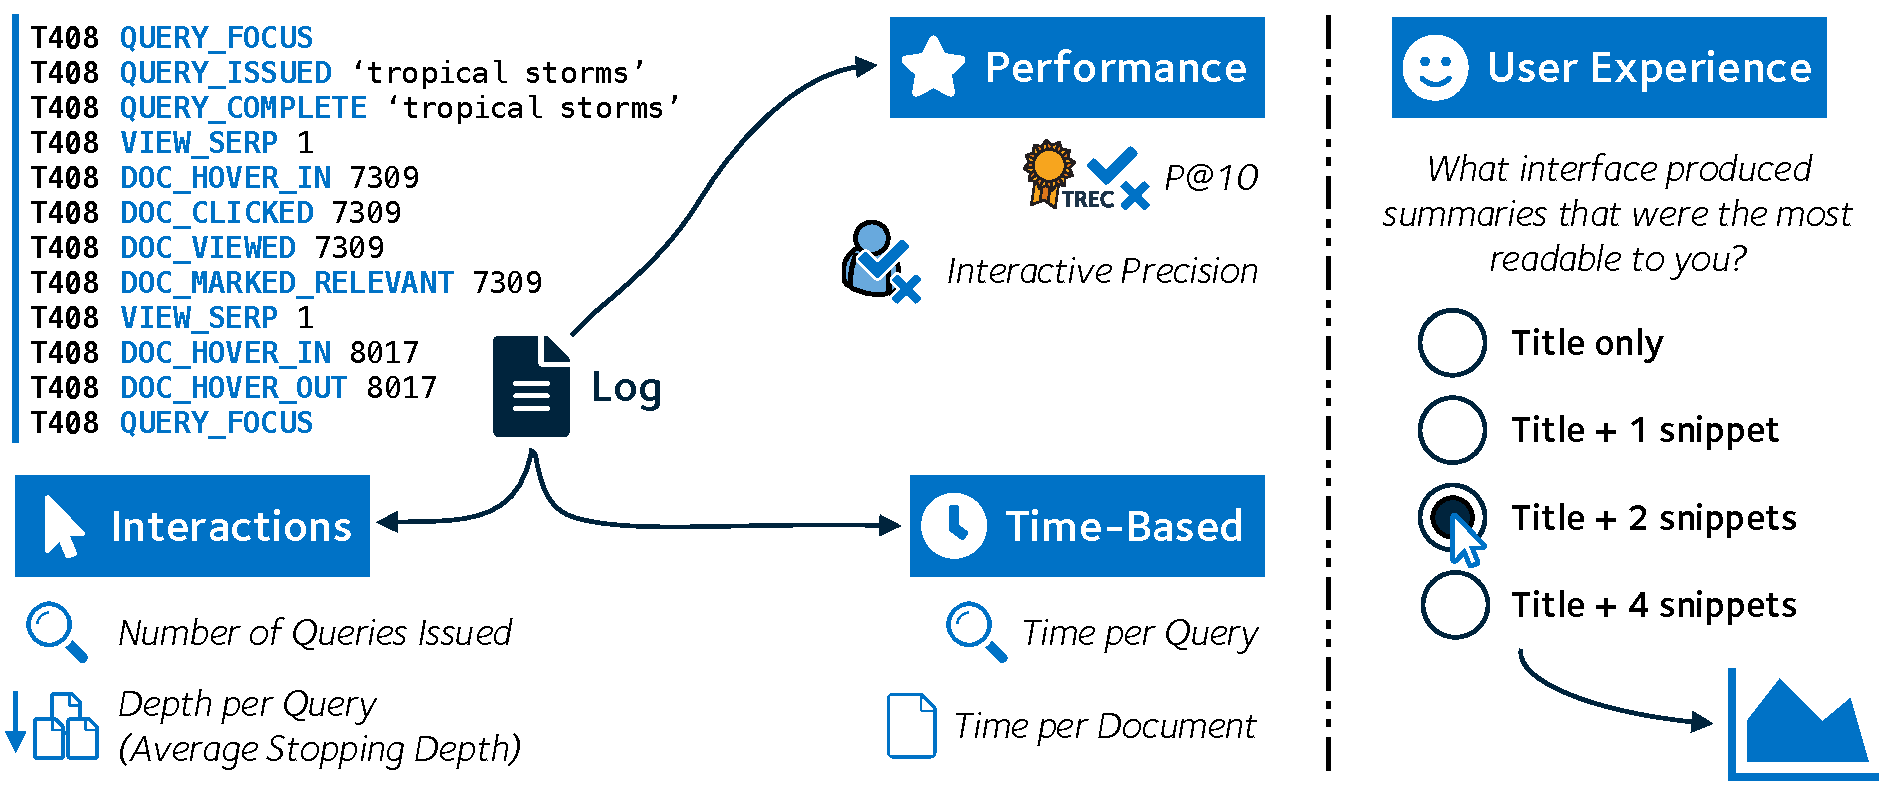
\includegraphics{figures/ch4-evaluation.pdf}}
    \caption[Examples of Evaluation Measures]{An illustration of the different types of measures that are captured, and from what sources. Interaction, time-based and performance measures are derived from the user study experiment log (with TREC QRELs used in conjunction with the interaction log to compute a subject's performance). User experience metrics are collated from a number of different surveys. Refer to Section~\ref{sec:csm:methodology:extracting} for more information.}
    \label{fig:evaluation_methodology}
\end{figure}

\subsubsection{Behavioural Measures}
- recorded from log data.
- a number of different behavioural measures were recorded!

- list from the papers.

\subsubsection{Time-Based Measures}

\subsubsection{Performance Measures}
- as shown from figure~\ref{}, we were also able to extract a number of performance measures, too.
- using the raw data extracted from the interaction log file, we could, in conjunction with an additional evaluation tool (i.e. trec\_eval), use these two resources to calculate measures.

- measures that we considered across both studies included:
- X
- Y
- Z

- used in conjunction with behavioural measures, formed the basis of the seeded experiments.

\subsubsection{User Experience}
- not strictly necessary to forming a grounded simulation.
- but included to ascertain whether subjects perceived a difference between the interfaces and conditions trialled across the two experiments.

- split into five main parts:
    - demographics
    - pre-experiment
    - pre-task
    - post-task
    - post-experiment

- as previously mentioned, many of these components differed across the two studies that were undertaken. as such, we leave explanation of these surveys to each of the chapters.

\subsection{Simulating Searcher Behaviours}\label{chap:csm:method:simulation}
Simulation as defined earlier is a good means for experimentation.
Low cost, always use the same users, no issue of learning bias, etc.

EXPLORE how people's behaviours change

- set up the probabilities
- instantiate the components

- pick a topic set
- pick a corpus
- basic structure of the methodology from previous papers

\subsubsection{Instantiating the Simulations}

\subsubsection{Performance Runs}

\subsubsection{Comparison Runs}

\subsection{Evaluation of Simulations}\label{chap:csm:method:evaluation}
- how do we evaluate how good the system performs?
- how do we work out which one approximates best? on average.

\subsubsection{Determining Simulated User Performance}

\subsubsection{Comparing Simulated and Real-World Subjects}

\section{Chapter Summary}
    %!TEX TS-program = xelatex
%!TEX root = ../../maxwell2018thesis.tex

\chapter[Modelling~\gls{acr:serp} Level Stopping Behaviours]{Modelling~\gls{acr:serp} Level\\Stopping Behaviours}\label{chap:serp}
In Chapters~\ref{chap:snippets} and~\ref{chap:diversity}, we examined the effects of searcher behaviour and performance when experimental interfaces and conditions were varied. This was before proceeding to examine the grounded simulated behaviour and performance of searchers under different snippet level stopping strategies. With the aforementioned considered as the empirical strand of the work reported in this thesis, \blueboxbold{HL-RQ1}\footnote{\blueboxbold{HL-RQ1} is defined in Section~\ref{sec:intro:rqs} on page~\pageref{sec:intro:rqs}.} poses the following overarching research question.

\begin{itemize}
    \item[]{\blueboxbold{HL-RQ1} How can we improve the current state-of-the-art searcher model to incorporate different points where individuals subscribing to such a model can stop?}
\end{itemize}

In order to address this high level research question, we presented in Chapter~\ref{chap:csm} the~\glsfirst{acr:csm}, a conceptual, high level model of the search process. The~\gls{acr:csm} introduced the~\gls{acr:serp} level stopping decision point, motivated by informations scent (refer to Section~\ref{sec:stopping_background:models:theoretical:ift}), allowing simulated searchers subscribing to such a model to \emph{abandon} a~\gls{acr:serp} if a general \emph{overview} of the given~\gls{acr:serp} if the results, from a glance, did not appear to provide promising results. With the definition of the~\gls{acr:csm} partially satisfying \blueboxbold{HL-RQ1}, we in this chapter provide results of an empirical, simulated study of the new stopping decision point, providing evidence that the inclusion of this new stopping decision point does indeed improve simulated searcher performance, and offers closer approximations to how real-world searchers actually behaved.

\section{Motivation and Research Questions}\label{sec:serp:background}
With the background work for this chapter largely outline in Sections~\ref{sec:stopping_background:models:theoretical:ift} and~\ref{sec:csm:new_stopping}, this section provides a refresher of the motivation behind the inclusion of the third, new~\gls{acr:serp} level stopping decision point. We begin with the concept of~\gls{acr:serp} abandonment, before considering how~\glsfirst{acr:ift} provides strong theoretical motivation.

The concept of the new~\gls{acr:serp} level stopping decision point revolves around the concept of~\gls{acr:serp} abandonment, when a searcher fails to click on any of the results returned for a given query~\citep{diriye2012abandonment, hassan2013serp_abandonment}. This may be for a variety of different reasons (both good and bad) -- the primary motivator for this study considers the notion of bad abandonment, where searchers abandon a~\gls{acr:serp} because they are dissatisfied by the results returned~\citep{hassan2013serp_abandonment}.

\begin{figure}[t!]
    \centering
    \resizebox{1\hsize}{!}{
    \includegraphics{figures/ch9-csm.pdf}}
    \caption[The~\glsfirst{acr:csm} and~\gls{acr:serp} stopping point]{The~\glsfirst{acr:csm}, highlighting the stopping decision point (by an asterisk\emph{*}, with the~\gls{acr:serp} examination component also highlighted within the blue rectangle) that is examined in detail in this chapter. Refer to Section~\ref{sec:csm:csm:flow} for an in-depth explanation of the model.}
    \label{fig:csm_ch9}
\end{figure}

Motivated by \emph{information scent} and the \emph{patch model} -- both part of~\glsfirst{acr:ift}\footnote{Refer to Section~\ref{sec:stopping_background:models:theoretical:ift} on page~\pageref{sec:stopping_background:models:theoretical:ift} for a detailed explanation of the patch model.} --~\cite{pirolli1999ift} argue that information seekers are like animals foraging in the wild, and as such will follow a scent to find food. As discussed previously, information seekers have been shown to follow a series of \emph{proximal cues} provided by~\gls{acr:serp} components such as hypertext links, titles, snippets and thumbnails to help locate relevant information~\citep{pirolli1995ift, pirolli1999ift, chi2001information_scent, oltston2003scenttrails, pirolli2007ift}. For example,~\cite{card2001scent_graphs} found that when navigating through webpages, searchers were more likely to leave when the information scent provided on a page began to decline. Work by~\cite{wu2014information_scent} discussed a user study where low, medium and high scent~\glsplural{acr:serp} were created by changing the number and distribution of relevant items on the page -- thus altering the proximal cues provided. Those interacting with high scent~\glsplural{acr:serp} examined more content and went to greater depths compared to those who utilised low scent~\glsplural{acr:serp}. Further work by~\cite{ong2017scent_behaviour} -- and indeed the user study reported in Section~\ref{chap:snippets:user} -- all confirm that modifying the scent of a~\gls{acr:serp} does indeed alter a searcher's stopping behaviour.

For this chapter, we operationalise the information scent as the performance of a given~\gls{acr:serp}, examining how the new~\gls{acr:serp} level stopping decision point within the searcher model -- as shown in Figure~\ref{fig:csm_ch9}\footnote{Further information on the~\glsfirst{acr:csm} can be found in Chapter~\ref{chap:csm}, starting on page~\pageref{chap:csm}.} -- affects searcher, stopping and overall performance. This is achieved by enumerating a series of different~\gls{acr:serp} level stopping strategies, allowing us to operationalise the new stopping decision point in several ways. As such, we pose two key research questions to be addressed in this chapter.

\begin{itemize}
    \item[]{\blueboxbold{RQ1} Does incorporating a~\gls{acr:serp} level stopping decision point lead to higher overall performance?}
    \item[]{\blueboxbold{RQ2} Does incorporating a~\gls{acr:serp} level stopping decision point lead to better approximations of searcher stopping behaviour?}
\end{itemize}

Taken together, the answers to these research questions will in turn provide a complete answer to allow us to address high level \blueboxbold{HL-RQ1}, allowing us to determine whether the inclusion of this additional~\gls{acr:serp} level stopping decision point does improve on the current state-of-the-art. In the next section, we outline the methodology undertaken to address the aforementioned research questions.

\section{Methodology}
In order to address the two research questions posed above, we followed our simulation methodology, outlined in our general methodology chapter. This is detailed in Section~\ref{chap:csm:method:simulation} on page~\pageref{chap:csm:method:simulation}. A variety of different simulation components that mapped to individual components of the~\gls{acr:csm} were left unchanged from the general methodology; this section details the changes to our experimental setup, the key component being the~\gls{acr:serp} level stopping decision point was operationalised for this study.

In this section, we therefore outline:

\begin{itemize}
    \item{the different~\gls{acr:serp} level stopping decision point strategies that were trialled, including the introduction of a new probability of examining a~\gls{acr:serp} (Section~\ref{sec:serp:method:serp_dp});}
    \item{a discussion of the different interaction probabilities and costs that were used for this study (Section~\ref{sec:serp:method:probscosts});}
    \item{an enumeration of the different snippet level stopping strategies trialled for this study (Section~\ref{sec:serp:method:snippet}); and}
    \item{a summary of the other components of the~\gls{acr:csm} that were instantiated in a different way as outlined in the general methodology (Section~\ref{sec:serp:method:other}).}
\end{itemize}

\subsection{\gls{acr:serp} Decision Making}\label{sec:serp:method:serp_dp}
This discusses the various ways in which we implemented this new stopping decision point, allowing us to determine whether it leads to any improvements in overall search performance and better approximations to real-world searcher stopping behaviours.

\blueboxbold{Definition: Low vs. High Scent} First, we must define our interpretation of how the scent of a~\gls{acr:serp} was measured. We follow the work of~\cite{wu2014information_scent}, who stated that a page offering little or no relevant content could be considered to offer a low information scent. As such, our definition of a poor quality~\gls{acr:serp} is defined as $P@10=0.0$. We use this definition to delineate between \emph{good} and \emph{bad}~\glsplural{acr:serp} when considering interaction probabilities below.

\blueboxbold{Probability of Examination} For this new stopping decision point, we introduce the \emph{probability of examining a~\gls{acr:serp}}, or \blueboxbold{P(E)}. This determines how likely it is a searcher will \emph{enter} a~\gls{acr:serp} and begin to examine result summaries in detail. Taking this concept further, we can then consider two additional probabilities that incorporate the notion of a~\glsplural{acr:serp} information scent, yielding:

\begin{itemize}
    \item{\blueboxbold{P(E|HS)}, the probability of examining a~\gls{acr:serp} perceived to give a high information scent (i.e. a good quality~\gls{acr:serp}); and}
    \item{\blueboxbold{P(E|LS)}, the probability of examining a~\gls{acr:serp} offering what appears to be a low information scent (i.e. a poor quality~\gls{acr:serp}, or $P@10=0.0$).}
\end{itemize}

\begin{figure}[t!]
    \centering
    \resizebox{1\hsize}{!}{
    \includegraphics{figures/ch6-serp_probabilities.pdf}}
    \caption[Computing~\gls{acr:serp} examination probabilities]{A simple illustration highlighting how the different~\gls{acr:serp} examination costs were computed. We consider both the probability of examining~\glsplural{acr:serp} yielding both high and low information scents. Definitions are used from~\cite{wu2014information_scent} and~\cite{hassan2013serp_abandonment}.}
    \label{fig:serp_probabilities}
\end{figure}

These values were computed from interaction log data, derived from the two user studies discussed in Chapters~\ref{chap:snippets} and~\ref{chap:diversity}. Values derived are not reported in this section; refer to Section~\ref{sec:serp:method:probscosts} for the probabilities extracted. Intuitively however, one would expect a searcher demonstrating competency at searching for information to know when a query is returning good results, and vice versa. As such, one would expect to see a higher probability for $P(E|HS)$ than when compared to $P(E|LS)$, and would thus provide evidence that searchers do indeed attempt to avoid low quality~\glsplural{acr:serp}.

As illustrated in Figure~\ref{fig:serp_probabilities}, we took each query issued from the interaction log, and extracted for each the $P@10$ score (as per~\cite{wu2014information_scent}). If $P@10=0.0$, the associated~\gls{acr:serp} for the query would have offered a low information scent. Conversely, if $P@10 > 0.0$, the information scent would have been considered to be high. For the interactions recorded on each~\gls{acr:serp}, we could then count the number that recorded no clicks (or no result summaries deemed to be attractive enough to examine further). We considered this as a definition of an \emph{abandoned~\gls{acr:serp}}, as used in previous work by~\cite{hassan2013serp_abandonment}. From these counts, we could then compute the probabilities of examining a~\gls{acr:serp}, as illustrated in Figure~\ref{fig:serp_probabilities}.

\blueboxbold{Considering Browser Viewport Size}
We now turn our attention to how a simulated searcher is able to make a judgement of the presented~\gls{acr:serp}. As we discussed previously in Section~\ref{sec:serp:background}, real-world searchers are able to infer the quality (and perhaps relevance) of a given page or~\gls{acr:serp} through the examination of various proximal cues~\citep{chi2001information_scent}.

\begin{wrapfigure}[13]{r}{0.45\textwidth}
    \begin{center}
    \vspace*{-9mm}
    \includegraphics[width=1\textwidth]{figures/ch6-viewport.pdf}
    \end{center}
    \vspace*{-2mm}
    \caption[Viewport cutoff example]{The~\gls{acr:serp} viewport threshold. In this example, three result summaries are visible, with two present but outwith the viewport. Therefore, \emph{v\textsubscript{size}=3}. Cheers!}
    \label{fig:viewport_cutoff}
\end{wrapfigure}

While we do not specifically examine different cues, instead relying on more simplistic means to operationalise the stopping decision point, we nevertheless do consider the \emph{size of the browser's viewport}. A~\gls{acr:serp} is typically larger than the viewport it is displayed within, which leads to the inclusion of scrollbars. Results can only be seen \emph{above-the-fold}, or what is visible within the viewport. We argue that a searcher can infer the quality of the~\gls{acr:serp} from the initial view they are presented with, and thus incorporate a \emph{viewport size} ($v_{size}$) variable in our implementations. A searcher can only judge what they can see. This variable can vary between the different interfaces we trialled -- for example, longer snippet text results in fewer result summaries being displayed in the initial view. By using a fixed-size popup window in the two user studies (as discussed in Section~\ref{sec:csm:methodology:user:interface}), we were then able to manually check the number of result summaries displayed within the popup window, and use these values to ground the new stopping decision point further.

For our simulations, we use different values of $v_{size}$ over the study interfaces reported in Chapter~\ref{chap:snippets} only. This is because introducing longer result summaries would mean fewer overall would be displayed within a viewport of the same size. Across the experimental conditions trialled in Chapter~\ref{chap:diversity}, $v_{size}$ remains constant as result summary lengths were not modified. Values used for $v_{size}$ are reported later in Section~\ref{sec:serp:method:probscosts}.

\subsubsection{Decision Point Implementations}\label{sec:serp:method:serp_dp:implementations}
We trialled three different implementations of the~\gls{acr:serp} level stopping decision point, providing us with the ability to determine the effect of incorporating it within the~\gls{acr:csm}. These are enumerated below, with an explanation of each. The first can be considered our simple baseline approach.

\begin{itemize}
    \item{\blueboxbold{Always Examine (Baseline)} With this approach, a searcher will \emph{always enter} the~\gls{acr:serp}, and examine at least one result summary -- the exact number would be determined by the snippet level stopping strategy. This is the current state-of-the-art, and we consider this as our baseline. Indeed, this strategy was used in the simulations reported in Chapters~\ref{chap:snippets} and~\ref{chap:diversity}.}
\end{itemize}

From here, the remaining two strategies begin to consider a simulated searcher's judgements regarding the perceived quality of a~\gls{acr:serp}, and thus begin to use the new stopping decision point to abandon a~\gls{acr:serp} before examining individual result summaries in detail.

\begin{itemize}
    \item{\blueboxbold{Perfect~\gls{acr:serp} Judgements} Here, a simulated searcher will only begin to examine a~\gls{acr:serp} in detail if $P@v_{size} > 0$ (considering the viewport size). If $P@v_{size} = 0$, the searcher will abandon the~\gls{acr:serp}, and proceed to the next action as dictated by the~\gls{acr:csm}. This is the upper bound in terms of performance for the stopping decision point, and is analogous to, as an example, the \emph{ideal user} of~\cite{hagen2016simulating_users}.}
    \item{\blueboxbold{Stochastic~\gls{acr:serp} Judgements} This implementation used a stochastic element to determine whether the simulated searcher should enter the~\gls{acr:serp} or not. Like above, the viewport size ($P@v_{size}$) of the~\gls{acr:serp} is computed. If the~\gls{acr:serp} is of high scent, $P(E|HS)$ is used to determine whether the searcher should enter the~\gls{acr:serp}. Conversely, if the~\gls{acr:serp} is considered to be of low scent, $P(E|LS)$ is used instead to determine the likelihood of abandonment. We considered three different sets of probabilities for the stochastic implementation.}
    
    \begin{itemize}
        \item{\blueboxbold{Average} $P(E|HS)$ and $P(E|LS)$ are estimated over all subjects of a particular interface or condition.}
        \item{\blueboxbold{Savvy} $P(E|HS)$ and $P(E|LS)$ are estimated based upon the top 15 subjects for a particular interface/condition with the \emph{lowest} $P(E|LS)$.}
        \item{\blueboxbold{Na\"{i}ve} $P(E|HS)$ and $P(E|LS)$ are estimated based upon the top 15 subjects for a particular interface/condition with the \emph{highest} $P(E|LS)$.}
    \end{itemize}
\end{itemize}

By considering these different approaches to implementing the new~\gls{acr:serp} level stopping decision point, we can then clearly identify whether it can offer improved performance and approximations of actual searcher stopping behaviours. We also run each of the stochastic~\gls{acr:serp} level stopping decision components a total of \todo{$30$} times, computing the average over the different trials.

\subsection{Interfaces, Conditions, and Experimental Grounding}\label{sec:serp:method:probscosts}
To determine whether the new~\gls{acr:serp} level stopping decision points offers improvements across a variety of different interfaces and conditions (and can therefore considered to be generalisable), we conducted a series of simulations across the eight interface and experimental conditions trialled in the two user studies, reported in Chapters~\ref{sec:snippets} and~\ref{sec:diversity}.

\begin{table}[t!]
    \caption[Experimental interfaces and conditions]{Experimental interfaces and conditions trialled in this chapter, based upon the work reported in Chapters~\ref{chap:snippets} and~\ref{chap:diversity}. In total, eight different experimental interfaces and conditioned were trialled, considering different result summary lengths, systems and tasks.}
    \label{tbl:serp_conditions}
    \renewcommand{\arraystretch}{1.8}
    \begin{center}
    \begin{tabulary}{\textwidth}{L{0.4cm}@{\CS}L{3.2cm}@{\CS}D{3.51cm}@{\CS}D{3.51cm}@{\CS}D{3.51cm}@{\CS}}

        \RS & & \lbluecell \textbf{Summary Length} & \lbluecell \textbf{System} & \lbluecell \textbf{Task} \\

        \RS \multirow{4}{*}{\rotatebox{90}{\hspace*{-4mm}\textbf{Chapter~\ref{chap:snippets}}}} & \lbluecell\textbf{T0} & \cell \small{Title only} & \cell \small{\blueboxbold{ND} (Non Div.)} & \cell \small{\darkblueboxbold{AD} (Ad-hoc)}\\
        \RS & \lbluecell\textbf{T1} & \cell \small{Title + 1 snippet} & \cell \small{\blueboxbold{ND} (Non Div.)} & \cell \small{\darkblueboxbold{AD} (Ad-hoc)}\\
        \RS & \lbluecell\textbf{T2} & \cell \small{Title + 2 snippets} & \cell \small{\blueboxbold{ND} (Non Div.)} & \cell \small{\darkblueboxbold{AD} (Ad-hoc)}\\
        \RS & \lbluecell\textbf{T4} & \cell \small{Title + 4 snippets} & \cell \small{\blueboxbold{ND} (Non Div.)} & \cell \small{\darkblueboxbold{AD} (Ad-hoc)}\\
        
        \RS\RS\RS \multirow{4}{*}{\rotatebox{90}{\hspace*{-4mm}\textbf{Chapter~\ref{chap:diversity}}}} & \lbluecell\textbf{D-AS} & \cell \small{Title + 2 snippets} & \cell \small{\blueboxbold{D} (Div.)} & \cell \small{\darkblueboxbold{AS} (Aspectual)}\\
        \RS & \lbluecell\textbf{ND-AS} & \cell \small{Title + 2 snippets} & \cell \small{\blueboxbold{ND} (Non Div.)} & \cell \small{\darkblueboxbold{AS} (Aspectual)}\\
        \RS & \lbluecell\textbf{D-AD} & \cell \small{Title + 2 snippets} & \cell \small{\blueboxbold{D} (Div.)} & \cell \small{\darkblueboxbold{AD} (Ad-hoc)}\\
        \RS & \lbluecell\textbf{ND-AD} & \cell \small{Title + 2 snippets} & \cell \small{\blueboxbold{ND} (Non Div.)} & \cell \small{\darkblueboxbold{AD} (Ad-hoc)}\\
        
    \end{tabulary}
    \end{center}
\end{table}

From Chapter~\ref{chap:snippets}, the four different experimental interfaces -- whereby result summary lengths were manipulated -- are considered. Namely, these are \blueboxbold{T0}, \blueboxbold{T1}, \blueboxbold{T2} and \blueboxbold{T4}. From Chapter~\ref{chap:diversity}, we also considered the four experimental conditions that manipulated the underlying system and searcher tasks: \dualbluebox{D}{AS}, \dualbluebox{ND}{AS}, \dualbluebox{D}{AD} and \dualbluebox{ND}{AD}. The eight interfaces and conditions trialled are presented in Table~\ref{tbl:serp_conditions}, complete with an explanation of the differences between each.

\begin{table}[t!]
    \caption[Simulation interaction probabilities and v\textsubscript{size}]{Probabilities of examining high \emph{P(E|HS)} and low scent~\glsplural{acr:serp} \emph{P(E|LS)}, along with \emph{v\textsubscript{size}} values for each of the eight different experimental interfaces and conditions trialled, reported over three different set of probabilities. Refer to Tables~\ref{tbl:snippets_simulation_probcosts} (page~\pageref{tbl:snippets_simulation_probcosts}) and~\ref{tbl:diversity_simulation_probcosts} (page~\pageref{tbl:diversity_simulation_probcosts}) for other interaction probabilities and costs for studies reported in Chapters~\ref{chap:snippets} and~\ref{chap:diversity} respectively.}
    \label{tbl:serp_probs_costs}
    \renewcommand{\arraystretch}{1.8}
    \begin{center}
    \begin{tabulary}{\textwidth}{L{0.4cm}@{\CS}L{3.2cm}@{\CS}D{2.5cm}@{\CS}D{2.5cm}@{\CS}D{2.5cm}@{\CS}D{2.5cm}@{\CS}}

        \RS & \dbluecell \textbf{Chapter~\ref{chap:snippets}} & \lbluecell \textbf{T0} & \lbluecell \textbf{T1} & \lbluecell \textbf{T2} & \lbluecell \textbf{T4} \\
        
        \RS \multirow{2}{*}{\rotatebox{90}{\hspace*{-2mm}\textbf{Average}}} & \lbluecell\textbf{P(E|HS)} & \cell \small{xx} & \cell \small{xx} & \cell \small{xx} & \cell \small{xx}\\
        \RS & \lbluecell\textbf{P(E|LS)} & \cell \small{xx} & \cell \small{xx} & \cell \small{xx} & \cell \small{xx}\\
        
        \RS\RS\RS \multirow{2}{*}{\rotatebox{90}{\hspace*{-2mm}\textbf{Savvy}}} & \lbluecell\textbf{P(E|HS)} & \cell \small{xx} & \cell \small{xx} & \cell \small{xx} & \cell \small{xx}\\
        \RS & \lbluecell\textbf{P(E|LS)} & \cell \small{xx} & \cell \small{xx} & \cell \small{xx} & \cell \small{xx}\\
        
        \RS\RS\RS \multirow{2}{*}{\rotatebox{90}{\hspace*{-2mm}\textbf{Na\"{i}ve}}} & \lbluecell\textbf{P(E|HS)} & \cell \small{xx} & \cell \small{xx} & \cell \small{xx} & \cell \small{xx}\\
        \RS & \lbluecell\textbf{P(E|LS)} & \cell \small{xx} & \cell \small{xx} & \cell \small{xx} & \cell \small{xx}\\
        
        \RS\RS\RS & \lbluecell\textbf{v\textsubscript{size}} & \cell \small{10} & \cell \small{9} & \cell \small{7} & \cell \small{6}\\
        
        \RS\RS\RS\RS\RS\RS & \dbluecell \textbf{Chapter~\ref{chap:diversity}} & \lbluecell \textbf{D-AS} & \lbluecell \textbf{ND-AS} & \lbluecell \textbf{D-AD} & \lbluecell \textbf{ND-AD} \\
        
        \RS \multirow{2}{*}{\rotatebox{90}{\hspace*{-2mm}\textbf{Average}}} & \lbluecell\textbf{P(E|HS)} & \cell \small{xx} & \cell \small{xx} & \cell \small{xx} & \cell \small{xx}\\
        \RS & \lbluecell\textbf{P(E|LS)} & \cell \small{xx} & \cell \small{xx} & \cell \small{xx} & \cell \small{xx}\\
        
        \RS\RS\RS \multirow{2}{*}{\rotatebox{90}{\hspace*{-2mm}\textbf{Savvy}}} & \lbluecell\textbf{P(E|HS)} & \cell \small{xx} & \cell \small{xx} & \cell \small{xx} & \cell \small{xx}\\
        \RS & \lbluecell\textbf{P(E|LS)} & \cell \small{xx} & \cell \small{xx} & \cell \small{xx} & \cell \small{xx}\\
        
        \RS\RS\RS \multirow{2}{*}{\rotatebox{90}{\hspace*{-2mm}\textbf{Na\"{i}ve}}} & \lbluecell\textbf{P(E|HS)} & \cell \small{xx} & \cell \small{xx} & \cell \small{xx} & \cell \small{xx}\\
        \RS & \lbluecell\textbf{P(E|LS)} & \cell \small{xx} & \cell \small{xx} & \cell \small{xx} & \cell \small{xx}\\
        
        \RS\RS\RS & \lbluecell\textbf{v\textsubscript{size}} & \cell \small{7} & \cell \small{7} & \cell \small{7} & \cell \small{7}\\
        
    \end{tabulary}
    \end{center}
\end{table}

Table~\ref{tbl:serp_probs_costs} presents the probabilities of examining~\glsplural{acr:serp} yielding low ($P(E|LS)$) and high ($P(E|HS)$) scents. Values are computed as per the explanations provided in Section~\ref{sec:serp:method:serp_dp}. The table reports values across each of the eight different experimental interfaces and conditions trialled. In addition, values are reported for each interface and condition across the three different probability sets of \emph{average, savvy} and \emph{na\"{i}ve} searchers (as discussed in Section~\ref{sec:serp:method:serp_dp:implementations}). Also included within the table are the $v_{size}$ values used across each interface or condition, denoting the number of result summaries within a simulated viewport.

These values should be considered in tandem with the interaction costs and probabilities presented in Tables~\ref{tbl:snippets_simulation_probcosts} (presented on page~\ref{tbl:snippets_simulation_probcosts}) and~\ref{tbl:diversity_simulation_probcosts} (presented on page~\pageref{tbl:diversity_simulation_probcosts}) for other classical interaction probabilities (considering the probabilities of marking result summaries, $P(C|R)$ and $P(C|N)$ -- and saving documents, $P(S|R)$ and $P(S|N)$) and interaction costs (including the cost of: querying; examining a~\gls{acr:serp}; examining a result summary; examining a document; and saving a document) for the studies reported in Chapters~\ref{chap:snippets} and~\ref{chap:diversity} respectively. Table~\ref{tbl:serp_probs_costs} reports only the probabilities of examining a~\gls{acr:serp}.

\subsection{Snippet Level Stopping Strategies}\label{sec:serp:method:snippet}
Chapter~\ref{chap:strategies} presented thirteen different snippet level stopping strategies. To reduce the complexity of the experimentation reported in this chapter, we decided to reduce the number of snippet level stopping strategies that we considered. Doing so reduced the risk of potentially repeating the same results as shown before, while still demonstrating that when enabled, the~\gls{acr:serp} level stopping decision point yielded improved performance and closer approximations to actual searcher stopping behaviour over a range of configurations.

As such, we report over the following \todo{six} snippet level stopping strategies in this chapter. These were selected as they offered good performance and approximations of actual searcher stopping behaviours in results presented in previous chapters.

\begin{itemize}
    \item{\blueboxbold{SS1}}
    \item{\blueboxbold{SS2}}
    \item{\blueboxbold{SS3}}
    \item{\blueboxbold{SS4}}
    \item{\blueboxbold{SS5}}
    \item{\blueboxbold{SS6}}
\end{itemize}

Note that these strategies were instantiated with the same $x_n$ values as reported in the general methodology in Section~\ref{chap:csm:method:simulation:grounding:stopping_strats} on page~\pageref{chap:csm:method:simulation:grounding:stopping_strats}.

\subsection{Remaining~\gls{acr:csm} Components}\label{sec:serp:method:other}
We considered only the query generation strategy \blueboxbold{QS3\textsuperscript{+}}, as outlined in Section~\ref{chap:csm:method:simulation:grounding:querying} (page~\pageref{chap:csm:method:simulation:grounding:querying}) for use in the performance runs. This helped to simplify and reduce the number of experimental runs required. For comparison runs, queries issued by real-world subjects under each of the eight experimental interfaces and conditions were again \emph{replayed}, as discussed in Section~\ref{chap:csm:method:sim:runs:comparison} on page~\pageref{chap:csm:method:sim:runs:comparison}.

For the four experimental interfaces trialled in the study reported in Chapter~\ref{chap:snippets}, the same experimental methodology was followed as described in Section~\ref{sec:snippets:simulations:method}. Similarly, the same experimental method was followed as reported in Section~\ref{sec:diversity:simulated:method} for the four experimental conditions belonging to the studies reported in Chapter~\ref{chap:diversity}.

\section{Results}

\subsection{Performance Runs}

\subsection{User Comparison Runs}

\section{Discussion and Chapter Summary}

    %!TEX TS-program = xelatex
%!TEX root = ../../maxwell2018thesis.tex

\part[Examining Searcher Stopping Behaviours]{In this part of the thesis, we present our \darkbluebox{empirical contributions}, examining what happens to searcher stopping behaviours under \darkbluebox{different search contexts}. We then report on a number of different \darkbluebox{simulated analyses}, examining our proposed stopping strategies. Finally, we report on an empirical analysis of the new \darkbluebox{SERP level stopping decision point}.}{Examining and Simulating Searcher Stopping Behaviours}\label{part:context}
    %!TEX TS-program = xelatex
%!TEX root = ../../maxwell2018thesis.tex

\chapter[The Effect of Temporal Delays on Stopping Behaviour]{The Effect of Temporal Delays\\on Stopping Behaviour}\label{chap:temporal}

\begin{publications_box}{Associated Publication}
This chapter is based upon work presented in the following publication.
\vspace*{-3mm}
\begin{itemize}
    \item{\bibentry{maxwell2014temporal_delays}}
\end{itemize}
\end{publications_box}

\section{The Effects of Temporal Delays}

\section{Simulated Analysis}

\section{Chapter Summary}
    %!TEX TS-program = xelatex
%!TEX root = ../../maxwell2018thesis.tex

\chapter[Snippet Lengths and Stopping Behaviour]{Snippet Lengths and\\Stopping Behaviour}\label{chap:snippets}
One of the primary components of a retrieval system that searchers interact with the~\glsfirst{acr:serp}. The presentation and design of the~\gls{acr:serp} has over the years been subject to much research. With more complex components now becoming commonplace in contemporary web search engines (such as the \emph{information card}~\citep{navalpakkam2013non_linear_serp, bota2016information_cards} or \emph{social annotations}~\citep{muralidharan2012social_annotations}), much work however still remains on examining how more traditional~\gls{acr:serp} components, such as \emph{result summaries,} are designed and presented to searchers.

\begin{figure}[h]
    \centering
    \vspace{4mm}
    \resizebox{1\hsize}{!}{
    \includegraphics{figures/ch7-serpintro.pdf}}
    \label{fig:serpintro}
    \vspace{-5mm}
\end{figure}

Result summaries (an example of which is shown above) have been traditionally viewed as the \emph{ten blue links}, each with their corresponding title and source (typically a~\gls{acr:url}) of the document. Included with these two components are the textual \emph{snippets} of \emph{keywords-in-context}, derived from the document itself. These snippets are approximately 130-150 characters (or two lines) in length~\citep{hearst2009_search}. Numerous researchers have explored result summaries in a variety of different ways, such as: examining their length~\citep{paek2004wavelens,cutrell2007eye_tracking,kaisser2008improving}; the use of thumbnails~\citep{woodruff2002summaries,teevan2009visual_snippets}; their attractiveness~\citep{clarke2007caption_features,he2012bridging}; and the generation of \emph{query-biased snippets}~\citep{tombros1998query_biased,rose2007snippet_attributes}. The performance of searchers has broadly been evaluated in a limited fashion (for example, by examining task completion times).

In this chapter, we are interested in examining how the length (and subsequently information content) of result summaries affects~\gls{acr:serp} interactions -- specifically examining their stopping behaviours -- and a searcher's ability to select relevant over non-relevant items. Prior research has demonstrated that longer result summaries tend to lower completion times for informational tasks, where searchers need to find only a single relevant document~\citep{cutrell2007eye_tracking}. Does this finding however hold in an ad-hoc context, where searchers need to find \emph{several} relevant items? Furthermore, how does the length and information associated with longer result summaries affect the searcher's ability to discern the relevant from the non-relevant? We address these questions from the perspective of both:

\begin{itemize}
    \item{a \blueboxbold{user study} examining this phenomenon, as detailed in Section~\ref{chap:snippets:user}; and}
    \item{a \blueboxbold{simulated analysis}, closely examining how varying snippet lengths affects searcher performance and stopping behaviours, discussed in Section~\ref{chap:snippets:simulations}.}
\end{itemize}

The outline for both of these studies follow the general methodology, as discussed in Chapter~\ref{chap:method}. Before discussing the studies and their results, we begin this chapter with an overview of the prior work that has examined the length of result summary snippets.

\section{Background}\label{chap:snippets:background}
As previously discussed, the design and presentation of~\glsplural{acr:serp} has been examined in depth. Researchers have examined various aspects of~\glsplural{acr:serp}, and how the designs of such aspects influence the behaviour of searchers. In this section, we provide a summary of the various aspects that have been examined over time. Specifically, we consider:

\begin{itemize}
    \item{the layout and presentation of~\glsplural{acr:serp};}
    \item{the size of~\glsplural{acr:serp};}
    \item{how snippet text for result summaries is generated; and}
    \item{how much text should be presented within each result summary}.
\end{itemize}

Of the four areas of~\gls{acr:serp} research that we examine in this section, we consider the latter to be the main focus of this work. Each area is summarised below.

\subsection{\gls{acr:serp} Layout and Presentation}
Early works regarding the presentation of result summaries examined different approaches to automatically categorising result summaries for searchers, similar to the categorisation approach employed by early search engines (as shown in Figure~\ref{fig:yahoo} on page~\pageref{fig:yahoo}). ~\cite{chen2000order_to_web} developed an experimental system that automatically categorised result summaries on-the-fly as they were generated. For a query, associated categories were then listed as verticals, with associated document titles provided underneath each category header. Traditional result summaries were then made available when hovering over a document title. Subjects of a user study found the interface easier to use than the traditional \emph{ten blue links} approach -- they were 50\% faster at finding information displayed in categories. This work was then extended by~\cite{dumais2001results_in_context}, where they explored the use of hover text to present additional details about search results based upon user interaction. Searching was also found to be slower with hover text, perhaps due to the fact that searchers were required to consider decision about when to seek additional information explicitly.

Alternatives to the traditional, linear list of result summaries have also been trialled (like grid-based layouts~\citep{resnick2001modeling, kammerer2010interface, chierichetti2011two_dimensional_presentation}). For example,~\cite{kammerer2010interface} examined differences in searcher behaviour when interacting with a standard list interface, compared against a tabular interface (title, snippet and~\gls{acr:url} stacked horizontally in three columns for each result), and a grid-based layout (result summaries placed in three columns). Those using the grid layout spent more time examining result summaries, and demonstrated promise in overcoming issues such as \emph{position bias}~\citep{craswell2008click_models}, as observed by~\cite{joachims2005click_model}.

\cite{marcos2015snippets_web_search} also performed an eye-tracking user study examining the effect of searcher behaviour while interacting with~\glsplural{acr:serp} -- and whether the \emph{richness} of result summaries provided on a~\gls{acr:serp} (i.e. result summaries enriched with metadata from corresponding pages) impacted upon the user's search experience. Enriched summaries were found to help capture a searcher's attention. Including both textual and visual representations of a document when presenting results could have a positive effect on relevance assessment and query reformulation~\citep{joho2006presentation}. Enriched summaries were also examined by~\cite{ali2009interaction_interfaces} in the context of navigational tasks. Striking a good balance between textual and visual cues (i.e. \emph{proximal cues,} as discussed in Section~\ref{sec:stopping_background:models:theoretical:ift}) were shown to better support a searcher's tasks, and search completion time.

\subsection{Generating Snippet Text}
Searchers can be provided with an insight by result summaries as to whether a document is likely to be relevant or not~\cite{he2012bridging}. Consequently, research has been undertaken that examined different kinds of snippets, and how long a snippet should be. Work initially focused upon how these summaries should be generated~\citep{pedersen1991snippet, landauer1993enhancing, tombros1998query_biased, white2003task, leal2015query}. These early works proposed the idea of summarising documents with respect to the query (query-biased summaries), or keywords-in-context -- as opposed to simply extracting the representative or lead sentences from the document~\citep{kupiec1995tds}. Examples of both approaches are illustrated in Figure~\ref{fig:snippet_types}. Indeed,~\cite{tombros1998query_biased} showed that subjects of their study were likely to identify relevant documents more accurately when using query-biased summaries, compared to summaries that were simply generated from the first few sentences of a given document. Query-biased summaries have also been more recently shown to be preferred on mobile devices, too~\citep{spirin2016snippets}.

\begin{figure}[t!]
    \centering
    \resizebox{1\hsize}{!}{
    \includegraphics{figures/ch7-snippet_types.pdf}}
    \caption[Leading sentence and query-biased summary examples]{A visual example of two different types of summary, along with a portion of an example document from the~\gls{acr:trec} AQUAINT collection. Given the query \texttt{skylarks}, the \searchlogo~result summaries for both leading sentence and query-biased summaries are shown. Note the highlighting of the term \textbf{skylarks} in the query-biased summary.}
    \label{fig:snippet_types}
\end{figure}

When constructing snippets using query-biased summaries,~\cite{rose2007snippet_attributes} found that a user's perceptions of the result's quality were influences by the snippets. If snippets contained truncated sentences or many fragmented sentences (denoted as \emph{text choppiness}), searchers perceived the quality of the results more negatively, regardless of length.~\cite{kanungo2009snippet_readability} found that poor readability also impacted upon how the resultant snippets were perceived. They maintain that readability is a crucial presentation attribute that needs to be considered when generating a query-biased summary.~\cite{clarke2007caption_features} analysed thousands of pairs of snippets where result \emph{A} appeared before result \emph{B}, but result \emph{B} received more clicks than result \emph{A.} As an example, they found results with snippets which were very short (or missing entirely) had fewer query terms, were not as readable, and attracted fewer clicks. This led to the formulation of several heuristics relating to document surrogate features, designed to emphasise the relationship between the associated page and generated snippet. Heuristics included:

\begin{itemize}
    \item{ensuring that all query terms appeared in the generated snippet (where possible);}
    \item{withholding the repeating of query terms in the snippet if they were present in the page's title; and}
    \item{displaying shortened, easily readable~\glsplural{acr:url}.}
\end{itemize}

Recent work has examined the generation of snippets from more complex angles -- from manipulating underlying indexes~\citep{turpin2007fast_snippets, bast2014snippet_generation}, to language modelling~\citep{li2010snippet_extraction, he2012bridging}, as well as using a searcher's recorded history to improve the snippet generation process~\citep{ageev2013summaries, savenkov2011search}. Previous generation approaches also may not consider what parts of a document searchers actually find useful.~\cite{ageev2013summaries} incorporated into a new model post-click searcher behaviour data, such as mouse cursor movements and scrolling over documents, producing \emph{behaviour-based snippets.} Results showed a marked improvement over a strong text-based snippet generation baseline. Temporal aspects have also been considered --~\cite{svore2012temporal_snippets} conducted a user study that showed searchers preferred snippet text with \emph{trending} content in snippets when searching for trending queries, but not so for general queries.

\subsection{Results per Page}
Today, a multitude of devices are capable of accessing the~\gls{acr:www} -- along with a wide range of different screen resolutions and aspect ratios. The question of how many result summaries should be displayed per page therefore becomes hugely important, yet increasingly difficult to answer. Examining behavioural effects of mobile devices when interacting with~\glsplural{acr:serp} has attracted much research as of late (e.g.~\cite{kim2012small_vs_large, kim2014eye_tracking, kim2016pagination_versus_scrolling}), and with each device capable of displaying a different number of results \emph{above-the-fold}\footnote{Refer to Section~\ref{chap:csm:method:simulation:grounding:serp} for a detailed explanation on displaying results \emph{above-the-fold.}}, recent research has shown that the number of results shown per page can influence the behaviour of searchers~\citep{joachims2005click_model, kim2014eye_tracking}. Understanding this behaviour can help guide and inform those charged with designing contemporary retrieval system user interfaces.

In a Google industry report,~\cite{linden2006} however stated that searchers desired more then 10 results per page, despite the fact that increasing the number of results displayed yielded a 20\% drop in traffic. It was hypothesised that this was due to the extra time required to dispatch the longer~\glsplural{acr:serp}. This drop however could have been attributed due to other reasons.~\cite{oulasvirta2009serp_size} discussed the \emph{paradox of choice}~\citep{schwartz2005paradox_of_choice} in the context of search, where more options (results) -- particularly if highly relevant -- will lead to poorer decisions, degrading searcher satisfaction. In terms of searcher satisfaction, it can be argued that modern search engines can therefore be a victim of their own success, leaving searchers with \emph{choice overload.}~\cite{oulasvirta2009serp_size} found that presenting searchers with a six-item result list was associated with higher degrees of searcher satisfaction, confidence with choices and perceived carefulness than a list of 24 items.

\cite{kelly2015serp_size} broadly agreed with the findings of~\cite{oulasvirta2009serp_size}. Here, the authors conducted a between-subjects study with three conditions, where subjects were assigned to one of three interfaces -- a baseline interface, showing 10 results per page (the traditional \emph{ten blue links}), and two interfaces displaying 3 and 6 results per page respectively. Their findings showed that individuals using the 3 and 6 results page page interfaces spent significantly longer examining top ranked results, and were more likely to click on higher ranked documents than those using the 10 results per page interface. Findings from this study also suggested that subjects using the interfaces showing fewer results per page found it comparatively easier to find relevant content than those using the 10 results per page interface. However, no significant difference was found between the number of relevant items found across the interfaces. As we have discussed previously throughout this thesis, 10 results per page is still considered the \emph{de-facto} standard~\citep{hearst2009_search}.

\subsection{Snippet Lengths: Longer or Shorter?}
Snippet lengths have been examined in a variety of ways. A user study by~\cite{paek2004wavelens} compared a searcher's preference and usability against three different interfaces for displaying result summaries. With question answering tasks, the interfaces:

\begin{itemize}
    \item{displayed a \emph{normal}~\gls{acr:serp}, consisting of a two line snippet for reach result summary, complete with a clickable hyperlink to the corresponding document;}
    \item{an \emph{instant} interface, where an expanded snippet was displayed upon clicking it; and}
    \item{a \emph{dynamic} interface, where hovering the cursor would trigger the expanded snippet.}
\end{itemize}

The instant view was shown to allow searchers to complete the given tasks in less time than the normal baseline, with half of participants preferring this approach.

Seminal work by~\cite{cutrell2007eye_tracking} explored the effect of different snippet lengths, exploring \emph{short} (1 line), \emph{medium} (2-3 lines, the expected standard) and \emph{long} (6-7 lines) snippets. They found that longer snippets significantly improved performance for \emph{informational tasks} (e.g. \texttt{find the address for Glasgow International Airport}). Searchers performed better for informational queries as snippet length increased. This work was followed up by~\cite{kaisser2008improving}. They conducted two experiments that estimated the preferred snippet length according to answer type (e.g. finding a person, time, or place), and comparing the results of the preferred snippet lengths to searchers' preferences to see if this could be predicted. This preferred snippet length was shown to depend upon the type of answer expected, with greater searcher satisfaction shown for the snippet length predicted by their technique. Findings also indicated that longer snippets could be more useful if the snippet was considered relevant to the query issued.

More contemporary work has begun to examine what snippet sizes are appropriate for mobile devices, with the multitude of screen resolutions available. Given smaller screen sizes when compared to desktop or laptop computers, this is particular important -- snippet text considered acceptable on a computer screen may involve considerable scrolling/swiping on a smaller screen.~\cite{kim2017mobile_search_snippets} found that subjects using longer snippets on mobile devices exhibited longer search times and similar search accuracy under informational tasks.\footnote{The tasks considered by~\cite{kim2017mobile_search_snippets} were similar to those defined by~\cite{cutrell2007eye_tracking}, where a single relevant document was sought.} Longer reading times and frequent scrolling/swiping (with more viewport movement) were exhibited. Longer snippets did not therefore appear to be very useful on a small screen -- an \emph{instant} or \emph{dynamic} approach (as per~\cite{paek2004wavelens}) may have practical application for mobile search, too.

\section{Varying Snippet Lengths}\label{chap:snippets:user}
As can be seen from the background to this chapter, the presentation of result summaries has been demonstrated to have a strong effect on the ability of a searcher to judge relevancy~\citep{he2012bridging}. Relevant documents may be overlooked due to uninformative or unattractive summaries -- but conversely, non-relevant documents may be examined due to a misleading summary, too. Longer summaries also however increase the cost of examination, so there is likely a tradeoff between informativeness/accuracy and length/cost. The current, widely accepted standard for result summaries are \emph{two query-biased snippets/lines}~\citep{hearst2009_search}. As discussed earlier in Chapter~\ref{chap:snippets} however, does this hold under an ad-hoc context? Under this context, do searchers, when presented with longer summaries, obtain a better ability to discern the relevant from the non-relevant?

To address these questions, we in this section discuss a user study that served as an investigation into the effects of search behaviour -- particularly stopping behaviours -- and search performance when we varied result summary snippet lengths, and by doing so, the information content presented within the summaries. Following the general methodology of our two user studies outlined in Section~\ref{sec:method:user_study}, the user study reported is crowdsourced ($n=53$) and within-subjects. Under ad-hoc topic retrieval, participants used four different search interfaces, each with a different size of result summary. Findings from this study allowed us to address two main research questions, which we enumerate below.

\begin{itemize}
    \item{\blueboxbold{RQ1} How does the value of information gain, represented as snippet length, affect searcher behaviour, performance and user experience?}
    \item{\blueboxbold{RQ2} Does information gain -- again represented as snippet length -- affect the decision making ability and ability to identify relevant documents of searchers?}
\end{itemize}

We hypothesised that longer and more informative result summaries would enable participants to make better quality decisions, being more informed with a greater volume of text. In the remainder of this section, we:

\begin{itemize}
    \item{discuss the methodology of the study, discussing the study-specific aspects of the experimental design to complement the general methodology outlined in Section~\ref{sec:method:user_study};}
    \item{provide results and analysis from the study, providing insight into the two study-specific research questions outlined above;}
    \item{discuss the implications of the study.}
\end{itemize}

We then take the interaction data from this study forward to Section~\ref{chap:snippets:simulations}, using it as a means of grounding a series of simulations to examine in greater depth how snippet length affects searcher stopping behaviours.

\subsection{Methodology}
In this section, we outline the methodology employed for this user study. This section provides study-specific, supplementary details to the general user study methodology that was outlined in Section~\ref{sec:method:user_study}. This general user study methodology is employed here, and in the subsequent user study discussed in Chapter~\ref{chap:diversity}. For each subsection discussed below, we refer back to the relevant section in the general methodology to assist in understanding how each of the different components fit together.

Below, we discuss the different search interfaces that we trialled, along with how we generated result summary snippets of varying length. We then provide a brief discussion of the $53$ subjects who took part in the user study, explain the search task, and discuss the post-task surveys that subjects completed.

\subsubsection{Search System and Interfaces}
In conjunction with the common retrieval system, corpus and topics discussed in Section~\ref{sec:csm:methodology:collection}, we trialled four different search interfaces as part of the within-subjects study design. The four interfaces presented snippets, as part of result summaries, of varying lengths. This allowed us to explore the influence of snippet length and snippet informativeness on search behaviours, performance and user experience.

\begin{wrapfigure}[5]{r}{0.45\textwidth}
    \begin{center}
    \vspace*{-10mm}
    \includegraphics[width=1\textwidth]{figures/ch7-fragments.pdf}
    \end{center}
    \vspace*{-4mm}
    \label{fig:fragments}
\end{wrapfigure}

To decide the length and informativeness of the result summaries, we performed a preliminary analysis to determine the average length (in words) and informativeness (as calculated by the~\glsfirst{glos:kl}~\citep{kullback1951information} \todo{distance} to measure \emph{information gain}, or \emph{relative entropy}) of result summaries with the title, and a varying number of \emph{snippet fragments}\footnote{Figure~\ref{fig:serp_example} on page~\pageref{fig:serp_example} illustrates snippet fragments in the wider context of a~\gls{acr:serp}.} (from $0$ to $10$). The closer the entropy value is towards zero, the more information that is gained. Figure~\ref{fig:ig_plots} plots the number of words, the information gain, and the information gain attained per word.\footnote{These values were obtained by submitting over $300$ queries from a previous user study, conducted by~\cite{azzopardi2013query_cost}. These were conducted on similar topics, the same retrieval system and corpus used as the those used for this study.} It is clear from the plots shown in Figure~\ref{fig:ig_plots} that a higher level of information gain was present in longer snippets. However, as the length increased with each snippet fragment added, the informativeness per word also decreased. Consequently, we selected the four different interface conditions in the region where informativeness has the highest change, i.e. from zero to four. The conditions selected for this study were therefore:

\begin{figure}[t!]
    \centering
    \resizebox{1\hsize}{!}{
    \includegraphics{figures/ch7-ig_plots.pdf}}
    \caption[Information gain plots]{Plots showing the length (in words), informativeness (in information gain, or \emph{IG}), and the information gain \emph{(IG)} per word for the title, plus 0 to 10 snippet fragments. The closer the value is to zero, the more information that is gained.}
    \label{fig:ig_plots}
\end{figure}

\begin{itemize}
    \item{\blueboxbold{T0}, where only the title for each result summary were presented;}
    \item{\blueboxbold{T1}, where for each result summary, a title and one query-biased snippet fragment were presented;}
    \item{\blueboxbold{T2}, where a title and two query-biased snippet fragments were presented; and}
    \item{\blueboxbold{T4}, where a title and four query-biased snippet fragments were presented.}
\end{itemize}

For these interfaces, our independent variable was snippet informativeness, controlled by the length of the result summary snippets. Figure~\ref{fig:interface_snippets} provides a complete, rendered example of the different result summaries in each condition, using the same document.

\begin{figure}[t!]
    \centering
    \resizebox{1\hsize}{!}{
    \includegraphics{figures/ch7-interface_snippets.pdf}}
    \caption[Examples of result summaries from the four interfaces]{Examples of the result summaries generated by each of the four interfaces, \blueboxbold{T0}, \blueboxbold{T1}, \blueboxbold{T2} and \blueboxbold{T4} used in this study. The same document is used. Demonstrated by \searchlogo, each of the result summaries consists of: a title (in blue, underlined); none, one, or more snippet fragments (in black, with fragments separated by ellipses); and a newswire source (in green).}
    \label{fig:interface_snippets}
\end{figure}

From here, we carefully selected the order in which subjects were presented with each interface. For each of the four main topics discussed in Section~\ref{sec:csm:methodology:collection}, one of the four interfaces from \blueboxbold{T0}, \blueboxbold{T1}, \blueboxbold{T2} and \blueboxbold{T4} were assigned to a topic using a Latin-square rotation. For the practice topic, we used \blueboxbold{T2} -- a title and two snippet fragments -- the interface that represented the \emph{de facto} standard for presenting result summaries~\citep{hearst2009_search}.

\subsubsection{Snippet Generation}
For interfaces \blueboxbold{T2} to \blueboxbold{T4}, each result summary presented to the subjects required one or more snippet fragments from the corresponding document. As illustrated in the complete, rendered example in Figure~\ref{fig:interface_snippets}, each of the fragments generated were query-biased~\citep{tombros1998query_biased} in nature. Fragments were generated by splitting a given document into sentences (delimited by a full stop), and scoring each of the sentences according to BM25 (where $\beta=0.75$). Fragments were then extracted from the ordered series of sentences by identifying query terms within those sentences, with a window of $40$ characters from either side of the query term.

\begin{figure}[h]
    \centering
    \vspace{4mm}
    \resizebox{1\hsize}{!}{
    \includegraphics{figures/ch7-fragment_example.pdf}}
    \label{fig:fragment_example}
    \vspace{-5mm}
\end{figure}

The ordered set of fragments were then joined together (one only for \blueboxbold{T1}, two for \blueboxbold{T2}, and four for \blueboxbold{T4}), separated by ellipses. These were combined together with the document's title and source newswire to form the complete result summary.

\subsubsection{Search Task}
As discussed previously in Section~\ref{sec:csm:methodology:user:flow}, subjects were grounded by instructing them to imagine that they were newspaper reporters. As such, they were required to gather documents to write stories about each of the four topics they searched for. For this study, subjects were assigned ten minutes to each of the four search tasks, and were specifically instructed to find as many relevant documents as they could during this allotted time. As shown in Section~\ref{sec:csm:methodology:user:interface}, subjects interacted with the standard search interface. Documents were \emph{saved} by subjects when they were considered to be relevant to the given~\gls{acr:trec} topic.

\subsubsection{Crowdsourced Subjects}
A total of $60$ subjects took part on the~\gls{acr:mturk} platform between July and August, 2016. However, seven subjects were omitted due to quality control constraints imposed on the study -- refer to Section~\ref{sec:csm:methodology:user:crowdsourcing} for more information on the constrains imposed. This left $53$ subjects who satisfied the conditions of the experiment. In all, of the $53$ subjects who satisfied the criteria, $28$ were male, with the remaining $25$ female. The average age of the subjects was $33.8$ years ($min=22$; $max=48$; $stdev=7.0$). A total of $19$ subjects reported possessing a bachelor's degree or higher, and all expressing a high degree of search literacy, and conducted at least five searches for information online per week.

With a total of $53$ subjects considered in the results of this study, each searching over four topics, this meant a total of $212$ search sessions being logged and available for analysis. Finally, we report results over a reduced time period of six minutes ($360$ seconds). This decision was taken as not all of the $53$ subjects spent the full ten minutes searching, with these subjects skewing results. By reducing the time period that we considered, we ensured that we could extract meaningful data from the interaction logs, where all subjects were interacting with the experimental system.

\subsubsection{Post-Task and Post-Experiment Surveys}
With the pre-task survey the same as that outlined in the general methodology (refer to Section~\ref{sec:csm:methodology:extracting:user}), surveys for this study differed post-task and post-experiment. Here, we discuss the questions posed in each of the four post-task surveys, and the post-experiment survey.

A seven-point Likert scale was used for post-task surveys, similar to the pre-task surveys. Upon completion of each search task, the following statements were completed by each subject, selecting from \emph{strongly disagree} to \emph{strongly agree.}

\begin{itemize}
    \item{\blueboxbold{Clarity} The result summaries presented were clear and concise.}
    \item{\blueboxbold{Confidence} The result summaries presented increased my confidence in my decisions.}
    \item{\blueboxbold{Informativeness} The result summaries presented were informative to me.}
    \item{\blueboxbold{Relevance} The result summaries presented allowed me to judge the relevance of the associated document.}
    \item{\blueboxbold{Readability} The result summaries presented were readable.}
    \item{\blueboxbold{Size} The result summaries presented were of an appropriate size and length.}
\end{itemize}

These questions allowed us to obtain quantitative data alluding to how each subject perceived the search interface that they interacted with, and ascertain what they thought of the different result summary lengths.

\subsubsection{Post-Experiment Survey}
At the end of the experiment, subjects also completed a post-experiment survey. Five questions were posed, this time asking subjects to select which one of the four different interfaces best matched up with their opinion of the question asked.

\begin{itemize}
    \item{\blueboxbold{Most Informative?} Of the four interfaces, what one yielded the most informative result summaries?}
    \item{\blueboxbold{Least Helpful?} Of the four interfaces, which one provided the most unhelpful result summaries?}
    \item{\blueboxbold{Easiest?} Which of the four interfaces provided result summaries that were easiest to understand?}
    \item{\blueboxbold{Least Useful?} Of the four interfaces, which one provided the least useful result summaries?}
    \item{\blueboxbold{Most Preferred?} Of the four interfaces, what interface did you prefer using the most?}
\end{itemize}

These questions allowed us to determine which interface delivered the best impression overall across the five different questions asked.


\subsection{Results and Analysis}

\subsubsection{Interactions}

\subsubsection{Performance}

\subsubsection{Time-Based Measures}

\subsubsection{User Experience}

\subsection{Discussion}

\section{Simulated Analysis}\label{chap:snippets:simulations}

\subsection{Methodology}

\subsubsection{Interaction Costs and Probabilities}

\subsection{Results}

\subsubsection{Performance}

\subsubsection{Comparisons}

\subsubsection{Discussion}

\section{Chapter Summary}
    %!TEX TS-program = xelatex
%!TEX root = ../../maxwell2018thesis.tex

\chapter[Result Diversification and Stopping Behaviour]{Result Diversification and\\Stopping Behaviour}\label{chap:diversity}
As we've discussed previously, snippet text will typically provide a query-biased summary of a document. The provided text is used by a searcher to help him or her in satisfying their underlying information need. Often, this information need may be very \emph{diverse,} with searchers learning about a diverse topic by issuing multiple queries to explore the topic space~\citep{kelly2015search_tasks}.

\begin{figure}[h]
    \centering
    \vspace{4mm}
    \resizebox{1\hsize}{!}{
    \includegraphics{figures/ch8-aspects_intro.pdf}}
    \label{fig:aspectsintro}
    \vspace{-5mm}
\end{figure}

These topics or information needs are considered as \emph{aspectual} in nature, where an underlying goal is to find out about the different facets, dimensions or \emph{aspects}\footnote{We consider aspects in this chapter, defined as \emph{``roughly one of many possible answers to a question which the topic in effect poses''}~\citep{over1998trec}.} of the topic. An example of different aspects within is illustrated above, showing the \emph{wildlife extinction} topic used in this thesis. An aspect here includes for example endangered species of animal.

While \blueboxbold{aspectual retrieval} has been heavily studied in the past (most prominently during the period of the \emph{\gls{acr:trec} Interactive Tracks}~\citep{over2001trec}), there has been renewed interest in this type of search task~\citep{collins2017sal}. Under this context, retrieval systems are tasked with helping searchers learn more about a topic. With this goal, it makes sense to return results that are more diverse in nature, presenting the searcher with a broader view of the topic. This \emph{should} assist searchers in learning more, and would likely lead to an improved search and learning experience~\citep{syed2017sal}.

In this chapter, we consider how task types and the diversification of search results affect stopping behaviours. Complementing ad-hoc retrieval tasks, we introduce aspectual retrieval tasks, and compare searcher behaviours between the two. We also consider the retrieval systems that are used, allowing for comparisons in searcher behaviours when exposed to a baseline retrieval system (using BM25), and a retrieval system that diversifies the results presented to searchers (employing the \emph{XQuAD} framework~\citep{santos2010query_reformulations_diversification}).

The intuition behind the aforementioned variations in tasks and retrieval systems suggest that we will observe a difference in stopping behaviours. Under an aspectual retrieval task on a standard retrieval system, searchers will likely issue more queries as they attempt to explore the topic space -- all the while stopping at relatively shallow depths. This requires a higher degree of effort on the part of the searcher. When switching to a retrieval system that diversifies results, we would expect a searcher to subsequently issue fewer queries and browse to greater depths. With this intuition demonstrating that stopping behaviours are likely to be influenced, this chapter reports on:

\begin{itemize}
    \item{a \blueboxbold{user study}, exploring how diversifying results (or not) affects the performance and stopping behaviours of searchers when undertaking different search tasks, from one of ad-hoc or aspectual retrieval (Section~\ref{sec:diversity:users}); and}
    \item{a \blueboxbold{simulated analysis}, examining how the various stopping strategies proposed in Chapter~\ref{chap:strategies} perform under these conditions (Section~\ref{sec:diversity:simulated}).}
\end{itemize}

In particular, we consider~\gls{acr:ift}~\citep{pirolli1999ift} to theoretically ground a number of different hypotheses relating to stopping behaviours. We begin this chapter with a discussion of prior work in the area (focusing upon aspectual retrieval), before moving to the introduction of our~\gls{acr:ift}-based experimental hypotheses.

\section{Background, Motivation and Hypotheses}\label{sec:diversity:background}
As discussed previously, a searcher will likely pose a varying number of queries (examining~\glsplural{acr:serp}), and examine a number of documents (if any) before issuing a new query, or stopping their search altogether -- \emph{session level stopping} (refer to Section~\ref{sec:csm:stopping} on page~\pageref{sec:csm:stopping}). The reasons for stopping at the session level are numerous, and can occur because searchers:

\begin{itemize}
    \item{have found enough information~\citep{prabha2007enough, dostert2009satisficing, hassan2013beyond_clicks};}
    \item{have run out of time~\citep{zach2005enough_is_enough};}
    \item{become dissatisfied with what they found~\citep{kiseleva2015serp_fails}; or}
    \item{simply give up their search~\citep{diriye2012abandonment}.}
\end{itemize}

Studies have shown that different factors influence search behaviours. This is demonstrated in Chapter~\ref{chap:snippets}, for instance, which showed how varying the length of result summaries influences behaviour. However, of particular relevance to this chapter is how different \emph{search tasks} influence a searcher's behaviours~\citep{kelly2015search_tasks}.

\subsection{Aspectual Retrieval}
An interesting search task that has not received much attention in contemporary research is \emph{aspectual retrieval.} Aspectual retrieval is a type of search task that concerns the identification of different \emph{aspects} of a given topic. This task type differs from traditional ad-hoc retrieval in the sense that ad-hoc retrieval is concerned only with what constitutes a \emph{relevant} document to a given topic, rather than identifying relevant documents and whether they are \emph{different} to what has been previously observed.

A relevant and different document will contain unseen aspects associated with the topic in question. With a graphical example provided at the beginning of this chapter, we now provide a further example to aid understanding. Consider the topic \emph{wildlife extinction} from the~\gls{acr:trec} 2005 Robust Track~\citep{voorhees2006trec_robust}. In an ad-hoc search task, if the searcher manages to find several documents concerning \texttt{`Pandas in China'}, these would all be considered relevant. However, for an aspectual retrieval task where \emph{different} aspects must be found, the first document concerning \texttt{`Pandas in China'} is considered to be relevant, and other aspects (in this case, the species of endangered animal) would need to be found, such as \texttt{`Sumatran Rhinos in Malaysia'}, \texttt{`Crested Ibis in Japan'}, etc.

\begin{figure}[t!]
    \centering
    \resizebox{1\hsize}{!}{
    \includegraphics{figures/ch8-tabbed.pdf}}
    \caption[Mockups of aspect-based retrieval system interfaces]{Mockups of \searchlogo~interfaces that consider the different \emph{AspectBrowser} interfaces, as examined by~\cite{villa2009aspect_interface}. Considering the \emph{wildlife extinction} topic, the \genericblack{left} illustration denotes a parallel interface, with the \genericblack{right} demonstrating a tabbed interface. Refer to~\cite{villa2009aspect_interface} for further information on the interfaces, and how they performed.}
    \label{fig:tabbed_interface}
\end{figure}

Aspectual retrieval found significant traction in \emph{\gls{acr:trec} Interactive Tracks}~\citep{over2001trec} from 1997-2002. The overarching goal of these tracks was to investigate searching during an interactive search task by examining the processes involved, as well as the outcome~\citep{over2001trec}. Interaction was considered from the inaugural \emph{\gls{acr:trec}-1} in 1993~\citep{harman1993trec1}, where one group investigated interactive searching under the so-called \emph{interactive query mode} while undertaking an ad-hoc task. From \emph{\gls{acr:trec}-6} (1997) to \emph{\gls{acr:trec} 2002}, a substantial volume of research was directed towards the development of systems and search interfaces that:

\begin{itemize}
    \item{assisted searchers in exploring and retrieval various aspects of a topic, such as cluster-based and faceted interfaces that explicitly showed different aspects~\citep{mcdonald1998interactive, villa2009aspect_interface} (refer to Figure~\ref{fig:tabbed_interface} for a visual example);}
    \item{provided tiles and stacks to organise documents~\citep{hearst1995tilebars, hearst1997texttiling, harper2006piling, iwata2012tilediversified}; and}
    \item{provided mechanisms to provide query suggestions that led to subjects following different search paths~\citep{kato2012query_suggestion, umemoto2016scentbar}.}
\end{itemize}

However, a disappointing conclusion from this initiative was that little difference was observed between such systems and the standard control systems (i.e. the traditional \emph{ten blue links}, as previously discussed in this thesis) -- both in terms of behaviour and performance~\citep{voorhees2005trec_book}.

As work shifted from aspectual retrieval to other areas, studies related to determining the intent of a searcher's query began to take hold, where the goal here was to diversify the results retrieved with respect to the original query~\citep{rose2004understanding_user_goals}. Thus, this addresses the problem of \emph{ambiguity} for short, impoverished queries. This led to a series of diversification algorithms (and intent-aware evaluation measures), changing focus from the interface to the underlying algorithms and their evaluation measures. However, while there have been numerous studies investigating the effectiveness of diversification algorithms for the problem of query intents (e.g. one query, several possible interpretations), little work has looked at studying how such algorithms apply in the context of aspectual retrieval (e.g. one topic, many aspects). This is mainly due to the fact that most of these algorithms were developed \emph{after} the~\gls{acr:trec} Interactive Track concluded in 2002.

Recently, a growing interest in new, more complex and exploratory search tasks has taken hold. This is true within the context of \emph{``searching as learning''}~\citep{collins2017sal}.~\cite{syed2017sal} hypothesised that diversifying results presented to searchers would improve their learning efficiency. This would then be observed by a change in vocabulary expressed in their queries. This is coupled with a hypothesis of stopping behaviours, with diversifying results leading to searchers issuing more queries, and examining content to comparatively shallow depths. These hypotheses provide motivation for examining the effects of diversification when considering the task of aspectual retrieval, where a searcher needs to learn about different aspects of a topic. To ground our work, we now consider how search behaviours are likely to be changed by generating a series of hypotheses based upon~\gls{acr:ift}.

\subsection{Tasks, Systems and Information Foraging Theory}\label{sec:diversity:background:tasks}
To motivate our hypotheses for this chapter, we can draw upon~\gls{acr:ift}~\citep{pirolli1999ift} and the patch model, in particular, to ground our research, and provide insights into how search behaviours may change. To recap, the patch model, as detailed in Section~\ref{sec:stopping_background:theoretical:ift} on page~\pageref{sec:stopping_background:theoretical:ift}, provides a mechanism for predicting how long foragers (searchers) will stay in a patch before moving onwards to the next. Using the established approach discussed previously -- where moving between patches is akin to issuing a new query, while staying within a patch considered as examining a~\gls{acr:serp} and any associated documents -- we can then make a series of predictions as to how searchers will behave -- and most importantly for this work, stop -- under different experimental conditions.

\begin{figure}[t!]
    \centering
    \resizebox{1\hsize}{!}{
    \includegraphics{figures/ch8-ift_theory_plots.pdf}}
    \caption[\gls{acr:ift} and diversification: hypothesis plots]{Plots of the hypotheses motivated by~\gls{acr:ift}, with each plot showing how stopping behaviour is likely to be affected when using a system that \genericblack{(a)} diversifies results and \genericblack{(b)} doesn't, and over \genericblack{(c)} aspectual and \genericblack{(d)} ad-hoc tasks. Section~\ref{sec:diversity:users:method} enumerates the four different experimental conditions shown here, such as \dualbluebox{ND}{AD} for instance.}
    \label{fig:ift_theory}
\end{figure}

These predictions are graphically illustrated in the four plots shown in Figure~\ref{fig:ift_theory} -- over a diversified \blueboxbold{D} and non-diversified \blueboxbold{ND} system, with ad-hoc \darkblueboxbold{AD} and aspectual \darkblueboxbold{AS} retrieval tasks.\footnote{The system and task are combined together to produce a complete condition, such as \dualbluebox{ND}{AD} representing a non-diversified system \blueboxbold{ND} with an ad-hoc retrieval task \darkblueboxbold{AD}.} Gain curves for each of the four conditions are shown. In Figure ~\ref{fig:ift_theory} \genericblack{(a)} where a non-diversified system is being used, the gain curve for the ad-hoc retrieval task is higher. This is because any relevant document would contribute to the searcher's gain. Conversely, the gain curve is lower for the aspectual retrieval task. This is because similar relevant documents would not contribute to the overall level of gain experienced by the searcher.

From~\gls{acr:ift}, the optimal stopping point would be different between the two tasks. As we discussed in Section~\ref{sec:stopping_background:theoretical:ift} on page~\pageref{sec:stopping_background:theoretical:ift}, we can graphically find this point by drawing a line from the origin to the tangent of the gain curve. Red and blue dots indicate the optimal stopping points for ad-hoc and aspectual retrieval respectively.~\gls{acr:ift} suggests that with a non-diversified system, searchers will examine more documents per query for aspectual retrieval tasks than when compared to ad-hoc tasks.

Figure~\ref{fig:ift_theory} \genericblack{(b)} illustrates gain curves where a diversified system would be used, with gain curves for ad-hoc and aspectual retrieval being similar in nature. This is because the diversified system should bring relevant but different documents closer to the top of the rankings earlier. In the case of ad-hoc retrieval, these relevant (even if different) documents would still contribute to the overall level of gain. For aspectual retrieval, relevant and different documents will also contribute to the overall level of gain experienced by the searchers -- up to the point where the documents become similar to the previously examined material. Therefore,~\gls{acr:ift} appears to suggest that similar stopping behaviours would be observed when searchers use a diversified search system.

Figure~\ref{fig:ift_theory} \genericblack{(c)} shows the predicted stopping behaviour for the aspectual retrieval task, where we have plotted the aspectual gain curves from system plots \genericblack{(a)} and \genericblack{(b).} Interestingly,~\gls{acr:ift} suggests that searchers will stop sooner when using the diversified system. As such, if searching for the same length of time, searchers would thus issue more queries. Finally, Figure~\ref{fig:ift_theory} \genericblack{(d)} shows the predicted stopping behaviour for the ad-hoc retrieval task, where again we plot the curves from the respective systems in plots \genericblack{(a)} and \genericblack{(b).} Note that here, the gain curve for the diversified system may be a little lower as some non-relevant but different material may bubble up the rankings. However, we expect little difference overall between the two systems, and so we hypothesise that the two levels of gain (and searcher behaviours) will approximately be the same. Consequently,~\gls{acr:ift} suggests that there will be little difference in terms of stopping behaviours between the two systems with ad-hoc retrieval tasks.

Therefore, we found~\gls{acr:ift} to counter our intuitions as to how searchers would behave. When using a standard, non-diversified retrieval system, our intuition suggests that since the aspectual retrieval task is rather exploratory, searchers are then more likely to issue more queries as they learn about the topic, and try to explore efforts made by different countries to protect different species.~\cite{kelly2015search_tasks} for example showed that more complex search tasks required a greater number of queries. If a searcher submits a query that retrieves relevant material such as \texttt{`protecting Pandas in China'}, then one would expect them to only select one or two examples, rather than many more. In the case of ad-hoc topic retrieval, we intuitively expected that searchers would issue fewer queries and examine more documents. This is because they don't need to find multiple aspects. However, when using a diversified system that attempts to promote different aspects of a given topic, we would intuitively expect that the stopping behaviours of searchers using it would change. Under an aspectual retrieval task, searchers would issue fewer queries (when compared to ad-hoc tasks) and examine a greater number of documents per query.

\subsubsection{Hypotheses}\label{sec:diversity:background:tasks:hypotheses}
From the plots and descriptions provided above, we can formulate a number of different hypotheses relating to the expected searcher behaviours in different contexts.

Under aspectual retrieval search tasks, using a diversified system \blueboxbold{D} will lead to:
\begin{itemize}
    \item{\darkblueboxbold{H1} fewer documents examined per query (stopping earlier); and}
    \item{\darkblueboxbold{H2a} more queries issued; or}
    \item{\darkblueboxbold{H2b} a decrease in the task completion time.}
\end{itemize}

With ad-hoc retrieval \darkblueboxbold{AD} tasks, diversification will lead to:
\begin{itemize}
    \item{\darkblueboxbold{H3} no difference in the number of documents examined (invariant stopping behaviour); and}
    \item{\darkblueboxbold{H4} no difference in the number of queries issued.}
\end{itemize}

The contradiction between~\gls{acr:ift} and our intuitions provide an ulterior hypothesis. In addition, given the findings demonstrated by~\cite{syed2017sal}, we also hypothesise that diversification will lead to a greater awareness of the topic, regardless of the task put forward, because more aspects will be encountered and found.

\section{Diversifying Search Results}\label{sec:diversity:users}
Following on from the motivation and experimental,~\gls{acr:ift}-based hypotheses outlined above, this section discusses the user study that examined the aforementioned hypotheses. As per our general user study methodology discussed previously in Section~\ref{sec:methodology:user} (page~\pageref{sec:methodology:user}), we conducted a within-subjects experiment with the specific details for this study detailed in Section~\ref{sec:diversity:users:method} below.

The primary research question for this user study is as follows.

\begin{itemize}
    \item{\darkblueboxbold{DIVERSITY-RQ} How does diversification affect the search performance and stopping behaviours of searchers under ad-hoc and aspectual retrieval tasks?}
\end{itemize}

This research question is addressed in tandem with the hypotheses put forward above in Section~\ref{sec:diversity:background:tasks:hypotheses}. Below, we now discuss the specific details for this user study, before discussing the results, with an emphasis on stopping behaviours, and whether or not the empirical evidence supports our hypotheses.

\subsection{Methodology}\label{sec:diversity:users:method}
The same basic retrieval system, document corpus and topics were used as reported in Section~\ref{sec:methodology:user} (page~\pageref{sec:methodology:user}).

The within-subjects study considers two key factors: the \emph{system} and the \emph{task.} For the system factor, our baseline control system was based upon BM25 (i.e. no diversification), and a diversified system. The details of our diversification approach are discussed in Section~\ref{sec:diversity:users:diversifying}. For the task factor, we used the standard ad-hoc retrieval task and compared this against the aspectual retrieval task. This resulted in a $2\times2$ factorial design. Each subject who took part in the study completed four different search tasks, one in each of the four conditions (as we enumerate below). Each of the conditions were assigned using a Latin square rotation to minimise any ordering effects. The conditions listed below are also used in Section~\ref{sec:diversity:background:tasks} when explaining the plots supporting our hypotheses. Note that for all conditions we list below, two snippet fragments are used when generating result summaries, as per \blueboxbold{T2} in Chapter~\ref{chap:snippets.}

The first two conditions consider a non-diversified retrieval system \blueboxbold{ND} (i.e. BM25, our baseline).

\begin{itemize}
    \item{\dualbluebox{ND}{AS} A non-diversified system, with an aspectual retrieval task.}
    \item{\dualbluebox{ND}{AD} A non-diversified system, with an ad-hoc retrieval task.}
\end{itemize}

Our second set of conditions consider a diversified system \blueboxbold{D}, using BM25 as a baseline and an additional diversifying component, as we discuss later in Section~\ref{sec:diversity:users:diversifying}.

\begin{itemize}
    \item{\dualbluebox{D}{AS} A diversified system, with an aspectual retrieval task.}
    \item{\dualbluebox{D}{AD} A diversified system, with an ad-hoc retrieval task.}
\end{itemize}

With non-diversifying and diversifying systems, we developed different sets of branding for each system, each with their own distinct colour scheme, name and logo. This was to assist searchers in differentiating between the two. First, in terms of branding, we created two fictional retrieval system names:

\begin{itemize}
    \item{\hula, representing the non-diversified system \blueboxbold{ND}; and}
    \item{\yoyo, representing the diversified system \blueboxbold{D}.}
\end{itemize}

\begin{figure}[t!]
    \centering
    \resizebox{1\hsize}{!}{
    \includegraphics{figures/ch8-interface_headers.pdf}}
    \caption[Diversity user study interface mockups]{Mockups of the two interfaces used to differentiate between the two experimental systems of this user study. \hula~and \yoyo~represented the non-diversified and diversified systems respectively. Refer to Section~\ref{sec:diversity:users:method} for more information.}
    \label{fig:interface_headers}
\end{figure}

These names were chosen as they were not associated with any major retrieval system (to the best of our knowledge), nor did they imply that one of the systems performed better than the other -- both systems presented results in an identical way. Colour schemes were chosen to provide the greatest difference in visual appearance to those with colour blindness.\footnote{Two of the more common variants of colour blindness -- \emph{protanopia} and \emph{deuteranopia} -- were both considered.} This was to ensure that subjects could later indicate which one of the two systems they preferred. Note that only the colour schemes and logos varied -- the same basic interface layout as previously discussed in Section~\ref{sec:methodology:user:interface} (page~\pageref{sec:methodology:user:interface}) was employed. Figure~\ref{fig:interface_headers} demonstrates the two different colour schemes and logos for the systems.

For the practice task, it should be noted that the standard, blue colour scheme as shown in Figure~\ref{fig:interfaces} on page~\pageref{fig:interfaces} was used. This is the same colour scheme as used in the user study reported in Chapter~\ref{chap:snippets}. A standard \texttt{News Search System Study} title was also used in place of any logos. This decision was taken to remove any impact that incorporating an individual system's colour scheme in the practice task would have on searcher behaviour or perceptions. All subjects used the \dualbluebox{ND}{AS} system and task for the practice task.

\subsubsection{Search Tasks}\label{sec:diversity:users:method:tasks}
As we discussed in Section~\ref{sec:methodology:user:flow}, subjects were grounded by instructing them to imagine that they were newspaper reporters. As such, they were required to gather documents to write stories about the four topics for which they had been asked to search. Given each topic, each subject was then instructed to search while considering different search goals.

\begin{itemize}
    \item{For \blueboxbold{ad-hoc retrieval} tasks, subjects were simply instructed to find documents that were \emph{relevant} to the topic provided.}
    \item{For \blueboxbold{aspectual retrieval} tasks, subjects were instructed not only to find documents that were relevant but also discussed \emph{different aspects} of the provided topic.}
\end{itemize}

For example, take the \emph{Airport Security} topic (refer to Section~\ref{sec:methodology:collection:topics} on page~\pageref{sec:methodology:collection:topics}). Under an ad-hoc retrieval task, subjects were required to learn about the efforts taken by international airports to better screen passengers and their carry-on luggage. For aspectual retrieval tasks, subjects were also asked to find relevant documents that are different, mentioning \emph{new airports.} Thus, subjects were explicitly instructed to find a number of examples from different airports, as opposed to a discussion of the same airport over several documents.

\blueboxheader{Task Goal} Rather than imposing a session time limit (as used in Chapter~\ref{chap:snippets}), subjects were requested to find and save at least four novel documents which they judged to be either relevant (ad-hoc) or relevant and different (aspectual) for their given topic. (Refer to the following section for details on the reasons behind selecting this value.) As such, subjects had the liberty to end the search task when they chose to do so by selecting the \texttt{End Task} option at the top right of the search interface -- refer to Figure~\ref{fig:interface_headers} for examples of this. This is in direct contrast to the user study reported in Chapter~\ref{chap:snippets}, where the \texttt{End Task} option was not present -- the ten minute limit dictated when their search session ended.

\subsubsection{Crowdsourced Subjects and Controls}
Subjects undertaking the user study were informed that from a small-scale pilot study, it would take approximately 7-10 minutes of their time to find at least four useful documents per task. Combining everything together, this meant that the entire experiment would take approximately 40-50 minutes. Since we did not impose any time constraints on how long subjects searched, we instead established an accuracy-based control. We informed subjects that their accuracy in identifying useful material would be examined, and that they were required to find four useful documents with at least $50\%$ accuracy (based upon~\gls{acr:trec} relevance judgements as the gold standard). Using data from the prior user study reported in Chapter~\ref{chap:snippets}, the accuracy of those subjects was between $25\%$ and $40\%$ on average, depending upon the topic. While we stipulated a higher accuracy, this was to motivate subjects to work in a diligent manner.

In all, a total of $64$ subjects performed the experiments that complied with the~\gls{acr:mturk} recruiting constraints imposed, as we outlined in Section~\ref{sec:methodology:user:crowdsourcing} on page~\pageref{sec:methodology:user:crowdsourcing}. However, a total of $13$ were omitted from this population because they either:

\begin{itemize}
    \item{failed to complete all the search tasks (a total of five subjects were removed);}
    \item{failed to mark at least four documents (two subjects); or}
    \item{spent less than two minutes per task, and failed to retrieve any relevant documents (six subjects).}
\end{itemize}

Of the $51$ subjects who successfully completed the experiment, $26$ females and $25$ males participated. The average age of the subjects was $38.66$ years ($min=20$; $max=71$; $stdev=11.43$). In addition to these basic demographics, a total of $22$ subjects reported possessing a bachelor's degree or higher, with the remaining $29$ possessing an associate's degree or lower. All subjects bar one expressed a preference to Google as their everyday retrieval system of choice. All subjects indicated that they conducted many searches for information via a retrieval system per week.

%Nearly three quarters of the subjects ($38$, $74.51\%$) reported using a mouse during the experiment, with the remaining $13$ using a form of trackpad.

\subsubsection{Extracting Aspects}\label{sec:diversity:users:method:aspects}
For each topic, we used corresponding~\gls{acr:trec} QRELs from the 2005 Robust Track~\citep{voorhees2006trec_robust}. However, to assess how many aspects were retrieved by subjects, we needed to commission additional labels as existing labels were not available for all the selected topics. First, for each topic, we examined the topic descriptions to identify what dimensions could be considered aspects of the topic. We noted that for each topic, there were at least two ways this could be achieved: \emph{entity-} or \emph{narrative-based}. For example, a useful document within the \emph{Curbing Population Growth} topic could either state the country in which measures were taken (entity-based) or a description of the actual measure used to reduce population growth (narrative-based).

\begin{table}[t!]
    \caption[Entity- and narrative-based topic aspects]{A list of the different entity- and narrative-based approaches trialled during the aspect extraction process. As discussed in Section~\ref{sec:diversity:users:method:aspects}, the entity-based approach was carried forward for this study with a higher agreement rate between assessors.}
    \label{tbl:entities_across_topics}
    \renewcommand{\arraystretch}{1.8}
    \begin{center}
    \begin{tabulary}{\textwidth}{L{3.75cm}@{\CS}D{3.75cm}@{\CS}D{7.75cm}@{\CS}}
    
    & \lbluecell\textbf{Entity} & \lbluecell\textbf{Narrative}\\
    
    \RS\lbluecell\textbf{Airport Security} & \cell Airports & \cell Security measures taken \\
    \RS\lbluecell\textbf{Wildlife Extinction} & \cell Species & \cell Protection and conservation measures \\
    \RS\lbluecell\textbf{Piracy} & \cell Vessels boarded & \cell Acts of piracy \\
    \RS\lbluecell\textbf{Tropical Storms} & \cell Storms & \cell Lives lost, destruction caused \\
    \RS\lbluecell\textbf{Curb. Pop. Growth} & \cell Countries & \cell Population control methods \\
    
\end{tabulary}
\end{center}
\end{table}

For this study, it was decided that we should focus on entity-based aspects. This decision was taken as \emph{different narratives} were subject to greater interpretation than \emph{different entities} -- it is easier to identify from a document that China, for example, is the country being discussed, rather than the measures the country took -- and their effects. For each~\gls{acr:trec} relevant document across the five topics considered, the author and his supervisor manually extracted the different aspects for each, with higher agreement ($95\%$ vs. $67\%$) between them across entity-based aspects. Both the entity- and narrative-based approaches for each of the five topics are shown in Table~\ref{tbl:entities_across_topics}.

To complement Table~\ref{tbl:entities_across_topics}, we also list below a number of different example entity-based aspects that were extracted for each of the five topics. The number provided with the topic title denotes the number of individual aspects that were extracted for a specific topic.

\begin{itemize}
    \item{\dualbluebox{Airport Security}{14 unique aspects} Considering different \emph{airports} in which additional security measures were taken, examples include \emph{John F. Kennedy International Airport, Boston Logan International Airport,} or \emph{Leonardo da Vinci International Airport.}}
    \item{\dualbluebox{Wildlife Extinction}{168 unique aspects} Considering different \emph{species of endangered animals} under protection by states around the world, such as the \emph{golden monkey, Javan Rhino,} or \emph{Manchurian tiger.}}
    \item{\dualbluebox{Piracy}{18 unique aspects} Considers different \emph{vessels} that were either boarded or hijacked, such as the \emph{Petro Ranger, Achille Lauro} or \emph{Global Mars.}}
    \item{\dualbluebox{Tropical Storms}{43 unique aspects} Considers different \emph{tropical storms} where individuals were killed, and/or there was major damage, such as \emph{Hurricane Mitch, Typhoon Linda} or \emph{Tropical Storm Frances.}}
    \item{\dualbluebox{Curbing Population Growth}{26 unique aspects} Considers different \emph{countries} where population control methods were employed, such as \emph{China, India} or \emph{Zimbabwe.}}
\end{itemize}

Each of these unique aspects was assigned an identifying number, and stored in the~\gls{acr:trec} diversity format. By storing the aspects in this format, use was then possible of the \texttt{ndeval} evaluation tool\footnote{The \texttt{ndeval} source code can be acquired from the~\gls{acr:trec} website at \url{https://trec.nist.gov/data/web/10/ndeval.c}. \urlaccessed{2018-06-24}}, which was in turn used to compute a number of measures related to aspectual retrieval. This process is illustrated in Figure~\ref{fig:entity_ids}.

\begin{figure}[t!]
    \centering
    \resizebox{1\hsize}{!}{
    \includegraphics{figures/ch8-entity_ids.pdf}}
    \caption[Entity-based aspects example]{Illustration of the process used to create a~\gls{acr:trec} diversity format file. Identified aspects are assigned a unique identifier per topic. With the diversity format file, we could then use tools such as \texttt{ndeval} to compute diversity-based measures.}
    \label{fig:entity_ids}
\end{figure}

\subsubsection{Additional Performance Measures}\label{sec:diversity:users:measures}
In conjunction with the standard performance measures that we discussed in Section~\ref{sec:methodology:extracting:performance} on page~\pageref{sec:methodology:extracting:performance}, we also include for this chapter two measures allowing for the examination of searcher and system performance regarding the entity-based aspects. While traditional measures consider what documents are relevant, these additional measures allow us to determine \emph{why} said documents are relevant (i.e. what aspects each document covers).

The first measure we consider is \blueboxbold{\glsfirst{acr:ar}}. Defined by~\cite{over1998trec}, AR was introduced as part of the TREC-6 campaign. It was defined as:

\begin{quote}
    \emph{``...the fraction of the submitted documents which contain one or more aspects.''}
    \attrib{\cite{over2001trec}}
\end{quote}

\begin{wrapfigure}[3]{r}{0.45\textwidth}
    \begin{center}
    \vspace*{-10mm}
    \includegraphics[width=1\textwidth]{figures/ch8-aspectual_recall.pdf}
    \end{center}
    \label{fig:aspectual_recall}
\end{wrapfigure}

Given a ranking, aspectual recall can be therefore computed by summing the number of \emph{unseen aspects} regarding a given topic up to a given ranking, $k$, and dividing by the rank. This is in contrast to more simplistic relevance measures that consider only the~\gls{acr:trec} relevance judgement score for a document and topic combination. An example is provided above: given three documents, with three, one and zero new aspects to a topic, the aspectual recall at rank 3 is therefore $(3+1+0)/3 = 1.33$.

% In addition to aspectual recall, \emph{aspectual precision} was also defined by~\cite{over2001trec} as \emph{``the fraction of total aspects...for the topic that are covered by the submitted documents.''} Given this definition, it was argued by~\cite{sanderson2010test} that aspectual precision appears to be the same as aspectual recall, and thus we do not report aspectual precision in this chapter.

The second measure that considers the diversity of the results returned is \blueboxbold{$\alpha$DCG}. A~\glsfirst{acr:cg}-based approach, we discuss~\gls{acr:cg} basics in Section~\ref{sec:ir_background:evaluation:system:cg}. An extension of~\glsfirst{acr:dcg}~\citep{jarvelin2002cg}, $\alpha DCG$ employs a position-based searcher model~\citep{clarke2008adcg}. The measure takes into account the position at which a document is ranked, along with the aspect(s) mentioned within the documents. $\alpha DCG$ ranks by rewarding newly-found aspects, and penalising redundant aspects geometrically, discounting all rewards with a discounting rank function. As the name of the measure might imply, $\alpha$ is a tunable parameter, controlling the severity of redundancy penalisation. As used in prior~\gls{acr:trec} experimentation, we used $\alpha=0.5$ for all reporting of $\alpha DCG$ in this chapter.
% Based on "Analysis of Various Evaluation Measures for Diversity" by Chandar

\subsubsection{Diversifying Search Results}\label{sec:diversity:users:diversifying}
As discussed earlier, our system factor considered both a baseline BM25 retrieval system and a diversified approach, again using BM25 as an initial ranking baseline. The algorithm that we employed, based upon the \emph{XQuAD} framework by~\cite{santos2010query_reformulations_diversification}, re-scores and subsequently re-ranks documents based upon the number of unseen entities that appear within the document. The algorithm is presented as pseudo-code in Algorithm~\ref{alg:diversifying} below. Essentially, documents are re-ranked according to the number of new entities that are contained within them, with $w$ determining the weighting of the aspectual scoring component.

\renewcommand{\figurename}{Figure/Algorithm}
\begin{figure}[p!]
    \centering
    \resizebox{1\hsize}{!}{
    \includegraphics{figures/ch8-pseudocode-flattened.pdf}}
    \caption[Diversification algorithm pseudo-code]{Pseudo-code of the diversification algorithm used in this study, based on the XQuAD framework by~\cite{santos2010query_reformulations_diversification}. As described in Section~\ref{sec:diversity:users:diversifying}, the algorithm guarantees that~\gls{acr:trec} relevant documents containing different aspects from each other will bubble up the baseline (BM25) rankings. Psuedo-code is provided in \emph{HAGGIS}~\citep{cutts2014haggis}.}
    \label{alg:diversifying}
\end{figure}
\renewcommand{\figurename}{Figure}

In order to select a reasonable approximation for the algorithm's weighting, we performed a pilot study running the diversification algorithm over the set of $715$ queries that were issued by subjects of the user study reported in Chapter~\ref{chap:snippets}. Results of the pilot study are presented in Table~\ref{tbl:aspects_previous_queries}. As can be seen from the table, we explored a range of cutoff (\genericblack{k}) and weighting (\genericblack{w}) values, with $10-50$ trialled for $k$ and $0.1-1.0$ trialled for $w$. We selected $k=30, w=0.7$ as this combination provided the best results ($AR@10=6.61$, $\alpha DCG=0.075$, $P@10=0.36$) in terms of performance and efficiency. A higher $k$ for example only slightly increased performance but took longer to compute. Indeed, $k=30$ was deemed to be a sensible choice as subjects from the prior user study didn't go lower than a depth of $24$ on average over interface \blueboxbold{T0}.

\begin{table}[t!]
    \caption[Aspectual recall pilot study results]{Table illustrating the effects of varying the diversification weighting parameter, \genericblack{w}, and diversification cutoff \genericblack{k} when using the diversification algorithm as discussed in Section~\ref{sec:diversity:users:diversifying}. Values in the table represent the aspectual recall in the top 10 documents \emph{(AR@10)} after re-ranking, on average, over the 715 queries issued by subjects of the user study reported in Chapter~\ref{chap:snippets}. At \emph{w=0.0}, diversification is not applied \textemdash~this configuration therefore enjoys the same performance as our baseline, non-diversified system \blueboxbold{ND}, utilising BM25 \emph{(b=0.75).} Cells \darkbluebox{highlighted} denote the selected configurations for systems \blueboxbold{ND} and \blueboxbold{D}.\vspace*{-3mm}}
    \label{tbl:aspects_previous_queries}
    \renewcommand{\arraystretch}{1.8}
    \begin{center}
    \begin{tabulary}{\textwidth}{L{0.4cm}@{\CS}D{2cm}@{\CS}D{2.12cm}@{\CS}D{2.12cm}@{\CS}D{2.12cm}@{\CS}D{2.12cm}@{\CS}D{2.12cm}@{\CS}}
    
    \RS & & \multicolumn{5}{c}{\hspace*{-5mm}\textbf{Cutoff Range (k)}}\\
    
    \RS & & \lbluecell\textbf{10} & \lbluecell\textbf{20} & \lbluecell\textbf{30} & \lbluecell\textbf{40} & \lbluecell\textbf{50}\\
    
    \RS \multirow{7}{*}{\rotatebox{90}{\hspace*{-10mm}\textbf{Weighting Parameter (w)}}} & \lbluecell\textbf{0.0 (ND)} & \multicolumn{5}{@{\hskip 0pt}c@{\CS}}{\dbluecell 3.64} \\
    
    \RS & \lbluecell\textbf{0.1} & \cell 3.64 & \cell 4.94 & \cell 5.51 & \cell 5.95 & \cell 6.37 \\
    \RS & \lbluecell\textbf{0.3} & \cell 6.58 & \cell 6.58 & \cell 6.64 & \cell 6.59 & \cell 6.59 \\
    \RS & \lbluecell\textbf{0.5} & \cell 6.58 & \cell 6.58 & \cell 6.58 & \cell 5.58 & \cell 6.58 \\
    \RS & \lbluecell\textbf{0.7 (D)} & \cell 6.56 & \cell 6.56 & \dbluecell 6.61 & \cell 6.51 & \cell 6.60 \\
    \RS & \lbluecell\textbf{0.9} & \cell 6.52 & \cell 6.52 & \cell 6.61 & \cell 6.57 & \cell 6.63 \\
    \RS & \lbluecell\textbf{1.0} & \cell 6.63 & \cell 6.63 & \cell 6.59 & \cell 6.61 & \cell 6.56 \\
    
\end{tabulary}
\end{center}
\end{table}

For the diversity re-ranking to work in this scenario, the algorithm must be aware of the ground truths which were collated, as described in Section~\ref{sec:diversity:users:method:aspects} above. The reasons for following this approach were:

\begin{itemize}
    \item{us not having to invest a significant amount of effort into tuning a different diversification algorithm to return acceptable results; and}
    \item{that it would guarantee that~\gls{acr:trec} relevant documents, containing different entities, would bubble up to the top of the rankings, increasing the effect (and hopefully subject observation) that the results were indeed ranked differently.}
\end{itemize}

Without such a ground truth based approach, ensuring that~\gls{acr:trec} relevant documents would bubble up would have been difficult to achieve. Given the effects of document pooling as part of how the~\gls{acr:trec} QRELs were created (refer to Section~\ref{sec:ir_background:paradigms:trec}), it is highly likely that many other documents exist within the corpus that could be considered to be useful to a given topic, but were not assessed.

As previously discussed, one major pitfall of this approach is that the diversification algorithm employed would have provided results that were \emph{too good,} thus not presenting much of a challenge to subjects. To mitigate this issue, we also included documents that were considered non-relevant by~\gls{acr:trec} assessors (i.e. a~\gls{acr:trec} assessment of \texttt{0}) when performing re-ranking. Rather than always bubbling up relevant documents discussing new aspects, the inclusion of these documents would also mean the bubbling up of \emph{non-relevant} documents that ultimately mention one or more aspects.\footnote{For example, a non-relevant document for the \emph{wildlife extinction} topic may have discussed a species of animal, but would not have discussed approaches used to correct its endangered status.} From this, an additional $2,663$ documents that were not relevant were included within the diversity re-ranking ground truths. For the five topics we considered, the number of non-relevant documents from the~\gls{acr:trec} QRELs over each topic are reported in Table~\ref{tbl:ch6_topic_rels} on page~\pageref{tbl:ch6_topic_rels}.

Rather than manually assess each non-relevant document, we took the list of entities that were discovered for~\gls{acr:trec} relevant documents, and performed an exact keyword search for each of the entities within each of the $2,663$ documents. Any matches would have the corresponding entity attached to the document.

% \blueboxheader{Avoiding Perfect Results}
% As previously discussed, one major pitfall of this approach is that the diversification algorithm would have become \emph{too perfect.} With access to the ground truths, it would subsequently proceed to assign a higher rank to documents that were~\gls{acr:trec} assessed, leading to every document in the top $k$ containing new entities. To make this more of a challenge for subjects, We also incorporated within our aspectual data for ranking documents that were considered to be non-relevant by~\gls{acr:trec} assessors (i.e. a~\gls{acr:trec} assessment of $0$). This led to including an additional $2,663$ document that would be included within the diversity re-ranking, but were not relevant. For each of the five topics we consider in this thesis, the number of non-relevant documents from the~\gls{acr:trec} QRELs over each topic were:
%
% \begin{itemize}
%     \item{\blueboxbold{Airport Security} with 580 non-relevant documents;}
%     \item{\blueboxbold{Wildlife Extinction} with 500 non-relevant documents;}
%     \item{\blueboxbold{Piracy} with 526 non-relevant documents;}
%     \item{\blueboxbold{Tropical Storms} with 502 non-relevant documents; and}
%     \item{\blueboxbold{Curbing Population Growth} with 555 non-relevant documents.}
% \end{itemize}
%
% Rather than manually assess each document, we took the list of entities that were discovered for~\gls{acr:trec} relevant documents, and performed an exact keyword search for each of the entities within each of the $2,663$ documents. Any matches would have the corresponding entity attached to the document.

\subsubsection{Post-Task Surveys}\label{sec:diversity:users:posttask}
With the pre-task survey the same as that outlined in the general methodology (refer to Section~\ref{sec:methodology:extracting:user} on page~\pageref{sec:methodology:extracting:user}), questions for this study differed only over post-task and post-experiment surveys. Here, we discuss the questions posed in each of the four post-task surveys.

On the completion of each of the four search tasks, subjects were asked to answer questions that were split into two broad categories, examining:

\begin{itemize}
    \item{their perceived behaviours when interacting; and}
    \item{how they felt the retrieval system they used had performed.}
\end{itemize}

Answers were compulsory; we provided a seven-point Likert scale for responses, providing the ability to give a neutral response, as well as strong disagreement \emph{(1)} or agreement \emph{(7)} with the questions that were asked.

Considering the subject's behaviours, we asked their opinions on the following areas.

\begin{itemize}
    \item{\blueboxbold{Success} How successful they thought they were at completing the given search task.}
    \item{\blueboxbold{Subject Speed} How quickly subjects felt that they completed the search task.}
    \item{\blueboxbold{Queries} Whether the subjects issued different queries to explore the topic.}
    \item{\blueboxbold{Documents} If they only examined a small number of documents per query.}
    \item{\blueboxbold{Checks} Whether they checked each document carefully before saving.}
    \item{\blueboxbold{Enough} Whether the subjects saved more documents than was required (remembering that subjects were instructed to save a minimum of four per task).}
\end{itemize}

In addition to the behavioural component of the survey, the system-sided component of the survey asked an additional six questions, again using a seven-point Likert scale. The questions posed to the subjects are enumerated below.

\begin{itemize}
    \item{\blueboxbold{System Speed} How well subjects thought the system helped them complete the given search task quickly.}
    \item{\blueboxbold{Difficulty} Whether they felt the system made things difficult to find useful information.}
    \item{\blueboxbold{Ease} If the system made it easy for subjects to complete the given search task.}
    \item{\blueboxbold{Happiness} Whether the subjects were happy or not with how the system performed.}
    \item{\blueboxbold{Cumbersome} Whether they felt the system was cumbersome to use or not.}
    \item{\blueboxbold{Confidence} How confident the subjects were in the decisions that they had taken.}
\end{itemize}

\subsubsection{Post-Experiment Survey}\label{sec:diversity:users:postexp}
In addition to the post-task surveys, we also asked subjects to answer a post-experiment survey upon completion of all four search tasks. Here, we wanted to ascertain which of the two retrieval systems (\hula, representing the baseline non-diversified system \blueboxbold{ND}, and \yoyo~Search, representing the diversified system \blueboxbold{D}) offered subjects a better experience, and which one of the two that they preferred overall.

Seven questions were posed, with answers again provided on a Likert scale. However, we this time provided six possible choices, from $1$ (definitely \hula) to $3$ (slightly \hula), from $4$ (slightly \yoyo) to $6$ (definitely \yoyo). We opted not to include a neutral option to force subjects into deciding between one of the two systems. We asked the subjects the following questions.

\begin{itemize}
    \item{\blueboxbold{Informative} What one of the two retrieval systems returned the most informative results?}
    \item{\blueboxbold{Unhelpful} What one of the two retrieval systems was more unhelpful?}
    \item{\blueboxbold{Easiest} Of the two retrieval systems, what one was easier to use?}
    \item{\blueboxbold{Least Useful} Which retrieval system was less useful?}
\end{itemize}

The final three questions then asked subjects about what one of the two systems they felt yielded the most relevant and diverse content.

\begin{itemize}
    \item{\blueboxbold{Most Relevant} Which of the two retrieval systems yielded more relevant information?}
    \item{\blueboxbold{Most Diverse} Which of the two retrieval systems offered the more diverse set of results?}
    \item{\blueboxbold{Most Preferable} Which retrieval system did you prefer overall?}
\end{itemize}

\vspace*{-4mm}
We discuss the results from this survey in Section~\ref{sec:diversity:users:results:experience}.

\vspace*{-4mm}
\subsection{Results}
\vspace*{-4mm}
We now move onto an analysis of the user study results, addressing the overarching study research question \darkblueboxbold{DIVERSITY-RQ}, and the five hypotheses posed in Section~\ref{sec:diversity:background:tasks:hypotheses}. In this analysis, we examine both the behaviour and performance of subjects across the four different experimental conditions, \dualbluebox{D}{AS}, \dualbluebox{ND}{AS}, \dualbluebox{D}{AD} and \dualbluebox{ND}{AD}. Both task (considering \darkblueboxbold{AD} vs. \darkblueboxbold{AS}) and system (considering \blueboxbold{ND} and \blueboxbold{D}) effects were also examined. To evaluate these data, ANOVAs were conducted using the experimental conditions, tasks and systems each as factors; main effects were examined with $\alpha=0.05$. Bonferroni tests were then used for post-hoc analysis where required. To reiterate, as discussed in Section~\ref{sec:diversity:users:measures}, $\alpha DCG$ is computed at $\alpha=0.5$.

\begin{table}[t!]
    \caption[Query performance over retrieval systems \blueboxboldtoc{ND} and \blueboxboldtoc{D}]{Query statistics and performance measures across experimental systems \blueboxbold{ND} (baseline, non-diversified) and \blueboxbold{D} (diversified). Note the significant differences between the diversity-centric measures, $\alpha$\genericblack{DCG} (where $\alpha$=0.5) and aspectual recall (\genericblack{AR}), demonstrating that the diversification algorithm did indeed provide subjects with a more diverse set of results with which to examine. \darkbluebox{Highlighted} cells denote a significant difference between systems.}
    \label{tbl:aspects_system_comparison}
    \renewcommand{\arraystretch}{1.8}
    \begin{center}
    \begin{tabulary}{\textwidth}{L{0.4cm}@{\CS}L{5.3cm}@{\CS}D{4.5cm}@{\CS}D{4.5cm}@{\CS}}
    
    & & \lbluecell \textbf{ND} & \lbluecell \textbf{D} \\
    
    \RS & \lbluecell\textbf{Queries Issued} & \cell 718 & \cell 555 \\
    \RS & \lbluecell\textbf{Terms per Query} & \cell 3.59 & \cell 3.80 \\
    \RS & \lbluecell\textbf{Unique Terms} & \cell 345 & \cell 292 \\
    
    \RS\RS\RS \multirow{2}{*}{\rotatebox{90}{\hspace*{-3mm}\textbf{Precision}}} & \lbluecell\textbf{P@5} & \dbluecell 0.25$\pm$0.01 & \dbluecell 0.29$\pm$0.01 \\
    \RS & \lbluecell\textbf{P@10} & \cell 0.22$\pm$0.01 & \cell 0.24$\pm$0.01 \\
    
    \RS\RS\RS \multirow{2}{*}{\rotatebox{90}{\hspace*{-3mm}\textbf{$\alpha$DCG}}} & \lbluecell\textbf{$\alpha$DCG@5} & \dbluecell 0.02$\pm$0.00 & \dbluecell 0.04$\pm$0.00 \\
    \RS & \lbluecell\textbf{$\alpha$DCG@10} & \dbluecell 0.03$\pm$0.00 & \dbluecell 0.04$\pm$0.00 \\
    
    \RS\RS\RS \multirow{2}{*}{\rotatebox{90}{\hspace*{-2mm}\textbf{AR}}} & \lbluecell\textbf{AR@5} & \dbluecell 1.40$\pm$0.11 & \dbluecell 3.39$\pm$0.21 \\
    \RS & \lbluecell\textbf{AR@10} & \dbluecell 2.11$\pm$0.14 & \dbluecell 4.07$\pm$0.24 \\
    
\end{tabulary}
\end{center}
\vspace*{-3mm}
\end{table}

To begin our analysis, we first examined whether the performance demonstrated by subjects over the two retrieval systems was in fact different -- as indicated it would be by our pilot study (refer to Section~\ref{sec:diversity:users:diversifying}). We took the queries subjects issued to each of the two systems and measured the performance according to $\alpha DCG$, AR and precision. Results are presented in Table~\ref{tbl:aspects_system_comparison}. Statistical testing confirms that the two systems were significantly different in terms of diversity (i.e. $\alpha DCG@10$: $F(1, 1272=28.74, p<0.001)$ and $AR@10$: $F(1,1272 = 55.43, p<0.001)$). However, $P@10$ was not significantly different between the two retrieval systems. This suggests that the re-ranking promoted relevant and diverse documents, mostly from the top ten results (on average).

Aside from showing query performance, Table~\ref{tbl:aspects_system_comparison} also reports the number of terms issued per query over retrieval systems \blueboxbold{ND} and \blueboxbold{D}. Of the $1273$ total queries issued, those issued to \blueboxbold{ND} were shorter on average, with $3.59$ terms compared to $3.80$ terms for system \blueboxbold{D}. However, the vocabulary used by subjects issuing queries to \blueboxbold{ND} was more diverse than \blueboxbold{D} -- queries issued to \blueboxbold{ND} contained a total of $345$ unique terms compared to $292$. This provides our first finding of note from the interaction data. When using retrieval system \blueboxbold{ND} that did not diversify search results, subjects issued a greater number of queries -- but with slightly shorter and more varied queries (in terms of the vocabulary used) -- in order to accomplish their tasks.

\subsubsection{Interaction Measures}
Firstly, we examine the different interactions between searchers and the retrieval systems. Tables~\ref{tbl:aspectual_combo_beperftime} and~\ref{tbl:aspectual_system_tasks_beperftime} both present the mean (and standard deviations) of:

\begin{itemize}
    \item{the number of queries issued (\genericblack{\#Queries});}
    \item{the number of~\glsplural{acr:serp} that were examined by subjects per query (\genericblack{\#\glsplural{acr:serp}/Query});}
    \item{the number of documents examined (clicked) per query (\genericblack{\#Docs./Query}); and}
    \item{the click depth (or stopping depth) per query (\genericblack{Depth/Query}).}
\end{itemize}

\vspace*{-3mm}
These are reported in the \genericblack{Interactions} category in both tables. Table~\ref{tbl:aspectual_combo_beperftime} reports over the four different system and task combinations trialled, while Table~\ref{tbl:aspectual_system_tasks_beperftime} reports over each individual system and task. ANOVAs revealed no effects across conditions, systems or tasks. However, there are several trends that are worth discussing. Firstly, we notice that when subjects used the diversified system \blueboxbold{D} to complete the aspectual retrieval task, they examined fewer documents per query than when completing the same task on the non-diversified system \blueboxbold{ND} ($12.85\pm1.49$ vs. $15.73\pm1.45$) -- which is in line with \darkblueboxbold{H1}. We also observed that subjects issued slightly more queries on \blueboxbold{D} compared to \blueboxbold{ND} under the aspectual retrieval task ($5.92\pm0.88$ vs. $5.25\pm0.80$). This is in line with \darkblueboxbold{H2a} -- these results, however, were again not statistically significant.

\vspace*{-1mm}
Now we turn our attention to the ad-hoc retrieval tasks. Our hypotheses claimed that there would be no differences in terms of the number of documents examined (\darkblueboxbold{H3}) or in the number of queries issued (\darkblueboxbold{H4}) -- which was the case. However, we note that subjects using \blueboxbold{D} examined more results than when using \blueboxbold{ND} ($16.19\pm2.14$ vs. $13.94\pm1.93$), and they issued slightly fewer queries ($4.96\pm0.74$ vs. $5.20\pm0.69$). We can see the trade-offs between queries and the number of results inspected per query, where more queries tend to lead to fewer results being examined, and vice versa. This result suggests that subjects, when searching using diversified system \blueboxbold{D}, under an ad-hoc task, may have had to examine to greater depths to find more relevant material due to the system's performance. Alternatively, this trend could be explained by suggesting that the system encouraged subjects to go deeper, something that we intuitively expected when subjects were searching for aspectual, diversified information. Either way, no conclusive evidence to support our hypotheses exists with statistically significant differences -- merely trends.

\begin{table}[t!]
    \caption[Behaviour and performance over experimental conditions]{Behavioural (including interaction and time-based) and performance measures, across each of the experimental conditions \dualbluebox{D}{AS}, \dualbluebox{ND}{AS}, \dualbluebox{D}{AD} and \dualbluebox{ND}{AD}. Cells that are \darkbluebox{highlighted} denote statistically significant differences between conditions.}
    \label{tbl:aspectual_combo_beperftime}
    \renewcommand{\arraystretch}{1.8}
    \begin{center}
    \begin{tabulary}{\textwidth}{L{0.4cm}@{\CS}L{3.2cm}@{\CS}D{2.5cm}@{\CS}D{2.5cm}@{\CS}D{2.5cm}@{\CS}D{2.5cm}@{\CS}}

        & & \lbluecell \textbf{D-AS} & \lbluecell \textbf{ND-AS} & \lbluecell \textbf{D-AD} & \lbluecell \textbf{ND-AD} \\

        \RS \multirow{4}{*}{\rotatebox{90}{\hspace*{-5mm}\textbf{Interactions}}} & \lbluecell\textbf{\#Queries} & \cell \small{5.92$\pm$0.88} & \cell \small{5.25$\pm$0.80} & \cell \small{4.96$\pm$0.74} & \cell \small{5.20$\pm$0.69}\\
        \RS & \lbluecell\textbf{\#\glsplural{acr:serp}/Query} & \cell \small{1.78$\pm$0.14} & \cell \small{2.42$\pm$0.24} & \cell \small{2.28$\pm$0.31} & \cell \small{2.28$\pm$0.20}\\
        \RS & \lbluecell\textbf{\#Docs./Query} & \cell \small{3.02$\pm$0.39} & \cell \small{3.65$\pm$0.46} & \cell \small{3.48$\pm$0.51} & \cell \small{3.23$\pm$0.37}\\
        \RS & \lbluecell\textbf{Depth/Query} & \cell \small{12.85$\pm$1.49} & \cell \small{15.73$\pm$1.45} & \cell \small{16.19$\pm$2.14} & \cell \small{13.94$\pm$1.93}\\
        
        \RS\RS\RS \multirow{5}{*}{\rotatebox{90}{\hspace*{-6mm}\textbf{Performance}}} & \lbluecell\textbf{\#Saved} & \cell \small{5.80$\pm$0.26} & \cell \small{5.96$\pm$0.25} & \cell \small{5.92$\pm$0.25} & \cell \small{5.78$\pm$0.20}\\
        \RS & \lbluecell\textbf{\#\gls{acr:trec} Saved (iP)} & \cell \small{2.63$\pm$0.22} & \cell \small{2.18$\pm$0.23} & \cell \small{2.51$\pm$0.23} & \cell \small{2.22$\pm$0.22}\\
        \RS & \lbluecell\textbf{\#\gls{acr:trec} Non.} & \cell \small{1.75$\pm$0.22} & \cell \small{1.96$\pm$0.23} & \cell \small{1.37$\pm$0.22} & \cell \small{1.82$\pm$0.23 }\\
        \RS & \lbluecell\textbf{\#Ent. Found} & \dbluecell \small{7.22$\pm$0.94} & \dbluecell \small{4.31$\pm$0.60} & \cell \small{5.82$\pm$0.77} & \dbluecell \small{4.37$\pm$0.59}\\
        \RS & \lbluecell\textbf{\#Docs. New Ent.} & \dbluecell \small{3.20$\pm$0.21} & \dbluecell \small{2.35$\pm$0.20} & \cell \small{2.63$\pm$0.23} & \dbluecell \small{2.02$\pm$0.18}\\
        
        \RS\RS\RS \multirow{5}{*}{\rotatebox{90}{\hspace*{3mm}\textbf{Times}}} & \lbluecell\textbf{Total Session} & \cell \small{443.65$\pm$45.05} & \cell \small{430.50$\pm$38.39} & \cell \small{432.18$\pm$49.87} & \cell \small{447.55$\pm$47.82}\\
        \RS & \lbluecell\textbf{Per Query} & \cell \small{8.80$\pm$0.89} & \cell \small{9.99$\pm$1.21} & \cell \small{9.69$\pm$0.79} & \cell \small{8.69$\pm$0.57}\\
        \RS & \lbluecell\textbf{Per Document} & \cell \small{15.97$\pm$1.96} & \cell \small{13.03$\pm$1.01} & \cell \small{13.66$\pm$1.02} & \cell \small{15.09$\pm$2.20}\\
        \RS & \lbluecell\textbf{Per Summary} & \cell \small{1.59$\pm$0.09} & \cell \small{1.75$\pm$0.15} & \cell \small{1.71$\pm$0.11} & \cell \small{1.71$\pm$0.13}\\
        
    \end{tabulary}
    \end{center}
\end{table}

\begin{table}[t!]
    \caption[Behaviour and performance over systems and tasks]{Behavioural (including interaction and time-based) and performance measures, across the two experimental systems \blueboxbold{ND} and \blueboxbold{D}, as well as the two tasks, \blueboxbold{AD} and \blueboxbold{AS}. Cells that are \darkbluebox{highlighted} denote statistically significant differences between conditions.}
    \label{tbl:aspectual_system_tasks_beperftime}
    \renewcommand{\arraystretch}{1.8}
    \begin{center}
    \begin{tabulary}{\textwidth}{L{0.4cm}@{\CS}L{3.2cm}@{\CS}D{2.5cm}@{\CS}D{2.5cm}@{\CS}D{2.5cm}@{\CS}D{2.5cm}@{\CS}}

        & & \lbluecell \textbf{ND} & \lbluecell \textbf{D} & \lbluecell \textbf{AD} & \lbluecell \textbf{AS} \\

        \RS \multirow{4}{*}{\rotatebox{90}{\hspace*{-5mm}\textbf{Interactions}}} & \lbluecell\textbf{\#Queries} & \cell \small{5.23$\pm$0.53} & \cell \small{5.44$\pm$0.58} & \cell \small{5.08$\pm$0.51} & \cell \small{5.59$\pm$0.59}\\
        \RS & \lbluecell\textbf{\#\glsplural{acr:serp}/Query} & \cell \small{2.35$\pm$0.16} & \cell \small{2.03$\pm$0.17} & \cell \small{2.28$\pm$0.18} & \cell \small{2.10$\pm$0.14}\\
        \RS & \lbluecell\textbf{\#Docs/Query} & \cell \small{3.44$\pm$0.29} & \cell \small{3.25$\pm$0.32} & \cell \small{3.36$\pm$0.31} & \cell \small{3.34$\pm$0.30}\\
        \RS & \lbluecell\textbf{Depth/Query} & \cell \small{14.84$\pm$1.58} & \cell \small{14.52$\pm$1.31} & \cell \small{15.07$\pm$1.44} & \cell \small{14.29$\pm$1.47}\\
        
        \RS\RS\RS \multirow{5}{*}{\rotatebox{90}{\hspace*{-6mm}\textbf{Performance}}} & \lbluecell\textbf{\#Saved} & \cell \small{5.87$\pm$0.16} & \cell \small{5.86$\pm$0.18} & \cell \small{5.85$\pm$0.16} & \cell \small{5.88$\pm$0.18}\\
        \RS & \lbluecell\textbf{\#\gls{acr:trec} Saved (iP)} & \cell \small{2.20$\pm$0.16} & \cell \small{2.57$\pm$0.16} & \cell \small{2.36$\pm$0.16} & \cell \small{2.40$\pm$0.16}\\
        \RS & \lbluecell\textbf{\#\gls{acr:trec} Non.} & \cell \small{1.89$\pm$0.16} & \cell \small{1.56$\pm$0.16} & \cell \small{1.60$\pm$0.16} & \cell \small{1.85$\pm$0.16}\\
        \RS & \lbluecell\textbf{\#Ent. Found} & \dbluecell \small{4.34$\pm$0.42} & \dbluecell \small{6.52$\pm$0.61} & \cell \small{5.10$\pm$0.49} & \cell \small{5.76$\pm$0.57}\\
        \RS & \lbluecell\textbf{\#Docs. New Ent.} & \dbluecell \small{2.19$\pm$0.13} & \dbluecell \small{2.91$\pm$0.16} & \dbluecell \small{2.32$\pm$0.15} & \dbluecell \small{2.77$\pm$0.15}\\
        
        \RS\RS\RS \multirow{5}{*}{\rotatebox{90}{\hspace*{3mm}\textbf{Times}}} & \lbluecell\textbf{Total Session} & \cell \small{439.02$\pm$30.52} & \cell \small{437.91$\pm$33.44} & \cell \small{439.86$\pm$34.38} & \cell \small{437.08$\pm$29.45}\\
        \RS & \lbluecell\textbf{Per Query} & \cell \small{9.34$\pm$0.67} & \cell \small{9.25$\pm$0.59} & \cell \small{9.19$\pm$0.49} & \cell \small{9.39$\pm$0.75}\\
        \RS & \lbluecell\textbf{Per Document} & \cell \small{14.06$\pm$1.21} & \cell \small{14.81$\pm$1.10} & \cell \small{14.37$\pm$1.21} & \cell \small{14.50$\pm$1.11}\\
        \RS & \lbluecell\textbf{Per Summary} & \cell \small{1.73$\pm$0.10} & \cell \small{1.65$\pm$0.07} & \cell \small{1.71$\pm$0.08} & \cell \small{1.67$\pm$0.09}\\
        
    \end{tabulary}
    \end{center}
\end{table}

\subsubsection{Performance Measures}
Tables~\ref{tbl:aspectual_combo_beperftime} and~\ref{tbl:aspectual_system_tasks_beperftime} also report a number of different performance measures, reported within the \genericblack{Performance} grouping. Included in these tables are:

\vspace*{-5mm}
\begin{itemize}
    \item{the number of saved documents (\genericblack{\#Saved}); also broken down into:}
    
    \begin{itemize}
        \item{the number that were~\gls{acr:trec} relevant, or interactive precision (\genericblack{\#\gls{acr:trec} Saved (iP)}); and}
        \item{the number that were~\gls{acr:trec} non-relevant (\genericblack{\#\gls{acr:trec} Non.});}
    \end{itemize}
    
    \item{the number of new entities that were found (within saved documents, with new entities being in the context of a search session) (\genericblack{\#Ent. Found}); and}
    \item{the number of documents containing at least one new entity (\genericblack{\#Docs. New Ent.)}.}
\end{itemize}

In terms of the number of documents saved, there were no significant differences between conditions, systems or tasks. On average, subjects saved around six documents on average, which was two more than the minimum goal of four. This suggests that subjects wanted to make sure that they found a few extra, potentially useful documents, just in case some of their other selections turned out to be not useful.

\begin{table}[t!]
    \caption[Interaction probabilities]{Interaction probabilities, as observed over the four experimental conditions.  Cells that are \darkbluebox{highlighted} denote statistically significant differences between conditions. Refer to Section~\ref{sec:method:simulation:grounding:judgements} on page~\pageref{sec:method:simulation:grounding:judgements} for an explanation of the different probabilities listed here.}
    \label{tbl:diversity_probabilities}
    \renewcommand{\arraystretch}{1.8}
    \begin{center}
    \begin{tabulary}{\textwidth}{L{0.4cm}@{\CS}L{3.2cm}@{\CS}D{2.5cm}@{\CS}D{2.5cm}@{\CS}D{2.5cm}@{\CS}D{2.5cm}@{\CS}}

        & & \lbluecell \textbf{D-AS} & \lbluecell \textbf{ND-AS} & \lbluecell \textbf{D-AD} & \lbluecell \textbf{ND-AD} \\

        \RS \multirow{3}{*}{\rotatebox{90}{\hspace*{-5mm}\textbf{Click}}} & \lbluecell\textbf{P(C)} & \dbluecell \small{0.16$\pm$0.01} & \dbluecell \small{0.21$\pm$0.02} & \dbluecell \small{0.16$\pm$0.01} & \dbluecell \small{0.20$\pm$0.01}\\
        \RS & \lbluecell\textbf{P(C|R)} & \cell \small{0.27$\pm$0.03} & \cell \small{0.30$\pm$0.04} & \cell \small{0.25$\pm$0.03} & \cell \small{0.31$\pm$0.04}\\
        \RS & \lbluecell\textbf{P(C|N)} & \dbluecell \small{0.13$\pm$0.02} & \dbluecell \small{0.18$\pm$0.02} & \dbluecell \small{0.13$\pm$0.01} & \dbluecell \small{0.17$\pm$0.02}\\
        
        \RS\RS\RS \multirow{3}{*}{\rotatebox{90}{\hspace*{-5mm}\textbf{Save}}} & \lbluecell\textbf{P(S)} & \cell \small{0.67$\pm$0.03} & \cell \small{0.66$\pm$0.03} & \cell \small{0.70$\pm$0.03} & \cell \small{0.71$\pm$0.04}\\
        \RS & \lbluecell\textbf{P(S|R)} & \cell \small{0.78$\pm$0.04} & \cell \small{0.63$\pm$0.05} & \cell \small{0.74$\pm$0.04} & \cell \small{0.67$\pm$0.05}\\
        \RS & \lbluecell\textbf{P(S|N)} & \cell \small{0.59$\pm$0.04} & \cell \small{0.61$\pm$0.04} & \cell \small{0.65$\pm$0.04} & \cell \small{0.65$\pm$0.04}\\
        
    \end{tabulary}
    \end{center}
\end{table}

When we turn our attention to the entity-related measures, we note that subjects found more documents that contained new entities, and found more new entities overall when using the diversified system \blueboxbold{D}. This was statistically significant ($6.52\pm0.61$ compared to $4.34\pm0.42$ for systems \blueboxbold{D} and \blueboxbold{ND} respectively, where $F(1,203 = 8.70, p<0.05)$). When examining each condition, the Bonferroni follow-up test showed significant differences between conditions \dualbluebox{D}{AS} and conditions \dualbluebox{D}{AD} and \dualbluebox{ND}{AD}, where $F(3,203 = 3.49, p < 0.05)$. We also noticed that subjects found more documents with new entities, and thus more entities generally, for task \dualbluebox{D}{AD} than when using system \blueboxbold{ND} (documents with new entities: $2.63\pm0.23$ vs. $2.02\pm0.18$, new entities: $5.82\pm0.77$ vs. $4.37\pm0.59$). Though this was not significantly different, it does suggest that when subjects used system \blueboxbold{D}, they did learn more about the different aspects of the given topic (or at least encountered more aspects) than when using system \blueboxbold{ND} that did not diversify results.

Table~\ref{tbl:diversity_probabilities} reports interaction probabilities associated with searcher interactions, the details of which are discussed in Section~\ref{sec:method:simulation:grounding:judgements} on page~\pageref{sec:method:simulation:grounding:judgements}. From the table, we can see that there was a significant difference between conditions for the probability of clicking on a result summary link, and the probability of clicking on~\gls{acr:trec} non-relevant items. Comparing systems indicated that subjects clicked more when using the non-diversified system, and clicked on more non-relevant documents. However, we did not observe any task effects and thus do not report these measures here. This suggests that the non-diversified system \blueboxbold{ND} led to subjects examining more documents, but often more non-relevant documents. This is reflected by the fact that across all the performance measures, subjects when using system \blueboxbold{ND}, performed worse.

\subsubsection{Time-Based Measures}
Tables~\ref{tbl:aspectual_combo_beperftime} and~\ref{tbl:aspectual_system_tasks_beperftime} also report a third grouping of results, showing a series of times recorded for various interactions. These are all reported within the \genericblack{Times} grouping. Across both tables (conditions, systems and tasks), we report:

\begin{itemize}
    \item{the mean total session time (denoted as from the first query focus to ending the task, \genericblack{Total Session});}
    \item{the mean time spent entering queries (\genericblack{Per Query});}
    \item{the mean per document examination time (\genericblack{Per Document}); and}
    \item{the mean time spent examining an individual result summary (\genericblack{Per Summary}).}
\end{itemize}

All values in the two tables for time-based measures are reported in seconds. Surprisingly, no significant differences were found between any of the comparisons over the total session times, the per query times, the per document times, and the individual result summary examination times. However, results do show a relatively constant mean session time over each of the four experimental conditions, as shown in Table~\ref{tbl:aspectual_combo_beperftime}. At $\approx 438.5$ seconds, this is around seven minutes on average -- in line with the time taken to find four documents in the previous user study reported in Chapter~\ref{chap:snippets}.

Considering \darkblueboxbold{H2b}, no evidence was found to support that task completion times were lower under the diversifying retrieval system with an aspectual retrieval task \dualbluebox{D}{AS}. From Table~\ref{tbl:aspectual_system_tasks_beperftime}, we can see that subjects in actuality spent slightly longer on the task, with $443$ seconds reported for \blueboxbold{D} vs. $430$ seconds for \blueboxbold{ND} -- essentially, the difference of examining approximately one document on average.

\subsubsection{User Experience Measures}\label{sec:diversity:users:results:experience}
There were no significant differences between conditions, tasks, or systems for any of the post-task surveys. For the post-experiment survey, subjects were roughly evenly split between their preference for system \blueboxbold{D} or \blueboxbold{ND} -- again with no significant differences. This finding suggests that despite the substantial (and significant) difference in aspectual recall and other system performance measures between the systems, subjects seemed largely unaware of the influence of the two systems. However, their observed behaviours do suggest that the system (and task) did affect their performance, as Table~\ref{tbl:aspectual_combo_beperftime} demonstrates.

\begin{table}[t!]
    \caption[Post-task survey results]{Results from the post-task surveys, consisting of both the behavioural- and system-based questions. Results shown are averages recorded for each of the four experimental conditions when considering the seven-point Likert scale. Significant differences are \darkbluebox{highlighted}.}
    \label{tbl:aspects_post_behavioural}
    \renewcommand{\arraystretch}{1.8}
    \begin{center}
    \begin{tabulary}{\textwidth}{L{0.4cm}@{\CS}L{3.2cm}@{\CS}D{2.5cm}@{\CS}D{2.5cm}@{\CS}D{2.5cm}@{\CS}D{2.5cm}@{\CS}}

        & & \lbluecell \textbf{D-AS} & \lbluecell \textbf{ND-AS} & \lbluecell \textbf{D-AD} & \lbluecell \textbf{ND-AD} \\

        \RS \multirow{6}{*}{\rotatebox{90}{\hspace*{-8mm}\textbf{Behavioural}}} & \lbluecell\textbf{Success} & \cell \small{5.90} & \cell \small{5.53} & \cell \small{5.98} & \cell \small{5.98}\\
        \RS & \lbluecell\textbf{Subject Speed} & \cell \small{4.24} & \cell \small{4.33} & \cell \small{4.61} & \cell \small{4.45}\\
        \RS & \lbluecell\textbf{Queries} & \cell \small{5.75} & \cell \small{5.35} & \cell \small{5.24} & \cell \small{5.47}\\
        \RS & \lbluecell\textbf{Documents} & \cell \small{2.78} & \cell \small{3.00} & \cell \small{2.67} & \cell \small{2.69}\\
        \RS & \lbluecell\textbf{Checks} & \cell \small{6.08} & \cell \small{6.10} & \cell \small{6.14} & \cell \small{6.02}\\
        \RS & \lbluecell\textbf{Enough} & \cell \small{5.00} & \cell \small{5.06} & \cell \small{4.84} & \cell \small{5.43}\\
        
        \RS\RS\RS \multirow{6}{*}{\rotatebox{90}{\hspace*{-8mm}\textbf{System}}} & \lbluecell\textbf{System Speed} & \cell \small{4.55} & \cell \small{4.16} & \cell \small{4.84} & \cell \small{4.42}\\
        \RS & \lbluecell\textbf{Difficulty} & \cell \small{3.78} & \cell \small{4.20} & \cell \small{3.31} & \cell \small{3.38}\\
        \RS & \lbluecell\textbf{Ease} & \cell \small{4.53} & \cell \small{4.00} & \cell \small{4.47} & \cell \small{4.32}\\
        \RS & \lbluecell\textbf{Happiness} & \cell \small{4.45} & \cell \small{4.18} & \cell \small{4.73} & \cell \small{4.46}\\
        \RS & \lbluecell\textbf{Cumbersome} & \dbluecell \small{3.31} & \dbluecell \small{3.50} & \cell \small{3.18} & \cell \small{3.00}\\
        \RS & \lbluecell\textbf{Confidence} & \cell \small{5.25} & \cell \small{5.04} & \cell \small{5.63} & \cell \small{5.36}\\
        
    \end{tabulary}
    \end{center}
\end{table}

\begin{table}[t!]
    \caption[Post-experiment survey results]{Raw results of the post-experiment survey, with values denoting the total number of subjects who selected a given point on the scale (columns) for each of the questions posed (rows). As a reminder, \yoyo~denotes system \blueboxbold{D} (diversified); \hula~denotes system \blueboxbold{ND} (non-diversified). The lower the value, the stronger the preference to \yoyo; the higher the value, the stronger the preference to \hula.}
    \label{tbl:aspects_post_experiment}
    \renewcommand{\arraystretch}{1.8}
    \begin{center}
    \begin{tabulary}{\textwidth}{L{3.2cm}@{\CS}D{1.635cm}@{\CS}D{1.635cm}@{\CS}D{1.635cm}@{\CS}D{1.635cm}@{\CS}D{1.635cm}@{\CS}D{1.635cm}@{\CS}}
        
        & \multicolumn{3}{@{\hskip 0pt}c@{\CS}}{\yoyocell \textbf{Preference to YoYo Search}} & \multicolumn{3}{@{\hskip 0pt}c@{\CS}}{\hulacell \textbf{Preference to Hula Search}} \\
        
        \RS & \yoyocellone\textbf{1} & \yoyocelltwo\textbf{2} & \yoyocellthree\textbf{3} & \hulacellthree\textbf{4} & \hulacelltwo\textbf{5} & \hulacellone\textbf{6} \\
        
        \RS \lbluecell\textbf{Most Informative} & \cell 5 & \cell 0 & \cell 20 & \cell 20 & \cell 0 & \cell 6 \\
        \RS \lbluecell\textbf{Most Unhelpful} & \cell 7 & \cell 0 & \cell 21 & \cell 17 & \cell 0 & \cell 6 \\
        \RS \lbluecell\textbf{Easiest} & \cell 7 & \cell 0 & \cell 18 & \cell 20 & \cell 0 & \cell 6 \\
        \RS \lbluecell\textbf{Least Useful} & \cell 6 & \cell 0 & \cell 20 & \cell 18 & \cell 0 & \cell 7 \\
        \RS \lbluecell\textbf{Most Relevant} & \cell 10 & \cell 0 & \cell 16 & \cell 18 & \cell 0 & \cell 7 \\
        \RS \lbluecell\textbf{Most Diverse} & \cell 8 & \cell 0 & \cell 18 & \cell 19 & \cell 0 & \cell 6 \\
        \RS \lbluecell\textbf{Most Preferable} & \cell 9 & \cell 0 & \cell 16 & \cell 18 & \cell 0 & \cell 8 \\
    \end{tabulary}
    \end{center}
    \vspace*{-3mm}
\end{table}

\blueboxheader{Post-Task Surveys} Table~\ref{tbl:aspects_post_behavioural} provides the results of the post-task surveys, split between behavioural and system-sided questions. Questions were provided in Section~\ref{sec:diversity:users:posttask}. To recap, a seven-point Likert scale was used for all responses, ranging from $1$ (strongly disagree) to $7$ (strongly agree). Turning our attention first to the \genericblack{Behavioural} survey results, we observed no significant differences across conditions, systems or tasks. However, across all conditions, systems and tasks, subjects broadly agreed with the statements that they were presented with, suggesting that they felt successful in completing the search tasks, and were able to complete them quickly. All were in agreement that they carefully checked their documents for usefulness (i.e. relevance and/or new entities, depending upon the task) before saving, but were in broad disagreement that they had examined a \emph{few} documents per query, indicating that across all conditions, subjects felt as though they had examined more than they felt they needed to. A positive sentiment to this question was recorded across $68.2\%$ of all logged search sessions, with $23\%$ and $8.33\%$ for negative and neutral sentiments respectively.

Regarding the \genericblack{System}-sided survey questions presented in Table~\ref{tbl:aspects_post_behavioural}, subjects considered that both systems offered a reasonably quick and straightforward approach to finding results, with a generally positive outcome for both. The systems generally did not appear to be considered cumbersome to use, and subjects did not find the system made it overly difficult to complete the tasks -- a significant difference existed between the two tasks for this question, where $F(1, 201=5.51, p<0.05)$. Overall, subjects felt happy with how the system performed and had some confidence in their decisions.

\blueboxheader{Post-Experiment Survey}
Upon finishing the experiment, subjects completed the post-experiment survey as detailed in Section~\ref{sec:diversity:users:postexp}. Here, we asked subjects which one of the two systems they preferred (from either the non-diversified or diversified systems) over a number of different questions. Results from the survey, as shown in Table~\ref{tbl:aspects_post_experiment}, provide a mixed picture -- neither system was favoured by the subjects, with all questions recording a near 50-50 split. This is an interesting finding, as results -- especially from Table~\ref{tbl:aspects_system_comparison} on page~\pageref{tbl:aspects_system_comparison} -- showed that there was a significant difference between the two systems. Subjects simply had a difficult time attempting to determine which system appeared to be more attractive to use.

\subsubsection{Gain over Time}\label{sec:diversity:users:results:ift}
Back in Section~\ref{sec:diversity:background:tasks}, we motivated this study -- and indeed the wider work reported in this chapter -- using~\gls{acr:ift}, where we constructed a number of gain curves reflecting our beliefs about how the search performance experienced by subjects would look on each of the four combinations of system and task. This was done in order to generate our hypotheses outlined in Section~\ref{sec:diversity:background:tasks:hypotheses}. In this final section of the user study results, we examined how subjects performed over time for each of the experimental conditions trialled, allowing us to infer the gain curves. We then compare each of the curves generated with our initial expectations, shown in Figure~\ref{fig:ift_theory} on page~\pageref{fig:ift_theory}.

To create empirical gain curves, we plotted~\glsfirst{acr:cg} against time, where gain was defined to be either:

\vspace*{-2mm}
\begin{itemize}
    \item{the number of \blueboxbold{saved relevant documents} when considering \blueboxbold{ad-hoc retrieval} tasks; or}
    \item{the number of \blueboxbold{saved, relevant and different} documents for \blueboxbold{aspectual retrieval} tasks.}
\end{itemize}
\vspace*{-2mm}

These definitions are what constituted as a useful document for both of the tasks, defined previously in Section~\ref{sec:diversity:users:method:tasks}. As both of these definitions can be expressed in the same units, they can be also plotted on the same axes.

In parallel with expectation plots shown in Figure~\ref{fig:ift_theory} on page~\pageref{fig:ift_theory}, Figure~\ref{fig:ift_empirical} plots the corresponding \emph{empirical gain curves} for:

\begin{itemize}
    \item[\genericblack{(a)}]{the non-diversified system, \blueboxbold{ND}, over both search tasks \darkblueboxbold{AD} and \darkblueboxbold{AS};}
    \item[\genericblack{(b)}]{the diversified system, \blueboxbold{D}, over both search tasks \darkblueboxbold{AD} and \darkblueboxbold{AS};}
    \item[\genericblack{(c)}]{the aspectual search task \darkblueboxbold{AS} for both retrieval systems; and}
    \item[\genericblack{(d)}]{the ad-hoc task \darkblueboxbold{AD} for both retrieval systems.}
\end{itemize}

Compared to our expectations in Figure~\ref{fig:ift_theory} on page~\pageref{fig:ift_theory}, on visual inspection, we see that our predictions were roughly in line with the average levels of~\gls{acr:cg} experienced by the subjects. With Figure~\ref{fig:ift_empirical} \genericblack{(a)} for example, we hypothesised that using retrieval system \blueboxbold{ND}, subjects would have experienced greater levels of gain. The empirical gain curves demonstrate that this actually occurred. A critical difference however though is for plot \genericblack{(b)}. Here, it is clear that subjects went through a very different experience when searching, and this motivated a revision of our expectations.

\begin{figure}[t!]
    \centering
    \resizebox{1\hsize}{!}{
    \includegraphics{figures/ch8-ift_empirical_plots.pdf}}
    \caption[\gls{acr:ift} and diversification: empirical results]{Plots illustrating the~\glsfirst{acr:cg} attained by subjects of the user study (on average), over the first 100 seconds of a search session. Shown are plots with the four different combinations of experimental condition trialled. Dashed lines represent fitted curves.\vspace*{-5mm}}
    \label{fig:ift_empirical}
\end{figure}

To do so, we first fit a logarithmic function to each of the gain curves given session time, such that: $gain = b \cdot log(time) - a$, as used by~\cite{athukorala2014ift}. Table~\ref{tbl:aspects_ift_fitting} presents the parameters and correlation coefficients for fit (\genericblack{r\textsuperscript{2}}) for each of the four experimental conditions. We could then calculate how many documents subjects examined by drawing the tangent line to the estimated gain functions from the origin. This resulted in the predicted number of documents examined (\genericblack{Pred. D.}), which we see are in line with the actual number of documents examined (\genericblack{Actual D.}). With respect to plot \genericblack{(b)}, we see that for diversified system \blueboxbold{D}, the theory, given their performance, suggests that subjects should examine more documents per query under the aspectual task \darkblueboxbold{AS} than when undertaking the ad-hoc task \darkblueboxbold{AD} (i.e. $4.98$ vs. $3.68$ for \darkblueboxbold{AS} and \darkblueboxbold{AD}, respectively). We observed that subjects examined $3.48$ and $3.02$ documents per query -- which follows a similar trend but not to the same magnitude. Thus, this revises our expectations regarding how people would search differently between these tasks.
\vspace*{-4mm}

With respect to \darkblueboxbold{H1}, we see that the theory, given their performance, suggests that subjects -- when undertaking the aspectual retrieval task -- would examine fewer documents per query when using the diversified system \blueboxbold{D} than when using the non-diversified system, \blueboxbold{ND} ($4.36$ vs. $4.92$). Again, we see that subjects examined $3.02$ and $3.65$ documents per query respectively, again following the same trend -- but not to the same magnitude. This post-hoc analysis provides justification for some of our initial hypotheses regarding how search behaviour would change under the different experimental conditions. However, it has also led to us revising our expectations based upon the empirical data.

\begin{table}[t!]
    \caption[\gls{acr:ift} fitting parameters]{Fitting parameters for the gain curves illustrated in Figure~\ref{fig:ift_empirical}, over each of the four experimental conditions trialled. Also included are the estimations from the model of the predicted number of documents that subjects would examine, and the actual number from the empirical data.\vspace*{-3mm}}
    \label{tbl:aspects_ift_fitting}
    \renewcommand{\arraystretch}{1.8}
    \begin{center}
    \begin{tabulary}{\textwidth}{L{2.9cm}@{\CS}D{2.08cm}@{\CS}D{2.08cm}@{\CS}D{2.08cm}@{\CSDOUBLE}D{2.08cm}@{\CS}D{2.08cm}@{\CS}}
        
        & \multicolumn{3}{@{\hskip 0pt}c@{\CS}}{\textbf{Model Fitting Parameters}} & \multicolumn{2}{@{\hskip 0pt}c@{\CS}}{\textbf{Predictions}} \\
        
        \RS & \lbluecell\textbf{a} & \lbluecell\textbf{b} & \lbluecell\textbf{r\textsuperscript{2}} & \lbluecell\textbf{Pred. D.} & \lbluecell\textbf{Actual D.} \\
        
        \RS \lbluecell\textbf{ND-AD} & \cell -1.08 & \cell 0.48 & \cell 0.989 & \cell 3.68 & \cell 3.23 \\
        \RS \lbluecell\textbf{ND-AS} & \cell -0.57 & \cell 0.23 & \cell 0.987 & \cell 4.92 & \cell 3.65 \\
        \RS \lbluecell\textbf{D-AD} & \cell -1.22 & \cell 0.52 & \cell 0.959 & \cell 4.98 & \cell 3.48 \\
        \RS \lbluecell\textbf{D-AS} & \cell -0.68 & \cell 0.29 & \cell 0.985 & \cell 4.36 & \cell 3.02 \\
    \end{tabulary}
    \end{center}
    \vspace*{-5mm}
\end{table}

\vspace*{-12mm}
\subsection{Discussion}\label{sec:diversity:users:discussion}
This user study has investigated the effects of diversifying search results when searchers undertook complex search tasks, requiring one to learn about different aspects of a topic. To test the series of hypotheses, derived from~\gls{acr:ift} outlined in Section~\ref{sec:diversity:background:tasks:hypotheses}, we conducted a within-subjects user study, using:

\begin{itemize}
    \item{a non-diversified system \blueboxbold{ND}; versus}
    \item{a diversified system \blueboxbold{D}.}
\end{itemize}

These were tested over two different search tasks, where the task was set to either:

\begin{itemize}
    \item{ad-hoc topic retrieval \darkblueboxbold{AD}; or}
    \item{aspectual retrieval \darkblueboxbold{AS}.}
\end{itemize}

This led to four experimental conditions.

% Findings from the study lend evidence to broadly support our hypotheses. However, our results were not statistically significant. This was despite the fact that there were significant differences in how the two systems performed. As an example, the diversified system \blueboxbold{D} returned a ranked list of results with a greater number of documents containing new, unseen entities than when compared to system \blueboxbold{ND}. Clearly, bigger differences need to be present before individuals can subjectively begin to report on whether they had a different experience, or be able to clearly consider what system they preferred. This is clear as the post-task and post-experiment surveys revealed no differences between conditions as to what was preferred.
%
% However, in terms of performance, we found that subjects of the study, when using retrieval system \blueboxbold{D}, did perform better. More relevant documents were found, and more new entities were found. This suggests that subjects found out more about topics using retrieval system \blueboxbold{D}. After conducting a post-hoc analysis, we showed that the hypotheses posited, given~\gls{acr:ift}, were indeed sound -- but revised our expectations on how subjects would behave when using retrieval system \blueboxbold{D}. That is, they would examine more documents per query and thus issue fewer queries when undertaking the aspectual retrieval task, as opposed to there being no difference in performance. Again, we observed a trend to support the hypothesis. Encouragingly, our application of~\gls{acr:ift} before and after the study led to new insights into how behaviours are affected under different experimental conditions. This is a useful tool in developing, motivating and analysing search performance and behaviours. Counter to our intuition about how we \emph{believed} people would behave under these conditions, the theory provided more informed and accurate hypotheses.
%
% In past work, many interface-based solutions were studied, where a few significant differences in behaviour were found when compared to a standard interface. Disappointingly, we also found that an algorithmic solution has little impact or influence either, though there were trends which indicated that diversifying search results does indeed lead to better performance, greater awareness of the topic (even when not specifically instructed, i.e. \emph{find relevant only}), and fewer examinations of non-relevant items. Thus, this allows the suggestion that diversification should be employed more widely (in particular, in the context of news search) where bias is an issue, and diversification algorithms can present a broader overview of the aspects within a topic.

Our findings lend evidence to support the~\gls{acr:ift} hypotheses broadly. However, we only observed statistically significant differences across a subset of behavioural and temporal measures. This was despite the fact that there were significant differences in performance between systems \blueboxbold{ND} and \blueboxbold{D}. Diversified system \blueboxbold{D} was able to, on average, return a ranked list of results with a greater number of documents containing new, unseen entities. This finding is in line with past work which found that interface-based interventions seemingly had little influence on search performance and search behaviours. Clearly, bigger differences need to be present -- or larger sample sizes are required -- to determine if the difference between systems over all examined indicators are significant. Despite these results, there were a number of clear trends.

When performing the aspectual task \darkblueboxbold{AS} on the diversified system \blueboxbold{D} (in contrast to the non-diversified system \blueboxbold{ND}): subjects examined fewer documents per query (3 vs. 3.7 documents/query), issued slightly fewer queries (5.92 vs. 5.25 queries), and didn't go to as great a depth when examining~\glsplural{acr:serp} (depths of 12.85 vs. 15.73). Taken together, this resulted in a lower probability of clicking ($P(C)$ = 0.16 vs 0.21, which was significantly different) and interestingly a lower probability of clicking on non-relevant document ($P(C|N)$ = 0.13 vs. 0.18, which was also significantly different). While subjects spent a similar amount of time searching on both systems, subjects on the diversified system spent slightly more time examining each document (15.97 seconds vs. 13.03 seconds) -- suggesting that more effort was directed to assessing rather than searching. However, subjects found significantly more entities (7.22 vs. 4.31 entities) and found more documents that contained new/different entities (3.20 vs 2.35). Both of these findings were statistically significant. This shows that the diversification algorithm led to a greater awareness of the topics, and provided subjects with greater coverage of the topic. In turn, this also suggests that subjects were able to learn more about the topic, and were exposed to less bias.

When performing the ad-hoc task \darkblueboxbold{AD} over the diversified system \blueboxbold{D} (in contrast to the non-diversified system \blueboxbold{ND}): subjects examined more documents per query (3.48 vs. 3.23 documents/query), issued slightly more queries (4.96 vs. 5.20 queries), and examined content to greater depths presented on SERPs (depths of 16.19 vs. 13.94). Again, this meant that the probability of clicking was lower on the diversified system \blueboxbold{D} (0.16 vs. 0.20); this was significantly so. Subjects spent similar amounts of time searching on both systems. However, unlike on the aspectual tasks \darkblueboxbold{AS}, subjects spent less time examining potentially relevant documents on system \blueboxbold{ND} (13.66 vs. 15.09 seconds). This suggests that less effort was directed at assessing, rather than searching. This could be possibly due to the performance of \blueboxbold{D} being higher than \blueboxbold{ND} ($P@5=0.29$ vs. $0.25$, which was significantly different). Alternatively, it could be because the results returned were easier to identify as relevant, as the probability of marking a document given it was relevant was higher ($0.74$ vs. $0.67$). This suggests that subjects may be more confident when using the diversified system. Although not explicitly requested in the task description, subjects encountered more novel entities when using \blueboxbold{D} ($5.82$ vs. $4.37$). Subjects also found more documents with new entities using \blueboxbold{D} ($2.63$ vs. $2.02$). Taken together, this suggests that subjects again implicitly learn more about the topic because the diversified system \blueboxbold{D} surfaced content that presented a more varied view on the topic.

With regards to the application of~\gls{acr:ift}, we showed that the generated hypotheses were largely sound. However, the empirical data prompted us to revise the hypotheses. Initially, we hypothesised that the performance and behaviour on both tasks would be similar when using the diversified system \blueboxbold{D} (see Figure~\ref{fig:ift_theory} \genericblack{(b)}). However, post-hoc analysis revealed that the performance (and subsequent behaviour) was different (see Figure~\ref{fig:ift_empirical} \genericblack{(b)}). Here, subjects obtained higher levels gain for the ad-hoc task \darkblueboxbold{AD}. Thus, under such conditions,~\gls{acr:ift} would stipulate that they would examine more documents per query ($3.48$ vs $3.02$ documents/query) and issue fewer queries ($4.96$ vs. $5.92$ queries) when undertaking the ad-hoc retrieval task \darkblueboxbold{AD} vs. the aspectual retrieval task \darkblueboxbold{AS} (as opposed to there being no difference). Encouragingly, our application of~\gls{acr:ift} (before and after the experiment) led to new insights into how behaviours are affected under different conditions. This shows that~\gls{acr:ift} is a useful tool in developing, motivating and analysing search performance and behaviours. Furthermore, counter to our intuition about how we \emph{believed} people would behave in these conditions, the theory provided \emph{more informed and accurate hypotheses} which tended to hold in practice.

In past work, many interface-based solutions were studied, where a few significant differences in behaviour were found when compared to a standard interface. Disappointingly, we also found that an algorithmic solution has little impact or influence either, though there were trends which indicated that diversifying search results does indeed lead to better performance, greater awareness of the topic (even when not specifically instructed, i.e. \emph{find relevant only}), and fewer examinations of non-relevant items. Thus, this allows the suggestion that diversification should be employed more widely (in particular, in the context of news search) where bias is an issue, and diversification algorithms can present a broader overview of the aspects within a topic.

The next section of this chapter details the simulated study examining stopping behaviours in more detail, grounded from interaction data extracted from this user study.

\section{Simulated Analysis}\label{sec:diversity:simulated}
From the user study, we now move to a simulated analysis of searcher stopping behaviour and performance. In this section, we detail how stopping behaviour and performance vary when simulated searchers utilise differing search systems (i.e. \blueboxbold{D} vs. \blueboxbold{ND}) and search tasks (i.e. \darkblueboxbold{AD} vs. \darkblueboxbold{AS}). These are again, like in Section~\ref{sec:snippets:simulations}, addressed in the context of the two high-level research questions. Considering each of the twelve result summary level stopping strategies enumerated in Chapter~\ref{chap:strategies}, how does each strategy:

\begin{itemize}
    \item{\darkblueboxbold{HL-RQ3a} perform; and}
    \item{\darkblueboxbold{HL-RQ3b} approximate actual searcher stopping behaviour?}
\end{itemize}

In the remainder of this section, we discuss the specific details of our methodology (Section~\ref{sec:diversity:simulated:method}), discussing in particular how we instantiated the task goals for these experiments. We then move onto an examination of the results from our simulations (Section~\ref{sec:diversity:simulated:results}).

\subsection{Methodology}\label{sec:diversity:simulated:method}
This methodology section provides the details specific to how we instantiated this set of simulations. One can assume that any components that are not discussed in this section were instantiated as shown in the general simulation methodology. The general methodology is presented in Section~\ref{sec:method:simulation} on page~\pageref{sec:method:simulation}.

Two of the key differences between the simulations reported in Chapter~\ref{chap:snippets} and the simulations discussed here are the how we operationalise the underlying retrieval system to support diversity, and the simulated searcher \emph{task goals}.

\subsubsection{Experimental System and Conditions}\label{sec:diversity:simulated:method:system}
The \simiir~framework was adapted to incorporate additional components, allowing the simulations to employ the use of the diversified system \blueboxbold{D}, as well as the standard BM25-based non-diversified system, \blueboxbold{ND}. This involved the development of a further retrieval system linking component (refer to Section~\ref{sec:method:simulation:simiir} on page~\pageref{sec:method:simulation:simiir}) that catered for system \blueboxbold{D}. Therefore, this new component allowed us to run simulations over the four experimental conditions trialled as discussed in Section~\ref{sec:diversity:users:method}. Results returned for systems \blueboxbold{D} and \blueboxbold{ND} were therefore identical to results returned to the real-world subjects of the user study, given identical queries.

The second major component of the \simiir~framework that we considered was the result summary and document decision makers. These components determine whether a result summary is considered attractive enough to click and whether a document is relevant to the given~\gls{acr:trec} topic. For aspectual search tasks \darkblueboxbold{AS}, the focus was not to simply save relevant documents but to save relevant documents containing at least one new entity associated with the topic. However, we decided to keep the decision makers the same for both search tasks, meaning that only the relevance to the topic was considered. We do however report results with aspectual measures, such as AR, in Section~\ref{sec:diversity:simulated:results}.

\subsubsection{Interaction Costs and Probabilities}\label{sec:diversity:simulated:method:probscosts}
Interaction log data from the associated user study was taken and filtered by the four experimental conditions. Following the methodology outlined in Sections~\ref{sec:method:simulation:grounding:judgements} and~\ref{sec:method:simulation:grounding:costs}, we then extracted the different interaction probabilities and costs to ground our simulations.

\begin{table}[t!]
    \caption[Simulations interaction probabilities and costs (diversification)]{Summary table of the different interaction costs (in seconds) and probabilities, with \genericblack{P(C)} denoting the probability of a click, and \genericblack{P(S)} denoting the probability of saving a document (considering it relevant). Also included are probabilities broken down over~\gls{acr:trec} relevant (\genericblack{P(C|R)} and \genericblack{P(S|R)}) and non-relevant (\genericblack{P(C|N)} and \genericblack{P(S|N)}). Values are reported across the four experimental conditions trialled. Refer to Sections~\ref{sec:method:simulation:grounding:costs} and~\ref{sec:method:simulation:grounding:judgements} respectively for further information on how the costs and probabilities were derived. All data in this table is attained from interaction data extracted from the user study reported in Section~\ref{sec:diversity:users}.}
    \label{tbl:diversity_simulation_probcosts}
    \renewcommand{\arraystretch}{1.8}
    \begin{center}
    \begin{tabulary}{\textwidth}{L{0.4cm}@{\CS}L{3.2cm}@{\CS}D{2.5cm}@{\CS}D{2.5cm}@{\CS}D{2.5cm}@{\CS}D{2.5cm}@{\CS}}

        & & \lbluecell \textbf{D-AS} & \lbluecell \textbf{ND-AS} & \lbluecell \textbf{D-AD} & \lbluecell \textbf{ND-AD} \\

        \RS \multirow{2}{*}{\rotatebox{90}{\hspace*{-2mm}\textbf{P(C)}}} & \lbluecell\textbf{P(C|R)} & \cell \small{0.27} & \cell \small{0.30} & \cell \small{0.25} & \cell \small{0.31}\\
        \RS & \lbluecell\textbf{P(C|N)} & \cell \small{0.13} & \cell \small{0.18} & \cell \small{0.13} & \cell \small{0.17}\\
        
        \RS\RS\RS \multirow{2}{*}{\rotatebox{90}{\hspace*{-2mm}\textbf{P(S)}}} & \lbluecell\textbf{P(S|R)} & \cell \small{0.78} & \cell \small{0.63} & \cell \small{0.74} & \cell \small{0.67}\\
        \RS & \lbluecell\textbf{P(S|N)} & \cell \small{0.59} & \cell \small{0.61} & \cell \small{0.65} & \cell \small{0.65}\\
        
        \RS\RS\RS \multirow{5}{*}{\rotatebox{90}{\hspace*{-5.5mm}\textbf{Costs (in seconds)}}} & \lbluecell\textbf{Query} & \cell \small{8.80} & \cell \small{9.99} & \cell \small{9.69} & \cell \small{8.69}\\
        \RS & \lbluecell\textbf{\gls{acr:serp}} & \cell \small{5.92} & \cell \small{6.29} & \cell \small{6.36} & \cell \small{5.79}\\
        \RS & \lbluecell\textbf{Result Summary} & \cell \small{1.59} & \cell \small{1.75} & \cell \small{1.71} & \cell \small{1.71}\\
        \RS & \lbluecell\textbf{Document} & \cell \small{15.97} & \cell \small{13.03} & \cell \small{13.66} & \cell \small{15.09}\\
        \RS & \lbluecell\textbf{Save} & \cell \small{1.73} & \cell \small{1.78} & \cell \small{1.58} & \cell \small{1.68}\\
        
        \RS\RS\RS & \lbluecell\textbf{Task Goal} & \multicolumn{4}{@{\hskip 0pt}c@{\CS}}{\cell Find 6 relevant (refer to Section~\ref{sec:diversity:simulated:method:probscosts})}\\
        \RS & \lbluecell\textbf{Session Timeout} & \multicolumn{4}{@{\hskip 0pt}c@{\CS}}{\cell 500 seconds (refer to Section~\ref{sec:diversity:simulated:method:probscosts})}\\
        
    \end{tabulary}
    \end{center}
\end{table}

Table~\ref{tbl:diversity_simulation_probcosts} presents said interaction probabilities and costs across the four experimental interfaces trialled. Included within the table are the interaction probabilities for clicking on result summaries (under the \genericblack{P(C)} grouping) and saving documents (under the \genericblack{P(S)} grouping). Also included are the five main interaction costs, presented under the \genericblack{Costs} grouping.

\blueboxheader{Task Goal}
Also included in Table~\ref{tbl:diversity_simulation_probcosts} is the task goal. In the user study, subjects were instructed to find and save a minimum of four useful documents pertaining to the~\gls{acr:trec} topic, as reported back in Section~\ref{sec:diversity:users:method:tasks}. Subjects across all four experimental interfaces saved on average $5.87$ documents, perhaps to hedge their bets in the eventuality that certain saved documents turned out to not be useful after all. These values can be found in the \genericblack{\#Saved} row in Table~\ref{tbl:aspectual_combo_beperftime} on page~\pageref{tbl:aspectual_combo_beperftime}. As such, simulated searchers were given a goal of finding \emph{six} useful documents to mirror the average saved by their real-world counterparts.

\blueboxheader{Session Timeout}
A session timeout was also provided such that if simulated searchers failed to find the minimum of six useful documents, a time limit would prevent the simulation from getting stuck, with the simulated searchers browsing to wholly unrealistic depths. Again referring to Table~\ref{tbl:aspectual_combo_beperftime} on page~\pageref{tbl:aspectual_combo_beperftime}, the mean total session time (reported on row \genericblack{Total Session}) was reported to be $438.47$ seconds across all four experimental conditions. With a large variance in total session time reported across search sessions, we set a time limit of $500$ seconds (equating to the upper side of the variance) to grant sufficient time for searchers to find the six required documents, yet not permitting runaway behaviours.

Simulations of interaction when considering aspectual retrieval tasks have to the best of our knowledge not been performed before. The majority of prior work purely considers ad-hoc retrieval, given that this is a relatively straightforward search task to model. Therefore, we suggest that the assumptions made for these simulations of interaction provide a reasonable approximation for how real-world searchers actually performed and behaved, and leaves scope for development of these simulations in future work. We leave the discussion on these assumptions and potential issues that may arise from them to Section~\ref{sec:conclusions:future:improving} on page~\pageref{sec:conclusions:future:improving}.

\subsection{Results}\label{sec:diversity:simulated:results}
We now report the results of our simulations of interaction, under different search tasks and goals. Like our findings in Chapter~\ref{chap:snippets}, we discuss our findings over two subsections, considering:

\begin{itemize}
    \item{the \emph{performance} runs (Section~\ref{sec:diversity:simulated:results:perf}), where we discuss the highest levels of performance attained by simulated searchers under different \emph{what-if} scenarios; and}
    \item{the \emph{comparison} runs (Section~\ref{sec:diversity:simulated:results:comparisons}), providing results of the simulations that were directly compared to the actual mean.}
\end{itemize}

Both of these sections provide an answer for high-level research questions \darkblueboxbold{HL-RQ3a} and \darkblueboxbold{HL-RQ3b} respectively, this time under the context of varying search tasks and goals.

\blueboxheader{Significance Testing}
We once again employ significance testing to determine whether the performance of a result summary level stopping strategy was significantly different from others. All tests in this section utilise the two-tailed Student's t-test, where $\alpha=0.05$. We compare the best performing or approximating stopping strategies against the other eleven. Here, we are interested in \emph{statistical non-significance} (i.e. $\alpha > 0.05$), meaning that compared stopping strategies are \emph{similar} to one another in terms of performance or approximations.

\subsubsection{Performance}\label{sec:diversity:simulated:results:perf}
\vspace*{-3mm}
Before reporting on the performance of each stopping strategy across our performance \emph{(what-if)} simulations, we must first determine whether querying strategy \blueboxbold{QS13} delivers queries of expected performance across systems \blueboxbold{ND} (non-diversified) and \blueboxbold{D} (diversified). From the performance across the two systems when constituting part of the user study (as shown in Table~\ref{tbl:aspects_system_comparison}), we observed significant differences in terms of precision (at most ranks), $\alpha DCG$ and $AR$. Results from the user study showed consistently higher levels of $\alpha DCG$ and $AR$ were observed over system \blueboxbold{D}, a result that was in line with expectations.

Table~\ref{tbl:ch8_sim_queryperf} reports various precision, $\alpha DCG$ and $AR$ for queries generated by querying strategy \blueboxbold{QS13}. Across both systems \blueboxbold{ND} and \blueboxbold{D}, measures ($\pm$ standard deviations) are shown across all three stopping strategies, including \blueboxbold{QS13} and constituent querying strategies \blueboxbold{QS1} (single term, poor queries) and \blueboxbold{QS3} (three term, good queries). Queries were extracted from the simulated interaction logs, with a total of $213$ unique queries being extracted. Queries were then categorised depending upon their term length, allowing us to deduce measures for each individual querying strategy.

\begin{table}[t!]
    \caption[Performance of querying strategies across systems \blueboxboldtoc{ND} and \blueboxboldtoc{D}]{Mean performance values ($\pm$ standard deviations) of all generated queries issued for performance runs. Included are \genericblack{P@k}, \boldmath$\alpha$\genericblack{DCG@k} and \genericblack{AR@k} values, incorporating aspectual retrieval measures. Values are reported across both the non-diversified (\blueboxbold{ND}) and diversified (\blueboxbold{D}) systems. Note the increasing trends in performance across all measures as \blueboxbold{QS1} $\rightarrow$ \blueboxbold{QS3}, as well as the improved performance for diversification measures over system \blueboxbold{D}.}
    \label{tbl:ch8_sim_queryperf}
    \renewcommand{\arraystretch}{1.8}
    \begin{center}
    \begin{tabulary}{\textwidth}{L{2.1cm}@{\CS}D{1.8cm}@{\CS}D{1.8cm}@{\CS}D{1.8cm}@{\CSONEHALF}D{1.8cm}@{\CS}D{1.8cm}@{\CS}D{1.8cm}@{\CS}}
        
        & \multicolumn{3}{@{\hskip 0pt}c@{\CSONEHALF}}{\dbluecell\small\textbf{ND} (Non-Diversified)} & \multicolumn{3}{@{\hskip 0pt}c@{\CS}}{\dbluecell\small\textbf{D} (Diversified)} \\
        \RS & \lbluecell\textbf{QS1} & \lbluecell\textbf{QS13} & \lbluecell\textbf{QS3} & \lbluecell\textbf{QS1} & \lbluecell\textbf{QS13} & \lbluecell\textbf{QS3} \\
        
        \RS\lbluecell\textbf{P@1} & \cell\footnotesize 0.04 $\pm$ 0.20 & \cell\footnotesize 0.18 $\pm$ 0.39 & \cell\footnotesize 0.23 $\pm$ 0.42 & \cell\footnotesize 0.04 $\pm$ 0.20 & \cell\footnotesize 0.19 $\pm$ 0.39 & \cell\footnotesize 0.23 $\pm$ 0.43 \\
        \RS\lbluecell\textbf{P@5} & \cell\footnotesize 0.02 $\pm$ 0.07 & \cell\footnotesize 0.14 $\pm$ 0.21 & \cell\footnotesize 0.18 $\pm$ 0.23 & \cell\footnotesize 0.05 $\pm$ 0.16 & \cell\footnotesize 0.18 $\pm$ 0.26 & \cell\footnotesize 0.22 $\pm$ 0.28 \\
        \RS\lbluecell\textbf{P@10} & \cell\footnotesize 0.02 $\pm$ 0.06 & \cell\footnotesize 0.11 $\pm$ 0.18 & \cell\footnotesize 0.15 $\pm$ 0.19 & \cell\footnotesize 0.03 $\pm$ 0.10 & \cell\footnotesize 0.14 $\pm$ 0.20 & \cell\footnotesize 0.17 $\pm$ 0.21 \\

        \RS\RS\RS\lbluecell\textbf{$\alpha$DCG@5} & \cell\footnotesize 0.00 $\pm$ 0.00 & \cell\footnotesize 0.01 $\pm$ 0.03 & \cell\footnotesize 0.02 $\pm$ 0.03 & \cell\footnotesize 0.00 $\pm$ 0.00 & \cell\footnotesize 0.02 $\pm$ 0.04 & \cell\footnotesize 0.02 $\pm$ 0.04 \\
        \RS\lbluecell\textbf{$\alpha$DCG@10} & \cell\footnotesize 0.00 $\pm$ 0.00 & \cell\footnotesize 0.01 $\pm$ 0.03 & \cell\footnotesize 0.02 $\pm$ 0.03 & \cell\footnotesize 0.00 $\pm$ 0.01 & \cell\footnotesize 0.02 $\pm$ 0.04 & \cell\footnotesize 0.03 $\pm$ 0.05 \\

        \RS\RS\RS\lbluecell\textbf{AR@5} & \cell\footnotesize 0.01 $\pm$ 0.04 & \cell\footnotesize 0.30 $\pm$ 0.87 & \cell\footnotesize 0.40 $\pm$ 0.98 & \cell\footnotesize 0.05 $\pm$ 0.24 & \cell\footnotesize 0.51 $\pm$ 1.25 & \cell\footnotesize 0.65 $\pm$ 1.40 \\
        \RS\lbluecell\textbf{AR@10} & \cell\footnotesize 0.01 $\pm$ 0.04 & \cell\footnotesize 0.20 $\pm$ 0.51 & \cell\footnotesize 0.27 $\pm$ 0.58 & \cell\footnotesize 0.03 $\pm$ 0.13 & \cell\footnotesize 0.30 $\pm$ 0.69 & \cell\footnotesize 0.38 $\pm$ 0.77 \\
    \end{tabulary}
    \end{center}
\end{table}

Examination of Table~\ref{tbl:ch8_sim_queryperf} shows that as we move from \blueboxbold{QS1} to \blueboxbold{QS3}, a consistent improvement in precision is achieved. Again, this finding is in line with intuition. Interleaved querying strategy \blueboxbold{QS13} delivers intermediary performance between the two. When we turn our attention to aspectual measures, we again see performance improvements as we move from \blueboxbold{QS1} to \blueboxbold{QS3}. Considering systems \blueboxbold{ND} and \blueboxbold{D}, we also see improvements in performance. For example, $AR@10$ is reported as $0.27\pm0.58$ for system \blueboxbold{ND}, with $0.38\pm0.77$ for system \blueboxbold{D}. This jump in mean aspectual recall demonstrates that once again the diversification algorithm presented in Figure/Algorithm~\ref{alg:diversifying} does indeed return a greater number of unique entities for each individual topic trialled.

Results from Table~\ref{tbl:ch8_sim_queryperf} therefore provide us with confidence that the two systems were indeed working as intended, yielding queries that performed in line with our intuition, and offered similar trends in performance compared to those issued by the real-world subjects of the user study. We also gain confidence in knowing that interleaved querying strategy \blueboxbold{QS13} also offered improvements in aspectual measures compared to \blueboxbold{QS1}. As such, this should be later reflected in our examination of the \emph{what-if} experiments when we consider aspectual measures.

Satisfied with the performance of the generated queries, we now turn our attention to an examination of the individual result summary level stopping strategies. Like our reporting in Section~\ref{sec:snippets:simulations:results:perf}, we consider results primarily from the perspective of \darkblueboxbold{HL-RQ3a}, which requires an examination of the performance of each stopping strategy. Before this, we consider the general trends that we observed across the performance simulations, examining whether these trends are consistent across the experimental conditions trialled.

Figure~\ref{fig:ch8_sim_perf_plots} presents twelve individual plots, one per result summary level stopping strategy. These plots represent the mean levels of performance attained over each experimental condition (of either \dualbluebox{D}{AS}, \dualbluebox{ND}{AS}, \dualbluebox{D}{AD} or \dualbluebox{ND}{AD}) at varying depths per query, averaged over the five individual topics and 50 individual trials. The mean depth per query is represented along each $x$ axis, with the performance attained (represented as~\gls{acr:cg}) represented along the $y$ axes. Although strategies such as \blueboxbold{SS3-NC} allowed simulated searchers to browse to depths greater than 25 on average, all plots were cut at this depth for consistency, and to highlight what occurs at lower depths per query. Each point on the respective lines for each condition represents one of the stopping threshold values used for each stopping strategy, as reported in Table~\ref{tbl:stopping_thresholds}.

General trends across mean depths per query can be observed in each of the twelve plots in Figure~\ref{fig:ch8_sim_perf_plots}. We can see across a majority of stopping strategies and experimental conditions that as the mean depth per query increases, simulated searchers attain greater of levels of~\gls{acr:cg} on average before a peak point of~\gls{acr:cg} attainment is reached. After this point, as searchers traverse result lists to greater depths, the mean level of~\gls{acr:cg} begins to diminish. Peaks can be more profound in some stopping strategies (e.g. \blueboxbold{SS1-FIX} and \blueboxbold{SS5-COMB}) than with others (e.g. \blueboxbold{SS4-SAT}). This trend can be observed across all four experimental conditions, where all four start at very similar levels of mean~\gls{acr:cg} across shallow mean depths per query, before gaps begin to emerge between them. Indeed, it can be observed across the twelve plots that condition \dualbluebox{D}{AS} consistently offers the best approximations across nearly all depths per query reported. This condition is very closely followed by \dualbluebox{D}{AD}, with slightly lower mean levels of~\gls{acr:cg}. Interestingly, we then observe a gap between these two conditions, and the remaining two conditions, \dualbluebox{ND}{AS} and \dualbluebox{ND}{AD}. This gap is largely present amongst all twelve stopping strategies and is more profound in stopping strategies that offer higher mean levels of~\gls{acr:cg}. This is especially true after peak~\gls{acr:cg} has been reached, and the mean depth per query begins to increase. The gaps between conditions clearly demonstrate a difference in performance between systems \blueboxbold{D} and \blueboxbold{ND}, with system \blueboxbold{D} consistently offering improved mean levels of~\gls{acr:cg}. Interestingly, gaps between tasks \darkblueboxbold{AD} and \darkblueboxbold{AS} are less profound, with negligible differences observed from an examination of the twelve plots.

\begin{figure}[p!]
    \centering
    \resizebox{1\hsize}{!}{
    \includegraphics{figures/ch8-perf_plots.pdf}}
    \caption[Stopping strategies, conditions and \emph{what-if} performance]{Plots showing the varying levels of performance, measured in~\gls{acr:cg}, over the mean depth per query. Each result summary stopping strategy is shown on an individual plot, with each of the four experimental conditions shown within each plot. The depth per query reported on each \emph{x} axis is cut at 25 to allow for an easier comparison between different stopping strategies.}
    \label{fig:ch8_sim_perf_plots}
\end{figure}

While the plots in Figure~\ref{fig:ch8_sim_perf_plots} present the general trends in performance across mean depths per query, Table~\ref{tbl:ch8_sim_perf} reports on the \emph{highest level of~\gls{acr:cg}} attained by each result summary level stopping strategy, across the four experimental conditions trialled. The values in Table~\ref{tbl:ch8_sim_perf} correspond to the peaks shown in each of the plots in Figure~\ref{fig:ch8_sim_perf_plots}. For each stopping strategy and condition, we report: the highest level of~\gls{acr:cg} attained (\genericblack{CG}); the mean depth per query at which this value was reached (\genericblack{DQ}); and the stopping threshold value(s) that were used to attain this value (\genericblack{x\textsubscript{n}}). \darkbluebox{Highlighted} are the stopping strategies that yielded the highest mean level of~\gls{acr:cg}, with the highest value demonstrated for each condition. For conditions \dualbluebox{D}{AS}, \dualbluebox{ND}{AS} and \dualbluebox{D}{AD}, combination stopping strategy \blueboxbold{SS5-COMB} attains the highest mean level of~\gls{acr:cg}, with values $2.21$, $1.79$ and $2.13$ reached for the aforementioned conditions respectively. As these levels of~\gls{acr:cg} are reached under a combination strategy, values $x_2=5$ and $x_4=3$, $x_2=10$ and $x_4=6$, and $x_2=7$ and $x_4=3$ were used to attain these values for conditions \dualbluebox{D}{AS}, \dualbluebox{ND}{AS} and \dualbluebox{D}{AD} respectively. This means that under condition \dualbluebox{D}{AS}, a searcher would examine a total of five non-relevant documents or save three relevant documents per query before stopping -- whatever occurred first. Interestingly, our fixed-depth, baseline stopping strategy \blueboxbold{SS1-FIX} reaches the highest level of~\gls{acr:cg} for condition \dualbluebox{ND}{AD}, at $1.81$. \blueboxbold{SS5-COMB} is however very close behind, with a mean~\gls{acr:cg} of $1.80$ reported. Like results in Section~\ref{sec:snippets:simulations:results:perf}, this again demonstrates that a fixed-depth strategy can be hard to beat in terms of attaining a high level of~\gls{acr:cg}.

Indeed, it should be noted that several stopping strategies reported maximum levels of~\gls{acr:cg} close to the absolute maximum observed:

\begin{itemize}
    
    \item{\blueboxbold{SS2-NT} and \blueboxbold{SS3-NC}, the frustration stopping strategies (considering total and contiguous non-relevance);}
    \item{\blueboxbold{SS4-SAT}, the satiation-based stopping strategy;}
    \item{\blueboxbold{SS9-TIME}, the time-based strategy; and}
    \item{\blueboxbold{SS11-COMB}, the patch-based combination strategy}
    
\end{itemize}

\noindent
all report good levels of performance across the four conditions. For \blueboxbold{SS5-COMB}, the relatively low mean depths per query at which the greatest level of~\gls{acr:cg} was reached also demonstrates that the combination strategy was particularly robust at detecting a query of poor performance. Subsequently stopping at shallower depths, the strategy thus saved time for the simulated searcher. Taking this further, an interesting trend that was initially observed in Figure~\ref{fig:ch8_sim_perf_plots} shows that peak~\gls{acr:cg} is attained at generally shallower mean depths per query under tasks using system \blueboxbold{D}, than when compared to system \blueboxbold{ND}.

\begin{table}[p!]
    \caption[Maximum CG from diversification performance runs]{Results from the simulated \emph{what-if} simulated performance runs, showing the highest levels of~\gls{acr:cg} attained for each result summary level stopping strategy trialled (grouped by their type). \emph{x\textsubscript{n}} denotes the parameter threshold(s), with \emph{DQ} denoting the depth per query at which the greatest~\gls{acr:cg} value was attained at. For each condition, the stopping strategy which attained the highest level of~\gls{acr:cg} is \darkbluebox{highlighted}. \cellbluebox{Light blue} highlighting denotes \emph{no significant difference} from the best performing strategy, with \genericblack{no highlighting} denoting a significant difference at $\alpha$\emph{=0.05.} For combination thresholds, \emph{x\textsubscript{2},x\textsubscript{4}} are presented for \blueboxbold{SS5-COMB}, with \emph{x\textsubscript{10},x\textsubscript{4}} for \blueboxbold{SS11-COMB}.}
    \label{tbl:ch8_sim_perf}
    \renewcommand{\arraystretch}{1.8}
    \begin{center}
        \begin{tabulary}{\textwidth}{L{0.00cm}@{\CS}L{1cm}@{\CS}D{0.64cm}@{\CS}D{0.64cm}@{\CS}D{0.64cm}@{\CSONEHALF}D{0.64cm}@{\CS}D{0.64cm}@{\CS}D{0.64cm}@{\CSONEHALF}D{0.64cm}@{\CS}D{0.64cm}@{\CS}D{0.64cm}@{\CSONEHALF}D{0.64cm}@{\CS}D{0.64cm}@{\CS}D{0.64cm}@{\CS}}
            
            & & \multicolumn{3}{@{\hskip 0pt}c@{\CSONEHALF}}{\dbluecell\small\textbf{D-AS}} & \multicolumn{3}{@{\hskip 0pt}c@{\CSONEHALF}}{\dbluecell\small\textbf{ND-AS}} & \multicolumn{3}{@{\hskip 0pt}c@{\CSONEHALF}}{\dbluecell\small\textbf{D-AD}} & \multicolumn{3}{@{\hskip 0pt}c@{\CS}}{\dbluecell\small\textbf{ND-AD}}\\
            
            \RS & & \lbluecell\small\textbf{x\textsubscript{n}} & \lbluecell\small\textbf{DQ} & \lbluecell\small\textbf{CG} & \lbluecell\small\textbf{x\textsubscript{n}} & \lbluecell\small\textbf{DQ} & \lbluecell\small\textbf{CG} & \lbluecell\small\textbf{x\textsubscript{n}} & \lbluecell\small\textbf{DQ} & \lbluecell\small\textbf{CG} & \lbluecell\small\textbf{x\textsubscript{n}} & \lbluecell\small\textbf{DQ} & \lbluecell\small\textbf{CG} \\
            
            \RS \multirow{1}{*}{\hspace*{-2mm}\rotatebox{90}{\hspace*{-1mm}\small\textbf{FIX}}} & \lbluecell\small\textbf{SS1}  & \small \hspace*{-1mm} 7 & \small \hspace*{-1mm} 4.95 & \cell \hspace*{-1mm} \small 2.19 & \small \hspace*{-1mm} 10 & \small \hspace*{-1mm} 6.45 & \cell \hspace*{-1mm} \small 1.77 & \small \hspace*{-1mm} 7 & \small \hspace*{-1mm} 4.99 & \cell \hspace*{-1mm} \small 2.09 & \small \hspace*{-1mm} 10 & \small \hspace*{-1mm} 6.47 & \dbluecell \hspace*{-1mm} \small 1.81 \\
            
            \RS\RS\RS \multirow{2}{*}{\hspace*{-2mm}\rotatebox{90}{\hspace*{-3mm}\small\textbf{FRUS}}} & \lbluecell\small\textbf{SS2} & \small \hspace*{-1mm} 5 & \small \hspace*{-1mm} 4.29 & \cell \hspace*{-1mm} \small 2.18 & \small \hspace*{-1mm} 10 & \small \hspace*{-1mm} 7.71 & \cell \hspace*{-1mm} \small 1.76 & \small \hspace*{-1mm} 9 & \small \hspace*{-1mm} 6.93 & \cell \hspace*{-1mm} \small 2.08 & \small \hspace*{-1mm} 10 & \small \hspace*{-1mm} 7.55 & \cell \hspace*{-1mm} \small 1.80 \\
            
            \RS & \lbluecell\small\textbf{SS3} & \small \hspace*{-1mm} 5 & \small \hspace*{-1mm} 5.64 & \cell \hspace*{-1mm} \small 2.20 & \small \hspace*{-1mm} 4 & \small \hspace*{-1mm} 5.03 & \cell \hspace*{-1mm} \small 1.73 & \small \hspace*{-1mm} 5 & \small \hspace*{-1mm} 5.52 & \cell \hspace*{-1mm} \small 2.08 & \small \hspace*{-1mm} 4 & \small \hspace*{-1mm} 4.93 & \cell \hspace*{-1mm} \small 1.74 \\
            
            \RS\RS\RS \multirow{1}{*}{\hspace*{-2mm}\rotatebox{90}{\small\textbf{SAT}}} & \lbluecell\small\textbf{SS4} & \small \hspace*{-1mm} 2 & \small \hspace*{-1mm} 8.77 & \cell \hspace*{-1mm} \small 2.01 & \small \hspace*{-1mm} 2 & \small \hspace*{-1mm} 6.87 & \cell \hspace*{-1mm} \small 1.57 & \small \hspace*{-1mm} 2 & \small \hspace*{-1mm} 9.21 & \cell \hspace*{-1mm} \small 1.85 & \small \hspace*{-1mm} 2 & \small \hspace*{-1mm} 7.15 & \cell \hspace*{-1mm} \small 1.63 \\
            
            \RS\RS\RS \multirow{1}{*}{\hspace*{-2mm}\rotatebox{90}{\small\textbf{COM}}} & \lbluecell\small\textbf{SS5} & \small \hspace*{-1mm} 5,3 & \small \hspace*{-1mm} 4.21 & \dbluecell \hspace*{-1mm} \small 2.21 & \small \hspace*{-1mm} 10,6 & \small \hspace*{-1mm} 7.65 & \dbluecell \hspace*{-1mm} \small 1.79 & \small \hspace*{-1mm} 7,3 & \small \hspace*{-1mm} 5.47 & \dbluecell \hspace*{-1mm} \small 2.13 & \small \hspace*{-1mm} 10,6 & \small \hspace*{-1mm} 7.50 & \cell \hspace*{-1mm} \small 1.80 \\
            
            \RS\RS\RS \multirow{2}{*}{\hspace*{-2mm}\rotatebox{90}{\small\textbf{DIFF}}} & \lbluecell\small\textbf{SS6} & \small \hspace*{-1mm} 0.30 & \small \hspace*{-1mm} 3.58 & \cell \hspace*{-1mm} \small 2.02 & \small \hspace*{-1mm} 0.55 & \small \hspace*{-1mm} 8.29 & \cell \hspace*{-1mm} \small 1.58 & \small \hspace*{-1mm} 0.30 & \small \hspace*{-1mm} 3.60 & \cell \hspace*{-1mm} \small 1.95 & \small \hspace*{-1mm} 0.55 & \small \hspace*{-1mm} 8.22 & \cell \hspace*{-1mm} \small 1.70 \\
            
            \RS & \lbluecell\small\textbf{SS7} & \small \hspace*{-1mm} 5.5 & \small \hspace*{-1mm} 4.91 & \cell \hspace*{-1mm} \small 1.92 & \small \hspace*{-1mm} 6.5 & \small \hspace*{-1mm} 2.87 & \cell \hspace*{-1mm} \small 1.59 & \small \hspace*{-1mm} 5.5 & \small \hspace*{-1mm} 4.95 & \cell \hspace*{-1mm} \small 1.82 & \small \hspace*{-1mm} 6.5 & \small \hspace*{-1mm} 2.86 & \cell \hspace*{-1mm} \small 1.66 \\
            
            \RS\RS\RS \multirow{1}{*}{\hspace*{-2mm}\rotatebox{90}{\small\textbf{IFT}}} & \lbluecell\small\textbf{SS8} & \small \hspace*{-2.5mm} 0.008 & \small \hspace*{-1mm} 3.18 & \hspace*{-1mm} \small 1.68 & \small \hspace*{-2.5mm} 0.008 & \small \hspace*{-1mm} 5.30 & \cell \hspace*{-1mm} \small 1.53 & \small \hspace*{-2.5mm} 0.006 & \small \hspace*{-1mm} 4.68 & \hspace*{-1mm} \small 1.46 & \small \hspace*{-2.5mm} 0.010 & \small \hspace*{-1mm} 3.48 & \cell \hspace*{-1mm} \small 1.52 \\
            
            \RS\RS\RS \multirow{2}{*}{\hspace*{-2mm}\rotatebox{90}{\hspace*{-2mm}\small\textbf{TIME}}} & \lbluecell\small\textbf{SS9} & \small \hspace*{-1mm} 30 & \small \hspace*{-1mm} 5.26 & \cell \hspace*{-1mm} \small 2.08 & \small \hspace*{-1mm} 30 & \small \hspace*{-1mm} 4.79 & \cell \hspace*{-1mm} \small 1.58 & \small \hspace*{-1mm} 30 & \small \hspace*{-1mm} 5.22 & \cell \hspace*{-1mm} \small 1.99 & \small \hspace*{-1mm} 60 & \small \hspace*{-1mm} 8.21 & \cell \hspace*{-1mm} \small 1.61 \\
            
            \RS & \lbluecell\small\textbf{SS10} & \small \hspace*{-1mm} 20 & \small \hspace*{-1mm} 9.37 & \cell \hspace*{-1mm} \small 1.86 & \small \hspace*{-1mm} 10 & \small \hspace*{-1mm} 3.39 & \hspace*{-1mm} \small 1.42 & \small \hspace*{-1mm} 20 & \small \hspace*{-1mm} 8.48 & \cell \hspace*{-1mm} \small 1.90 & \small \hspace*{-1mm} 20 & \small \hspace*{-1mm} 8.01 & \cell \hspace*{-1mm} \small 1.53 \\
            
            \RS\RS\RS \multirow{1}{*}{\hspace*{-2mm}\rotatebox{90}{\small\textbf{COM}}} & \lbluecell\small\textbf{SS11} & \small \hspace*{-1mm} 10,4 & \small \hspace*{-1mm} 4.62 & \cell \hspace*{-1mm} \small 2.08 & \small \hspace*{-1mm} 10,6 & \small \hspace*{-1mm} 4.44 & \cell \hspace*{-1mm} \small 1.71 & \small \hspace*{-1mm} 20,4 & \small \hspace*{-1mm} 8.08 & \cell \hspace*{-1mm} \small 1.91 & \small \hspace*{-1mm} 10,6 & \small \hspace*{-1mm} 4.56 & \cell \hspace*{-1mm} \small 1.75 \\
            
            \RS\RS\RS \multirow{1}{*}{\hspace*{-2mm}\rotatebox{90}{\small\textbf{RBP}}} & \lbluecell\small\textbf{SS12} & \small \hspace*{-1mm} 0.95 & \small \hspace*{-1mm} 4.82 & \cell \hspace*{-1mm} \small 2.01 & \small \hspace*{-1mm} 0.99 & \small \hspace*{-1mm} 8.81 & \cell \hspace*{-1mm} \small 1.57 & \small \hspace*{-1mm} 0.99 & \small \hspace*{-1mm} 8.87 & \cell \hspace*{-1mm} \small 1.91 & \small \hspace*{-1mm} 0.99 & \small \hspace*{-1mm} 8.75 & \cell \hspace*{-1mm} \small 1.63 \\
            
        \end{tabulary}
        \end{center}
    \end{table}

With performance levels attained by several stopping strategies reported to be very similar, we employed statistical testing to determine what strategies, if any, yielded \emph{significantly different} performances from the best performing strategy over each condition. At $\alpha=0.05$, this statistical significance would demonstrate that performance is significantly poorer than the best performing strategy. Results of these tests can also be observed in Table~\ref{tbl:ch8_sim_perf}, with \cellbluebox{cells highlighted} denoting no statistical significance from the best performing strategy (i.e. $p>0.05$). Therefore, cells without highlighting denote a statistically significant difference in terms of the~\gls{acr:cg} values reported. Indeed, only \blueboxbold{SS8-IFT} and \blueboxbold{SS10-RELTIME} yielded significant differences across interfaces \dualbluebox{D}{AS}, \dualbluebox{ND}{AS} and \dualbluebox{D}{AD}, suggesting that these particular stopping strategies were not effective. All other strategies reported no significant differences from the best performing strategies.

Given that subjects were asked in aspectual (\darkblueboxbold{AS}) tasks to find relevant documents containing at least one new, unseen entity, we consider in tandem~\gls{acr:cg} mean AR. Figure~\ref{fig:ch8_sim_ar_plots} again presents 12 different plots, each one representing the individual result summary level stopping strategy. Each line on the plot again represents one of the four experimental conditions that were trialled. While the mean depth per query is shown along the $y$ axes, we instead here plot these against the mean AR values along the $x$ axes, denoting the mean number of documents containing unseen entities over the course of a session. Unsurprisingly, the plots follow similar trends to those shown in Figure~\ref{fig:ch8_sim_perf_plots}, with the same mean depth per query values shown.

\begin{figure}[p!]
    \centering
    \resizebox{1\hsize}{!}{
    \includegraphics{figures/ch8-ar_plots.pdf}}
    \caption[AR \emph{what-if} performance plots]{Aspectual recall (documents containing at least one new entity) over the mean depth per query for each result summary level stopping strategy, in turn over each of the four experimental conditions. Note the profound gaps between the two tasks using diversified system \blueboxbold{D} and non-diversified system \blueboxbold{ND}. The depth per query reported on each \emph{x} axis is cut at 25.}
    \label{fig:ch8_sim_ar_plots}
\end{figure}

Indeed, a higher mean level of~\gls{acr:cg} correlates strongly with a higher mean level of AR -- an intuitive. In order to attain gain, one must save documents, and by saving documents, a simulated searcher will also identify documents with unseen entities. Trends illustrate that like Figure~\ref{fig:ch8_sim_perf_plots}, plots build up to a peak before slowly diminishing as the mean depth per query increases. We also observe that a much higher level of AR is attained by tasks using system \blueboxbold{D}. For example, \blueboxbold{SS5-COMB} attains a maximum AR of $1.04$ at a mean depth per query of $4.21$, and $0.69$ at a mean depth per query of $7.65$ under conditions \dualbluebox{D}{AS} and \dualbluebox{ND}{AS} respectively. These results provide further proof that subjects and simulated searchers enjoyed a more diverse set of results when the diversification algorithm was applied.

Turning our attention to the remaining stopping strategies, we first consider our fixed-depth baseline \blueboxbold{SS1-FIX}, in addition to frustration-based strategies \blueboxbold{SS2-NT} and \blueboxbold{SS3-NC}. All three perform remarkably well, with \blueboxbold{SS1-FIX} indeed offering the best performance for condition \dualbluebox{ND}{AD}. Under condition \dualbluebox{D}{AS}, for example, the three strategies offer a maximum~\gls{acr:cg} of $2.19$, $2.18$ and $2.20$ for the first three strategies in order, respectively. This is compared to the maximum reached by \blueboxbold{SS5-COMB} of $2.21$. In addition, the strategies all offer these levels of~\gls{acr:cg} at similar mean depths per query, suggesting that such approaches are just as robust as the combination strategy. This perhaps is an unsurprising finding, as \blueboxbold{SS5-COMB} utilises \blueboxbold{SS2-NT} as its frustration-based component.

Considering our time-based stopping strategies \blueboxbold{SS9-TIME} and \blueboxbold{SS10-RELTIME}, we find that \blueboxbold{SS9-TIME} consistently delivered the best performance across the four experimental conditions. This result is perhaps somewhat surprising and mirrors findings from Section~\ref{sec:snippets:simulations:results:perf}. An adaptive approach such as \blueboxbold{SS10-RELTIME} would intuitively make more sense, as the searcher would be able to adapt his or her stopping behaviour based upon the amount of relevant content found, rather than simply stopping after $30$ or $60$ seconds have elapsed from the point at which they begin their examination of results.

Considering our measure-based strategy \blueboxbold{SS12-RBP}, the performance offered across the four conditions is somewhat poorer than the other strategies. However, no significant differences in performance were observed with this stopping strategy. Once notable trend regarding the results for this strategy is the relatively shallow mean depth per query that simulated searchers reached, despite the close proximity of the patience parameter to $1$. For tasks employing system \blueboxbold{ND}, results are particularly invariant -- no obvious peak in performance is observed.

The difference threshold stopping strategies \blueboxbold{SS6-DT} and \blueboxbold{SS7-DKL} yielded similar performance when compared to \blueboxbold{SS12-RBP}. However, simulated searchers subscribing to the difference strategies both traversed result lists to greater depths on average. Performance from these strategies perhaps was hindered by the querying strategy that we employed and demonstrates that they are not particularly robust in detecting poor quality queries.

The~\gls{acr:ift}-based stopping strategy \blueboxbold{SS8-IFT} however consistently performed the worst over all four experimental conditions. As can be observed from Figure~\ref{fig:ch8_sim_perf_plots}, we can see that the aforementioned gap between the two systems was not present, with all four tasks bunched very closely together across the range of mean depths per query. Indeed, performance across tasks utilising system \blueboxbold{D} was significantly different from the best performing strategy, \blueboxbold{SS5-COMB}.~\gls{acr:cg} reached $1.68$ and $1.46$ for tasks \dualbluebox{D}{AS} and \dualbluebox{D}{AD} respectively at relatively low mean depths per query. This suggests that the strategy was stopping too early, which may indicate an incorrectly set rate of gain. This, and other aspects of our findings are discussed in Section~\ref{sec:conclusions:discussion}.

\subsubsection{Real-World Comparisons}\label{sec:diversity:simulated:results:comparisons}
We now move our attention away from an examination of our simulated \emph{what-if} performance runs. We focus instead upon an examination of our real-world searcher comparison runs. These simulations provide a means for us to address \darkblueboxbold{HL-RQ3b}, under the context of varying task types and goals. As a reminder, we \emph{replayed} all of the queries issued by the real-world searchers, allowing us to make a direct comparison between simulated and real-world click depths, indicative of a searcher's stopping behaviours.

Figure~\ref{fig:ch8_sim_comparison_plots} provides a total of twelve plots, one per result summary level stopping strategy. Within the plots are four lines, one representing the approximations offered by each of the four conditions for a given stopping strategy. Along the $x$ axes is the mean depth per query, with the $y$ axes this time to denote the MSE of the real-world vs. simulated click depths for the given stopping strategy and experimental condition combination.\footnote{Refer to Section~\ref{sec:method:simulation:runs:comparison} on page~\pageref{sec:method:simulation:runs:comparison} for further information on how we computed the \emph{Mean Squared Error (MSE).}} Each point on the plotted lines represents a stopping threshold parameter configuration. The closer the MSE tends to zero, the better the approximation to actual searcher stopping behaviours. For reference, we also include four dashed vertical lines on each of the plots in Figure~\ref{fig:ch8_sim_comparison_plots}. These lines represent the mean click depths achieved by the real-world searchers, over a given experimental condition. The closer the lowest MSE was in a given simulation to the corresponding real-world click depth, the better the approximation. For example, the last point for condition \dualbluebox{D}{AS} under stopping strategy \blueboxbold{SS1-FIX} lied very close to the real-world click depth mean of $12.85$, compared to the simulation result of $13.25$. However, under \blueboxbold{SS7-DKL}, the same condition obtained a relatively shallower depth compared to the mean of the corresponding real-world value, resulting in a higher MSE.

\begin{figure}[p!]
    \centering
    \resizebox{1\hsize}{!}{
    \includegraphics{figures/ch8-comparison_plots.pdf}}
    \caption[Real-world comparisons over stopping strategies]{Plots reporting the comparison runs, reporting the MSE vs. the mean depth per query. Runs over each of the four experimental conditions are shown. Also included in the plots are a series of dashed lines denoting the mean depth per query reached by the real-world subjects of the user study.}
    \label{fig:ch8_sim_comparison_plots}
\end{figure}

From the plots in Figure~\ref{fig:ch8_sim_comparison_plots}, we can observe a number of notable trends. One of the first points of note is the consistent ordering of the different conditions across the twelve stopping strategies. Remembering that the \emph{lower} the MSE value the better, we see that \dualbluebox{D}{AS} consistently offers the best approximations, especially at lower mean depths per query. This is then followed by \dualbluebox{ND}{AD}, \dualbluebox{D}{AD} and finally \dualbluebox{ND}{AS}. Note that unlike the results of the performance \emph{(what-if)} simulations reported in Section~\ref{sec:diversity:simulated:results:perf}, there is a distinct lack of separation between the two experimental systems trialled, namely \blueboxbold{ND} and \blueboxbold{D}. We also see smooth curves for stopping strategies such as \blueboxbold{SS1-FIX}, \blueboxbold{SS2-NT} and \blueboxbold{SS5-COMB} that offered good levels of performance from simulations reported in Section~\ref{sec:diversity:simulated:results:perf}. Conversely, strategies that performed poorly also appear more diffuse with widely spaced plots, such as those shown by \blueboxbold{SS7-DKL} and \blueboxbold{SS8-IFT}. These plots demonstrate that the approximations offered by the stopping strategies are relatively poor related to the mean depths per query, reflecting the presence of less exact approximations.

Given these trends, what stopping strategies offer the \emph{lowest,} and therefore best approximations of actual searcher stopping behaviours? Table~\ref{tbl:ch8_sim_comp} presents for each stopping strategy (over each condition) the point on the corresponding plots in Figure~\ref{fig:ch8_sim_comparison_plots} where the lowest MSE value is attained (\genericblack{MSE}), together with the values of stopping parameter threshold(s) (\genericblack{x\textsubscript{n}}) used for its calculation. Note that for condition \dualbluebox{D}{AS}, generally lower MSE values are attained than under other conditions. The table also \darkbluebox{highlights} the stopping strategy that yielded the lowest MSE for each condition. Interestingly, the baseline, fixed-depth stopping strategy \blueboxbold{SS1-FIX} offered the best approximations for conditions \dualbluebox{D}{AS} and \dualbluebox{D}{AD}, both of which were using diversified system \blueboxbold{D}. In comparison, conditions \dualbluebox{ND}{AS} and \dualbluebox{ND}{AD} were both found to demonstrate \blueboxbold{SS10-RELTIME} as yielding the best approximation to actual searcher stopping behaviour. Consistency is also observed across the stopping parameter thresholds that yielded the lowest MSE -- for \blueboxbold{SS1-FIX}, a depth of $24$ is cited as yielding the best approximations, with the best approximations under \blueboxbold{SS10-RELTIME} yielded at $30$ seconds after the last relevant document had been saved.

\begin{table}[p!]
    \caption[Lowest MSE values for diversification comparisons runs]{Results from the simulated comparison runs, showing the \emph{lowest} MSE value reached over each result summary level stopping strategy trialled. \genericblack{x\textsubscript{n}} denotes the parameter threshold(s) that the lowest \genericblack{MSE} was reached with. Results are presented across the four experimental conditions. For each condition, the stopping strategy that attained the lowest MSE is \darkbluebox{highlighted}. For the combination stopping strategies, two parameters are presented, with \emph{x\textsubscript{2},x\textsubscript{4}} presented for \blueboxbold{SS5-COMB} and \emph{x\textsubscript{10},x\textsubscript{4}} presented for \blueboxbold{SS11-COMB}. Significance testing yielded no significant differences between the stopping strategies at $\alpha$\emph{=0.05.}}
    \label{tbl:ch8_sim_comp}
    \renewcommand{\arraystretch}{1.8}
    \begin{center}
        \begin{tabulary}{\textwidth}{L{0.00cm}@{\CS}L{1.15cm}@{\CS}D{0.85cm}@{\CS}D{0.85cm}@{\CSONEHALF}D{0.85cm}@{\CS}D{0.85cm}@{\CSONEHALF}D{0.85cm}@{\CS}D{0.85cm}@{\CSONEHALF}D{0.85cm}@{\CS}D{0.85cm}@{\CSONEHALF}D{0.85cm}@{\CS}D{0.85cm}}
            
            & & \multicolumn{2}{@{\hskip 0pt}c@{\CSONEHALF}}{\dbluecell\small\textbf{D-AS}} & \multicolumn{2}{@{\hskip 0pt}c@{\CSONEHALF}}{\dbluecell\small\textbf{ND-AS}} & \multicolumn{2}{@{\hskip 0pt}c@{\CSONEHALF}}{\dbluecell\small\textbf{D-AD}} & \multicolumn{2}{@{\hskip 0pt}c@{\CSONEHALF}}{\dbluecell\small\textbf{ND-AD}} & \multicolumn{2}{@{\hskip 0pt}c@{\hskip 6pt}}{\dbluecell\small\textbf{Average}}\\
            
            \RS & & \lbluecell\small\textbf{x\textsubscript{n}} & \lbluecell\small\textbf{MSE} & \lbluecell\small\textbf{x\textsubscript{n}} & \lbluecell\small\textbf{MSE} & \lbluecell\small\textbf{x\textsubscript{n}} & \lbluecell\small\textbf{MSE} & \lbluecell\small\textbf{x\textsubscript{n}} & \lbluecell\small\textbf{MSE} & \lbluecell\small\textbf{x\textsubscript{n}} & \lbluecell\small\textbf{MSE} \\
            
            \RS \multirow{1}{*}{\hspace*{-2mm}\rotatebox{90}{\hspace*{-1mm}\small\textbf{FIX}}} & \lbluecell\small\textbf{SS1} & \small \hspace*{-1mm} 24 & \dbluecell \small \hspace*{-1.5mm} 90.27  & \small \hspace*{-1mm} 24 & \cell \small \hspace*{-2.5mm} 287.50  & \small \hspace*{-1mm} 24 & \dbluecell \small \hspace*{-2.5mm} 169.62  & \small \hspace*{-1mm} 21 & \cell \small \hspace*{-2.5mm} 168.39 & \small \hspace*{-1mm} 24 & \dbluecell \small \hspace*{-2.5mm} 179.03 \\
            
            \RS\RS\RS \multirow{2}{*}{\hspace*{-2mm}\rotatebox{90}{\hspace*{-3mm}\small\textbf{FRUS}}} & \lbluecell\small\textbf{SS2} & \small \hspace*{-1mm} 18 & \cell \small \hspace*{-1.5mm} 98.49  & \small \hspace*{-1mm} 18 & \cell \small \hspace*{-2.5mm} 303.84  & \small \hspace*{-1mm} 21 & \cell \small \hspace*{-2.5mm} 175.76  & \small \hspace*{-1mm} 18 & \cell \small \hspace*{-2.5mm} 175.39 & \small \hspace*{-1mm} 21 & \cell \small \hspace*{-2.5mm} 190.83 \\
            
            \RS & \lbluecell\small\textbf{SS3} & \small \hspace*{-1mm} 9 & \cell \small \hspace*{-2.5mm} 123.04  & \small \hspace*{-1mm} 9 & \cell \small \hspace*{-2.5mm} 354.20  & \small \hspace*{-1mm} 10 & \cell \small \hspace*{-2.5mm} 244.59  & \small \hspace*{-1mm} 8 & \cell \small \hspace*{-2.5mm} 207.71 & \small \hspace*{-1mm} 8 & \cell \small \hspace*{-2.5mm} 247.90 \\
            
            \RS\RS\RS \multirow{1}{*}{\hspace*{-2mm}\rotatebox{90}{\small\textbf{SAT}}} & \lbluecell\small\textbf{SS4} & \small \hspace*{-1mm} 3 & \cell \small \hspace*{-2.5mm} 107.38  & \small \hspace*{-1mm} 4 & \cell \small \hspace*{-2.5mm} 307.00  & \small \hspace*{-1mm} 3 & \cell \small \hspace*{-2.5mm} 173.16  & \small \hspace*{-1mm} 3 & \cell \small \hspace*{-2.5mm} 170.68 & \small \hspace*{-1mm} 3 & \cell \small \hspace*{-2.5mm} 190.14 \\
            
            \RS\RS\RS \multirow{1}{*}{\hspace*{-2mm}\rotatebox{90}{\small\textbf{COM}}} & \lbluecell\small\textbf{SS5} & \small \hspace*{-1mm} 24,3 & \cell \small \hspace*{-1.5mm} 93.79  & \small \hspace*{-1mm} 21,5 & \cell \small \hspace*{-2.5mm} 288.30  & \small \hspace*{-1mm} 24,6 & \cell \small \hspace*{-2.5mm} 173.23  & \small \hspace*{-1mm} 21,5 & \cell \small \hspace*{-2.5mm} 162.81 & \small \hspace*{-1mm} 21,5 & \cell \small \hspace*{-2.5mm} 181.12 \\
            
            \RS\RS\RS \multirow{2}{*}{\hspace*{-2mm}\rotatebox{90}{\small\textbf{DIFF}}} & \lbluecell\small\textbf{SS6} & \small \hspace*{-1mm} 0.70 & \cell \small \hspace*{-2.5mm} 154.08  & \small \hspace*{-1mm} 0.70 & \cell \small \hspace*{-2.5mm} 418.69  & \small \hspace*{-1mm} 0.85 & \cell \small \hspace*{-2.5mm} 307.94  & \small \hspace*{-1mm} 0.65 & \cell \small \hspace*{-2.5mm} 224.88 & \small \hspace*{-1mm} 0.70 & \cell \small \hspace*{-2.5mm} 280.81 \\
            
            \RS & \lbluecell\small\textbf{SS7} & \small \hspace*{-1mm} 3.5 & \cell \small \hspace*{-2.5mm} 168.04  & \small \hspace*{-1mm} 3.0 & \cell \small \hspace*{-2.5mm} 424.14  & \small \hspace*{-1mm} 3.0 & \cell \small \hspace*{-2.5mm} 303.07  & \small \hspace*{-1mm} 3.0 & \cell \small \hspace*{-2.5mm} 239.57 & \small \hspace*{-1mm} 3.0 & \cell \small \hspace*{-2.5mm} 288.72 \\
            
            \RS\RS\RS \multirow{1}{*}{\hspace*{-2mm}\rotatebox{90}{\small\textbf{IFT}}} & \lbluecell\small\textbf{SS8} & \small \hspace*{-1mm} 0.002 & \cell \small \hspace*{-2.5mm} 120.96  & \small \hspace*{-1mm} 0.004 & \cell \small \hspace*{-2.5mm} 312.39  & \small \hspace*{-1mm} 0.002 & \cell \small \hspace*{-2.5mm} 258.71  & \small \hspace*{-1mm} 0.004 & \cell \small \hspace*{-2.5mm} 215.60 & \small \hspace*{-1mm} 0.004 & \cell \small \hspace*{-2.5mm} 252.71 \\
            
            \RS\RS\RS \multirow{2}{*}{\hspace*{-2mm}\rotatebox{90}{\hspace*{-2mm}\small\textbf{TIME}}} & \lbluecell\small\textbf{SS9} & \small \hspace*{-1mm} 90 & \cell \small \hspace*{-2.5mm} 105.68  & \small \hspace*{-1mm} 90 & \cell \small \hspace*{-2.5mm} 300.81  & \small \hspace*{-1mm} 90 & \cell \small \hspace*{-2.5mm} 171.19  & \small \hspace*{-1mm} 90 & \cell \small \hspace*{-2.5mm} 170.88 & \small \hspace*{-1mm} 90 & \cell \small \hspace*{-2.5mm} 187.14 \\
            
            \RS & \lbluecell\small\textbf{SS10} & \small \hspace*{-1mm} 30 & \cell \small \hspace*{-2.5mm} 120.43  & \small \hspace*{-1mm} 30 & \dbluecell \small \hspace*{-2.5mm} 282.86  & \small \hspace*{-1mm} 30 & \cell \small \hspace*{-2.5mm} 174.96  & \small \hspace*{-1mm} 30 & \dbluecell \small \hspace*{-2.5mm} 162.19 & \small \hspace*{-1mm} 30 & \cell \small \hspace*{-2.5mm} 185.11 \\
            
            \RS\RS\RS \multirow{1}{*}{\hspace*{-2mm}\rotatebox{90}{\small\textbf{COM}}} & \lbluecell\small\textbf{SS11} & \small \hspace*{-1mm} 30,5 & \cell \small \hspace*{-2.5mm} 117.50  & \small \hspace*{-1mm} 30,7 & \cell \small \hspace*{-2.5mm} 360.06  & \small \hspace*{-1mm} 30,5 & \cell \small \hspace*{-2.5mm} 206.59  & \small \hspace*{-1mm} 30,5 & \cell \small \hspace*{-2.5mm} 187.68 & \small \hspace*{-1mm} 30,5 & \cell \small \hspace*{-2.5mm} 218.25 \\
            
            \RS\RS\RS \multirow{1}{*}{\hspace*{-2mm}\rotatebox{90}{\small\textbf{RBP}}} & \lbluecell\small\textbf{SS12} & \small \hspace*{-1mm} 0.99 & \cell \small \hspace*{-2.5mm} 118.09  & \small \hspace*{-1mm} 0.99 & \cell \small \hspace*{-2.5mm} 330.16  & \small \hspace*{-1mm} 0.99 & \cell \small \hspace*{-2.5mm} 255.20  & \small \hspace*{-1mm} 0.99 & \cell \small \hspace*{-2.5mm} 188.53 & \small \hspace*{-1mm} 0.99 & \cell \small \hspace*{-2.5mm} 222.99 \\
            
        \end{tabulary}
        \end{center}
    \end{table}

Given the fact that we observed consistent results across the systems trialled, we also decided to examine whether a particular stopping strategy emerged as providing good approximations over all four experimental conditions averaged together. Results from this analysis are shown in the \genericblack{Average} grouping in Table~\ref{tbl:ch8_sim_comp}. Statistical tests comparing the best approximating stopping strategy (again \dualbluebox{SS1-FIX}{@24}) against the remaining eleven stopping strategies yielded no statistically significant differences. Indeed, this was true across all four experimental conditions when considered in isolation. This result highlights that all stopping strategies offered similar approximations. As no statistical differences emerged when considering the average of the four experimental conditions, we do not explore this avenue any further.

Moving back to our per-condition examination, Table~\ref{tbl:ch8_sim_comp_cgdq} reports additional information relating to the best approximation offered by each stopping strategy. We report for each stopping strategy the: mean depth per query (\genericblack{DQ}); the mean number of saved and~\gls{acr:trec} relevant documents (or interactive precision, \genericblack{iP}); and the mean \genericblack{AR}, denoting the number of saved,~\gls{acr:trec} relevant documents containing at least one new entity. The values were attained at the stopping threshold parameter(s) that yielded the lowest MSE, as reported in Table~\ref{tbl:ch8_sim_comp}. Also included in Table~\ref{tbl:ch8_sim_comp_cgdq} are the mean values for each measure that were attained by real-world subjects within the user study (represented as the \genericblack{RW}) column, included for easy comparison. We once again also \darkbluebox{highlight} the stopping strategy for each condition that yielded the lowest MSE values.

Results observed from Table~\ref{tbl:ch8_sim_comp_cgdq} are largely as expected: stopping strategies that yielded close approximations to actual mean searcher behaviours offered mean depths per query that were similar to that of the real-world mean for the given condition. In contrast, we find that stopping strategies offering approximations with higher MSE values such as \blueboxbold{SS6-DT}, \blueboxbold{SS7-DKL} and \blueboxbold{SS8-IFT} do so at lower or higher mean depths per query, although these differences are not statistically significant. Results from Table~\ref{tbl:ch8_sim_comp_cgdq} also show that the simulated searchers on average saved fewer~\gls{acr:trec} relevant documents across all four experimental conditions, and, as a consequence, identified fewer~\gls{acr:trec} relevant documents with at least one new entity. For example, across conditions \dualbluebox{D}{AS}, \dualbluebox{ND}{AS}, \dualbluebox{D}{AD} and \dualbluebox{ND}{AD}, real-world subjects saved $2.63$, $2.18$, $2.51$ and $2.22$~\gls{acr:trec} relevant documents on average. Across our fixed-depth baseline \blueboxbold{SS1-FIX}, simulated searchers saved $1.94$, $1.96$, $1.67$ and $1.66$~\gls{acr:trec} relevant documents. These comparatively low values may be an artefact of how we instantiated the simulations of interaction. We leave this discussion to Section~\ref{sec:conclusions:discussion}.

\begin{table}[p!]
    \caption[Mean number of \gls{acr:trec} saved and AR across stopping strategies]{Additional results from the searcher comparisons runs. Reported is the mean depth per query (\genericblack{DQ}), the mean interactive precision (\genericblack{iP}) \textemdash~and from that, the mean number of saved documents that contain one or more new entities (\genericblack{AR}). All values are reported at the configuration yielding the lowest MSE (refer to Table~\ref{tbl:ch8_sim_comp}), indicating the best approximation to real-world stopping behaviours. We also include are the mean real-world \emph{(RW)} values over each condition for a direct comparison. Note that stopping strategies offering the lowest MSE are \darkbluebox{highlighted} \textemdash~cell colouring here does not denote the outcome of any significance testing.}
    \label{tbl:ch8_sim_comp_cgdq}
    \renewcommand{\arraystretch}{1.8}
    \vspace*{-2mm}
    \begin{center}
        \begin{tabulary}{\textwidth}{L{0.00cm}@{\CS}L{1cm}@{\CS}D{0.64cm}@{\CS}D{0.64cm}@{\CS}D{0.64cm}@{\CSONEHALF}D{0.64cm}@{\CS}D{0.64cm}@{\CS}D{0.64cm}@{\CSONEHALF}D{0.64cm}@{\CS}D{0.64cm}@{\CS}D{0.64cm}@{\CSONEHALF}D{0.64cm}@{\CS}D{0.64cm}@{\CS}D{0.64cm}@{\CS}}

            & & \multicolumn{3}{@{\hskip 0pt}c@{\CSONEHALF}}{\dbluecell\small\textbf{D-AS}} & \multicolumn{3}{@{\hskip 0pt}c@{\CSONEHALF}}{\dbluecell\small\textbf{ND-AS}} & \multicolumn{3}{@{\hskip 0pt}c@{\CSONEHALF}}{\dbluecell\small\textbf{D-AD}} & \multicolumn{3}{@{\hskip 0pt}c@{\CS}}{\dbluecell\small\textbf{ND-AD}}\\

            \RS & & \lbluecell\small\textbf{DQ} & \lbluecell\small\textbf{iP} & \lbluecell\small\textbf{AR} & \lbluecell\small\textbf{DQ} & \lbluecell\small\textbf{iP} & \lbluecell\small\textbf{AR} & \lbluecell\small\textbf{DQ} & \lbluecell\small\textbf{iP} & \lbluecell\small\textbf{AR} & \lbluecell\small\textbf{DQ} & \lbluecell\small\textbf{iP} & \lbluecell\small\textbf{AR} \\

            \RS & \dbluecell\small\textbf{RW} & \cell \small \hspace*{-2.5mm} 12.85 & \cell \small \hspace*{-1mm} 2.63 & \cell \hspace*{-1mm} \small 3.20 & \cell \small \hspace*{-2.5mm} 15.73 & \cell \small \hspace*{-1mm} 2.18 & \cell \hspace*{-1mm} \small 2.35 & \cell \small \hspace*{-2.5mm} 16.19 & \cell \small \hspace*{-1mm} 2.51 & \cell \hspace*{-1mm} \small 2.63 & \cell \small \hspace*{-2.5mm} 13.94 & \cell \small \hspace*{-1mm} 2.22 & \cell \hspace*{-1mm} \small 2.02 \\

            \RS\RS\RS \multirow{1}{*}{\hspace*{-2mm}\rotatebox{90}{\hspace*{-1mm}\small\textbf{FIX}}} & \lbluecell\small\textbf{SS1} & \dbluecell \small \hspace*{-2.5mm} 13.25 & \dbluecell \small \hspace*{-1mm} 1.94 & \dbluecell \hspace*{-1mm} \small 1.50 & \cell \small \hspace*{-2.5mm} 16.79 & \cell \small \hspace*{-1mm} 1.96 & \cell \hspace*{-1mm} \small 1.44 & \dbluecell \small \hspace*{-2.5mm} 13.40 & \dbluecell \small \hspace*{-1mm} 1.67 & \dbluecell \hspace*{-1mm} \small 1.42 & \cell \small \hspace*{-2.5mm} 12.89 & \cell \small \hspace*{-1mm} 1.66 & \cell \hspace*{-1mm} \small 1.26 \\

            \RS\RS\RS \multirow{2}{*}{\hspace*{-2mm}\rotatebox{90}{\hspace*{-3mm}\small\textbf{FRUS}}} & \lbluecell\small\textbf{SS2} & \cell \small \hspace*{-2.5mm} 11.01 & \cell \small \hspace*{-1mm} 2.04 & \cell \hspace*{-1mm} \small 1.58 & \cell \small \hspace*{-2.5mm} 15.15 & \cell \small \hspace*{-1mm} 1.91 & \cell \hspace*{-1mm} \small 1.43 & \cell \small \hspace*{-2.5mm} 13.15 & \cell \small \hspace*{-1mm} 1.75 & \cell \hspace*{-1mm} \small 1.48 & \cell \small \hspace*{-2.5mm} 13.34 & \cell \small \hspace*{-1mm} 1.77 & \cell \hspace*{-1mm} \small 1.33 \\

            \RS & \lbluecell\small\textbf{SS3} & \cell \small \hspace*{-1mm} 9.16 & \cell \small \hspace*{-1mm} 1.91 & \cell \hspace*{-1mm} \small 1.47 & \cell \small \hspace*{-2.5mm} 18.22 & \cell \small \hspace*{-1mm} 2.33 & \cell \hspace*{-1mm} \small 1.59 & \cell \small \hspace*{-1mm} 9.97 & \cell \small \hspace*{-1mm} 1.75 & \cell \hspace*{-1mm} \small 1.43 & \cell \small \hspace*{-2.5mm} 11.80 & \cell \small \hspace*{-1mm} 1.73 & \cell \hspace*{-1mm} \small 1.25 \\

            \RS\RS\RS \multirow{1}{*}{\hspace*{-2mm}\rotatebox{90}{\small\textbf{SAT}}} & \lbluecell\small\textbf{SS4} & \cell \small \hspace*{-2.5mm} 14.87 & \cell \small \hspace*{-1mm} 1.89 & \cell \hspace*{-1mm} \small 1.54 & \cell \small \hspace*{-2.5mm} 17.40 & \cell \small \hspace*{-1mm} 1.73 & \cell \hspace*{-1mm} \small 1.32 & \cell \small \hspace*{-2.5mm} 15.29 & \cell \small \hspace*{-1mm} 1.70 & \cell \hspace*{-1mm} \small 1.48 & \cell \small \hspace*{-2.5mm} 12.51 & \cell \small \hspace*{-1mm} 1.27 & \cell \hspace*{-1mm} \small 0.96 \\

            \RS\RS\RS \multirow{1}{*}{\hspace*{-2mm}\rotatebox{90}{\small\textbf{COM}}} & \lbluecell\small\textbf{SS5} & \cell \small \hspace*{-2.5mm} 11.62 & \cell \small \hspace*{-1mm} 1.81 & \cell \hspace*{-1mm} \small 1.48 & \cell \small \hspace*{-2.5mm} 15.43 & \cell \small \hspace*{-1mm} 1.86 & \cell \hspace*{-1mm} \small 1.43 & \cell \small \hspace*{-2.5mm} 14.98 & \cell \small \hspace*{-1mm} 1.80 & \cell \hspace*{-1mm} \small 1.49 & \cell \small \hspace*{-2.5mm} 14.16 & \cell \small \hspace*{-1mm} 1.75 & \cell \hspace*{-1mm} \small 1.32 \\

            \RS\RS\RS \multirow{2}{*}{\hspace*{-2mm}\rotatebox{90}{\small\textbf{DIFF}}} & \lbluecell\small\textbf{SS6} & \cell \small \hspace*{-1mm} 7.85 & \cell \small \hspace*{-1mm} 1.36 & \cell \hspace*{-1mm} \small 1.11 & \cell \small \hspace*{-1mm} 9.97 & \cell \small \hspace*{-1mm} 1.25 & \cell \hspace*{-1mm} \small 0.94 & \cell \small \hspace*{-1mm} 9.19 & \cell \small \hspace*{-1mm} 1.50 & \cell \hspace*{-1mm} \small 1.25 & \cell \small \hspace*{-1mm} 7.10 & \cell \small \hspace*{-1mm} 1.05 & \cell \hspace*{-1mm} \small 0.81 \\

            \RS & \lbluecell\small\textbf{SS7} & \cell \small \hspace*{-1mm} 8.50 & \cell \small \hspace*{-1mm} 1.35 & \cell \hspace*{-1mm} \small 1.12 & \cell \small \hspace*{-2.5mm} 14.12 & \cell \small \hspace*{-1mm} 1.40 & \cell \hspace*{-1mm} \small 1.05 & \cell \small \hspace*{-1mm} 8.02 & \cell \small \hspace*{-1mm} 1.29 & \cell \hspace*{-1mm} \small 1.14 & \cell \small \hspace*{-1mm} 9.50 & \cell \small \hspace*{-1mm} 1.30 & \cell \hspace*{-1mm} \small 0.99 \\

            \RS\RS\RS \multirow{1}{*}{\hspace*{-2mm}\rotatebox{90}{\small\textbf{IFT}}} & \lbluecell\small\textbf{SS8} & \cell \small \hspace*{-2.5mm} 16.35 & \cell \small \hspace*{-1mm} 1.16 & \cell \hspace*{-1mm} \small 0.83 & \cell \small \hspace*{-2.5mm} 11.21 & \cell \small \hspace*{-1mm} 1.04 & \cell \hspace*{-1mm} \small 0.74 & \cell \small \hspace*{-2.5mm} 20.76 & \cell \small \hspace*{-1mm} 1.16 & \cell \hspace*{-1mm} \small 0.86 & \cell \small \hspace*{-1mm} 7.66 & \cell \small \hspace*{-1mm} 0.95 & \cell \hspace*{-1mm} \small 0.71 \\

            \RS\RS\RS \multirow{2}{*}{\hspace*{-2mm}\rotatebox{90}{\hspace*{-2mm}\small\textbf{TIME}}} & \lbluecell\small\textbf{SS9} & \cell \small \hspace*{-2.5mm} 13.96 & \cell \small \hspace*{-1mm} 1.92 & \cell \hspace*{-1mm} \small 1.49 & \cell \small \hspace*{-2.5mm} 15.66 & \cell \small \hspace*{-1mm} 1.76 & \cell \hspace*{-1mm} \small 1.33 & \cell \small \hspace*{-2.5mm} 15.15 & \cell \small \hspace*{-1mm} 1.71 & \cell \hspace*{-1mm} \small 1.46 & \cell \small \hspace*{-2.5mm} 13.55 & \cell \small \hspace*{-1mm} 1.49 & \cell \hspace*{-1mm} \small 1.12 \\

            \RS & \lbluecell\small\textbf{SS10} & \cell \small \hspace*{-2.5mm} 15.42 & \cell \small \hspace*{-1mm} 2.07 & \cell \hspace*{-1mm} \small 1.63 & \dbluecell \small \hspace*{-2.5mm} 15.69 & \dbluecell \small \hspace*{-1mm} 1.68 & \dbluecell \hspace*{-1mm} \small 1.25 & \cell \small \hspace*{-2.5mm} 13.72 & \cell \small \hspace*{-1mm} 1.83 & \cell \hspace*{-1mm} \small 1.55 & \dbluecell \small \hspace*{-2.5mm} 15.05 & \dbluecell \small \hspace*{-1mm} 1.50 & \dbluecell \hspace*{-1mm} \small 1.13 \\

            \RS\RS\RS \multirow{1}{*}{\hspace*{-2mm}\rotatebox{90}{\small\textbf{COM}}} & \lbluecell\small\textbf{SS11} & \cell \small \hspace*{-2.5mm} 12.54 & \cell \small \hspace*{-1mm} 1.75 & \cell \hspace*{-1mm} \small 1.44 & \cell \small \hspace*{-2.5mm} 12.81 & \cell \small \hspace*{-1mm} 1.48 & \cell \hspace*{-1mm} \small 1.14 & \cell \small \hspace*{-2.5mm} 10.14 & \cell \small \hspace*{-1mm} 1.58 & \cell \hspace*{-1mm} \small 1.37 & \cell \small \hspace*{-2.5mm} 11.71 & \cell \small \hspace*{-1mm} 1.35 & \cell \hspace*{-1mm} \small 1.03 \\

            \RS\RS\RS \multirow{1}{*}{\hspace*{-2mm}\rotatebox{90}{\small\textbf{RBP}}} & \lbluecell\small\textbf{SS12} & \cell \small \hspace*{-1mm} 7.36 & \cell \small \hspace*{-1mm} 1.54 & \cell \hspace*{-1mm} \small 1.30 & \cell \small \hspace*{-1mm} 9.54 & \cell \small \hspace*{-1mm} 1.29 & \cell \hspace*{-1mm} \small 1.00 & \cell \small \hspace*{-1mm} 7.61 & \cell \small \hspace*{-1mm} 1.39 & \cell \hspace*{-1mm} \small 1.25 & \cell \small \hspace*{-1mm} 8.61 & \cell \small \hspace*{-1mm} 1.19 & \cell \hspace*{-1mm} \small 0.92 \\

        \end{tabulary}
        \end{center}
    \end{table}

With the comparatively low numbers of~\gls{acr:trec} relevant documents saved, this also corresponds to a relatively low level of~\gls{acr:cg} when compared to the real-world means across conditions. Figure~\ref{fig:ch8_sim_comparison_rankings} reports the mean levels of~\gls{acr:cg} that were attained for each of the stopping strategies, along with the mean real-world~\gls{acr:cg} values for each experimental interface. These values were again computed from the stopping threshold parameter(s) that yielded the lowest MSE values, as reported in Table~\ref{tbl:ch8_sim_comp}. Bar charts provide a visual representation of~\gls{acr:cg} attained by each stopping strategy for each experimental condition, with the ranked values provided to the right of each chart. With real-world~\gls{acr:cg} values of $4.09$, $3.35$, $4.12$ and $3.49$ attained for conditions \dualbluebox{D}{AS}, \dualbluebox{ND}{AS}, \dualbluebox{D}{AD} and \dualbluebox{ND}{AD}, we can see that in all but condition \dualbluebox{ND}{AS}, the real-world searchers on average outperform all twelve stopping strategies. For condition \dualbluebox{ND}{AS}, \blueboxbold{SS3-NC} yielded a~\gls{acr:cg} value of $3.55$ compared to a real-world value of $3.35$.

\begin{figure}[p!]
    \centering
    \resizebox{1\hsize}{!}{
    \includegraphics{figures/ch8-comparison_rankings.pdf}}
    \caption[Simulated and real-world~\gls{acr:cg} rankings]{Bar charts, one per experimental condition, demonstrating the mean level of~\gls{acr:cg} attained by each result summary level stopping strategy. Ordered by~\gls{acr:cg}, these values are reached using the threshold configurations yielding the best approximations to actual searcher behaviour, as shown in Table~\ref{tbl:ch8_sim_comp}. Also included are the mean real-world searcher~\gls{acr:cg} values for each interface.}
    \label{fig:ch8_sim_comparison_rankings}
\end{figure}

For conditions \dualbluebox{D}{AS} and \dualbluebox{D}{AD}, we find that stopping strategy \blueboxbold{SS10-RELTIME} also yielded the highest level of~\gls{acr:cg} after the real-world means. This is in contrast to stopping strategy \blueboxbold{SS1-FIX} yielding the lowest MSE (approximating mean click depths). For condition \dualbluebox{ND}{AD}, frustration-based stopping strategy \blueboxbold{SS2-NT} was the stopping strategy offering the best~\gls{acr:cg} ($2.73$), along with \blueboxbold{SS3-NC} that offered the highest overall~\gls{acr:cg} for condition \dualbluebox{D}{AS}, as previously mentioned. This means that instead of following their actual behaviours, the real-world searchers would have on average attained a slightly higher level of~\gls{acr:cg} if they rigidly followed \dualbluebox{SS3-NC}{@9}. However, the difference is not significant.

Looking towards the lower end of the bar charts in Figure~\ref{fig:ch8_sim_comparison_rankings}, we note that stopping strategies \blueboxbold{SS6-DT}, \blueboxbold{SS7-DKL}, \blueboxbold{SS8-IFT} and \blueboxbold{SS12-RBP} frequently appear at these lower rankings. In particular, \blueboxbold{SS12-RBP} consistently ranks last, with the lowest level of~\gls{acr:cg} attained. For this stopping strategy, we can see the plot in Figure~\ref{fig:ch8_sim_comparison_plots} demonstrates that it underestimates the stopping depths, with searchers stopping at much lower mean depths per query. These values, being much lower than the mean real-world equivalents, result in higher MSE values. Underestimation can also be clearly seen for \blueboxbold{SS6-DT}, with the lowest MSE values attained in the range of $7.10$ to $9.97$ across the four experimental interfaces. The same can be observed for \blueboxbold{SS7-DKL}, with variable lines and no smooth curve present. Contrast this plot for example to that of \blueboxbold{SS4-SAT}, with a smooth curve and the lowest point of each line close to the real-world means. Again, these findings are discussed in more detail in Section~\ref{sec:conclusions:discussion}.

\section{Chapter Summary}
In this chapter, we have examined how varying search task type, goals and systems affect the behaviour, performance and user experience of searchers. This was conducted via a crowdsourced user study, as reported in Section~\ref{sec:diversity:users}. From this user study, we then subsequently used interaction data to ground an extensive set of simulations of interaction, reported in Section~\ref{sec:diversity:simulated}. These simulations were used to determine how each of the twelve stopping strategies proposed in Chapter~\ref{chap:strategies} performed and approximated the mean stopping behaviours of searchers. In turn, these findings provide answers to our two high-level research questions \darkblueboxbold{HL-RQ3a} and \darkblueboxbold{HL-RQ3b}, when tasks and goals are varied.

Considering the user study first, we trialled four different experimental conditions. These were \dualbluebox{D}{AS} (diversified system, aspectual task), \dualbluebox{ND}{AS} (non-diversified system, aspectual task), \dualbluebox{D}{AD} (diversified system, ad-hoc task) and \dualbluebox{ND}{AD} (non-diversified system, ad-hoc task). Under system \blueboxbold{ND}, results were returned with the standard BM25 retrieval model ($\beta=0.75$). For system \blueboxbold{D} however, results were re-ranked according to a diversification algorithm, ensuring that a more diverse set of results for the given topic were returned. Considering tasks, searchers were either asked to save four relevant documents (for task \darkblueboxbold{AD}) or save four relevant documents that contained at least one new entity pertaining to the topic being examined (for task \darkblueboxbold{AS}).

While significant differences existed between the performance of systems \blueboxbold{ND} and \blueboxbold{D}, no significant differences were observed when considering searcher behaviours, although trends were observed. When using system \blueboxbold{D}, subjects did offer improvements on average, saving more~\gls{acr:trec} relevant documents and~\gls{acr:trec} relevant documents with at least one new entity. Evidence was also found to support our~\gls{acr:ift}-based hypotheses. However, the lack of significant differences between the experimental conditions showed that bigger differences are likely required before individuals would have been able to subjectively begin to report on whether the two systems yielded different levels of performance.

From the user study, we then took the interaction data to derive a series of interaction probabilities and costs. In turn, these were used to ground an extensive set of simulations of interaction. Split across performance (addressing \darkblueboxbold{HL-RQ3a}) and comparison runs (addressing \darkblueboxbold{HL-RQ3b}), we examined each individual stopping strategy both in terms of overall performance and how well they approximated actual searcher stopping behaviours. These were run across each of the four experimental conditions. Findings for \darkblueboxbold{HL-RQ3a} show that all twelve stopping strategies offered reasonable levels of~\gls{acr:cg}. We found that stopping strategies \blueboxbold{SS1-FIX} and \blueboxbold{SS5-COMB} offered the best levels of~\gls{acr:cg} (with \blueboxbold{SS1-FIX} performing best under condition \dualbluebox{ND}{AD}). Only stopping strategy \blueboxbold{SS8-IFT} consistently yielded significantly poorer performance than the best performing strategies, perhaps due to how the strategy was instantiated.

When considering \darkblueboxbold{HL-RQ3b}, we found that under system \blueboxbold{D}, \blueboxbold{SS1-FIX} offered the best approximations to searcher behaviours, with \blueboxbold{SS10-RELTIME} providing the best approximations for system \blueboxbold{ND}. This is an interesting result -- and perhaps pertains to the fact that system \blueboxbold{D} offered better performance on average than system \blueboxbold{ND}. Intuitively, the result makes sense. Given the higher levels of performance afforded by \blueboxbold{D}, more relevant documents means that following a fixed-depth approach on average would most likely yield greater benefits. On the contrary, with the poorer performance offered by \blueboxbold{ND}, an adaptive approach would make more sense when fewer relevant documents were presented. However, when comparing the simulation results to the real-world means, we found that the simulated counterparts of the real-world subjects performed poorly across all conditions, and may be utilising improved stopping criteria than the twelve operationalised stopping strategies trialled. Further work will be required to examine this.

Along with the findings obtained from Chapter~\ref{chap:snippets}, these findings will be discussed in detail in Chapter~\ref{chap:conclusions}. The following chapter shifts from an examination of result summary level stopping to the new stopping decision point --~\gls{acr:serp} level stopping. \emph{If included, does a simulated searcher employing~\gls{acr:serp} level stopping yield better overall performance and approximations of real-world stopping behaviours?}

\newpage
\thispagestyle{empty}
\mbox{}
\newpage
\thispagestyle{empty}
\mbox{}
\newpage

    %!TEX TS-program = xelatex
%!TEX root = ../../maxwell2018thesis.tex

\part[Conclusions]{This final part of the thesis \darkbluebox{summarises} the findings from this research, provides a \darkbluebox{discussion} of our results, and explores a number of potential areas for \darkbluebox{future work}.}{Conclusions}\label{part:conclusions}
    %!TEX TS-program = xelatex
%!TEX root = ../../maxwell2018thesis.tex

\chapter[Discussion, Conclusions and Future Work]{Discussion, Conclusions\\and Future Work}\label{chap:conclusions}
With all experimental work now reported, this final chapter highlights the work that has been reported, and provides an in-depth discussion of the experimental results. This then leads onto a discussion of potential avenues for future work, before final, concluding remarks.

Finish flag

\section{Thesis Summary}

summarise what we did in one or two paragraphs. perhaps a bullet point list highlighting the main contributions, which we elaborate on below.


\section{Discussion and Contributions}

- a good fixed-depth strategy can still yield very good performance, comparable to that of approaches that should intuitively make more sense in terms of yielding higher CG. This confirms findings in publications (maxwell2015).
- on a similar footing, why does the time-based strategy SS9 that is fixed outperform the adaptive strategy SS10? Maybe the gap between finding relevant documents is different. we should have done it over attractive result summaries instead.

- why does the satiation based rule perform so well?

- why does the IFT-based stopping heuristic do so badly? it's the rate of gain computation. our assumptions don't really work over a per-topic basis. think about it this way. consider a topic with a small number of rel documents, and a topic with a large number of rel docs. doesn't matter if it's a good query, it'll be harder to find relevant material for the more difficult topic! so the rate of gain we used doesn't work. so this will be interesting to explore in future work.

- why are the different rules so bad? However, \blueboxbold{QS13} hides the bimodal distribution of performance that would have been experienced during searching. As we examine later, we posit that this may have been detrimental to difference-based stopping strategies \blueboxbold{SS6-DT} and \blueboxbold{SS6-DKL}. This is due to the face that for single term queries, the diversity of the results was likely to be much greater than for three term queries. Consequently, for single term queries that provide little gain, the simulated searcher was likely to have examined to much greater depths. 

for frustration rules, as i am more tolerant to nonrel information, i go deeper, has n effect of increased CG.
satisfaction, if i look for one, then stop, tends to be better than going deeper. but kind of surprising.
ift is pretty smooth, following the rate of gain is not the best. maybe it is how we calculate the rate of gain.

- why does RBP underestimate? as you increase the patience parameter, you go deeper down the results. however, as you go deeper, you obtain better performance, but at a diminishing rate. like the difference based strategies, rbp is statistically signficant from ss11. except for T2, where no differences exist. rolling a dice doesnt perform as well. says it has a good user model, but we are showing maybe it doesn't.

- why does T2 consistently offer better predictions to actual searcher behaviour? Why are T2's MSE plots always lower than those of the other interfaces?
    - and why do none of the strategies for T2 offer better levels of CG? Maybe this is because the stopping strategy gives better approximations, and thus the CG levels wont be as high? there's a bit of a jump between the best SS and the RW.

- why was the chapter 8 simulation comparisons so bad in terms of CG attained, and number of documents saved with new entities? was it the decision maker that we decided to go with? was it the lack of a terminating condition?

- higher levels of gain were observed for tasks using system D when compared to system ND. This might be a consequence of the way in which we bubbled up TREC relevant documents only that were diverse.
    - but either way, system D should be doing this -- it should be bringing new aspects to the fore. again, confirms that the algorithm was working as expected.
    - and system D is able to get better gain at lower depths per query on average than system ND.

- however, in terms of performance, the simulated searchers don't do much better on D-AS than D-AD. why?
    - probably because our decision maker didn't help much. doesn't differentiate between relevant and new and relevant.
    - future work. how we instantiate the simulations.
    - maybe this also accounts for why the stopping strategies (or some of them) appeared to underestimate the mean stopping depth. perhaps a better decision maker would be better for this. 

- does this account for the poor levels of mean cg that are attained in Figure 8.9 compared to the CG attained in Chapter 7?
    - the real-world searchers performed generally better than all of the simulated stopping strategies.
        - what does this suggest? is there another strategy out there that better fits this kind of task?
        - only task that a stopping strategy did offer better approximations for in terms of CG is ND-AS. Which is T2. SS3 does better there. but why?
        
- for chapter 8, why does D have SS1 and ND have SS10 as the best approximation?

- for performance in chapter 8, mean depth per query is pretty consistent across stopping strategies. why is this the case?

- what would happen if gain is acquired from the snippets, and not the documents?

- why did SS5 do better in Chapter 8, but SS11 do better in Chapter 11 in terms of overall performance? Indeed, SS5 in chapter 8 offers consistently better approximations, too.

- little statistical difference in terms of chapter 8 performance. it doesn't really matter what strategy you use, you can still get good levels of CG.

- for chapter 8 comparisons, why was the CG much lower (on average) than the real world means?

- for D in CHapter 8, SS1 does the best approximations, but SS10 offers the best CG.

\subsection{Searcher Models}

how did we address \darkblueboxbold{HL-RQ1}? by introducing the CSM.
central to this work was the additional stopping decision point.
did this work?
empirically, we show that it did yield better approximations.
what can i steal from the ecir 2018 discussion?

\subsection{Examining Stopping Behaviours}

of course, the main focus of this thesis was stopping behaviours.
in particular, we took heuristics, operationalised them, and then tested them out.

see what happens to stopping behaviours 

\subsubsection{Stopping Heuristics}
we took a number of different heuristics and operationalised them!
however, this was not exhaustive.
and some heuristics that we did mention in the literature were not well suited to the search tasks we trialled.
for example, the single criterion rule was not operationalised.
different ways in which we could have implemented them, too! see future work.
this addressed \darkblueboxbold{HL-RQ2}.

\subsubsection{User Studies}
we examined two search contexts. Varying components. News search. Limitations! Does this generalise?

\subsubsection{Simulations of Interaction}
To address \darkblueboxbold{HL-RQ3a} and \darkblueboxbold{HL-RQ3b} we conducted simulations of interaction to determine the performance and approximations of each stopping strategy. 

Table -- what strategy did best under what contexts?
Was there a clear winner?




\section{Conclusion}

\section{Future Research Directions}
leading on from the findings of this thesis there are many different avenues of future work which can be explored.
we discuss a number of different directions 

\blueboxheader{Additional Stopping Decision Points}
Taking the CSM further. Tool switching. Other things to add to the searcher model to hitherto improve realism.

\blueboxheader{Additional Search Contexts}
Do the same findings apply to different search contexts? We considered only news search. And ad-hoc and aspectual retrieval. To see how things vary. But it is likely that they will vary elsewhere. Context, surroundings, device...

\blueboxheader{Additional Stopping Heuristics}

\blueboxheader{Heuristic Operationalisation}
We could have operationalised the stopping heuristics in many different ways. We chose simplistic means to operationalise them. These means may or may not have influenced the performance/approximations that each strategy offered. Future work is required to determine if this is indeed the case or not.

There are many, many different avenues for exploration here. Prime example: OFT strategy. Consistently performed poorly. List the different strategies that we could operationalise in a different way, explaining what may happen (educated guess).
For example, OFT, rate of gain set over all topics trialled. But we know that some topics are more difficult to find relevant material for than others (reference the table with the number of rel documents, show that one has less than the other). This would influence stopping, because simply less likely a relevant item would appear in the ranks.

\blueboxheader{Heuristic Selection}
We didn't really consider under what circumstances one heuristic would be better than another. So, how would one be able to select the best threshold for a given circumstance? Kind of eluded to this with SS11-COMB, that selected a stopping strategy based upon the perceived yield of a SERP. However, are there different factors which could influence the selection of a particular heuristic, and what are they? What heuristics would work best?

\blueboxheader{Individual Searcher Stopping}
How can we use the knowledge reported in this thesis to develop models more in line with an individual's stopping behaviours?
COMBO - recent work has shown that approaches like bejeweled are more in line with what people actually do. evidence from this thesis somewhat supports this argument -- combination approaches do well, and offer good performance. perhaps we need to look away from a single heuristic and consider two (or even more), see heuristic selection above.

Additionally, future work can work on these models at an individual searcher level. This thesis has exclusively reported behaviours on average, across \~50 subjects over different interfaces and conditions. This provides us with a rough approximation as to what will work best. However, people behave differently -- there is no general rule of thumb. For example, could we classify people based upon their searcher behaviours? Like Smucker's fast and liberal, slow and strict classification. Perhaps getting a better understanding of their searcher behaviours could factor into the interface used, and then this could improve their searching ability.

\blueboxheader{Improving Realism Further}
We made assumptions for the diversity study. The decision maker was based on ad-hoc retrieval.
The task for two was aspectual. This was not considered, yet we still got good gain and approximations. Would this improve if we undertook work to develop new decision making components, for the different retrieval tasks?


\section{Final Remarks}
a sentence of two explaining the key findings.



When considering possible future directions, Apple’s 1987 Knowledge Navigator vision of IR is still a strong exemplar of how search systems might develop. The short film showed a college professor pulling together a lecture presentation at the last minute. The professor used a form of tablet computer running an IR system presented as an agent capable of impeccable speech recognition, natural dialogue management, a high level of semantic understanding of the searcher’s information needs, as well as unbounded access to documents and federated databases.
The Knowledge Navigator identified and connected the professor to a colleague who helped him with the lecture. The broader implications of finding people (rather than documents) to aid with information needs that we see facilitated in the vast growth of social media was not really addressed in the Apple vision. What it also did not encompass was the portability of computer devices opening the possibility of serving information needs pertinent to the particular local context of location, location type, route, the company one is in, or a combination of all these factors. \todo{from the history of IR paper}



Limitations -- from the snippets paper, conclusions. We only focus on the news search. Surely people perform differently in different scenarios.
    
    \appendix
    \appendicestitle

    %!TEX TS-program = xelatex
%!TEX root = ../../maxwell2018thesis.tex

\chapter{The SimIIR Framework}\label{appx:simiir}
One of the key contributions of this thesis is the introduction of a framework enabling the simulation of interaction. 

\noindent
\blueboxbold{N.B.} Portions of this chapter are based upon the demonstration paper \emph{Simulating Interactive Information Retrieval: SimIIR: A Framework for the Simulation of Interaction}~\citep{maxwell2016simiir}. This demonstration was presented at the 39\textsuperscript{th} International ACM SIGIR Conference on Research and Development in Information Retrieval, held in Pisa, Italy. Additional components have however been included as the underlying searcher model was evolved during the course of this project.

\section{Architecture Overview}

\subsection{The Searcher Model}

\subsection{Searcher Contexts}

\subsection{Topics}

\subsection{Search Interface/Engine}

\subsection{Output Controller}

\subsection{Querying Strategies/Generators}

\subsection{SERP Level Stopping}

\subsection{Snippet/Document Classifiers}

\subsection{Snippet Level Stopping}

\subsection{Loggers}

\section{Example Input}

\section{Example Output}
    %!TEX TS-program = xelatex
%!TEX root = ../../maxwell2018thesis.tex

\chapter{Incorporating State and Agency}\label{appx:agency}

\begin{publications_box}{Associated Publication}
This chapter is based upon work presented in the following publication.
\vspace*{-3mm}
\begin{itemize}
    \item{\bibentry{maxwell2016agents}}
\end{itemize}
\end{publications_box}

\section{Background}

\section{Adapting the Complex Searcher Model}

\section{Experimental Methodology}

\section{Results}

\section{Appendix Summary}

    \clearpage
    \phantomsection
    \addcontentsline{toc}{part}{Bibliography}
    \bibliographystyle{apalike}
    \large
    \bibliography{maxwell2018thesis}
    
\end{document}
